% Options for packages loaded elsewhere
\PassOptionsToPackage{unicode}{hyperref}
\PassOptionsToPackage{hyphens}{url}
\PassOptionsToPackage{dvipsnames,svgnames,x11names}{xcolor}
%
\documentclass[
  letterpaper,
  DIV=11,
  numbers=noendperiod]{scrartcl}

\usepackage{amsmath,amssymb}
\usepackage{iftex}
\ifPDFTeX
  \usepackage[T1]{fontenc}
  \usepackage[utf8]{inputenc}
  \usepackage{textcomp} % provide euro and other symbols
\else % if luatex or xetex
  \usepackage{unicode-math}
  \defaultfontfeatures{Scale=MatchLowercase}
  \defaultfontfeatures[\rmfamily]{Ligatures=TeX,Scale=1}
\fi
\usepackage{lmodern}
\ifPDFTeX\else  
    % xetex/luatex font selection
\fi
% Use upquote if available, for straight quotes in verbatim environments
\IfFileExists{upquote.sty}{\usepackage{upquote}}{}
\IfFileExists{microtype.sty}{% use microtype if available
  \usepackage[]{microtype}
  \UseMicrotypeSet[protrusion]{basicmath} % disable protrusion for tt fonts
}{}
\makeatletter
\@ifundefined{KOMAClassName}{% if non-KOMA class
  \IfFileExists{parskip.sty}{%
    \usepackage{parskip}
  }{% else
    \setlength{\parindent}{0pt}
    \setlength{\parskip}{6pt plus 2pt minus 1pt}}
}{% if KOMA class
  \KOMAoptions{parskip=half}}
\makeatother
\usepackage{xcolor}
\setlength{\emergencystretch}{3em} % prevent overfull lines
\setcounter{secnumdepth}{5}
% Make \paragraph and \subparagraph free-standing
\ifx\paragraph\undefined\else
  \let\oldparagraph\paragraph
  \renewcommand{\paragraph}[1]{\oldparagraph{#1}\mbox{}}
\fi
\ifx\subparagraph\undefined\else
  \let\oldsubparagraph\subparagraph
  \renewcommand{\subparagraph}[1]{\oldsubparagraph{#1}\mbox{}}
\fi

\usepackage{color}
\usepackage{fancyvrb}
\newcommand{\VerbBar}{|}
\newcommand{\VERB}{\Verb[commandchars=\\\{\}]}
\DefineVerbatimEnvironment{Highlighting}{Verbatim}{commandchars=\\\{\}}
% Add ',fontsize=\small' for more characters per line
\usepackage{framed}
\definecolor{shadecolor}{RGB}{241,243,245}
\newenvironment{Shaded}{\begin{snugshade}}{\end{snugshade}}
\newcommand{\AlertTok}[1]{\textcolor[rgb]{0.68,0.00,0.00}{#1}}
\newcommand{\AnnotationTok}[1]{\textcolor[rgb]{0.37,0.37,0.37}{#1}}
\newcommand{\AttributeTok}[1]{\textcolor[rgb]{0.40,0.45,0.13}{#1}}
\newcommand{\BaseNTok}[1]{\textcolor[rgb]{0.68,0.00,0.00}{#1}}
\newcommand{\BuiltInTok}[1]{\textcolor[rgb]{0.00,0.23,0.31}{#1}}
\newcommand{\CharTok}[1]{\textcolor[rgb]{0.13,0.47,0.30}{#1}}
\newcommand{\CommentTok}[1]{\textcolor[rgb]{0.37,0.37,0.37}{#1}}
\newcommand{\CommentVarTok}[1]{\textcolor[rgb]{0.37,0.37,0.37}{\textit{#1}}}
\newcommand{\ConstantTok}[1]{\textcolor[rgb]{0.56,0.35,0.01}{#1}}
\newcommand{\ControlFlowTok}[1]{\textcolor[rgb]{0.00,0.23,0.31}{#1}}
\newcommand{\DataTypeTok}[1]{\textcolor[rgb]{0.68,0.00,0.00}{#1}}
\newcommand{\DecValTok}[1]{\textcolor[rgb]{0.68,0.00,0.00}{#1}}
\newcommand{\DocumentationTok}[1]{\textcolor[rgb]{0.37,0.37,0.37}{\textit{#1}}}
\newcommand{\ErrorTok}[1]{\textcolor[rgb]{0.68,0.00,0.00}{#1}}
\newcommand{\ExtensionTok}[1]{\textcolor[rgb]{0.00,0.23,0.31}{#1}}
\newcommand{\FloatTok}[1]{\textcolor[rgb]{0.68,0.00,0.00}{#1}}
\newcommand{\FunctionTok}[1]{\textcolor[rgb]{0.28,0.35,0.67}{#1}}
\newcommand{\ImportTok}[1]{\textcolor[rgb]{0.00,0.46,0.62}{#1}}
\newcommand{\InformationTok}[1]{\textcolor[rgb]{0.37,0.37,0.37}{#1}}
\newcommand{\KeywordTok}[1]{\textcolor[rgb]{0.00,0.23,0.31}{#1}}
\newcommand{\NormalTok}[1]{\textcolor[rgb]{0.00,0.23,0.31}{#1}}
\newcommand{\OperatorTok}[1]{\textcolor[rgb]{0.37,0.37,0.37}{#1}}
\newcommand{\OtherTok}[1]{\textcolor[rgb]{0.00,0.23,0.31}{#1}}
\newcommand{\PreprocessorTok}[1]{\textcolor[rgb]{0.68,0.00,0.00}{#1}}
\newcommand{\RegionMarkerTok}[1]{\textcolor[rgb]{0.00,0.23,0.31}{#1}}
\newcommand{\SpecialCharTok}[1]{\textcolor[rgb]{0.37,0.37,0.37}{#1}}
\newcommand{\SpecialStringTok}[1]{\textcolor[rgb]{0.13,0.47,0.30}{#1}}
\newcommand{\StringTok}[1]{\textcolor[rgb]{0.13,0.47,0.30}{#1}}
\newcommand{\VariableTok}[1]{\textcolor[rgb]{0.07,0.07,0.07}{#1}}
\newcommand{\VerbatimStringTok}[1]{\textcolor[rgb]{0.13,0.47,0.30}{#1}}
\newcommand{\WarningTok}[1]{\textcolor[rgb]{0.37,0.37,0.37}{\textit{#1}}}

\providecommand{\tightlist}{%
  \setlength{\itemsep}{0pt}\setlength{\parskip}{0pt}}\usepackage{longtable,booktabs,array}
\usepackage{calc} % for calculating minipage widths
% Correct order of tables after \paragraph or \subparagraph
\usepackage{etoolbox}
\makeatletter
\patchcmd\longtable{\par}{\if@noskipsec\mbox{}\fi\par}{}{}
\makeatother
% Allow footnotes in longtable head/foot
\IfFileExists{footnotehyper.sty}{\usepackage{footnotehyper}}{\usepackage{footnote}}
\makesavenoteenv{longtable}
\usepackage{graphicx}
\makeatletter
\def\maxwidth{\ifdim\Gin@nat@width>\linewidth\linewidth\else\Gin@nat@width\fi}
\def\maxheight{\ifdim\Gin@nat@height>\textheight\textheight\else\Gin@nat@height\fi}
\makeatother
% Scale images if necessary, so that they will not overflow the page
% margins by default, and it is still possible to overwrite the defaults
% using explicit options in \includegraphics[width, height, ...]{}
\setkeys{Gin}{width=\maxwidth,height=\maxheight,keepaspectratio}
% Set default figure placement to htbp
\makeatletter
\def\fps@figure{htbp}
\makeatother
\newlength{\cslhangindent}
\setlength{\cslhangindent}{1.5em}
\newlength{\csllabelwidth}
\setlength{\csllabelwidth}{3em}
\newlength{\cslentryspacingunit} % times entry-spacing
\setlength{\cslentryspacingunit}{\parskip}
\newenvironment{CSLReferences}[2] % #1 hanging-ident, #2 entry spacing
 {% don't indent paragraphs
  \setlength{\parindent}{0pt}
  % turn on hanging indent if param 1 is 1
  \ifodd #1
  \let\oldpar\par
  \def\par{\hangindent=\cslhangindent\oldpar}
  \fi
  % set entry spacing
  \setlength{\parskip}{#2\cslentryspacingunit}
 }%
 {}
\usepackage{calc}
\newcommand{\CSLBlock}[1]{#1\hfill\break}
\newcommand{\CSLLeftMargin}[1]{\parbox[t]{\csllabelwidth}{#1}}
\newcommand{\CSLRightInline}[1]{\parbox[t]{\linewidth - \csllabelwidth}{#1}\break}
\newcommand{\CSLIndent}[1]{\hspace{\cslhangindent}#1}

\KOMAoption{captions}{tableheading}
\makeatletter
\makeatother
\makeatletter
\@ifpackageloaded{bookmark}{}{\usepackage{bookmark}}
\makeatother
\makeatletter
\@ifpackageloaded{caption}{}{\usepackage{caption}}
\AtBeginDocument{%
\ifdefined\contentsname
  \renewcommand*\contentsname{Table of contents}
\else
  \newcommand\contentsname{Table of contents}
\fi
\ifdefined\listfigurename
  \renewcommand*\listfigurename{List of Figures}
\else
  \newcommand\listfigurename{List of Figures}
\fi
\ifdefined\listtablename
  \renewcommand*\listtablename{List of Tables}
\else
  \newcommand\listtablename{List of Tables}
\fi
\ifdefined\figurename
  \renewcommand*\figurename{Figure}
\else
  \newcommand\figurename{Figure}
\fi
\ifdefined\tablename
  \renewcommand*\tablename{Table}
\else
  \newcommand\tablename{Table}
\fi
}
\@ifpackageloaded{float}{}{\usepackage{float}}
\floatstyle{ruled}
\@ifundefined{c@chapter}{\newfloat{codelisting}{h}{lop}}{\newfloat{codelisting}{h}{lop}[chapter]}
\floatname{codelisting}{Listing}
\newcommand*\listoflistings{\listof{codelisting}{List of Listings}}
\usepackage{amsthm}
\theoremstyle{plain}
\newtheorem{theorem}{Theorem}[chapter]
\theoremstyle{plain}
\newtheorem{proposition}{Proposition}[chapter]
\theoremstyle{definition}
\newtheorem{example}{Example}[chapter]
\theoremstyle{definition}
\newtheorem{definition}{Definition}[chapter]
\theoremstyle{remark}
\AtBeginDocument{\renewcommand*{\proofname}{Proof}}
\newtheorem*{remark}{Remark}
\newtheorem*{solution}{Solution}
\makeatother
\makeatletter
\@ifpackageloaded{caption}{}{\usepackage{caption}}
\@ifpackageloaded{subcaption}{}{\usepackage{subcaption}}
\makeatother
\makeatletter
\@ifpackageloaded{tcolorbox}{}{\usepackage[skins,breakable]{tcolorbox}}
\makeatother
\makeatletter
\@ifundefined{shadecolor}{\definecolor{shadecolor}{rgb}{.97, .97, .97}}
\makeatother
\makeatletter
\makeatother
\makeatletter
\makeatother
\ifLuaTeX
  \usepackage{selnolig}  % disable illegal ligatures
\fi
\IfFileExists{bookmark.sty}{\usepackage{bookmark}}{\usepackage{hyperref}}
\IfFileExists{xurl.sty}{\usepackage{xurl}}{} % add URL line breaks if available
\urlstyle{same} % disable monospaced font for URLs
\hypersetup{
  pdftitle={Séries Temporais},
  pdfauthor={James D Santos},
  colorlinks=true,
  linkcolor={blue},
  filecolor={Maroon},
  citecolor={Blue},
  urlcolor={Blue},
  pdfcreator={LaTeX via pandoc}}

\title{Séries Temporais}
\author{James D Santos}
\date{2025-04-09}

\begin{document}
\maketitle
\ifdefined\Shaded\renewenvironment{Shaded}{\begin{tcolorbox}[boxrule=0pt, frame hidden, enhanced, breakable, interior hidden, borderline west={3pt}{0pt}{shadecolor}, sharp corners]}{\end{tcolorbox}}\fi

\renewcommand*\contentsname{Table of contents}
{
\hypersetup{linkcolor=}
\setcounter{tocdepth}{2}
\tableofcontents
}
\bookmarksetup{startatroot}

\hypertarget{prefuxe1cio}{%
\chapter*{Prefácio}\label{prefuxe1cio}}
\addcontentsline{toc}{chapter}{Prefácio}

\markboth{Prefácio}{Prefácio}

Estas são as notas de aula estão sendo produzidas para a utilização na
disciplina Séries Temporais, no Bacharelado de Estatística.

Considere-as um rascunho, e portanto, sujeita a erros.

Dúvidas e sugestões podem ser enviadas para o e-mail james@ufam.edu.br

\bookmarksetup{startatroot}

\hypertarget{summary}{%
\chapter{Summary}\label{summary}}

In summary, this book has no content whatsoever.

\begin{Shaded}
\begin{Highlighting}[]
\DecValTok{1} \SpecialCharTok{+} \DecValTok{1}
\end{Highlighting}
\end{Shaded}

\begin{verbatim}
[1] 2
\end{verbatim}

\bookmarksetup{startatroot}

\hypertarget{introduuxe7uxe3o}{%
\chapter{Introdução}\label{introduuxe7uxe3o}}

\hypertarget{notauxe7uxf5es}{%
\section{Notações}\label{notauxe7uxf5es}}

Serão utilizadas letras minúsculas para designar tanto variáveis
aleatórias quanto seus respectivos valores observados, entando a
diferença clara no contexto. Exemplo: em \[x_t\sim\hbox{Normal}(0,1),\]
\(x_t\) representa uma variável aleatória, enquanto que em \(x_t=0\) é
um valor observado.

Vetores serão denotados por negritos e sempre serão vetores-coluna.
Exemplo
\[\boldsymbol{x}=\left(\begin{array}{c}x_1 \\ x_2 \\ \vdots \\ x_q\end{array}\right).\]
O vetor \(\boldsymbol{x}'\) é o transposto de \(\boldsymbol{x}\).

Para \(\mathcal{T}=\{1,2\ldots,\}\),

\begin{itemize}
\tightlist
\item
  Se \(A\subset\mathcal{T}\). Então \(x_A=\{x_{t},t\in A\}\).
\item
  \(x_{a:b}=x_a,x_{a+1},\ldots,x_{b-1},x_{b}.\)
\item
  Um vetor de dimensão \(q\) observado no tempo \(t\) é escrito como
  \[\boldsymbol{x}_t =\left(\begin{array}{c}x_{1} \\ \vdots \\ x_{q}\end{array}\right)_{t}.\]
\end{itemize}

\hypertarget{o-que-uxe9-uma-anuxe1lise-de-suxe9ries-temporais}{%
\section{O que é uma análise de séries
temporais?}\label{o-que-uxe9-uma-anuxe1lise-de-suxe9ries-temporais}}

Considera-se que uma série temporal é uma coleção de observações
realizadas ao longo do tempo. Será utilizada a notação \(x_t\) para
designar o valor registrado no tempo \(t\) e
\(\mathcal{D}_t==\{x_1,\ldots,x_t\}\) representará a série observada até
o tempo \(t\).

Existem três objetivos principais no estudo de séries temporais

\begin{itemize}
\item
  \emph{Previsão:} Dado \(\mathcal{D}_t\) a previsão trata do problema
  de realizar inferências sobre \(x_{t+h}\), com \(h>0\).
\item
  \emph{Suavização (ou alisamento):} Dado \(\mathcal{D}_t\) a suavização
  trata do problema de realizar inferências baseadas \(x_{t-h}\), com
  \(h>0\)
\item
  \emph{Monitoramento:} detectar em tempo real as mudanças ou
  discrepâncias no comportamento do processo.
\end{itemize}

Note que tais objetivos só fazem sentido se há alguma estrutura de
dependência entre as variáveis que compõe a série temporal. Para
ilustrar, considere a figura abaixo representa o gráfico a série
temporal com o número anual de embarques e desembarques de passageiros
em vôos domésticos no aeroporto Eduardo Gomes.

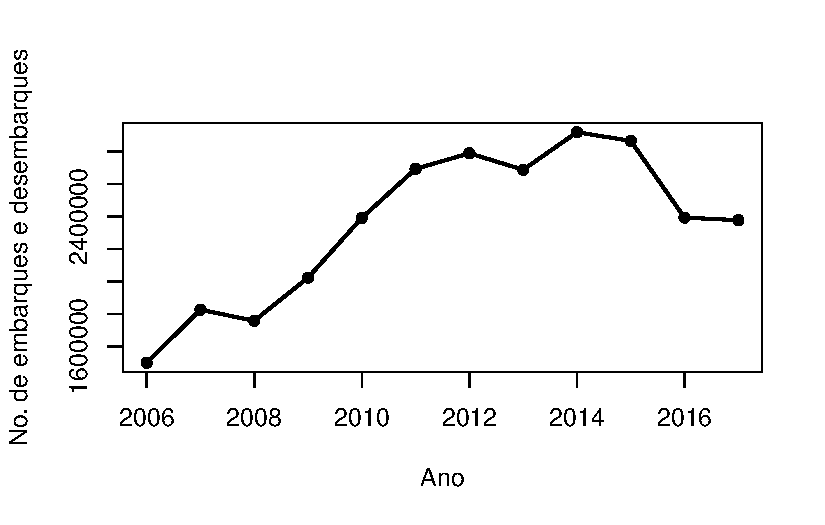
\includegraphics{intro_files/figure-pdf/unnamed-chunk-1-1.pdf}

Ainda considerando a série acima, seja \(x_t\) o número de embarques e
desembarques registrado no ano \(t\). A figura abaixo mostra o diagrama
de disperão entre \(x_t\) e \(x_{t-1}\), de onde é possível observar a
correlação positiva, estimada em 0,86.

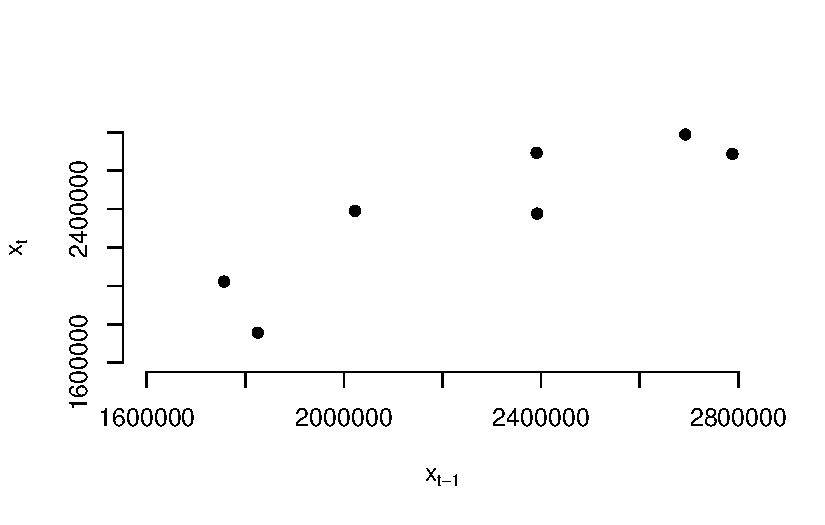
\includegraphics{intro_files/figure-pdf/unnamed-chunk-2-1.pdf}

De posse desses resultados, pode-se imaginar um primeiro modelo, no qual
a relação entre o presente e o passado imediato é ditado por uma
regressão linear simples, gerando a equação

\[\hat{x}_t = 7,589\times 10^5 +0,7109 x_{t-1}.\] Sabendo que
\(x_{2017}=2.376.505\), uma previsão para 2018 seria
\(\hat{x}_{2018}=2.448.357\). O valor observado em 2018 foi 2.572.159,
gerando um erro de previsão igual a \(x_{2018}-\hat{x}_{2018}=195.654\)
embarques e desembarques domésticos.

\hypertarget{exemplos-de-suxe9ries-temporais}{%
\section{Exemplos de séries
temporais}\label{exemplos-de-suxe9ries-temporais}}

\hypertarget{eletrocardiograma}{%
\subsection{Eletrocardiograma}\label{eletrocardiograma}}

\begin{Shaded}
\begin{Highlighting}[]
\FunctionTok{ts.plot}\NormalTok{(ECG)}
\end{Highlighting}
\end{Shaded}

\begin{figure}

\begin{minipage}[t]{\linewidth}

{\centering 

\raisebox{-\height}{

\includegraphics{intro_files/figure-pdf/unnamed-chunk-4-1.pdf}

}

\caption{1800 medidas da taxa cardíaca instantânea, em batidas por
minuto, de um indivíduo.}

}

\end{minipage}%

\end{figure}

\hypertarget{produto-interno-brupo-brasileiro}{%
\subsection{Produto Interno Brupo
Brasileiro}\label{produto-interno-brupo-brasileiro}}

\begin{Shaded}
\begin{Highlighting}[]
\FunctionTok{ts.plot}\NormalTok{(PIB)}
\end{Highlighting}
\end{Shaded}

\begin{figure}

\begin{minipage}[t]{\linewidth}

{\centering 

\raisebox{-\height}{

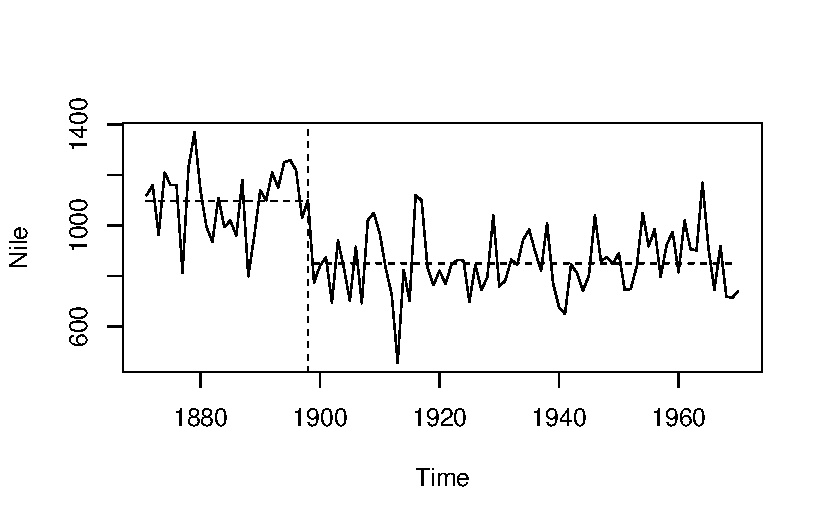
\includegraphics{intro_files/figure-pdf/unnamed-chunk-5-1.pdf}

}

\caption{PIB entre 1967 e 2014 corrigidos pelo valor do dólar em
4/2015.}

}

\end{minipage}%

\end{figure}

\hypertarget{mortes-por-doenuxe7as-pulmonares-no-reino-unido}{%
\subsection{Mortes por doenças pulmonares no Reino
Unido}\label{mortes-por-doenuxe7as-pulmonares-no-reino-unido}}

\begin{Shaded}
\begin{Highlighting}[]
\FunctionTok{ts.plot}\NormalTok{(ldeaths)}
\end{Highlighting}
\end{Shaded}

\begin{figure}

\begin{minipage}[t]{\linewidth}

{\centering 

\raisebox{-\height}{

\includegraphics{intro_files/figure-pdf/unnamed-chunk-6-1.pdf}

}

\caption{PIB entre 1967 e 2014 corrigidos pelo valor do dólar em
4/2015.}

}

\end{minipage}%

\end{figure}

\bookmarksetup{startatroot}

\hypertarget{criando-suxe9ries-no-r}{%
\chapter{\texorpdfstring{Criando séries no
\texttt{R}}{Criando séries no R}}\label{criando-suxe9ries-no-r}}

Esta seção tem por objetivo mostrar algumas funções em \texttt{R} para a
criação e análise exploratória de séries temporais.

\hypertarget{a-classe-ts}{%
\section{\texorpdfstring{A classe
\texttt{ts}}{A classe ts}}\label{a-classe-ts}}

Para todos os efeitos, uma série temporal é um vetor numérico. O vetor
abaixo armazena o número de nascidos vivos por mês na cidade de Manaus
em 2021, sendo \texttt{x{[}1{]}} o mês de janeiro e assim
sucessivamente.

\begin{Shaded}
\begin{Highlighting}[]
\NormalTok{x }\OtherTok{\textless{}{-}} \FunctionTok{c}\NormalTok{( }\DecValTok{3043}\NormalTok{, }\DecValTok{2902}\NormalTok{, }\DecValTok{3166}\NormalTok{, }\DecValTok{3014}\NormalTok{, }\DecValTok{3095}\NormalTok{, }\DecValTok{2955}\NormalTok{, }\DecValTok{3087}\NormalTok{, }\DecValTok{3141}\NormalTok{,}
\DecValTok{3129}\NormalTok{, }\DecValTok{3096}\NormalTok{, }\DecValTok{3191}\NormalTok{, }\DecValTok{3222}\NormalTok{)}
\end{Highlighting}
\end{Shaded}

Por sua vez, o gráfico da série temporal pode ser construído utilizando
a função \texttt{plot}, com o argumento
\texttt{type=\textquotesingle{}l\textquotesingle{}}.

\begin{Shaded}
\begin{Highlighting}[]
\FunctionTok{plot}\NormalTok{(x, }\AttributeTok{type =} \StringTok{\textquotesingle{}l\textquotesingle{}}\NormalTok{)}
\end{Highlighting}
\end{Shaded}

\begin{figure}[H]

{\centering \includegraphics{ts_window_date_files/figure-pdf/unnamed-chunk-2-1.pdf}

}

\end{figure}

Contudo, é útil construir a série temporal como um objeto da classe
\texttt{ts}. Tal função possui dois argumentos importantes:

\begin{itemize}
\item
  \texttt{frequency}: representa o número de observações por unidade de
  tempo. Por exemplo, se tempo está sendo contado em anos, mas o dados
  são mensais, então \texttt{frequency=12}; se os dados forem
  trimestrais, \texttt{frequency=4} e assim por diante.
\item
  \texttt{start}: representa o tempo da primeira observação. Pode ser
  representado por um único número ou por um vetor de comprimento dois.
  Esse último caso só é utilizado quando \texttt{frequency} é diferente
  de 1 e representa a ordem, em relação à frequência, da primeira
  observação. Por exemplo, com \texttt{frequency=12}, o vetor
  \texttt{start=c(1996,2)} implica que a primeira observação data de
  fevereiro de 1996.
\end{itemize}

No código abaixo, o vetor criado anteriormente é colocado com um objeto
\texttt{ts}

\begin{Shaded}
\begin{Highlighting}[]
\NormalTok{x }\OtherTok{\textless{}{-}} \FunctionTok{ts}\NormalTok{( x, }\AttributeTok{start =} \FunctionTok{c}\NormalTok{(}\DecValTok{2021}\NormalTok{,}\DecValTok{1}\NormalTok{), }\AttributeTok{frequency =} \DecValTok{12}\NormalTok{)}
\NormalTok{x}
\end{Highlighting}
\end{Shaded}

\begin{verbatim}
      Jan  Feb  Mar  Apr  May  Jun  Jul  Aug  Sep  Oct  Nov  Dec
2021 3043 2902 3166 3014 3095 2955 3087 3141 3129 3096 3191 3222
\end{verbatim}

\begin{Shaded}
\begin{Highlighting}[]
\FunctionTok{ts.plot}\NormalTok{(x)}
\end{Highlighting}
\end{Shaded}

\begin{figure}[H]

{\centering \includegraphics{ts_window_date_files/figure-pdf/unnamed-chunk-3-1.pdf}

}

\end{figure}

No gráfico acima, a parte decimal no eixo \(x\) representa a fração do
tempo entre de um ano (começando em 0 e acumulando 1/12 para cada mês
subsequente).

O gráfico pode ser customizado do mesmo modo que um \texttt{plot}.
Abaixo segue um exemplo.

\begin{Shaded}
\begin{Highlighting}[]
\FunctionTok{plot}\NormalTok{(x, }\AttributeTok{ylab =} \StringTok{\textquotesingle{}No. nascidos vivos mensal\textquotesingle{}}\NormalTok{, }\AttributeTok{lwd =} \DecValTok{2}\NormalTok{, }\AttributeTok{col =} \StringTok{\textquotesingle{}seagreen\textquotesingle{}}\NormalTok{)}
\end{Highlighting}
\end{Shaded}

\begin{figure}[H]

{\centering \includegraphics{ts_window_date_files/figure-pdf/unnamed-chunk-4-1.pdf}

}

\end{figure}

A função \texttt{start} retorna o início da série, \texttt{end} seu fim
e \texttt{frequency} o número de observações por unidade de tempo.
Observe o exemplo abaixo.

\begin{Shaded}
\begin{Highlighting}[]
\FunctionTok{start}\NormalTok{(x)}
\end{Highlighting}
\end{Shaded}

\begin{verbatim}
[1] 2021    1
\end{verbatim}

\begin{Shaded}
\begin{Highlighting}[]
\FunctionTok{end}\NormalTok{(x)}
\end{Highlighting}
\end{Shaded}

\begin{verbatim}
[1] 2021   12
\end{verbatim}

\begin{Shaded}
\begin{Highlighting}[]
\FunctionTok{frequency}\NormalTok{(x)}
\end{Highlighting}
\end{Shaded}

\begin{verbatim}
[1] 12
\end{verbatim}

A partir das informações acima, sabe-se a série \texttt{x} é mensal
(\texttt{frequency=12}), que sua primeira observação data de janeiro de
2021 e a última de dezembro de 2021.

\hypertarget{a-funuxe7uxe3o-window}{%
\section{\texorpdfstring{A função
\texttt{window}}{A função window}}\label{a-funuxe7uxe3o-window}}

A função \texttt{window} seleciona um subconjunto da série temporal.
Abaixo foram selecionados apenas os nascimentos entre Junho e Agosto e
este valores foram registrados no gráfico.

\begin{Shaded}
\begin{Highlighting}[]
\NormalTok{z }\OtherTok{\textless{}{-}} \FunctionTok{window}\NormalTok{(x, }\AttributeTok{start=}\FunctionTok{c}\NormalTok{(}\DecValTok{2021}\NormalTok{,}\DecValTok{6}\NormalTok{), }\AttributeTok{end =} \FunctionTok{c}\NormalTok{(}\DecValTok{2021}\NormalTok{,}\DecValTok{8}\NormalTok{))}

\FunctionTok{plot}\NormalTok{(x, }\AttributeTok{ylab =} \StringTok{\textquotesingle{}No. nascidos vivos mensal\textquotesingle{}}\NormalTok{, }\AttributeTok{lwd =} \DecValTok{2}\NormalTok{, }\AttributeTok{col =} \StringTok{\textquotesingle{}seagreen\textquotesingle{}}\NormalTok{)}
\FunctionTok{lines}\NormalTok{(z, }\AttributeTok{col =} \StringTok{\textquotesingle{}brown\textquotesingle{}}\NormalTok{, }\AttributeTok{lwd=} \DecValTok{2}\NormalTok{)}
\end{Highlighting}
\end{Shaded}

\begin{figure}[H]

{\centering \includegraphics{ts_window_date_files/figure-pdf/unnamed-chunk-6-1.pdf}

}

\end{figure}

\hypertarget{o-pacote-data.table}{%
\section{\texorpdfstring{O pacote
\texttt{data.table}}{O pacote data.table}}\label{o-pacote-data.table}}

Assim como números e textos possuem classes específicas, as datas no
ambiente \texttt{R} também possuem sua própria classe, denominada
\texttt{Date}.

\begin{Shaded}
\begin{Highlighting}[]
\CommentTok{\# 3 de agosto de 1998 (formato americano)}
\NormalTok{x }\OtherTok{\textless{}{-}} \StringTok{\textquotesingle{}1998/8/3\textquotesingle{}}
\FunctionTok{as.Date}\NormalTok{(x)}
\end{Highlighting}
\end{Shaded}

\begin{verbatim}
[1] "1998-08-03"
\end{verbatim}

Para que o \texttt{R} entenda uma data fora do padrão americano, é
necessário passar o formado para o argumento \texttt{format}. Seguem
alguns exemplos:

\begin{Shaded}
\begin{Highlighting}[]
\CommentTok{\# 3 de agosto de 1998 (formato nacional)}
\NormalTok{x }\OtherTok{\textless{}{-}} \StringTok{\textquotesingle{}3/8/1998\textquotesingle{}}
\FunctionTok{as.Date}\NormalTok{(x, }\AttributeTok{format =} \StringTok{\textquotesingle{}\%d/\%m/\%Y\textquotesingle{}}\NormalTok{)}
\end{Highlighting}
\end{Shaded}

\begin{verbatim}
[1] "1998-08-03"
\end{verbatim}

\begin{Shaded}
\begin{Highlighting}[]
\NormalTok{x }\OtherTok{\textless{}{-}} \StringTok{\textquotesingle{}3{-}8{-}1998\textquotesingle{}}
\FunctionTok{as.Date}\NormalTok{(x, }\AttributeTok{format =} \StringTok{\textquotesingle{}\%d{-}\%m{-}\%Y\textquotesingle{}}\NormalTok{)}
\end{Highlighting}
\end{Shaded}

\begin{verbatim}
[1] "1998-08-03"
\end{verbatim}

\begin{Shaded}
\begin{Highlighting}[]
\CommentTok{\# agosto de 1998}
\NormalTok{x }\OtherTok{\textless{}{-}} \StringTok{\textquotesingle{}8/1998\textquotesingle{}}
\FunctionTok{as.Date}\NormalTok{(x, }\AttributeTok{format =} \StringTok{\textquotesingle{}\%m/\%Y\textquotesingle{}}\NormalTok{)}
\end{Highlighting}
\end{Shaded}

\begin{verbatim}
[1] NA
\end{verbatim}

Ao se trabalhar com fontes originais, é comum ter como unidade amostral
um evento com sua data registrada. Em geral, nosso objetivo é determinar
a quantidade de eventos dentro de dias, semanas, meses ou anos. O pacote
\texttt{data.table} permite lidar com esse problema de modo rápido,
criando um objeto deste tipo utilizando a função \texttt{fread}.

Para ilustrar, será utilizada a base de dados de acidentes com
aeronaves, mantida pela Força Aérea Brasileira, que registra diariamente
o número de acidentes com aeronaves.

\begin{Shaded}
\begin{Highlighting}[]
\FunctionTok{library}\NormalTok{(data.table)}
\NormalTok{url }\OtherTok{\textless{}{-}} \StringTok{\textquotesingle{}https://drive.google.com/uc?authuser=0\&id=1iYrnwXgmLK07x8b330aD73scOVruZEuz\&export=download\textquotesingle{}}

\NormalTok{aereo }\OtherTok{\textless{}{-}}  \FunctionTok{fread}\NormalTok{(url, }\AttributeTok{encoding =} \StringTok{\textquotesingle{}Latin{-}1\textquotesingle{}}\NormalTok{)}
\NormalTok{aereo}\SpecialCharTok{$}\NormalTok{ocorrencia\_dia }\OtherTok{\textless{}{-}} \FunctionTok{as.Date}\NormalTok{(aereo}\SpecialCharTok{$}\NormalTok{ocorrencia\_dia, }\StringTok{\textquotesingle{}\%d/\%m/\%Y\textquotesingle{}}\NormalTok{)}
\end{Highlighting}
\end{Shaded}

Um objeto do tipo \texttt{data.table} permite uma série de consultas. Em
geral, pode-se fazer \texttt{aereo{[}a,b,c{]}}, onde \texttt{a} é uma
consulta/função nas linhas, \texttt{b} nas colunas e \texttt{c} é um
agrupador. Uma excelente introdução pode ser vista em
\href{https://cran.r-project.org/web/packages/data.table/vignettes/datatable-intro.html}{Introduction
to data.table}.

Abaixo, foi selecionada a coluna de interesse \texttt{ocorrencia\_dia}.

\begin{Shaded}
\begin{Highlighting}[]
\NormalTok{fab\_dia }\OtherTok{\textless{}{-}}\NormalTok{ aereo[,}\StringTok{\textquotesingle{}ocorrencia\_dia\textquotesingle{}}\NormalTok{,]}
\FunctionTok{head}\NormalTok{(fab\_dia)}
\end{Highlighting}
\end{Shaded}

\begin{verbatim}
   ocorrencia_dia
1:     2023-04-05
2:     2023-06-24
3:     2023-06-27
4:     2023-06-30
5:     2023-06-25
6:     2023-06-23
\end{verbatim}

Ao utilizar o operador \texttt{.N} em \texttt{{[},.N,c{]}}, é retornado
o número de linhas que possuem o agrupamento em \texttt{c}. Abaixo, as
datas do banco são agrupadas por ano.

\begin{Shaded}
\begin{Highlighting}[]
\NormalTok{fab\_ano }\OtherTok{\textless{}{-}}\NormalTok{ fab\_dia[, .N, by}\OtherTok{=}\NormalTok{.(}\FunctionTok{year}\NormalTok{(ocorrencia\_dia))]}
\NormalTok{fab\_ano }\OtherTok{\textless{}{-}}\NormalTok{fab\_ano[ }\FunctionTok{order}\NormalTok{(year) ]}
\FunctionTok{head}\NormalTok{(fab\_ano)}
\end{Highlighting}
\end{Shaded}

\begin{verbatim}
   year   N
1: 2013 654
2: 2014 569
3: 2015 471
4: 2016 403
5: 2017 432
6: 2018 444
\end{verbatim}

Os comandos a seguir criam dois objetos do tipo \texttt{ts}, sendo um
para o número anual de acidentes e outro para o mensal

\begin{Shaded}
\begin{Highlighting}[]
\NormalTok{fab\_ano }\OtherTok{\textless{}{-}} \FunctionTok{ts}\NormalTok{( fab\_ano, }\AttributeTok{start =} \DecValTok{2013}\NormalTok{)}
\FunctionTok{plot}\NormalTok{(fab\_ano[,}\DecValTok{2}\NormalTok{], }\AttributeTok{lwd =} \DecValTok{2}\NormalTok{, }\AttributeTok{ylab =} \StringTok{\textquotesingle{}No. acidentes/ano\textquotesingle{}}\NormalTok{, }\AttributeTok{xlab =} \StringTok{\textquotesingle{}Ano\textquotesingle{}}\NormalTok{)}
\end{Highlighting}
\end{Shaded}

\begin{figure}[H]

{\centering \includegraphics{ts_window_date_files/figure-pdf/unnamed-chunk-12-1.pdf}

}

\end{figure}

\begin{Shaded}
\begin{Highlighting}[]
\NormalTok{fab\_mes }\OtherTok{\textless{}{-}}\NormalTok{ fab\_dia[, .N, by}\OtherTok{=}\NormalTok{.(}\FunctionTok{year}\NormalTok{(ocorrencia\_dia), }\FunctionTok{month}\NormalTok{(ocorrencia\_dia))]}

\NormalTok{fab\_mes }\OtherTok{\textless{}{-}}\NormalTok{fab\_mes[ }\FunctionTok{order}\NormalTok{(year, month ) ]}
\NormalTok{fab\_mes }\OtherTok{\textless{}{-}} \FunctionTok{ts}\NormalTok{( fab\_mes[,}\DecValTok{3}\NormalTok{], }\AttributeTok{start =} \FunctionTok{c}\NormalTok{(}\DecValTok{2013}\NormalTok{, }\DecValTok{1}\NormalTok{), }\AttributeTok{frequency =} \DecValTok{12}\NormalTok{)}
\FunctionTok{plot}\NormalTok{(fab\_mes, }\AttributeTok{lwd =} \DecValTok{2}\NormalTok{, }\AttributeTok{ylab =} \StringTok{\textquotesingle{}No. acidentes/mês\textquotesingle{}}\NormalTok{, }\AttributeTok{xlab =} \StringTok{\textquotesingle{}Ano\textquotesingle{}}\NormalTok{)}
\end{Highlighting}
\end{Shaded}

\begin{figure}[H]

{\centering \includegraphics{ts_window_date_files/figure-pdf/unnamed-chunk-12-2.pdf}

}

\end{figure}

\hypertarget{exercuxedcio}{%
\section{Exercício}\label{exercuxedcio}}

Exercício 1

A série abaixo contém a data dos óbitos maternos no Brasil a partir de
2010.

\begin{Shaded}
\begin{Highlighting}[]
\NormalTok{url }\OtherTok{\textless{}{-}} \StringTok{\textquotesingle{}https://drive.google.com/uc?authuser=0\&id=1tYFFT9L2iopKmBDUI3P8qNIRaOnMYj7d\&export=download\textquotesingle{}}
\end{Highlighting}
\end{Shaded}

Crie uma série temporal com o número de óbitos mensal e faça um gráfico.
Crie uma janela para colocar no gráfico o período da pandemia de
COVID-19.

\bookmarksetup{startatroot}

\hypertarget{suxe9ries-estacionuxe1rias}{%
\chapter{Séries Estacionárias}\label{suxe9ries-estacionuxe1rias}}

Uma coleção do tipo \(\{x(t),t\in\mathcal{T}\}\),
\(\mathcal{T}\subseteq \mathbb{R}\), onde \(x(t)\) é uma variável
aleatória para cada \(t\) fixado, é denominada processo estocástico.

Um processo estocástico é dito ser fortemente estacionário se sua
distribuição é invariante ao índice. Portanto, para qualquer
\(t_1,\ldots,t_k\), a distribuição de \(x(t_1),\ldots,x(t_k)\) é a mesma
de \(x(t_1+h),\ldots,x(t_k+h)\).

\begin{example}[]\protect\hypertarget{exm-serie_estacionaria_1}{}\label{exm-serie_estacionaria_1}

Se \(x(t)\sim \hbox{Normal}(0,1)\) e \(x(t)\) é independente de \(x(s)\)
para todo \(t\neq s\), então, para qualquer \(t_1,\ldots,t_k\),

\[\begin{align}P(x(t_1)<x_1,\ldots,x(t_k)<x_k)&=\prod_{i=1}^k P(x(t_i)<x_i)=\prod_{i=1}^k P(x(t_i+h)<x_i)\\&=P(x(t_1+h)<x_1,\ldots,x(t_k+h)<x_k)\end{align}\]
logo, \(\{x(t),t\in \mathbb{R}\}\) é um processo fortemente
estacionário. \(\blacksquare\)

\end{example}

\begin{theorem}[]\protect\hypertarget{thm-exm_estacionaria2}{}\label{thm-exm_estacionaria2}

Seja \(\{x(t),t\in\mathbb{N}\}\) um processo estocástico com
\[x(t)= x_{(t-1)}+\varepsilon_t,\;\;\varepsilon_t\sim\hbox{Normal}(0,1),\]
para \(t=1,2,\ldots\) com a condição de que
\(x_0\sim\hbox{Normal}(0,1)\) e que
\(Cov(\varepsilon_t,\varepsilon_s)=0\;\;\forall s\neq t\). Então,
\[x_t=x_{t-1}+\varepsilon_{t}=\cdots=x_0+\sum_{j=1}^t\varepsilon_t\sim\hbox{Normal}(0,t+1).\]
Como \(x_t\sim\hbox{Normal}(0,t+1)\) e, para qualquer \(h>0\),
\(x_{t+h}\sim\hbox{Normal}(0,t+h+1)\), temos que este processo não é
fortemente estacionário. \(\blacksquare\)

\end{theorem}

\begin{definition}[]\protect\hypertarget{def-fracamente}{}\label{def-fracamente}

Um processo estocástico \(\{y_t\}\) é dito ser fracamente estacionário
(ou de segunda ordem) se \[\begin{align*}
    E(y_t)&=\mu,\\
    Var(y_t)&=\nu,\\ 
    Cov(y_t,y_s)&=E(y_ty_s)-E(y_t)E(y_s)=\gamma(t-s)
    \end{align*}\] onde \(\mu\) e \(\nu\) são constantes independentes
de \(t\) e \(\gamma(t-s)\) depende de \(t\) e \(s\) somente através da
diferença \(|t-s|\). \(\blacksquare\)

\end{definition}

\begin{example}[]\protect\hypertarget{exm-fracamente1}{}\label{exm-fracamente1}

Considere o processo estocástico \(\{x(t),t\in\mathbb{N}\}\), onde
\[x(t) = \varepsilon(t) +\frac{1}{2}\varepsilon(t-1)
\] onde \(\varepsilon(t)\sim\hbox{Normal}(0,\nu)\) para \(t=1,\ldots\),
\(\varepsilon(t)\) é independente de \(\varepsilon(s)\) para todo
\(s\neq t\) e \(\varepsilon(0)=0\). Então: \[\begin{align}
E(x(t))&=E(\varepsilon(t))+\frac{1}{2}E(\varepsilon(t-1))=0\\
Var(x(t))&=Var(\varepsilon(t))+\frac{1}{4}Var(\varepsilon(t-1))=\frac{5}{4}\nu
\end{align}
\] e \[\begin{align}
          Cov(x(t),x(t+h))&=Cov\left(\varepsilon(t)+\frac{1}{2}\varepsilon(t-1),\varepsilon(t+h)+\frac{1}{2}\varepsilon(t+h-1)\right)\\
          &=Cov\left(\varepsilon(t),\varepsilon(t+h)\right)+\frac{1}{2}Cov\left(\varepsilon(t),\varepsilon(t+h-1)\right)\\
          &+\frac{1}{2}Cov\left(\varepsilon(t-1),\varepsilon(t+h)\right)+\frac{1}{4}Cov\left(\varepsilon(t-1),\varepsilon(t+h-1)\right)\\
          &=\left\{ \begin{array}{ll}
          \frac{4}{5}\nu,&\; h = 0 \\         
          \frac{1}{2}\nu,&\; |h|=1,\\
          0,&\;\hbox{caso contrário.}
          \end{array} \right.
    \end{align}\] Portanto, o processo é fracamente estacionáriao.
\(\blacksquare\)

\end{example}

Quando \(\mathcal{T}=\{t\in D\subseteq \mathbb{Z}\}\), utiliza-se a
notação \(x(t)=x_t\). Além disso, se \(t\) pode ser interpretado como
tempo, \(x_t\) é uma série temporal. Uma série temporal é dita ser
estacionária se ela é fracamente estacionária e o mesmo princípio se
aplica nessas notas de aula.

\hypertarget{processo-estacionuxe1rio-erguxf3dico}{%
\section{Processo estacionário
ergódico}\label{processo-estacionuxe1rio-erguxf3dico}}

Seja \(x_1,x_2,\ldots,x_n\) uma série temporal estacionária. Então, a
média \(\mu\) pode ser estimada por \(\bar{x}_n\), uma vez que
\(E(\bar{x})=\mu\). A variância essa estatística é

\[\begin{align}Var(\bar{x})&=Cov(\bar{x}_n,\bar{x}_n)=Cov\left(\sum_{i=1}^n \frac{x_i}{n},\sum_{j=1}^n\frac{x_j}{n}\right)=\frac{1}{n^2}\sum_{i=1}^n\sum_{j=1}^nCov(x_i,x_j)\\
&=\frac{1}{n^2}\left[\sum_{i=1}^nCov(x_i,x_i)+2\sum_{i=1}^n\sum_{j\neq i}Cov(x_i,x_j)\right]\\
&=\frac{1}{n^2}\left[n\nu+2\sum_{h=1}^{n-1}(n-h)\gamma(h)\right]=\frac{\nu}{n}+\frac{2}{n}\sum_{h=1}^{n-1}\left(1-\frac{h}{n}\right)\gamma(h)
\end{align}\]

Note que, diferente do caso independente e identicamente distribuído,
\(\bar{x}\) não é necessariamente um estimador adequado, conforme pode
ser constatado no exemplo abaixo.

\begin{example}[]\protect\hypertarget{exm-estationario_nao_ergodico}{}\label{exm-estationario_nao_ergodico}

Seja \(x_t\) um processo onde \(x_0\sim\hbox{Normal}(0,\nu)\) e
\(x_t=x_0\) para todo \(t>0\). Como

\[\begin{align}
E(x_t)&=E(E(x_t|x_0))=E(x_0)=0\\
Var(x_t)&=E(Var(x_t|x_0))+Var(E(x_t|x_0))=E(0)+Var(x_0)=\nu\\
Cov(x_t,x_{t-h})&=E( Cov(x_t,x_{t-h}|x_0))+Cov( E(x_t|x_0),E(x_{t-h}|x_0))\\
&=E(0)+Cov(x_0,x_0)=Var(x_0)=\nu
\end{align}\] e, portanto, o processo é fracamente estacionário.
Contudo,
\[Var(\bar{x})=\frac{\nu}{n}+\frac{2}{n}\sum_{h=1}^{n-1}\left(1-\frac{h}{n}\right)\nu=\nu,\]
portanto, o erro padrão não decai com o aumento do tamanho da amostra.

\(\blacksquare\)

\end{example}

A partir do exemplo acima, fica claro que \(\bar{x}\) nem sempre será um
estimador adequado para uma série estacionária.

\begin{definition}[]\protect\hypertarget{def-ergodica}{}\label{def-ergodica}

Uma série temporal estacionária é dita ser ergódica para a média se
\[\sum_{i=1}^n\frac{x_1}{n}\stackrel{p}{\rightarrow} \mu,\] quando
\(n\rightarrow\infty\).

\end{definition}

A partir deste momento será considerado que toda série temporal
estacionária é ergódica e, portanto \(\bar{x}\) é um estimador para
\(\mu\).

\begin{example}[]\protect\hypertarget{exm-estationario_nao_ergodico_conclusao}{}\label{exm-estationario_nao_ergodico_conclusao}

Considere novamente o processo no
(\textbf{estationario\_nao\_ergodico?}). Como \(\bar{x}_n=x_0\), tem-se
que, para \(\varepsilon>0\) arbitrário,
\(\bar{x}\sim\hbox{Normal}(0,\nu)\) e
\[P(|\bar{x}_n-0|>\varepsilon)=2P(x_0>\varepsilon)=2\int_{-\infty}^\varepsilon \frac{1}{\sqrt{2\pi\nu}}e^{-\frac{y^2}{2\nu}}d\nu>\frac{1}{2}\]
logo, \(\bar{x}\) não converge em probabilidade para \(0\) e, portanto,
o processo não é ergódico na média. \(\blacksquare\)

\end{example}

\hypertarget{ruuxeddo-branco}{%
\section{Ruído branco}\label{ruuxeddo-branco}}

\begin{definition}[]\protect\hypertarget{def-ruido_branco}{}\label{def-ruido_branco}

A série estacionária \(x_t\) é dita ser um ruído branco se \(E(x_t)=0\),
\(Var(x_t)=\nu\) e \[\begin{equation}
        Cov(x_t,x_s)=0,
        \end{equation}\] para todo \(t\neq s\). \(\blacksquare\)

\end{definition}

É imediato que o ruído branco é uma série temporal estacionária. Além
disso, pela Desigualdade de Chebyshev, para qualquer \(\varepsilon>0\),

\[P\left(|\bar{x}_n|\geq\varepsilon\right)\leq \frac{E(\bar{x}_n^2)}{\varepsilon^2}=\frac{Var(\bar{x}_n)}{\varepsilon^2}=\frac{\nu}{n\varepsilon^2}\]
logo \(\lim_{n}P(|\bar{x}_n|\leq \varepsilon)=0\) e
\(\bar{x}_n\stackrel{p}{\rightarrow}0\). Portanto, o ruído branco é
ergódico.

Considere agora a série temporal \(y_t=\mu+x_t\), onde \(x_t\) é um
ruído branco. Então
\[\bar{y}_n=\mu+\bar{x}_n\stackrel{p}{\rightarrow}\mu\] e \(\bar{y}_n\)
é um estimador para \(\mu\).

Em certos momentos, será considerado que \(x_t\) e \(x_s\), para todo
\(t\neq s\) são independentes (essa é uma condição mais forte, pois
implica em \(Cov(x_t,x_s)=0\)). Esse processo é denominado ruído branco
independente.

Por último, também será considerado a possibilidade de que
\(x_t\sim\hbox{Normal}(0,\nu)\), com \(x_t\) e \(x_s\) indepentens para
todo \(t\neq s\). Esse processo será denominado é denominado ruído
branco gaussiano.

\bookmarksetup{startatroot}

\hypertarget{revisuxe3o-sobre-o-modelo-linear}{%
\chapter{Revisão sobre o modelo
linear}\label{revisuxe3o-sobre-o-modelo-linear}}

\hypertarget{definiuxe7uxe3o}{%
\section{Definição}\label{definiuxe7uxe3o}}

Para \(i=1,\ldots,n\), considere o modelo linear abaixo:
\[y_i= \beta_0+\sum_{j=1}^{p-1}x_{i,j}+\varepsilon_i=\underbrace{ \left(1\;\;x_{i,1}\;\;\cdots\;\;x_{i,p-1}\right)}_\text{$\boldsymbol{f}'_i$}\underbrace{\left(\begin{array}{c}\beta_0 \\ \beta_1 \\ \vdots \\ \beta_{p-1} 
        \end{array}\right)}_\text{$\boldsymbol{\beta}$}+\varepsilon_i=\boldsymbol{f}'_i\boldsymbol{\beta}+\varepsilon_i,\]
onde \(x_i\) é fixado e \(\varepsilon\) é um ruído branco gaussiano.
Pela independência entre \(y_i\) e \(y_j\), pode-se fazer a seguinte
representação estocástica de \(\boldsymbol{y}\): \[\begin{equation}
        \boldsymbol{y}=\boldsymbol{F}'\boldsymbol{\beta} + \boldsymbol{\varepsilon},
        \end{equation}\] onde
\(\boldsymbol{\varepsilon}\sim\hbox{Normal}(\boldsymbol{0},\nu\textbf{I}_n)\)
e \(\boldsymbol{F}\) é uma matriz \(p\times n\) conhecida com
\(i\)-ésima coluna dada por \(\boldsymbol{f}_i\):

\[\boldsymbol{F}=\left(\boldsymbol{f}_1,\ldots,\boldsymbol{F}\right).\]

A função de verossimilhança é dada por \[\begin{align*}
    L(\boldsymbol{\beta},\nu)&\propto \left(\frac{1}{v}\right)^{\frac{T}{2}}\exp\left\{-\frac{1}{2\nu}(\boldsymbol{y}-\boldsymbol{F}'\boldsymbol{\beta})'(\boldsymbol{y}-\boldsymbol{F}'\boldsymbol{\beta}) \right\}\\
    &\propto \left(\frac{1}{v}\right)^{\frac{T}{2}}\exp\left\{-\frac{1}{2\nu}\left[(\boldsymbol{\beta}-\hat{\boldsymbol{\beta}})'\boldsymbol{F}\boldsymbol{F}'(\boldsymbol{\beta}-\hat{\boldsymbol{\beta}}) + R\right]\right\}\\
    \end{align*}\] onde \[\begin{align}
    \hat{\boldsymbol{\beta}}&=\left(\boldsymbol{F}\boldsymbol{F}'\right)^{-1}\boldsymbol{F}\boldsymbol{y},\\
    R &= \left( \boldsymbol{y}-\boldsymbol{F}' \hat{\boldsymbol{\beta}}\right)' \left( \boldsymbol{y}-\boldsymbol{F}' \hat{\boldsymbol{\beta}}\right)   
    \end{align}\]

É sabido que:

\begin{itemize}
\item
  \(\hat{\boldsymbol{\beta}}\) é o estimador de máxima verossimilhança
  de \(\boldsymbol{\beta}\)
\item
  \(R\) é conhecido como \emph{soma de quadrados de resíduos}
\item
  \(\hat{\nu}=R/(n-p)\) é um estimador não viciado para \(\nu\).
\end{itemize}

Além disso, tem-se que

\[\begin{align*}
     \hat{\boldsymbol{\beta}}&\sim\hbox{Normal}_p(\boldsymbol{\beta},(\boldsymbol{F}\boldsymbol{F}'_n)^{-1}\nu)\\
     \frac{R}{\nu}&\sim\chi^2_{n-p}\\
     \sqrt{n-p}\frac{\hat{\boldsymbol{\beta}}-\boldsymbol{\beta}}{\sqrt{R}}&\sim t_{n-p}(\boldsymbol{0}_p, (\boldsymbol{F}'\boldsymbol{F})^{-1})
     \end{align*}\]

\hypertarget{resuxedduos-e-valores-ajustados}{%
\section{Resíduos e valores
ajustados}\label{resuxedduos-e-valores-ajustados}}

O valor ajustado da \(i\)-ésima observação é dado por \[\begin{equation}
        \hat{y}_i=\boldsymbol{f}_i' \hat{\boldsymbol{\beta}}
        \end{equation}\] e, concluímos que
\[\hat{\boldsymbol{y}}\sim \hbox{Normal}( \boldsymbol{F}'\boldsymbol{\beta}, \boldsymbol{F}'(\boldsymbol{F}\boldsymbol{F}')^{-1}\boldsymbol{F}\nu )\]

O respectivo resíduo é dado por \[e_i=y_i - \hat{y}_i,\] e, como o vetor
de resíduos é dado por
\[\boldsymbol{e}=\boldsymbol{y}-\hat{\boldsymbol{y}},\] tem-se que
\[\boldsymbol{e}\sim \hbox{Normal}(\boldsymbol{0}_n,\nu(\boldsymbol{I}_n-\boldsymbol{F}'(\boldsymbol{F}\boldsymbol{F}')^{-1}\boldsymbol{F}))\]
Denotando
\(\boldsymbol{H}=\boldsymbol{F}'(\boldsymbol{F}\boldsymbol{F}')^{-1}\boldsymbol{F})\),
de \(h_i\) como sendo o \(i\)-ésimo elemento na diagonal de
\(\boldsymbol{H}\), defini-se o resíduo studentizado por

\[\tilde{e}_i=\frac{e_i}{\sqrt{\hat{\nu}(1-h_i)}}\] Acontece que, se a
suposição de ruído btanco gaussiano for verdadeira, \(\tilde{e}_i\)
tende a se comportar como um ruído branco.

\hypertarget{seleuxe7uxe3o-de-modelos}{%
\section{Seleção de modelos}\label{seleuxe7uxe3o-de-modelos}}

Modelos lineares podem ser comparados através do critério de informação
de Akaike (AIC):

\[-2\log L(\hat{\boldsymbol{\beta}},\hat{\nu}) - 2(p+1).\]

Considera-se como mais parcimonioso o modelo com menor valor do AIC.

\hypertarget{robustez-do-modelo-linear}{%
\section{Robustez do modelo linear}\label{robustez-do-modelo-linear}}

Embora tenhamos utilizado o ruído branco gaussiano, estes resultados
ainda podem ser aplicados quando \(\varepsilon_n\) é um ruído branco
qualquer.

De fato, pode-se mostrar que os estimadores são os mesmos obtidos pelo
método dos mínimos quadrados. Neste caso, as distribuições dos
estimadores podem ser utilizadas como aproximações.

\bookmarksetup{startatroot}

\hypertarget{tenduxeancia}{%
\chapter{Tendência}\label{tenduxeancia}}

\hypertarget{o-que-uxe9-tenduxeancia}{%
\section{O que é tendência?}\label{o-que-uxe9-tenduxeancia}}

Diz-se que uma série temporal observada possui tendência quando ela
exibe um padrão de crescimento ou decrescimento em médio/longo prazo.

A Figure~\ref{fig-fabMes} mostra a série do número mensal de acidentes
com aeronaves, construída através dos dados diários mantidos pela Força
Aérea Brasileira. Note uma tendência de decrescimento na série até
meados de 2016, substituída então por uma tendência de crescimento.

\begin{Shaded}
\begin{Highlighting}[]
\NormalTok{url }\OtherTok{\textless{}{-}} \StringTok{\textquotesingle{}https://www.dropbox.com/scl/fi/kq4jwbovu94u857238sus/N{-}mensal{-}de{-}acidentes{-}com{-}aeronaves{-}2013jan.csv?rlkey=n5pa45e7ht33houmiawdkjb09\&dl=1\textquotesingle{}}

\NormalTok{x }\OtherTok{\textless{}{-}} \FunctionTok{read.csv}\NormalTok{(url, }\AttributeTok{h =}\NormalTok{ T)}
\NormalTok{acidentesFAB }\OtherTok{\textless{}{-}} \FunctionTok{ts}\NormalTok{( x, }\AttributeTok{start =} \FunctionTok{c}\NormalTok{(}\DecValTok{2013}\NormalTok{,}\DecValTok{1}\NormalTok{), }\AttributeTok{frequency=}\DecValTok{12}\NormalTok{)}
\FunctionTok{ts.plot}\NormalTok{(acidentesFAB, }\AttributeTok{lwd =} \DecValTok{2}\NormalTok{, }\AttributeTok{xlab =} \StringTok{\textquotesingle{}Ano\textquotesingle{}}\NormalTok{, }\AttributeTok{ylab =} \StringTok{\textquotesingle{}No. acidentes\textquotesingle{}}\NormalTok{)}
\end{Highlighting}
\end{Shaded}

\begin{figure}

\begin{minipage}[t]{\linewidth}

{\centering 

\raisebox{-\height}{

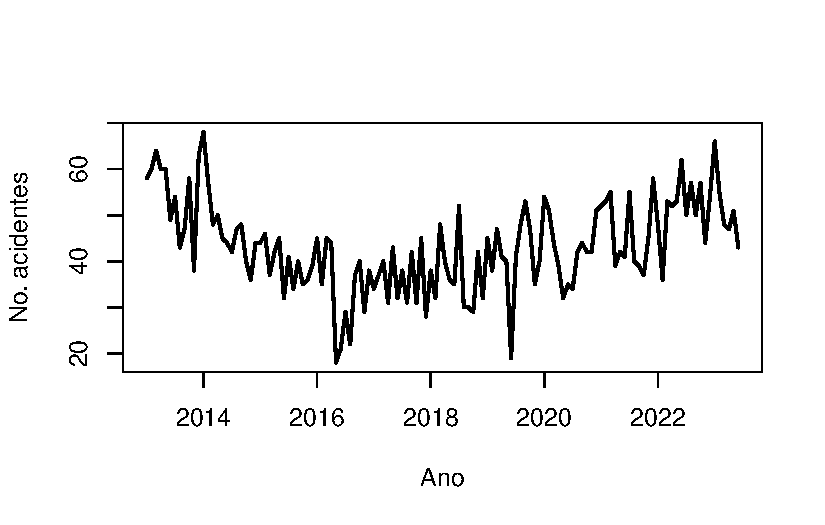
\includegraphics{tendencia_files/figure-pdf/fig-fabMes-1.pdf}

}

\caption{\label{fig-fabMes}Número mensal de acidentes envolvendo
aeronaves. Fonte: FAB}

}

\end{minipage}%

\end{figure}

\hypertarget{tenduxeancia-aletuxf3ria-e-tenduxeancia-determinuxedstica}{%
\section{Tendência aletória e tendência
determinística}\label{tenduxeancia-aletuxf3ria-e-tenduxeancia-determinuxedstica}}

A tendência pode ser duas naturezas: determinística ou aleatória.

A tendência aleatória é construída ao acaso. Considere, por exemplo, o
passeio aleatório definido por \(x_0=0\) e
\(x_t = x_{t-1}+\varepsilon_t\), onde \(\varepsilon_t\) é um ruído
branco gaussiano com \(\nu=1\). Já foi mostrado que \(E(x_t)=0\) e
\(Var(x_t)=t\). A figura abaixo apresenta uma série simulada desse
processo.

\begin{Shaded}
\begin{Highlighting}[]
\FunctionTok{set.seed}\NormalTok{(}\DecValTok{1}\NormalTok{)}
\NormalTok{x }\OtherTok{=} \DecValTok{0}
\ControlFlowTok{for}\NormalTok{( t }\ControlFlowTok{in} \DecValTok{2}\SpecialCharTok{:}\DecValTok{100}\NormalTok{) x[t] }\OtherTok{=}\NormalTok{ x[t }\SpecialCharTok{{-}} \DecValTok{1}\NormalTok{] }\SpecialCharTok{+} \FunctionTok{rnorm}\NormalTok{(}\DecValTok{1}\NormalTok{,}\DecValTok{0}\NormalTok{,}\DecValTok{1}\NormalTok{)}
\FunctionTok{ts.plot}\NormalTok{(x, }\AttributeTok{lwd =} \DecValTok{2}\NormalTok{)}
\end{Highlighting}
\end{Shaded}

\begin{figure}[H]

{\centering 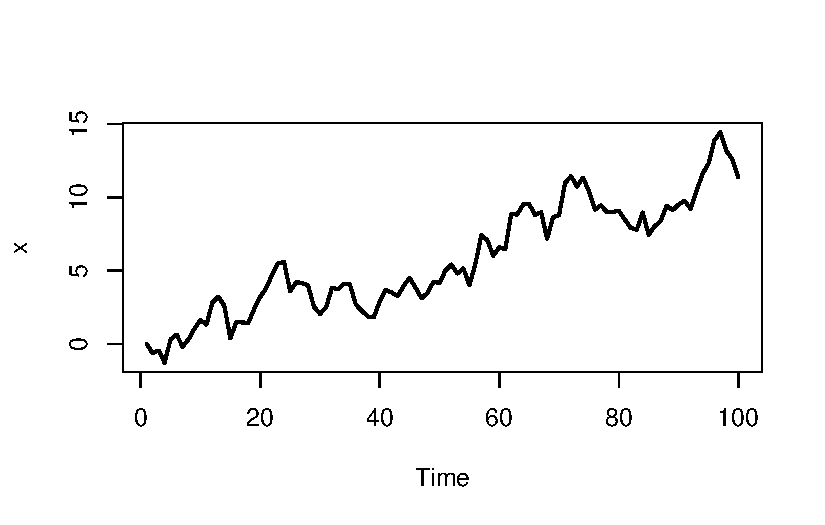
\includegraphics{tendencia_files/figure-pdf/unnamed-chunk-2-1.pdf}

}

\end{figure}

Observe que a série exibe um tendência, mas não há qualquer explicação
para a sua exsitência, uma vez que este comportamento é fruto do acaso.
Ainda, teremos que \(E(x_t)=0\), o que torna o padrão observado
irrelevante.

Na tendência determinística, há uma função T(.) que determina seu
comportamento. Nesse caso, é assumido que

\[y_t = T(t) + \varepsilon_t,\] onde \(\varepsilon_t\) é uma série
estacionária com média \(0\) e variância \(\nu\). Deste modo,
\(E(y_t)=T(t)\), o que implica que \(T(.)\) representa o comportamento
médio da série. O problema de estimar \(T(.)\) é denominado suavização.

Na prática, é impossível determinar se uma tendência é aleatória ou
determinística, cabendo ao estastístico procurar se há motivos para
acreditar que está analisando o segundo tipo. A partir deste momento,
toda tendência será considerada determinística.

\hypertarget{o-modelo-de-tenduxeancia-polinomial}{%
\section{O modelo de tendência
polinomial}\label{o-modelo-de-tenduxeancia-polinomial}}

Considere que a série temporal foi observada até o tempo \(s\). Então, a
tendência é definida como uma função \(T:(0,t]\rightarrow \mathbb{R}\).
O Teorema de Weierstrass afirma que, se \(T\) é contínua, então para
qualquer \(\delta>0\), existe um polinômio \(u(.)\) tal que
\[|T(t)-u(t)|<\delta.\] Isto quer dizer que \(T(.)\) sempre pode ser
aproximada por um polinômio. Assim, para determinada ordem \(p\), é
correto afirmar que\\
\[\begin{equation}
        y_t = \beta_0 + \sum_{j=1}^p \beta_j t^j + \varepsilon_t
        \end{equation}\] onde \(\varepsilon_t\) é uma série
estacionária, é um modelo razoável para uma série temporal com
tendência. Assumindo que \(\varepsilon_t\) é um ruído branco gaussiano,
tem-se o modelo de tendência polinomial de grau \(p\).

Fazendo \(\boldsymbol{f}_t'=(1,t,\ldots,t^p)\) , o modelo de tendência
polinomial é reescrito como
\[\boldsymbol{y}=\boldsymbol{F}'\boldsymbol{\beta}+\boldsymbol{\varepsilon}\]
e inferências sobre \(\boldsymbol{\beta}\) e \(\nu\) são feitas
utilizando o modelo linear tradicional.

\begin{example}[]\protect\hypertarget{exm-nascidos}{}\label{exm-nascidos}

Considere o número anual de nascidos vivos no estado do Amazonas entre
os anos 2000 e 20013:

\begin{Shaded}
\begin{Highlighting}[]
\NormalTok{x }\OtherTok{\textless{}{-}} \FunctionTok{c}\NormalTok{( }\DecValTok{67646}\NormalTok{ , }\DecValTok{70252}\NormalTok{ , }\DecValTok{70671}\NormalTok{ , }\DecValTok{70751}\NormalTok{ , }\DecValTok{71345}\NormalTok{ ,}
        \DecValTok{73488}\NormalTok{ , }\DecValTok{75584}\NormalTok{ , }\DecValTok{73469}\NormalTok{ , }\DecValTok{75030}\NormalTok{ , }\DecValTok{75729}\NormalTok{ , }
        \DecValTok{74188}\NormalTok{ , }\DecValTok{76202}\NormalTok{ , }\DecValTok{77434}\NormalTok{ , }\DecValTok{79041}\NormalTok{)}

\NormalTok{nascidos }\OtherTok{\textless{}{-}} \FunctionTok{ts}\NormalTok{(x, }\AttributeTok{start =}\DecValTok{2000}\NormalTok{)}
\end{Highlighting}
\end{Shaded}

\begin{Shaded}
\begin{Highlighting}[]
\FunctionTok{ts.plot}\NormalTok{(nascidos, }\AttributeTok{lwd =} \DecValTok{2}\NormalTok{, }\AttributeTok{ylab =} \StringTok{\textquotesingle{}No. nascidos vivos\textquotesingle{}}\NormalTok{)}
\NormalTok{stats}\SpecialCharTok{::}\FunctionTok{acf}\NormalTok{(nascidos)}
\end{Highlighting}
\end{Shaded}

\begin{figure}

\begin{minipage}[t]{0.50\linewidth}

{\centering 

\raisebox{-\height}{

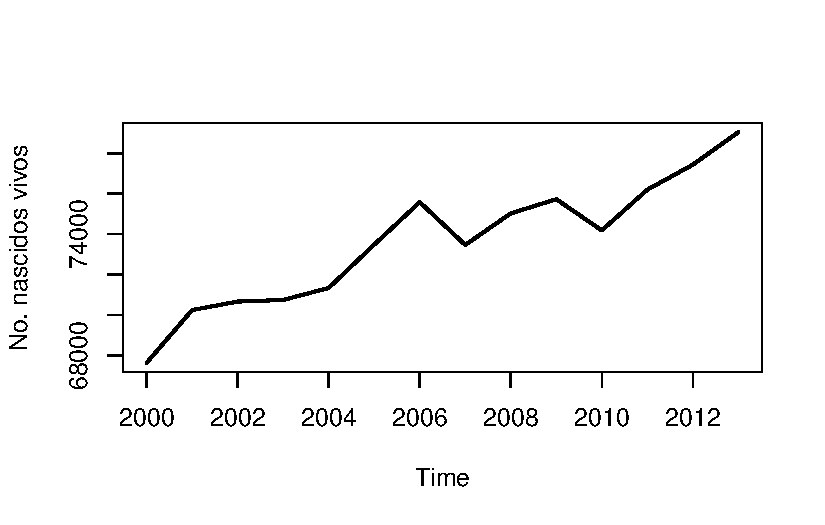
\includegraphics{tendencia_files/figure-pdf/fig-nascidosAM-1.pdf}

}

\caption{\label{fig-nascidosAM-1}Número de nascimentos anual no estado
do Amazonas (Fonte: SINASC/SUS)}

}

\end{minipage}%
%
\begin{minipage}[t]{0.50\linewidth}

{\centering 

\raisebox{-\height}{

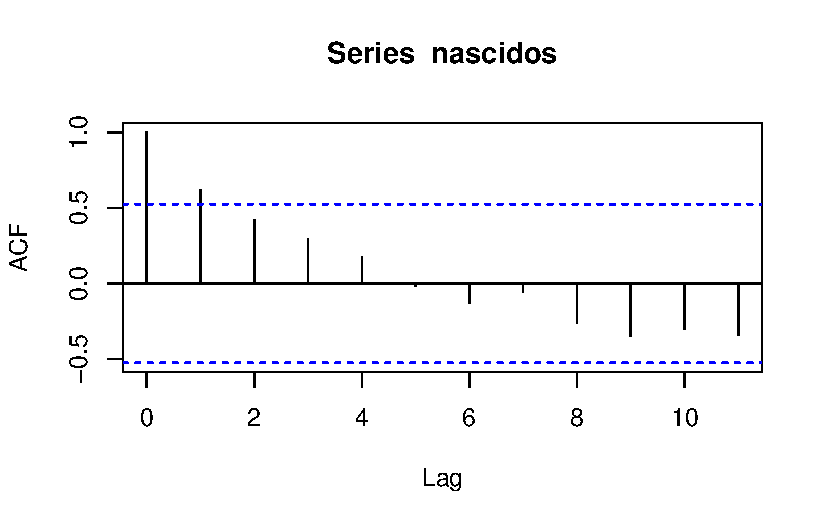
\includegraphics{tendencia_files/figure-pdf/fig-nascidosAM-2.pdf}

}

\caption{\label{fig-nascidosAM-2}Correlograma da série (Fonte:
SINASC/SUS).}

}

\end{minipage}%

\end{figure}

Vamos ajustar um modelo de tendência polinomial de ordem 1, ou seja

\[y_t=\beta_0+\beta_1 t + \varepsilon_t\] onde \(t=1,\ldots,14\)
representa os tempos \(2000,\ldots,2013\).

\begin{Shaded}
\begin{Highlighting}[]
\NormalTok{tempo }\OtherTok{\textless{}{-}} \DecValTok{1}\SpecialCharTok{:}\DecValTok{14}
\NormalTok{mod }\OtherTok{\textless{}{-}} \FunctionTok{lm}\NormalTok{( nascidos }\SpecialCharTok{\textasciitilde{}} \FunctionTok{poly}\NormalTok{(tempo, }\DecValTok{1}\NormalTok{, }\AttributeTok{raw =} \ConstantTok{TRUE}\NormalTok{))}
\end{Highlighting}
\end{Shaded}

As estimativas de máxima verossimilhança para \(\beta_0\) e \(\beta_1\)
são:

\begin{Shaded}
\begin{Highlighting}[]
\NormalTok{mod}\SpecialCharTok{$}\NormalTok{coefficients}
\end{Highlighting}
\end{Shaded}

\begin{verbatim}
               (Intercept) poly(tempo, 1, raw = TRUE) 
                 68266.879                    715.178 
\end{verbatim}

ou seja, \[\hat{T}(t)=\hat{\beta}+\hat{\beta}_1 t = 68.267+715 t\] Os
resíduos do modelo linear \texttt{mod} podem ser obtidos via função
\texttt{residuals}. Abaixo, verificamos que a série dos resíduos oscila
em torno de zero e que nenhuma autocorrelação parece ser relevante, o
que dão indícios de que os erros são um ruído branco.

\begin{Shaded}
\begin{Highlighting}[]
\NormalTok{res }\OtherTok{\textless{}{-}} \FunctionTok{residuals}\NormalTok{(mod)}
\FunctionTok{ts.plot}\NormalTok{( res, }\AttributeTok{main =} \StringTok{\textquotesingle{}\textquotesingle{}}\NormalTok{)}
\FunctionTok{acf}\NormalTok{(res, }\AttributeTok{main =} \StringTok{\textquotesingle{}\textquotesingle{}}\NormalTok{)}
\end{Highlighting}
\end{Shaded}

\begin{figure}

\begin{minipage}[t]{0.50\linewidth}

{\centering 

\raisebox{-\height}{

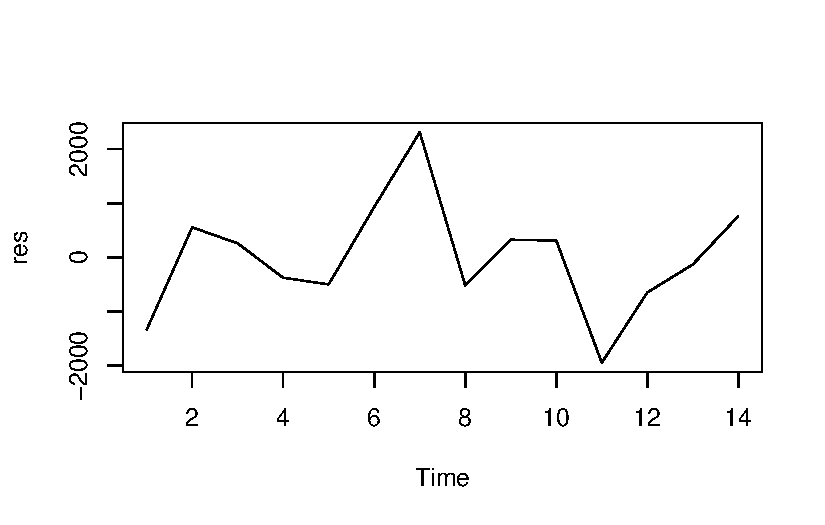
\includegraphics{tendencia_files/figure-pdf/unnamed-chunk-7-1.pdf}

}

\caption{Série dos resíduos}

}

\end{minipage}%
%
\begin{minipage}[t]{0.50\linewidth}

{\centering 

\raisebox{-\height}{

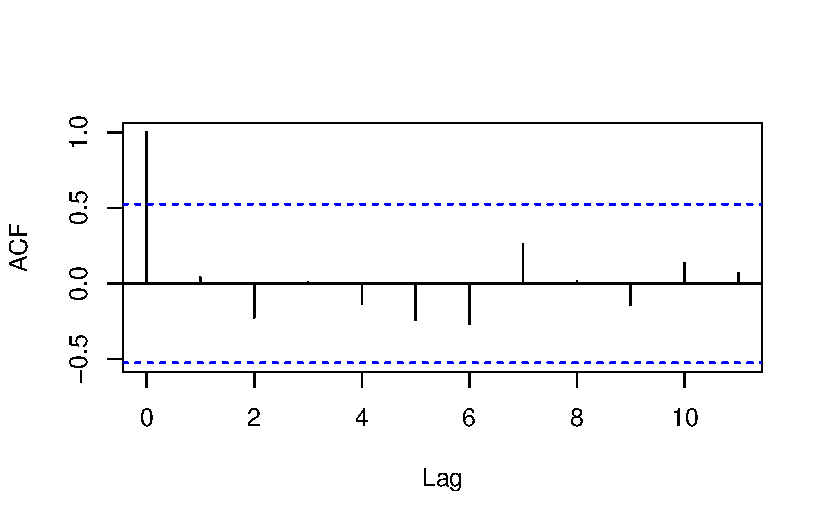
\includegraphics{tendencia_files/figure-pdf/unnamed-chunk-7-2.pdf}

}

\caption{Correlograma dos resíduos}

}

\end{minipage}%

\end{figure}

Abaixo, o teste de Shapiro-Wilks não gera evidências contra a suposição
de normalidade e o teste de Box-Pierce não gera evidências contra a
hipótese de ruído branco.

\begin{Shaded}
\begin{Highlighting}[]
\FunctionTok{shapiro.test}\NormalTok{(res)}
\end{Highlighting}
\end{Shaded}

\begin{verbatim}

    Shapiro-Wilk normality test

data:  res
W = 0.96982, p-value = 0.8743
\end{verbatim}

\begin{Shaded}
\begin{Highlighting}[]
\FunctionTok{Box.test}\NormalTok{(res)}
\end{Highlighting}
\end{Shaded}

\begin{verbatim}

    Box-Pierce test

data:  res
X-squared = 0.02156, df = 1, p-value = 0.8833
\end{verbatim}

É interessante notar que, para \(t=1,\ldots,14\),
\[\hat{T}(t)=\hat{\beta}_0+\hat{\beta}_1 t = \hat{y}_t,\] logo, os
valores preditos do modelo são uma estimativa para a tendência nos
pontos observados.

\begin{Shaded}
\begin{Highlighting}[]
\FunctionTok{ts.plot}\NormalTok{( }\FunctionTok{cbind}\NormalTok{( nascidos, }\FunctionTok{fitted}\NormalTok{(mod)), }\AttributeTok{col =} \DecValTok{1}\SpecialCharTok{:}\DecValTok{2}\NormalTok{, }\AttributeTok{lwd =} \DecValTok{2}\NormalTok{)}
\end{Highlighting}
\end{Shaded}

\begin{figure}

\begin{minipage}[t]{\linewidth}

{\centering 

\raisebox{-\height}{

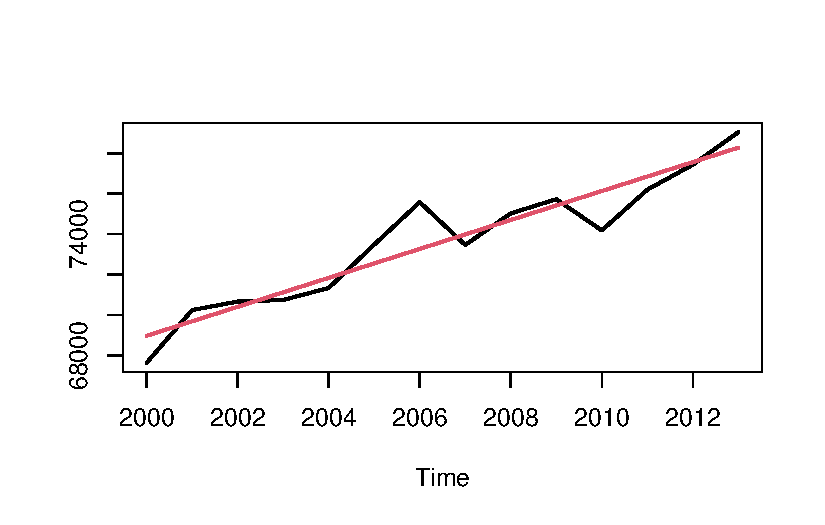
\includegraphics{tendencia_files/figure-pdf/unnamed-chunk-9-1.pdf}

}

\caption{Linha preta: série original. Linha vermelha: tendência
estimada}

}

\end{minipage}%

\end{figure}

\end{example}

\hypertarget{previsuxe3o}{%
\subsection{Previsão}\label{previsuxe3o}}

A previsão é realizada utilizando o modelo ajustado, estrapolando para
um tempo não observado. Por exemplo a estimativa para 2014 (\(t=15\)) é

\[\hat{T}(15)=\hat{\beta}+\hat{\beta}_1 15 = 78.992\] (o valor real foi
81.145).

É importante ressaltar que esse tipo de modelo é interessante para fazer
inferências sobre a tendência, mas pode ser inadequado para previsões,
uma vez que o polinômio é uma aproximação apenas para o intervalo
observado.

\hypertarget{seleuxe7uxe3o-de-modelos-lineares}{%
\subsection{Seleção de modelos
lineares}\label{seleuxe7uxe3o-de-modelos-lineares}}

O valor do Critério de Informação de Akaike (AIC) é dado por
\(-2L(\hat{\theta})+2k\) onde \(L\) é a função de verossimilhança e
\(\hat{\theta}\) e \(k\) são o estimador de máxima verossimilhança para
\(\theta\) e sua dimensão, respectivamente. O modelo com menor AIC é
considerado mais adequado.

Considere o nível anual, em pés, do Lago Huron. Essa série já vem
carregada no \texttt{R} sob o nome \texttt{LakeHuron}.

\begin{Shaded}
\begin{Highlighting}[]
\FunctionTok{ts.plot}\NormalTok{(LakeHuron, }\AttributeTok{lwd =} \DecValTok{2}\NormalTok{, }\AttributeTok{ylab =} \StringTok{\textquotesingle{}Nível (pés)\textquotesingle{}}\NormalTok{)}
\NormalTok{stats}\SpecialCharTok{::}\FunctionTok{acf}\NormalTok{(LakeHuron)}
\end{Highlighting}
\end{Shaded}

\begin{figure}

\begin{minipage}[t]{0.50\linewidth}

{\centering 

\raisebox{-\height}{

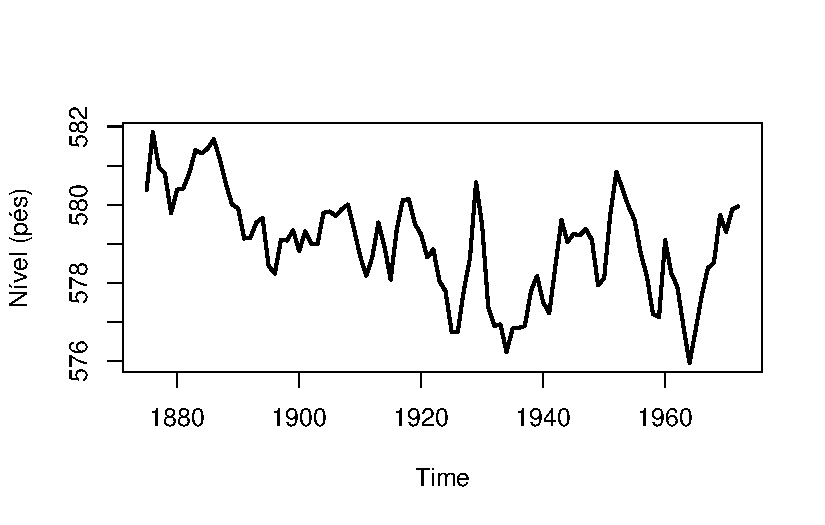
\includegraphics{tendencia_files/figure-pdf/fig-lakeHuron-1.pdf}

}

\caption{\label{fig-lakeHuron-1}Nível anual do Lago Huron, entre 1875 e
1972}

}

\end{minipage}%
%
\begin{minipage}[t]{0.50\linewidth}

{\centering 

\raisebox{-\height}{

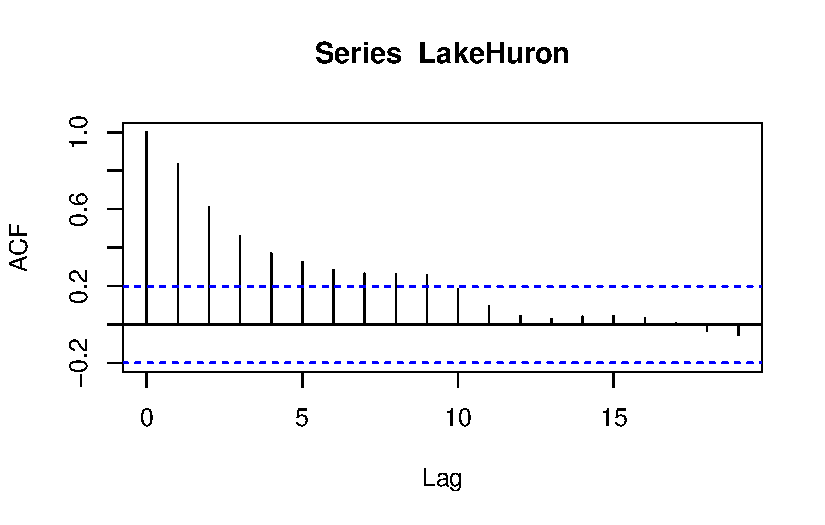
\includegraphics{tendencia_files/figure-pdf/fig-lakeHuron-2.pdf}

}

\caption{\label{fig-lakeHuron-2}Correlograma da série}

}

\end{minipage}%

\end{figure}

Vamos ajustar alguns modelos para tentar explica a tendêndia dessa
série.

\begin{Shaded}
\begin{Highlighting}[]
\NormalTok{tempo }\OtherTok{\textless{}{-}} \DecValTok{1} \SpecialCharTok{:} \FunctionTok{length}\NormalTok{(LakeHuron)}
\NormalTok{mod1 }\OtherTok{\textless{}{-}} \FunctionTok{lm}\NormalTok{( LakeHuron }\SpecialCharTok{\textasciitilde{}} \FunctionTok{poly}\NormalTok{(tempo, }\DecValTok{1}\NormalTok{, }\AttributeTok{raw =}\NormalTok{ T))}
\NormalTok{mod2 }\OtherTok{\textless{}{-}} \FunctionTok{lm}\NormalTok{( LakeHuron }\SpecialCharTok{\textasciitilde{}} \FunctionTok{poly}\NormalTok{(tempo, }\DecValTok{2}\NormalTok{, }\AttributeTok{raw =}\NormalTok{ T))}
\NormalTok{mod3 }\OtherTok{\textless{}{-}} \FunctionTok{lm}\NormalTok{( LakeHuron }\SpecialCharTok{\textasciitilde{}} \FunctionTok{poly}\NormalTok{(tempo, }\DecValTok{3}\NormalTok{, }\AttributeTok{raw =}\NormalTok{ T))}
\NormalTok{mod4 }\OtherTok{\textless{}{-}} \FunctionTok{lm}\NormalTok{( LakeHuron }\SpecialCharTok{\textasciitilde{}} \FunctionTok{poly}\NormalTok{(tempo, }\DecValTok{4}\NormalTok{, }\AttributeTok{raw =}\NormalTok{ T))}
\NormalTok{mod5 }\OtherTok{\textless{}{-}} \FunctionTok{lm}\NormalTok{( LakeHuron }\SpecialCharTok{\textasciitilde{}} \FunctionTok{poly}\NormalTok{(tempo, }\DecValTok{5}\NormalTok{, }\AttributeTok{raw =}\NormalTok{ T))}
\NormalTok{mod6 }\OtherTok{\textless{}{-}} \FunctionTok{lm}\NormalTok{( LakeHuron }\SpecialCharTok{\textasciitilde{}} \FunctionTok{poly}\NormalTok{(tempo, }\DecValTok{6}\NormalTok{, }\AttributeTok{raw =}\NormalTok{ T))}

\FunctionTok{AIC}\NormalTok{(mod1)}
\end{Highlighting}
\end{Shaded}

\begin{verbatim}
[1] 306.0957
\end{verbatim}

\begin{Shaded}
\begin{Highlighting}[]
\FunctionTok{AIC}\NormalTok{(mod2)}
\end{Highlighting}
\end{Shaded}

\begin{verbatim}
[1] 287.8407
\end{verbatim}

\begin{Shaded}
\begin{Highlighting}[]
\FunctionTok{AIC}\NormalTok{(mod3)}
\end{Highlighting}
\end{Shaded}

\begin{verbatim}
[1] 289.8391
\end{verbatim}

\begin{Shaded}
\begin{Highlighting}[]
\FunctionTok{AIC}\NormalTok{(mod4)}
\end{Highlighting}
\end{Shaded}

\begin{verbatim}
[1] 291.7127
\end{verbatim}

\begin{Shaded}
\begin{Highlighting}[]
\FunctionTok{AIC}\NormalTok{(mod5)}
\end{Highlighting}
\end{Shaded}

\begin{verbatim}
[1] 293.475
\end{verbatim}

\begin{Shaded}
\begin{Highlighting}[]
\FunctionTok{AIC}\NormalTok{(mod6)}
\end{Highlighting}
\end{Shaded}

\begin{verbatim}
[1] 291.7054
\end{verbatim}

Entre os modelos ajustados, o de ordem 2 foi aquele com o menor valor do
AIC. Sua tendência estimada é

O polinômio ajustado foi \[\hat{T}(t) = 581 -0,091 t + 0,001 t^2\]

Abaixo, apresentamos a análise de resíduos desse modelo.

\begin{Shaded}
\begin{Highlighting}[]
\NormalTok{res }\OtherTok{\textless{}{-}} \FunctionTok{residuals}\NormalTok{(mod2)}
\FunctionTok{ts.plot}\NormalTok{( res, }\AttributeTok{main =} \StringTok{\textquotesingle{}\textquotesingle{}}\NormalTok{)}
\FunctionTok{abline}\NormalTok{(}\AttributeTok{h =} \DecValTok{0}\NormalTok{, }\AttributeTok{lty =} \DecValTok{2}\NormalTok{)}
\FunctionTok{acf}\NormalTok{(res, }\AttributeTok{main =} \StringTok{\textquotesingle{}\textquotesingle{}}\NormalTok{)}
\end{Highlighting}
\end{Shaded}

\begin{figure}

\begin{minipage}[t]{0.50\linewidth}

{\centering 

\raisebox{-\height}{

\includegraphics{tendencia_files/figure-pdf/unnamed-chunk-12-1.pdf}

}

\caption{Série dos resíduos}

}

\end{minipage}%
%
\begin{minipage}[t]{0.50\linewidth}

{\centering 

\raisebox{-\height}{

\includegraphics{tendencia_files/figure-pdf/unnamed-chunk-12-2.pdf}

}

\caption{Correlograma dos resíduos}

}

\end{minipage}%

\end{figure}

Os resíduos parecem oscilar em torno de zero com um variância constante,
mas o correlograma sugere que não temos um ruído branco. O teste de
Box-Pierce, dado abaixo, confirma a nossa suspeita. Deste modo, este
modelo não é adequado.

\begin{Shaded}
\begin{Highlighting}[]
\FunctionTok{Box.test}\NormalTok{(res)}
\end{Highlighting}
\end{Shaded}

\begin{verbatim}

    Box-Pierce test

data:  res
X-squared = 50.973, df = 1, p-value = 9.365e-13
\end{verbatim}

\hypertarget{muxe9todos-nuxe3o-paramuxe9tricos-para-estimauxe7uxe3o-da-tenduxeancia}{%
\section{Métodos não paramétricos para estimação da
tendência}\label{muxe9todos-nuxe3o-paramuxe9tricos-para-estimauxe7uxe3o-da-tenduxeancia}}

O modelo de tendência polinomial é robusto quando relaxamos a
necessidade do ruído branco ser gaussiano. Nesse sentido, as estimativas
ainda são válidas, mas perdemos todos os testes de hipóteses.

Os métodos não paramétricos independem da distribuição do ruído, sendo
úteis para a análise exploratória.

\hypertarget{muxe9dias-muxf3veis}{%
\subsection{Médias Móveis}\label{muxe9dias-muxf3veis}}

O método das médias móveis consiste em obter \(\hat{T}(t)\) através da
média da série considerando os valores vizinhos à \(y_t\). Para o tempo
\(t\) e \(m=2h+1\), com \(h=1,2,\ldots\), considere o conjunto
\(\mathcal{V}(m)_t=\{t-h,\ldots,t+h\}\). Defini-se a média móvel de
ordem \(m\) (notamção \(m\)-MM) como
\[\hat{T}_h(t)=\frac{1}{m}\sum_{ i = t-h}^{t+h}y_i,\;h<t<n-h\].

Para compreender melhor esse estimador, considere que a relação entre
pontos vizinhos é aproximadamente linear, ou seja, para qualquer
\(t\in\mathcal{V}(m)_t\) existem \(a_\mathcal{V}\) e \(b_\mathcal{V}\)
tais que \[y_t\approx a_\mathcal{V}+b_\mathcal{V}t+\varepsilon_t,\] onde
\(\varepsilon_t\) é considerado uma série temporal estacionária e
ergódica. Então
\[\begin{align}E(\hat{T}(t))&=\frac{a_\mathcal{V}+b_\mathcal{V}(t-h)+\cdots+a_\mathcal{V}+b_\mathcal{V}t+\cdots+a_\mathcal{V}+b_\mathcal{V}(t+h)}{m}\\&=a_\mathcal{V}+b_\mathcal{V}t\end{align}\]
\[Var(\hat{T}(t))=\frac{\nu}{m}+\frac{2}{m}\sum_{j=1}^{2h}j\gamma(j)\]
Observe que, como \(T(.)\) é determinística e os ruídos são
estacionários e ergódicos, então \(Var(\hat{T}(t))\) converge para zero
quando \(m\rightarrow \infty\). Contudo, \(T(.)\) é localmente linear,
logo \(\hat{T}\) é um estimador razoável para valores baixos de \(h\).
Este é um exemplo típico de \emph{trade off} entre víes e variância,
onde não é possível minimizar os dois simultaneamente.

Utilizaremos a função \texttt{ma(x,m)}, do pacote \texttt{forecast} para
encontrar \(m-\)MM para a série `x

\begin{example}[]\protect\hypertarget{exm-NACIDOSMA}{}\label{exm-NACIDOSMA}

Abaixo, apresentamos a série anual histórica de nascidos vivos no
Amazonas desde 1994 até 2021.

\begin{Shaded}
\begin{Highlighting}[]
\NormalTok{x }\OtherTok{\textless{}{-}} \FunctionTok{c}\NormalTok{(}\DecValTok{47780}\NormalTok{, }\DecValTok{47966}\NormalTok{, }\DecValTok{49112}\NormalTok{, }\DecValTok{56070}\NormalTok{, }\DecValTok{57180}\NormalTok{, }\DecValTok{62037}\NormalTok{,}
\DecValTok{67646}\NormalTok{, }\DecValTok{70252}\NormalTok{, }\DecValTok{70671}\NormalTok{, }\DecValTok{70751}\NormalTok{, }\DecValTok{71345}\NormalTok{, }\DecValTok{73488}\NormalTok{, }\DecValTok{75584}\NormalTok{,}
\DecValTok{73469}\NormalTok{, }\DecValTok{75030}\NormalTok{, }\DecValTok{75729}\NormalTok{, }\DecValTok{74188}\NormalTok{, }\DecValTok{76202}\NormalTok{, }\DecValTok{77434}\NormalTok{, }\DecValTok{79041}\NormalTok{,}
\DecValTok{81145}\NormalTok{, }\DecValTok{80097}\NormalTok{, }\DecValTok{76703}\NormalTok{, }\DecValTok{78066}\NormalTok{, }\DecValTok{78087}\NormalTok{, }\DecValTok{77622}\NormalTok{, }\DecValTok{75635}\NormalTok{,}
\DecValTok{78454}\NormalTok{)}

\NormalTok{nascidos }\OtherTok{\textless{}{-}} \FunctionTok{ts}\NormalTok{(x, }\AttributeTok{start =}\DecValTok{1994}\NormalTok{)}
\FunctionTok{ts.plot}\NormalTok{(nascidos, }\AttributeTok{lwd =} \DecValTok{2}\NormalTok{, }\AttributeTok{ylab =} \StringTok{\textquotesingle{}No. nascidos vivos\textquotesingle{}}\NormalTok{)}
\end{Highlighting}
\end{Shaded}

\begin{figure}[H]

{\centering \includegraphics{tendencia_files/figure-pdf/unnamed-chunk-14-1.pdf}

}

\end{figure}

\begin{Shaded}
\begin{Highlighting}[]
\FunctionTok{require}\NormalTok{(forecast)}
\end{Highlighting}
\end{Shaded}

\begin{verbatim}
Carregando pacotes exigidos: forecast
\end{verbatim}

\begin{verbatim}
Warning: package 'forecast' was built under R version 4.3.1
\end{verbatim}

\begin{verbatim}
Registered S3 method overwritten by 'quantmod':
  method            from
  as.zoo.data.frame zoo 
\end{verbatim}

\begin{Shaded}
\begin{Highlighting}[]
\NormalTok{oo }\OtherTok{\textless{}{-}} \FunctionTok{par}\NormalTok{( }\AttributeTok{mfrow =} \FunctionTok{c}\NormalTok{(}\DecValTok{2}\NormalTok{,}\DecValTok{2}\NormalTok{), }\AttributeTok{mar =} \FunctionTok{c}\NormalTok{(}\DecValTok{2}\NormalTok{,}\DecValTok{2}\NormalTok{,}\DecValTok{1}\NormalTok{,}\DecValTok{1}\NormalTok{))}
\FunctionTok{ts.plot}\NormalTok{(nascidos, }\AttributeTok{lwd =} \DecValTok{2}\NormalTok{, }\AttributeTok{ylab =} \StringTok{\textquotesingle{}No. nascidos vivos\textquotesingle{}}\NormalTok{)}
\FunctionTok{lines}\NormalTok{( }\FunctionTok{ma}\NormalTok{(nascidos,}\DecValTok{3}\NormalTok{) , }\AttributeTok{col =}\DecValTok{2}\NormalTok{, }\AttributeTok{lwd =} \DecValTok{2}\NormalTok{)}
\FunctionTok{legend}\NormalTok{(}\StringTok{\textquotesingle{}bottomright\textquotesingle{}}\NormalTok{, }\AttributeTok{legend =} \FunctionTok{c}\NormalTok{(}\StringTok{\textquotesingle{}Série original\textquotesingle{}}\NormalTok{,}\StringTok{\textquotesingle{}3{-}MM\textquotesingle{}}\NormalTok{),  }\AttributeTok{fill =} \FunctionTok{c}\NormalTok{(}\DecValTok{1}\NormalTok{,}\DecValTok{2}\NormalTok{,}\DecValTok{3}\NormalTok{), }\AttributeTok{bty=}\StringTok{\textquotesingle{}n\textquotesingle{}}\NormalTok{)}
\FunctionTok{ts.plot}\NormalTok{(nascidos, }\AttributeTok{lwd =} \DecValTok{2}\NormalTok{, }\AttributeTok{ylab =} \StringTok{\textquotesingle{}No. nascidos vivos\textquotesingle{}}\NormalTok{)}
\FunctionTok{lines}\NormalTok{( }\FunctionTok{ma}\NormalTok{(nascidos,}\DecValTok{5}\NormalTok{) , }\AttributeTok{col =}\DecValTok{2}\NormalTok{, }\AttributeTok{lwd =} \DecValTok{2}\NormalTok{)}
\FunctionTok{legend}\NormalTok{(}\StringTok{\textquotesingle{}bottomright\textquotesingle{}}\NormalTok{, }\AttributeTok{legend =} \FunctionTok{c}\NormalTok{(}\StringTok{\textquotesingle{}Série original\textquotesingle{}}\NormalTok{,}\StringTok{\textquotesingle{}5{-}MM\textquotesingle{}}\NormalTok{),  }\AttributeTok{fill =} \FunctionTok{c}\NormalTok{(}\DecValTok{1}\NormalTok{,}\DecValTok{2}\NormalTok{,}\DecValTok{3}\NormalTok{), }\AttributeTok{bty=}\StringTok{\textquotesingle{}n\textquotesingle{}}\NormalTok{)}
\FunctionTok{ts.plot}\NormalTok{(nascidos, }\AttributeTok{lwd =} \DecValTok{2}\NormalTok{, }\AttributeTok{ylab =} \StringTok{\textquotesingle{}No. nascidos vivos\textquotesingle{}}\NormalTok{)}
\FunctionTok{lines}\NormalTok{( }\FunctionTok{ma}\NormalTok{(nascidos,}\DecValTok{7}\NormalTok{) , }\AttributeTok{col =}\DecValTok{2}\NormalTok{, }\AttributeTok{lwd =} \DecValTok{2}\NormalTok{)}
\FunctionTok{legend}\NormalTok{(}\StringTok{\textquotesingle{}bottomright\textquotesingle{}}\NormalTok{, }\AttributeTok{legend =} \FunctionTok{c}\NormalTok{(}\StringTok{\textquotesingle{}Série original\textquotesingle{}}\NormalTok{,}\StringTok{\textquotesingle{}7{-}MM\textquotesingle{}}\NormalTok{),  }\AttributeTok{fill =} \FunctionTok{c}\NormalTok{(}\DecValTok{1}\NormalTok{,}\DecValTok{2}\NormalTok{,}\DecValTok{3}\NormalTok{), }\AttributeTok{bty=}\StringTok{\textquotesingle{}n\textquotesingle{}}\NormalTok{)}
\FunctionTok{ts.plot}\NormalTok{(nascidos, }\AttributeTok{lwd =} \DecValTok{2}\NormalTok{, }\AttributeTok{ylab =} \StringTok{\textquotesingle{}No. nascidos vivos\textquotesingle{}}\NormalTok{)}
\FunctionTok{lines}\NormalTok{( }\FunctionTok{ma}\NormalTok{(nascidos,}\DecValTok{9}\NormalTok{) , }\AttributeTok{col =}\DecValTok{2}\NormalTok{, }\AttributeTok{lwd =} \DecValTok{2}\NormalTok{)}
\FunctionTok{legend}\NormalTok{(}\StringTok{\textquotesingle{}bottomright\textquotesingle{}}\NormalTok{, }\AttributeTok{legend =} \FunctionTok{c}\NormalTok{(}\StringTok{\textquotesingle{}Série original\textquotesingle{}}\NormalTok{,}\StringTok{\textquotesingle{}9{-}MM\textquotesingle{}}\NormalTok{),  }\AttributeTok{fill =} \FunctionTok{c}\NormalTok{(}\DecValTok{1}\NormalTok{,}\DecValTok{2}\NormalTok{,}\DecValTok{3}\NormalTok{), }\AttributeTok{bty=}\StringTok{\textquotesingle{}n\textquotesingle{}}\NormalTok{)}
\end{Highlighting}
\end{Shaded}

\begin{figure}[H]

{\centering 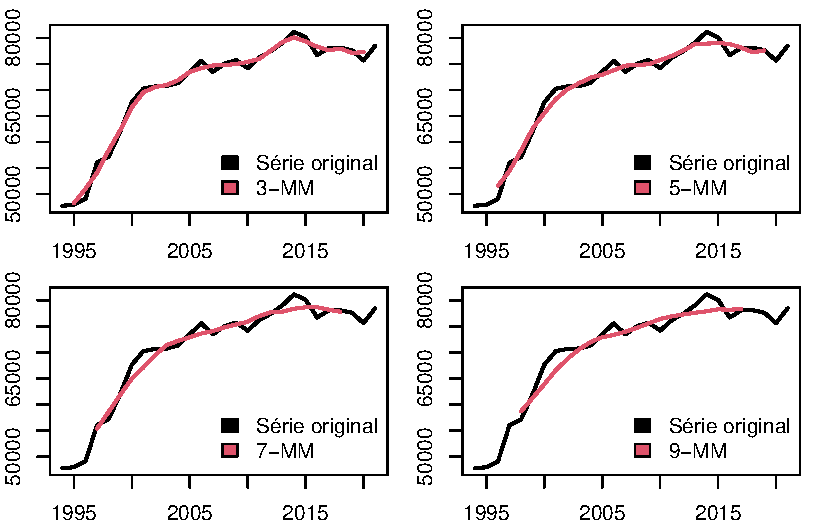
\includegraphics{tendencia_files/figure-pdf/unnamed-chunk-15-1.pdf}

}

\end{figure}

\begin{Shaded}
\begin{Highlighting}[]
\FunctionTok{par}\NormalTok{(oo)}
\end{Highlighting}
\end{Shaded}

Considere a estimativa obtida pela média móvel de ordem 3.

\begin{Shaded}
\begin{Highlighting}[]
\NormalTok{tendencia }\OtherTok{\textless{}{-}} \FunctionTok{ma}\NormalTok{(nascidos, }\DecValTok{3}\NormalTok{)}
\NormalTok{tendencia}
\end{Highlighting}
\end{Shaded}

\begin{verbatim}
Time Series:
Start = 1994 
End = 2021 
Frequency = 1 
 [1]       NA 48286.00 51049.33 54120.67 58429.00 62287.67 66645.00 69523.00
 [9] 70558.00 70922.33 71861.33 73472.33 74180.33 74694.33 74742.67 74982.33
[17] 75373.00 75941.33 77559.00 79206.67 80094.33 79315.00 78288.67 77618.67
[25] 77925.00 77114.67 77237.00       NA
\end{verbatim}

Vamos estimar o ruído da série (e eliminar as coordenadas vazias)

\begin{Shaded}
\begin{Highlighting}[]
\NormalTok{ruido }\OtherTok{\textless{}{-}}\NormalTok{ nascidos }\SpecialCharTok{{-}}\NormalTok{ tendencia}
\NormalTok{ruido }\OtherTok{\textless{}{-}}\NormalTok{ ruido[}\FunctionTok{is.na}\NormalTok{(ruido) }\SpecialCharTok{==}\NormalTok{ F]}
\end{Highlighting}
\end{Shaded}

Abaixo, apresentamos as principais estatísticas sobre os resíduos. A
série histórica dos resíduos oscila em torno de zero e não há motivos
para suspeitar de que sua variância é constante. O correlograma
apresenta autocorrelações baixas, como o esperado em um ruído branco. O
teste de Shapiro-Wilks não dá evidências contra normalidade, o que
suporta a hipótese de ruído branco gaussiano. O teste de Box-Pierce
apresenta um p-valor de 0,04 e, em conjunto com as demais evidências,
vamos considerá-lo significativo ao nível de 4\%.

\begin{Shaded}
\begin{Highlighting}[]
\FunctionTok{ts.plot}\NormalTok{(ruido)}
\FunctionTok{abline}\NormalTok{( }\AttributeTok{h =} \DecValTok{0}\NormalTok{, }\AttributeTok{lty =} \DecValTok{2}\NormalTok{)}
\FunctionTok{abline}\NormalTok{( }\AttributeTok{h =} \DecValTok{2}\SpecialCharTok{*}\FunctionTok{sd}\NormalTok{(ruido), }\AttributeTok{lty=}\DecValTok{2}\NormalTok{)}
\FunctionTok{abline}\NormalTok{( }\AttributeTok{h =} \SpecialCharTok{{-}}\DecValTok{2}\SpecialCharTok{*}\FunctionTok{sd}\NormalTok{(ruido), }\AttributeTok{lty=}\DecValTok{2}\NormalTok{)}
\end{Highlighting}
\end{Shaded}

\begin{figure}[H]

{\centering 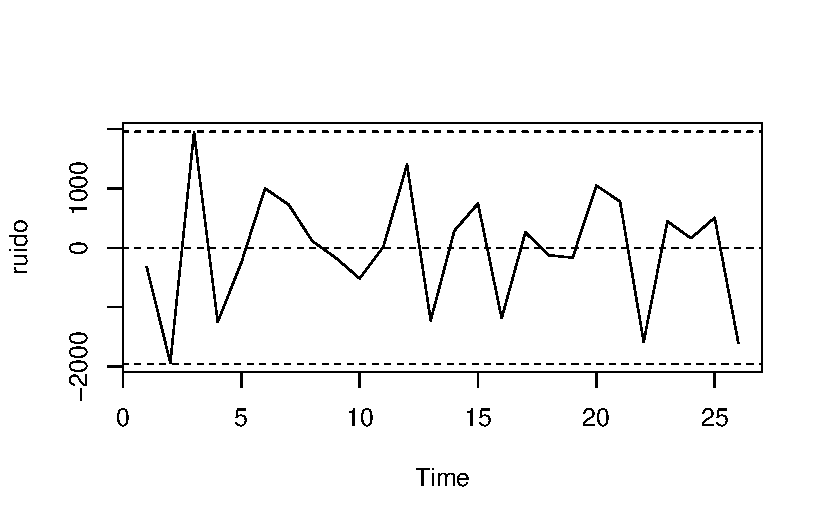
\includegraphics{tendencia_files/figure-pdf/unnamed-chunk-18-1.pdf}

}

\end{figure}

\begin{Shaded}
\begin{Highlighting}[]
\FunctionTok{acf}\NormalTok{(ruido)}
\end{Highlighting}
\end{Shaded}

\begin{figure}[H]

{\centering 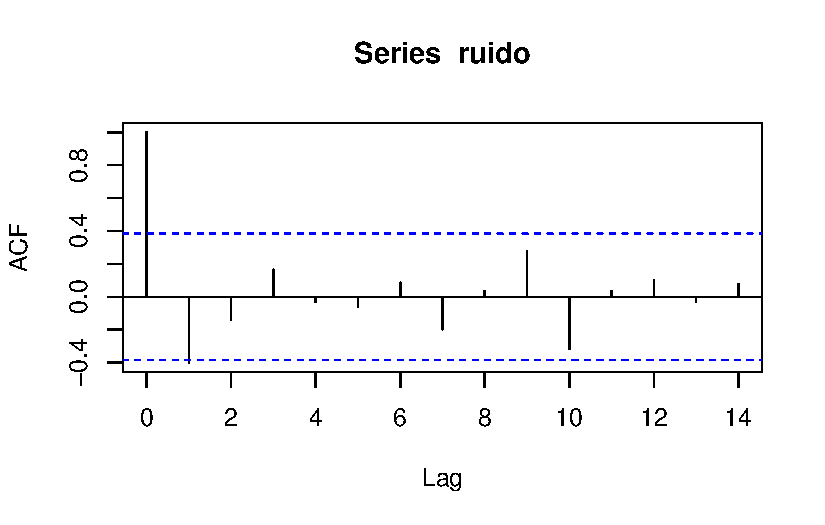
\includegraphics{tendencia_files/figure-pdf/unnamed-chunk-18-2.pdf}

}

\end{figure}

\begin{Shaded}
\begin{Highlighting}[]
\FunctionTok{shapiro.test}\NormalTok{(ruido)}
\end{Highlighting}
\end{Shaded}

\begin{verbatim}

    Shapiro-Wilk normality test

data:  ruido
W = 0.9711, p-value = 0.6521
\end{verbatim}

\begin{Shaded}
\begin{Highlighting}[]
\FunctionTok{Box.test}\NormalTok{(ruido)}
\end{Highlighting}
\end{Shaded}

\begin{verbatim}

    Box-Pierce test

data:  ruido
X-squared = 4.1804, df = 1, p-value = 0.04089
\end{verbatim}

\(\blacksquare\)

\end{example}

Até o momento, foi considerado que a ordem da média móvel é escrita como
\(m=2h+1\), ou seja, a ordem é sempre ímpar. Sem Para definir a média
móvel para uma ordem par, perda de generalidade, assuma que \(m=4\).
Como não é possível escolher um número igual de vizinhos à \(y_t\),
tem-se duas possibilidades para \(\mathcal{V}(4)_t\):
\[\mathcal{V}'(4)_t=\{y_{t-1},y_t,y_{t+1},y_{t+2}\}\] e
\[\mathcal{V}''(4)_t=\{y_{t-2},y_{t-1},y_t,y_{t+1}\}.\] Para cada
possibilidade, tem-se \[\hat{T}'(t)=\frac{1}{4}\sum_{i=t-1}^{t+2}y_{i}\]
e \[\hat{T}''(t)=\frac{1}{4}\sum_{i=t-2}^{t+1}y_{i}.\] A média móvel
2-MM será definida por \[\hat{T}(t)=\frac{T'(t)+T''(t)}{2}\] Observe que
a média agora é ponderada, uma vez que

\[\hat{T}(t)=\frac{y_{t-2}}{8}+\frac{y_{t-1}}{4}+\frac{y_{t}}{4}+\frac{y_{t+1}}{4}+\frac{y_{t+2}}{8}.\]

Para o caso de \(m=2h\) com \(h=1,2,\ldots\), defini-se \(m\)-MM por
\[\begin{align}\hat{T}(t)&=\frac{1}{2}\left[\frac{1}{m}\sum_{i=t-h}^{t+h-1}y_i+\frac{1}{m}\sum_{i=t-h+1}^{t+h}y_i\right]\\&=\frac{y_{t-h}}{2m}+\frac{1}{m}\sum_{i=t-h+1}^{t+h-1}y_i+\frac{y_{t+h}}{2m}.\end{align}\]
Note que o argumento de \(\hat{T}(t)\) é aproximadamente não viciado
para \(m\) pequeno não se altera, uma vez que os pesos para os tempos
\(t-j\) e \(t+j\) são simétricos

O estimador para tendência conhecido como média móvel ponderada de ordem
\(m\) é dado por

\[\hat{T}(t)=\sum_{i=t-h}^{t+h} w_i y_{i},\] com \(w_i>0\),
\(w_{t-j}=w_{t+j}\) e \(\sum_{i=t-h}^{t+h}w_i=1\). O método tradicional
é obtido fazendo \(w_i=1/m\).

Por último, como as primeiras e últimas observações são removidas, esses
métodos não são os mais recomendados.

\textbf{Outras médias móveis}

É importante ressaltar que os métodos estatísticos são ferramentas
universais e que geralmente sofrem modificações ao serem aplicados em
outras áreas. Deste modo, existem outras definições de médias móveis que
podem causar confusão.

Em epidemiologia por exemplo, a média móvel de ordem \(m\) é definida
por \[\hat{T}(t)=\frac{1}{m}\sum_{j=1}^m y_{t-j+1}\] ou seja, a soma dos
valores mais recentes em relação à \(t\). Observe que o contexto é
diferente: em uma epidemia por exemplo, deseja-se estimar \(T(t)\) onde
\(t\) é o tempo mais recente e, em geral, se utiliza o 7-MM tirando a
média dos últimos 7 dias. A mesma lógica vale para o mercado financeiro,
que tira a média dos últimos 5 dias de preço de fechamento.

Ainda no mercado financeiro, o importante é captar a mudança da
tendência o mais rápido possível. Deste modo, utiliza-se uma média móvel
ponderada definida por
\[\hat{T}(t)=\frac{2}{m(m+1)}\sum_{j=1}^m(m-j+1)y_{t-j+1}.\] Na
definição acima, o último preço da ação, dado por \(y_t\), é o valor
mais imporante e por isso recebe o maior peso. Note que os pesos não são
simétricos.

\hypertarget{suavizauxe7uxe3o-do-gruxe1fico-de-dispersuxe3o-estimada-localmente-loess}{%
\section{Suavização do gráfico de dispersão estimada localmente
(loess)}\label{suavizauxe7uxe3o-do-gruxe1fico-de-dispersuxe3o-estimada-localmente-loess}}

No método de suavisação do gráfico de dispersão, deseja-se estimar
\(f(x)=E(y|x)\), através da coleção \((y_1,x_1),\ldots,(y_n,x_n)\), para
um valor qualquer de \(x\).

A estimativa \(\hat{f}\) para o ponto \(x'\) é calculada considerando os
seguintes passos:

\begin{enumerate}
\def\labelenumi{\arabic{enumi}.}
\item
  Fixe um valor inteiro positivo \(q\leq n\).
\item
  Dentro do conjunto \(x_1,\ldots,x_n,\) encontre os \(q\) valores mais
  próximos de \(x'\) (via distância euclidiana). Denote este conjunto
  por \(\mathcal{V}\) e denote por \(d\) a maior distância encontrada.
\item
  Para cada \(x_1,\ldots,x_n\) seja
  \[v_j(x')=\left\{\begin{array}{ll}\left(1-\left| \frac{x_j-x'}{d}\right|^3\right)^3&,\;\;\hbox{se }|x_j-x|\leq d\\ 0,&\hbox{caso contrário}\end{array}\right.\]
  o peso associado à \(x_j\) (valores próximos de \(x'\) receberão o
  peso máximo e valores afastados recebem menor peso)
\item
  Ajuste o modelo de regressão ponderado, minimizando
  \[\sum_{i=1}^n v_i(x')\left(y_i - \sum_{j=0}^p \beta_jx^j\right)^2\]
\item
  Estime \(f(x')\) por \[\hat{f}(x')=\sum_{j=0}^p \hat{\beta}_jx^j \]
\end{enumerate}

Oberve que este método pode ser utilizado para estimar a tendência da
série. Abaixo, vamos analisar a série de taxa de desemprego mensal,
entre março de 2002 e dezembro de 2015.

\begin{Shaded}
\begin{Highlighting}[]
\NormalTok{url }\OtherTok{\textless{}{-}} \StringTok{\textquotesingle{}https://www.dropbox.com/s/rmgymzsic99qawd/desemprego.csv?dl=1\textquotesingle{}}

\NormalTok{banco }\OtherTok{\textless{}{-}} \FunctionTok{read.csv}\NormalTok{(url, }\AttributeTok{sep =} \StringTok{\textquotesingle{};\textquotesingle{}}\NormalTok{, }\AttributeTok{h =}\NormalTok{ F)}

\NormalTok{desemprego}\OtherTok{\textless{}{-}} \FunctionTok{ts}\NormalTok{( banco}\SpecialCharTok{$}\NormalTok{V2, }\AttributeTok{start =} \FunctionTok{c}\NormalTok{(}\DecValTok{2002}\NormalTok{,}\DecValTok{3}\NormalTok{), }\AttributeTok{frequency=}\DecValTok{12}\NormalTok{)}

\FunctionTok{ts.plot}\NormalTok{(desemprego, }\AttributeTok{ylab =} \StringTok{\textquotesingle{}Taxa de desemprego\textquotesingle{}}\NormalTok{)}
\end{Highlighting}
\end{Shaded}

\begin{figure}[H]

{\centering 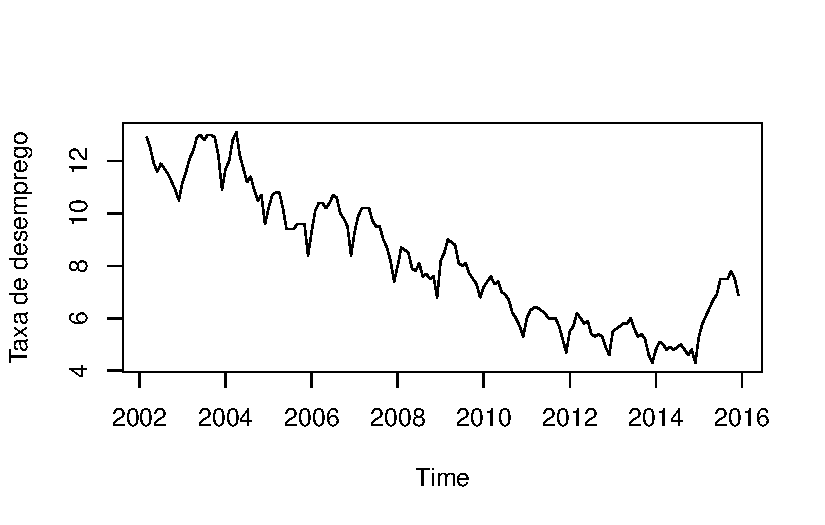
\includegraphics{tendencia_files/figure-pdf/unnamed-chunk-19-1.pdf}

}

\end{figure}

\begin{Shaded}
\begin{Highlighting}[]
\FunctionTok{acf}\NormalTok{(desemprego, }\AttributeTok{lag =} \DecValTok{30}\NormalTok{)}
\end{Highlighting}
\end{Shaded}

\begin{figure}[H]

{\centering 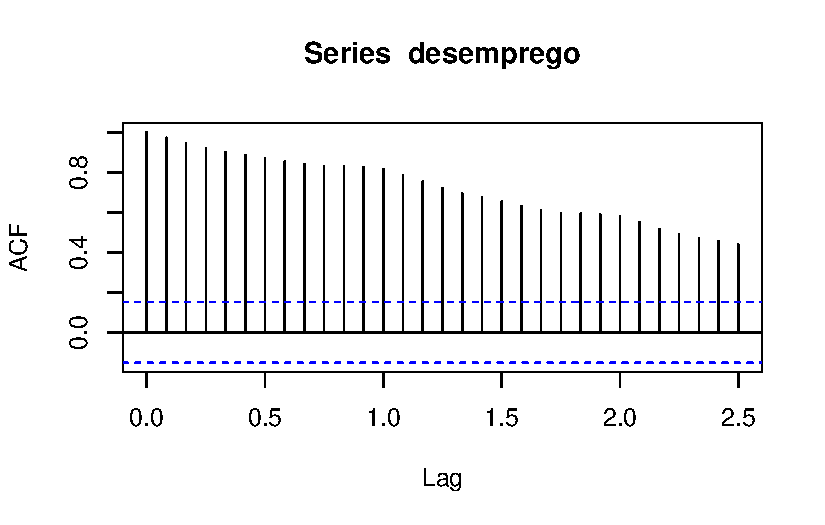
\includegraphics{tendencia_files/figure-pdf/unnamed-chunk-19-2.pdf}

}

\end{figure}

Vamos estimar a tendência

\begin{Shaded}
\begin{Highlighting}[]
\CommentTok{\# criando a variável regressora}
\NormalTok{tempo }\OtherTok{\textless{}{-}} \DecValTok{1} \SpecialCharTok{:} \FunctionTok{length}\NormalTok{(desemprego)}

\CommentTok{\# aplicando o loess}
\NormalTok{lw }\OtherTok{\textless{}{-}} \FunctionTok{loess}\NormalTok{( desemprego }\SpecialCharTok{\textasciitilde{}}\NormalTok{ tempo)}

\CommentTok{\# transformando o valor predito em uma série temporal}

\NormalTok{fit }\OtherTok{\textless{}{-}} \FunctionTok{ts}\NormalTok{(lw}\SpecialCharTok{$}\NormalTok{fitted, }\AttributeTok{start =} \FunctionTok{start}\NormalTok{(desemprego), }\AttributeTok{frequency =} \FunctionTok{frequency}\NormalTok{(desemprego) )}

\CommentTok{\# gráfico da tendência estimada}

\FunctionTok{ts.plot}\NormalTok{( desemprego, }\AttributeTok{ylab =} \StringTok{\textquotesingle{}Taxa de desemprego\textquotesingle{}}\NormalTok{ , }\AttributeTok{lwd =} \DecValTok{2}\NormalTok{)}
\FunctionTok{lines}\NormalTok{(fit, }\AttributeTok{lwd =} \DecValTok{2}\NormalTok{, }\AttributeTok{col =} \StringTok{\textquotesingle{}tomato\textquotesingle{}}\NormalTok{)}
\FunctionTok{legend}\NormalTok{(}\StringTok{\textquotesingle{}topright\textquotesingle{}}\NormalTok{, }\FunctionTok{c}\NormalTok{(}\StringTok{\textquotesingle{}Observado\textquotesingle{}}\NormalTok{,}\StringTok{\textquotesingle{}Ajustado\textquotesingle{}}\NormalTok{),}\AttributeTok{fill=}\FunctionTok{c}\NormalTok{(}\DecValTok{1}\NormalTok{,}\StringTok{\textquotesingle{}tomato\textquotesingle{}}\NormalTok{), }\AttributeTok{bty=}\StringTok{\textquotesingle{}n\textquotesingle{}}\NormalTok{)}
\end{Highlighting}
\end{Shaded}

\begin{figure}[H]

{\centering 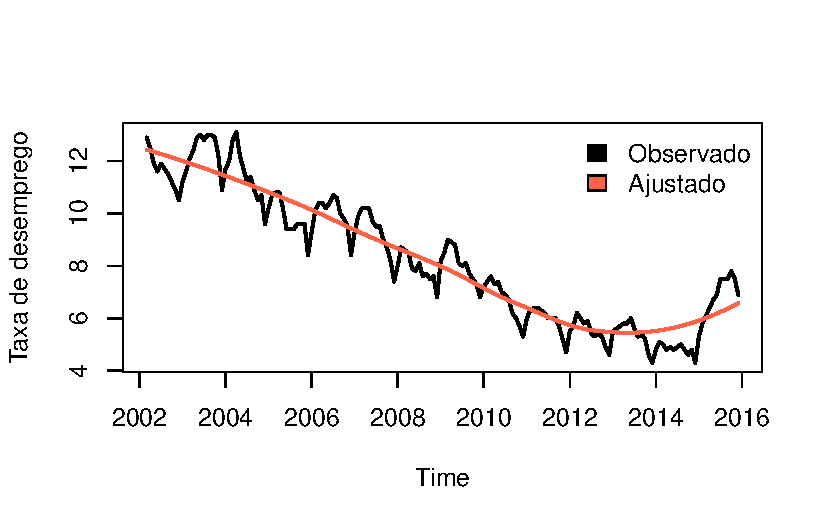
\includegraphics{tendencia_files/figure-pdf/unnamed-chunk-20-1.pdf}

}

\end{figure}

Vamos eliminar a tendência estimada e avaliar o restante.

\begin{Shaded}
\begin{Highlighting}[]
\NormalTok{yt }\OtherTok{\textless{}{-}}\NormalTok{ desemprego }\SpecialCharTok{{-}}\NormalTok{ fit}

\FunctionTok{ts.plot}\NormalTok{(yt)}
\end{Highlighting}
\end{Shaded}

\begin{figure}[H]

{\centering 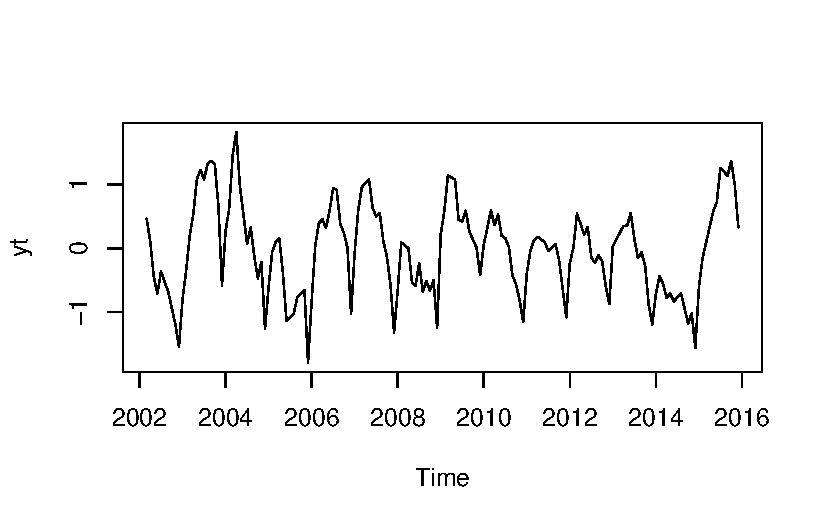
\includegraphics{tendencia_files/figure-pdf/unnamed-chunk-21-1.pdf}

}

\end{figure}

\begin{Shaded}
\begin{Highlighting}[]
\FunctionTok{acf}\NormalTok{(yt)}
\end{Highlighting}
\end{Shaded}

\begin{figure}[H]

{\centering 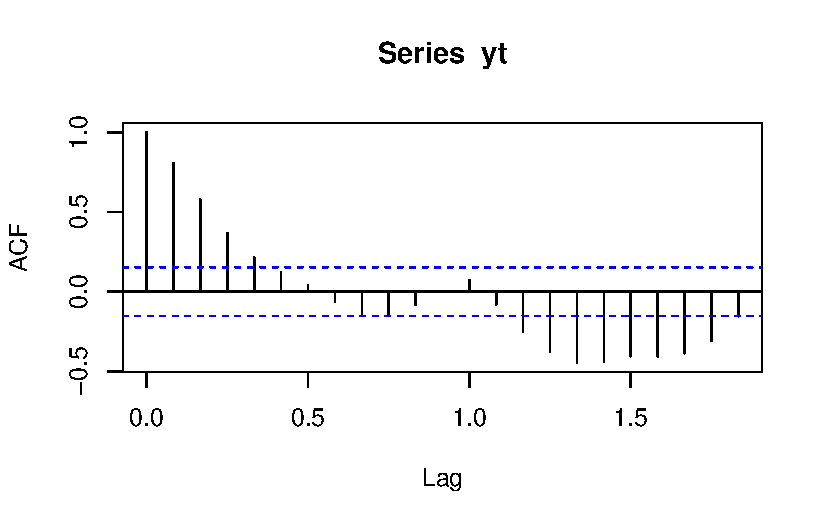
\includegraphics{tendencia_files/figure-pdf/unnamed-chunk-21-2.pdf}

}

\end{figure}

Fica claro o comportamento sazonal, o que implica que o restante não é
uma série estacionária.

\bookmarksetup{startatroot}

\hypertarget{sazonalidade}{%
\chapter{Sazonalidade}\label{sazonalidade}}

\hypertarget{padruxe3o-sazonal}{%
\section{Padrão sazonal}\label{padruxe3o-sazonal}}

Padrões que surgem sistematicamente ao longo do tempo são denominados
sazonais. Exemplos: flutuações de temperatura entre estações, início e
fim do semestre letivo, Natal, dias úteis, feriados flutuantes como a
Páscoa e o Carnaval.

Um padrão sazonal pode ser modelado através de uma função periódica.

\begin{definition}[]\protect\hypertarget{def-periodica}{}\label{def-periodica}

Dizemos que \(s(.)\) é uma função periódica de período \(p\) se
\[s(t)=s(t + kp),\;\forall k=1,2,\ldots.\]

\end{definition}

\begin{example}[]\protect\hypertarget{exm-periodica}{}\label{exm-periodica}

A função \[s(t)=\left\{ \begin{align}
-1, &\;\;t=1,4,7,\ldots\\
0, &\;\; t=2,5,8,\ldots\\
1,&\;\;t=3,6,9,\ldots
\end{align}
\right.
\] é periódica e possui período \(p=3\).

\end{example}

\begin{example}[]\protect\hypertarget{exm-periodica2}{}\label{exm-periodica2}

A função \[s(t)=\cos\left(2\pi\frac{t}{4}\right)\] é periódica (com
\(p=4\)). De fato, para \(k=1,2,3,\ldots,\) \[\begin{align*}
    g(t+4k) &= \cos\left(2\pi\frac{t+4k}{4}\right)=\cos\left( \pi\frac{t}{4}+2\pi k\right)\\
    &=\cos\left( 2\pi\frac{t}{4}\right)\underbrace{\cos\left(2\pi k\right)}_\text{1} - \sin\left( \pi\frac{t}{4}\right)\underbrace{\sin\left(2\pi k\right)}_\text{0}\\
    &=\cos\left(2\pi\frac{t}{4}\right) = g(t).  
\end{align*}\]

\end{example}

Seja \(s(.)\) uma função periódica. Então, uma série temporal sazonal
aditiva é descrita como

\[x_t=s(t)+\varepsilon_t,\] onde \(\varepsilon_t\) é um ruído
estacionário.

\textbf{Atenção.} Ao criar um objeto do tipo \texttt{ts} no \texttt{R},
o argumento \texttt{frequency} é considerado o período do padrão
sazonal. A maioria das funções voltadas para padrões sazonais acessam
essa informação no objeto.

\hypertarget{gruxe1ficos-sazonal-de-subsuxe9ries}{%
\section{Gráficos sazonal de
subséries}\label{gruxe1ficos-sazonal-de-subsuxe9ries}}

Seja \(x_t\) uma série sazonal de período \(p\). Para construir um
gráfico sazonal de subséries:

\begin{itemize}
\item
  Faça \(p\) subséries: \[\begin{align*}
        &x_1,x_{1+p},x_{1+2p},\ldots \\
        &x_{2},x_{2+p},x_{2+2p},\ldots\\
        &\cdots\\
        &x_{p},x_{2p},x_{3p},\ldots\\       
        \end{align*}\]
\item
  Calcule a média de cada subsérie.
\item
  Faça um gráfico de cada subsérie, cada um com uma linha horizontal com
  o valor de sua respectiva média.
\end{itemize}

Observe que, para um padrão sazonal, a subsérie
\[x_{i},x_{i+p},x_{i+2p},\ldots\] é equivalente à
\[s(i)+\varepsilon_i,s(i)+\varepsilon_{i+p},s(i)+\varepsilon_{i+2p},\ldots\]
e, supondo que \(\varepsilon_t\) é um ruído granco ergódico, teremos que
\[\hat{s}(i)=\frac{1}{m+1}\sum_{j=0}^m x_{i+jp}\] onde \(m+1\) é o
tamanho da amostra correspodente à subsérie.

No \texttt{R}, o comando \texttt{monthplot(x)} faz o gráfico de
subséries. Considerando um padrão sazonal, cada subsérie deve oscilar em
torno de uma média constante. Vejamos algus exemplos.

\begin{example}[]\protect\hypertarget{exm-nottem1}{}\label{exm-nottem1}

A série abaixo (gráfico à esquerda) apresenta as temperaturas médias
mensais, em Fahrenheits, no Castelo de Nottingham entre 1920 e 1939. O
gráfico à direita apresenta o gráfico de subséries. Como a série possui
período 12, este último gráfico já identifica cada subsérie com a
inicial do mês correspondente. Note que a maioria das subséries oscila
em torno da média

\begin{Shaded}
\begin{Highlighting}[]
\FunctionTok{ts.plot}\NormalTok{(nottem)}
\FunctionTok{monthplot}\NormalTok{(nottem)}
\end{Highlighting}
\end{Shaded}

\begin{figure}

\begin{minipage}[t]{0.50\linewidth}

{\centering 

\raisebox{-\height}{

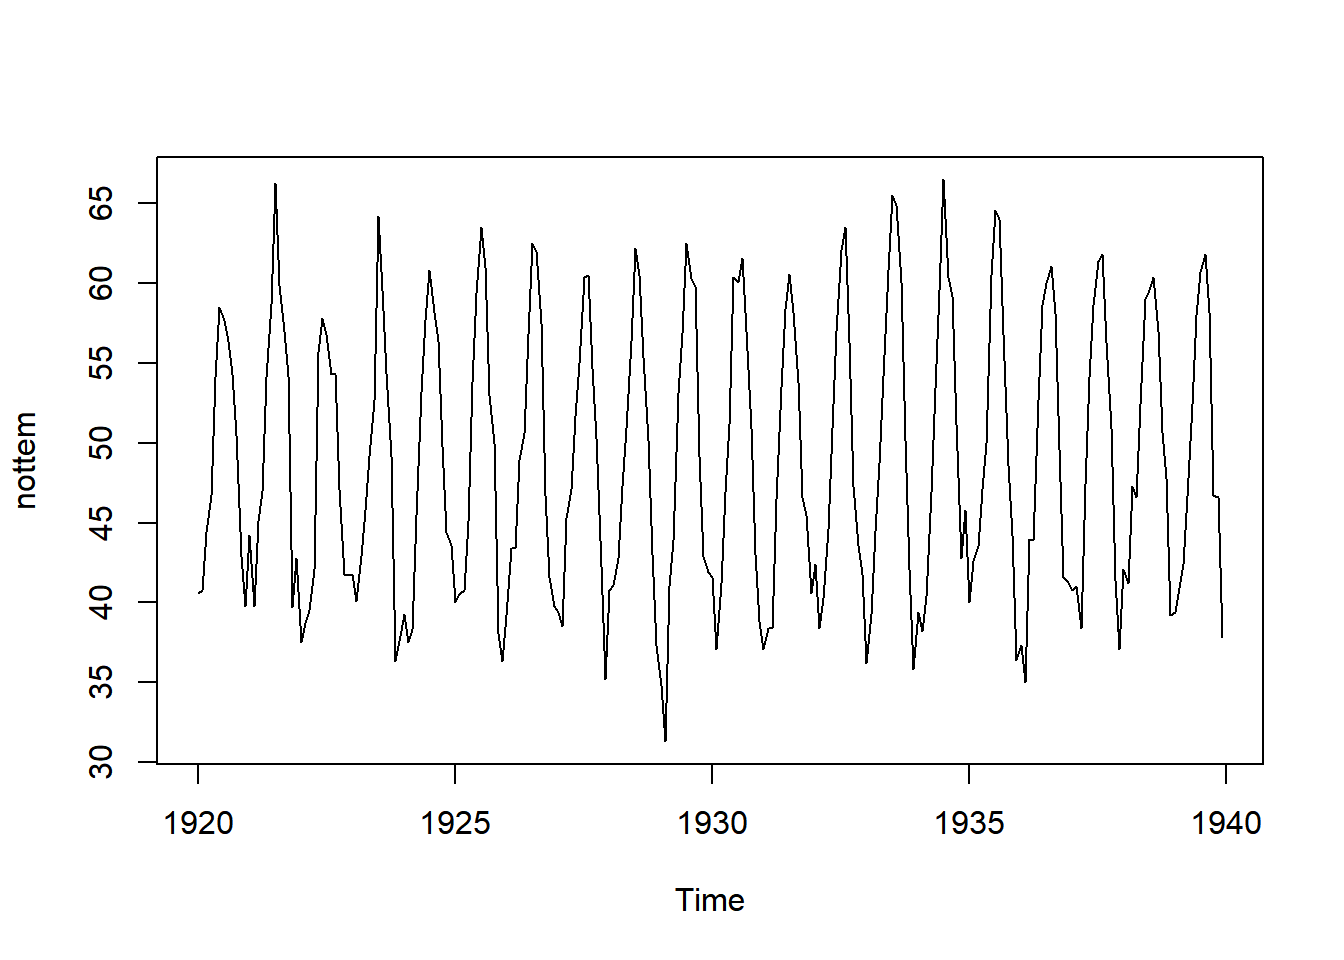
\includegraphics{sazonalidade_files/figure-pdf/fig-nottemMonthplot-1.pdf}

}

\caption{\label{fig-nottemMonthplot-1}Gráfico da série de temperaturas
no Castelo de Nottingham}

}

\end{minipage}%
%
\begin{minipage}[t]{0.50\linewidth}

{\centering 

\raisebox{-\height}{

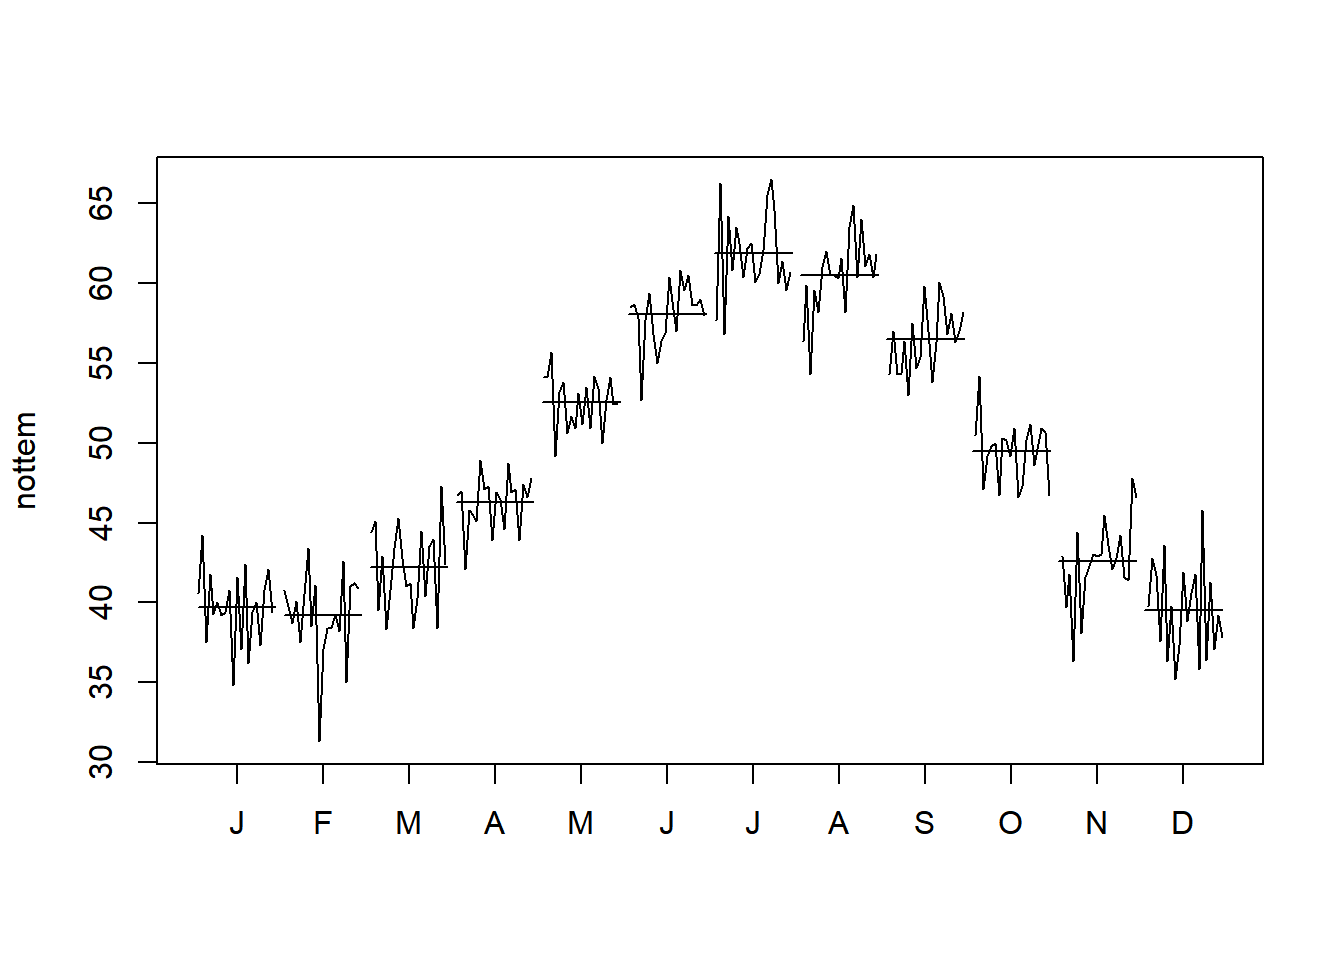
\includegraphics{sazonalidade_files/figure-pdf/fig-nottemMonthplot-2.pdf}

}

\caption{\label{fig-nottemMonthplot-2}Gráfico de subséries}

}

\end{minipage}%

\end{figure}

\(\blacksquare\)

\end{example}

É possível que a tendência construa uma falta impressão sobre o
comportamento sazonal. Portanto, é interessante remover a tendência da
série antes de fazer o gráfico das subséries.

\begin{example}[]\protect\hypertarget{exm-co2Monthoplot}{}\label{exm-co2Monthoplot}

Abaixo apresentamos a série mensal da concentração de CO\(_2\), em
partes por milhão, no Mauna Loa. Observe a clara tendência de
crescimento e o padrão sazonal.

\begin{Shaded}
\begin{Highlighting}[]
\FunctionTok{ts.plot}\NormalTok{(co2)}
\end{Highlighting}
\end{Shaded}

\begin{figure}[H]

{\centering \includegraphics{sazonalidade_files/figure-pdf/unnamed-chunk-2-1.pdf}

}

\end{figure}

O gráfico das subséries é dado abaixo. Observe que há uma tendência
crescente em cada subsérie.

\begin{Shaded}
\begin{Highlighting}[]
\FunctionTok{monthplot}\NormalTok{(co2)}
\end{Highlighting}
\end{Shaded}

\begin{figure}[H]

{\centering \includegraphics{sazonalidade_files/figure-pdf/unnamed-chunk-3-1.pdf}

}

\end{figure}

A tendência crescente nas subséries não nos nos permitiria trabalhar com
uma função periódica. Contudo o gráfico está sendo influenciado pela
tendência. Vamos removê-la e fazer o gráfico novamente.

\begin{Shaded}
\begin{Highlighting}[]
\CommentTok{\# estimação da tendência via loess}
\NormalTok{tempo }\OtherTok{\textless{}{-}} \DecValTok{1} \SpecialCharTok{:} \FunctionTok{length}\NormalTok{(co2)}
\NormalTok{model }\OtherTok{\textless{}{-}} \FunctionTok{loess}\NormalTok{( co2 }\SpecialCharTok{\textasciitilde{}}\NormalTok{tempo)}
\NormalTok{tend }\OtherTok{\textless{}{-}} \FunctionTok{fitted}\NormalTok{(model)}

\CommentTok{\# série sem tendência e o gráfico de subséries}
\FunctionTok{plot}\NormalTok{( co2}\SpecialCharTok{{-}}\NormalTok{tend)}
\end{Highlighting}
\end{Shaded}

\begin{figure}[H]

{\centering \includegraphics{sazonalidade_files/figure-pdf/unnamed-chunk-4-1.pdf}

}

\end{figure}

\begin{Shaded}
\begin{Highlighting}[]
\FunctionTok{monthplot}\NormalTok{(co2}\SpecialCharTok{{-}}\NormalTok{tend)}
\end{Highlighting}
\end{Shaded}

\begin{figure}[H]

{\centering 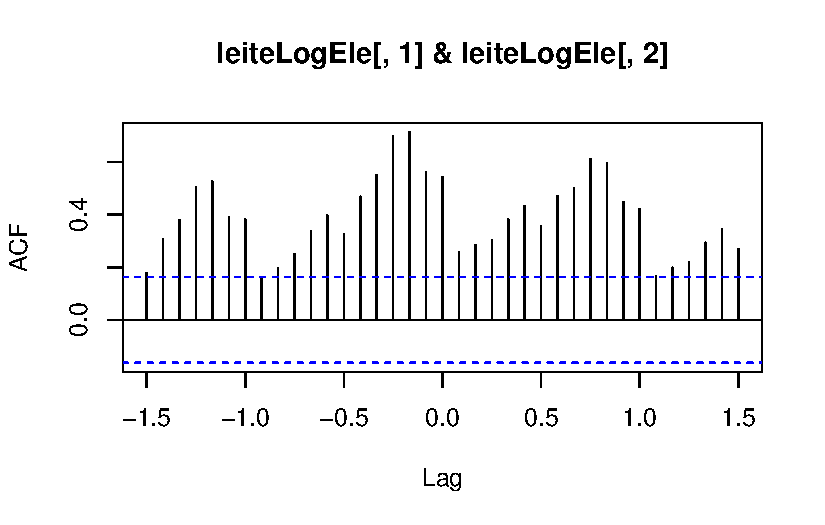
\includegraphics{sazonalidade_files/figure-pdf/unnamed-chunk-4-2.pdf}

}

\end{figure}

\(\blacksquare\)

\end{example}

Também é possível que o padrão sazonal não seja bem representado por uma
função periódica. Isto ocorre quando o gráfico de subséries possui
tendência.

\begin{example}[]\protect\hypertarget{exm-AirPassengersMonthplot}{}\label{exm-AirPassengersMonthplot}

A \textbf{?@fig-AirPassengersMonthplot} apresenta o gráfico da série
\texttt{AirPassengers} e de suas subséries. Observe que todas as
subséries possuem um padrão de crescimento, que deve estar sendo
governado pela tendência crescente da série.

\begin{Shaded}
\begin{Highlighting}[]
\FunctionTok{ts.plot}\NormalTok{(AirPassengers)}
\FunctionTok{monthplot}\NormalTok{(AirPassengers)}
\end{Highlighting}
\end{Shaded}

\begin{figure}

\begin{minipage}[t]{0.50\linewidth}

{\centering 

\raisebox{-\height}{

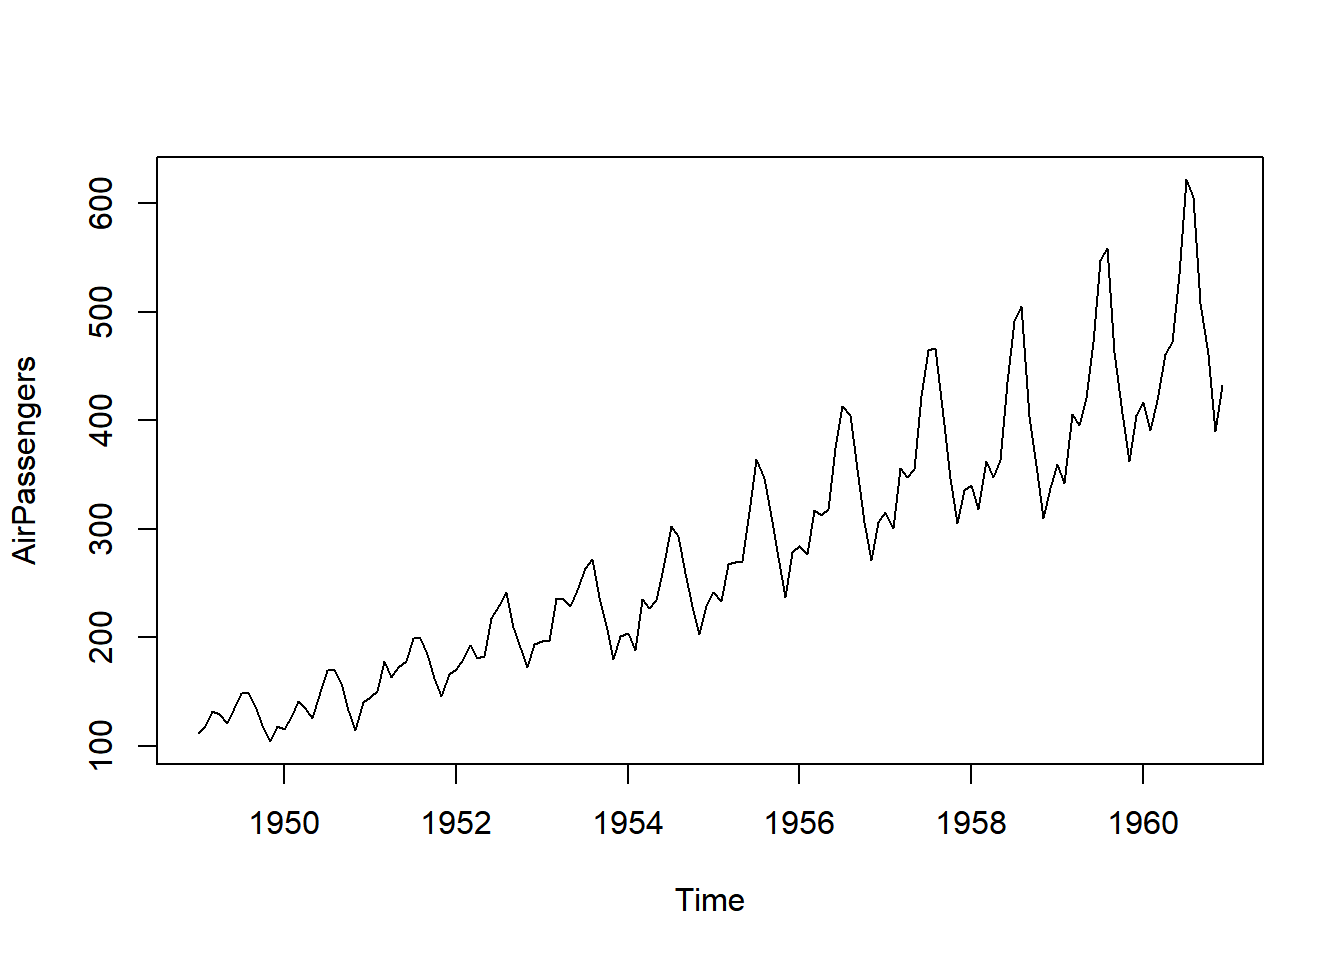
\includegraphics{sazonalidade_files/figure-pdf/fig-AirPassengersMonthplot-1.pdf}

}

\caption{\label{fig-AirPassengersMonthplot-1}Gráfico da série
AirPassengers}

}

\end{minipage}%
%
\begin{minipage}[t]{0.50\linewidth}

{\centering 

\raisebox{-\height}{

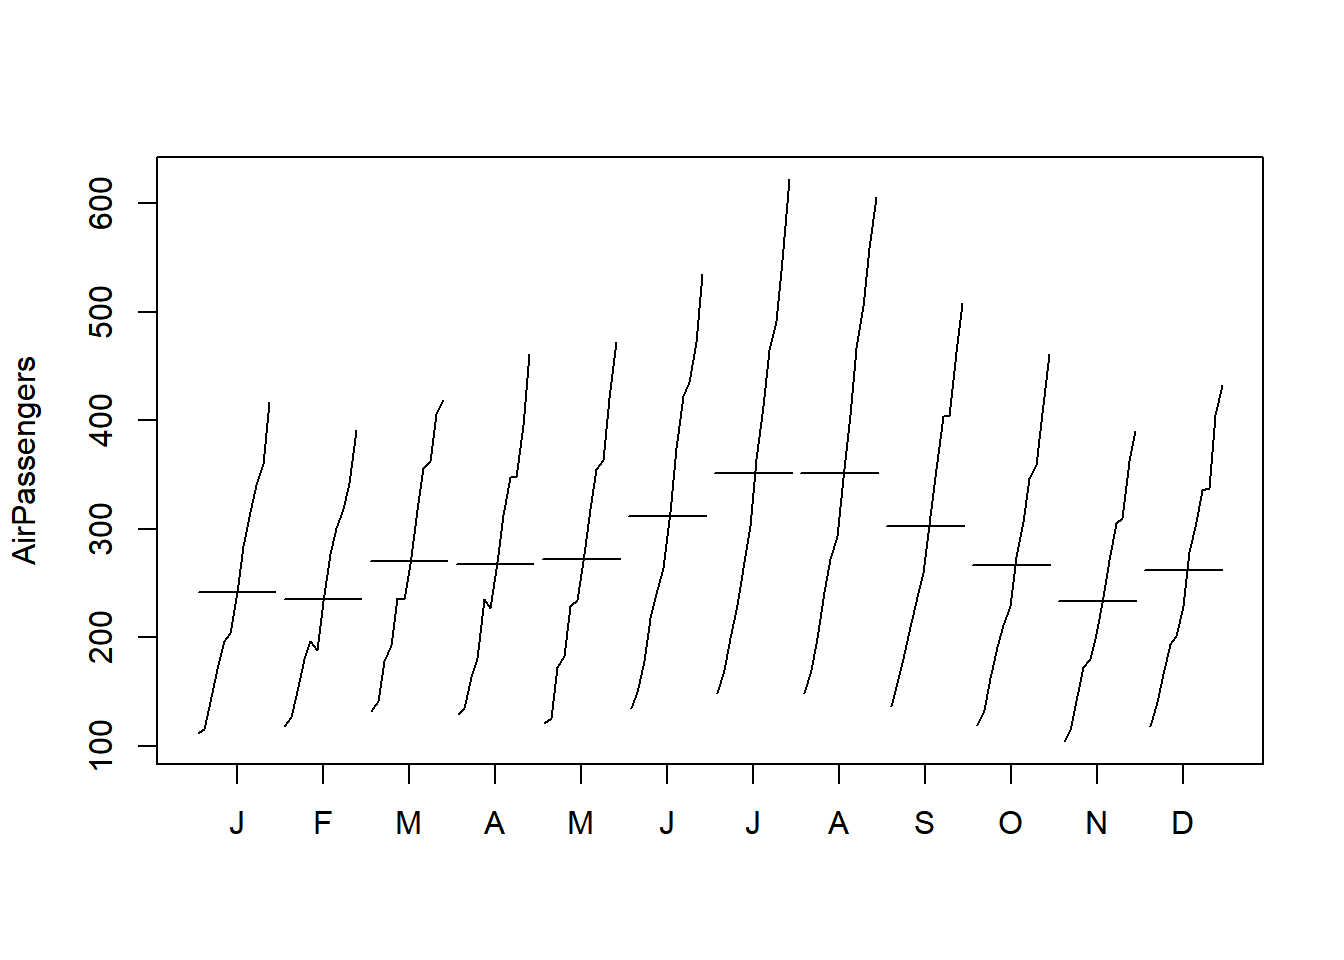
\includegraphics{sazonalidade_files/figure-pdf/fig-AirPassengersMonthplot-2.pdf}

}

\caption{\label{fig-AirPassengersMonthplot-2}Gráfico de subséries da
série AirPassengers. Observe as tendências monótona crescente em cada
subgráfico}

}

\end{minipage}%

\end{figure}

Abaixo, vamos estimar a tendência da série e removê-la. Note que o
padrão das subséries se altera, mostrando o real comportamento do padrão
sazonal: é uma tendência de crescimento nos meses de verão americano
(junho, julho e agosto) e um padrão de queda começando em novembro e
pegando so três subsequentes meses do inverno.

\begin{Shaded}
\begin{Highlighting}[]
\CommentTok{\# estimação da tendência via loess}
\NormalTok{tempo }\OtherTok{\textless{}{-}} \DecValTok{1} \SpecialCharTok{:} \FunctionTok{length}\NormalTok{(AirPassengers)}
\NormalTok{model }\OtherTok{\textless{}{-}} \FunctionTok{loess}\NormalTok{( AirPassengers }\SpecialCharTok{\textasciitilde{}}\NormalTok{tempo)}
\NormalTok{tend }\OtherTok{\textless{}{-}} \FunctionTok{fitted}\NormalTok{(model)}

\CommentTok{\# série sem tendência e o gráfico de subséries}
\FunctionTok{plot}\NormalTok{( AirPassengers}\SpecialCharTok{{-}}\NormalTok{tend)}
\end{Highlighting}
\end{Shaded}

\begin{figure}[H]

{\centering \includegraphics{sazonalidade_files/figure-pdf/unnamed-chunk-6-1.pdf}

}

\end{figure}

\begin{Shaded}
\begin{Highlighting}[]
\FunctionTok{monthplot}\NormalTok{(AirPassengers}\SpecialCharTok{{-}}\NormalTok{tend)}
\end{Highlighting}
\end{Shaded}

\begin{figure}[H]

{\centering 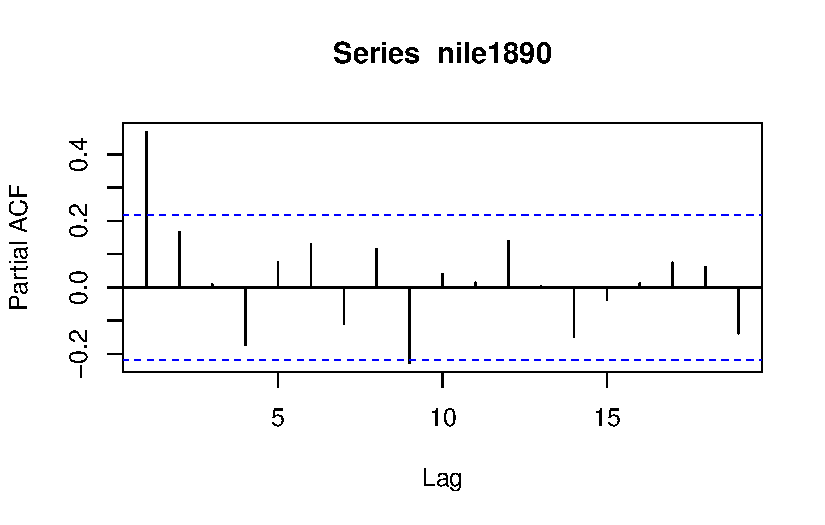
\includegraphics{sazonalidade_files/figure-pdf/unnamed-chunk-6-2.pdf}

}

\end{figure}

\(\blacksquare\)

\end{example}

\hypertarget{dessazonalizauxe7uxe3o}{%
\section{Dessazonalização}\label{dessazonalizauxe7uxe3o}}

Existem séries que apresentam tanto tendência quanto sazonalidade. Isso
pode dificultar o estudo da tendência, uma vez que a sazonalidade
interfere no movimento de subida e descida da série. Nesses casos, é
interessante obter uma estimativa da parte sazonal para removê-la da
série.

Considere a série \[y_t = T^\star(t)+s^\star(t)+\varepsilon_t,\] onde
\(T^\star(t)\) é a tendência e \(s^\star(t)\) uma função periódica, com
período igual a \(p\). É sempre verdade que existe uma constante real
\(c\) tal que \[\sum_{j=1}^p s^\star(t+j)=c\] para qualquer
\(t=0,1,\ldots\). Contudo, note que \(c\) é uma constante (que, por sua
vez, faz parte da tendência da série). Fazendo \(T(t)=T^\star(t)+c\) e
\(s(t)=s^\star(t)-c\), teremos
\[y_t = T^\star(t)+c + s^\star(t)-c+\varepsilon_t=T(t)+ s(t)+\varepsilon_t,\]

e sempre podemos assumir que \[\sum_{t=1}^{p}s(t)=0.\] Isto é
equivalente a afirmar que o efeito sazonal desaparece quando as \(p\)
observações são agregadas. Deste modo, o estimador para tendência
\(p\)-MM estima a tendência sem o efeito sazonal.

Considere novamente a série com o número de óbitos por doenças
pulmonares no Reino Unido. A figura abaixo mostra a série original e a
tendência, estimada pela 12-MM. Observe o padrão claro de tendência
decrescente.

\begin{figure}

\end{figure}

\hypertarget{decomposiuxe7uxf5es-de-suxe9ries}{%
\section{Decomposições de
séries}\label{decomposiuxe7uxf5es-de-suxe9ries}}

Em geral, assume-se que a série temporal admite a seguinte decomposição:
\[x_t=T(t)+s(t)+\varepsilon_t\]

A estimação não paramétrica dos componentes da decomposição constitui-se
de ferramenta exploratória essencial para a análise de séries temporais.
A decomposição clássica é realizada através dos seguintes passos:

\begin{itemize}
\item
  Estime a tendência dessazoanlizada, utilizando a \(p\)-MM, obtendo
  \(\hat{T}\)
\item
  Remova a tendência da série: \(\tilde{x}_t=x_t-\hat{T}\)
\item
  Encontre as \(p\) subséries de \(\tilde{x}\) e estime os valores de
  \(s\) através de suas médias.
\item
  Estime os resíduos: \(\hat{\varepsilon}_t=x_t-\hat{T}(t)-\hat{s}(t)\)
  A Figure~\ref{fig-ldeathsDecomposicaoClassica} apresenta a
  decomposição clássica da série de óbitos pode doenças pulmonares no
  Reino Unido.
\end{itemize}

\begin{Shaded}
\begin{Highlighting}[]
\FunctionTok{plot}\NormalTok{(}\FunctionTok{decompose}\NormalTok{(ldeaths))}
\end{Highlighting}
\end{Shaded}

\begin{figure}

\begin{minipage}[t]{\linewidth}

{\centering 

\raisebox{-\height}{

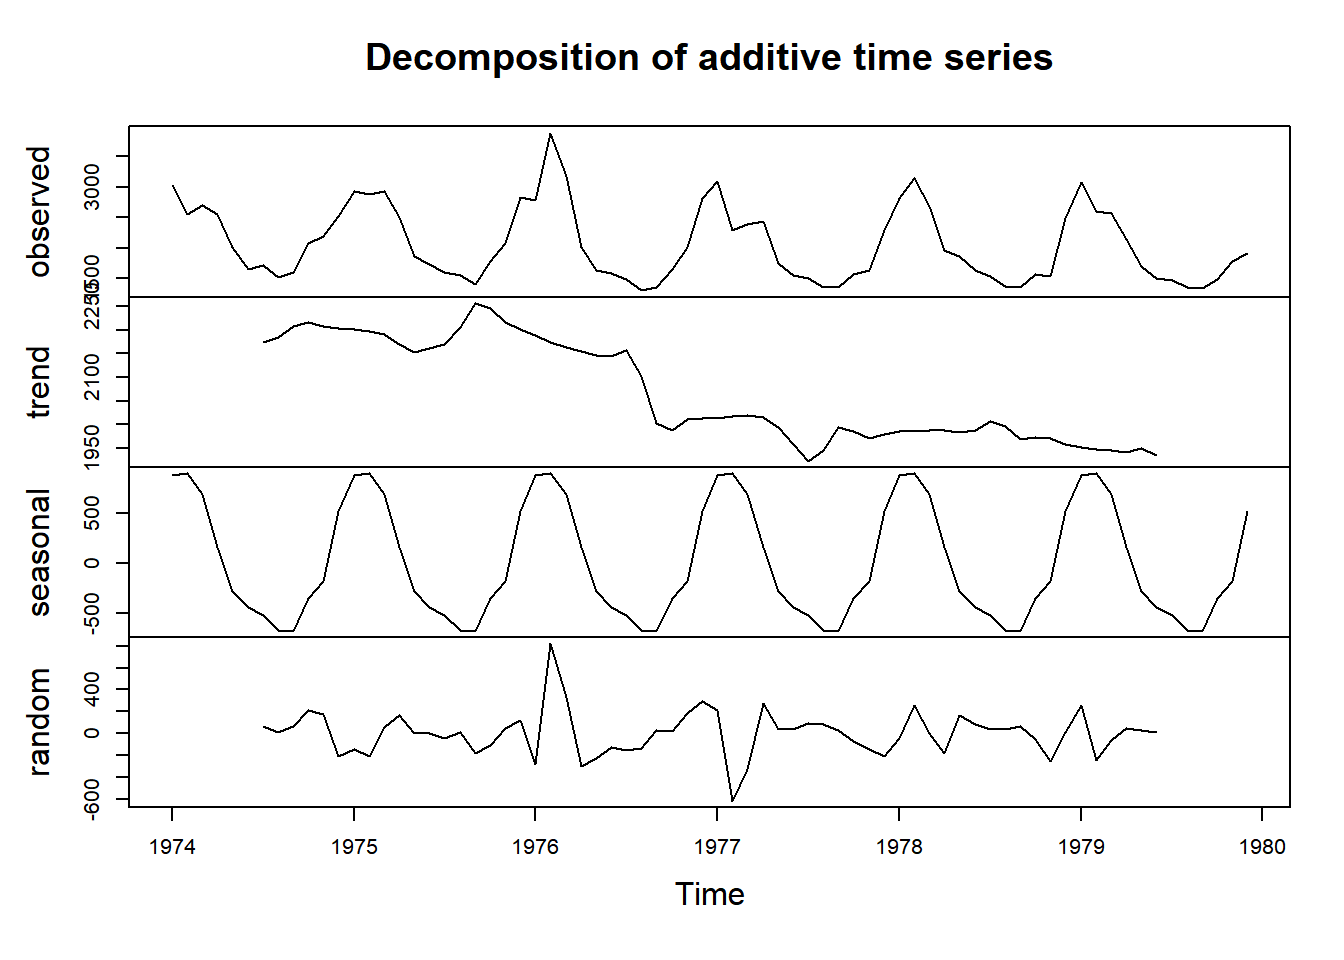
\includegraphics{sazonalidade_files/figure-pdf/fig-ldeathsDecomposicaoClassica-1.pdf}

}

\caption{\label{fig-ldeathsDecomposicaoClassica}Decomposição da série de
óbitos por doenças pulmonares no Reino Unido}

}

\end{minipage}%

\end{figure}

Como é utilizada uma média móvel, a estimativa da tendência e do ruído é
prejudicada no início e fim da série. Outro problema que este método não
consegue estimar padrões sazonais que não sejam representamos por uma
função periódica. Para ilustrar, apresentamos abaixo a decomposição
clássica da série \texttt{AirPassengers}. Como a estimação da parte
sazonal utilizou a média das subséries, as tendências sazonais vistas no
Example~\ref{exm-AirPassengersMonthplot} foram para os resíduos
(identificados co)

\begin{Shaded}
\begin{Highlighting}[]
\FunctionTok{plot}\NormalTok{(}\FunctionTok{decompose}\NormalTok{(AirPassengers))}
\end{Highlighting}
\end{Shaded}

\begin{figure}[H]

{\centering 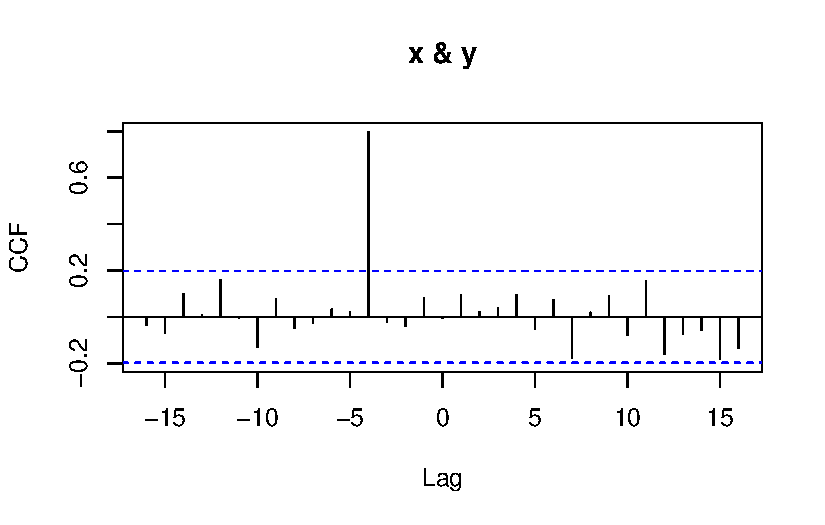
\includegraphics{sazonalidade_files/figure-pdf/unnamed-chunk-9-1.pdf}

}

\end{figure}

Uma solução mais robusta é conhecida como STL, que realiza uma séries de
estimativas de tendência, tanto para a geral quanto para a sazonal,
utilizando o loess. Os detalhes podem ser vistos no paper original
\href{https://www.scb.se/contentassets/ca21efb41fee47d293bbee5bf7be7fb3/stl-a-seasonal-trend-decomposition-procedure-based-on-loess.pdf}{STL}
Abaixo, apresentamos o STL para a série \texttt{AirPassengers}. Observe
que a sazonalidade foi melhor estimada, embora ainda exista um padrão
sazonal nos resíduos.

\begin{Shaded}
\begin{Highlighting}[]
\CommentTok{\# além da série, devemos colocar o período desejado na função }
\FunctionTok{plot}\NormalTok{(}\FunctionTok{stl}\NormalTok{(AirPassengers, }\DecValTok{12}\NormalTok{))}
\end{Highlighting}
\end{Shaded}

\begin{figure}[H]

{\centering 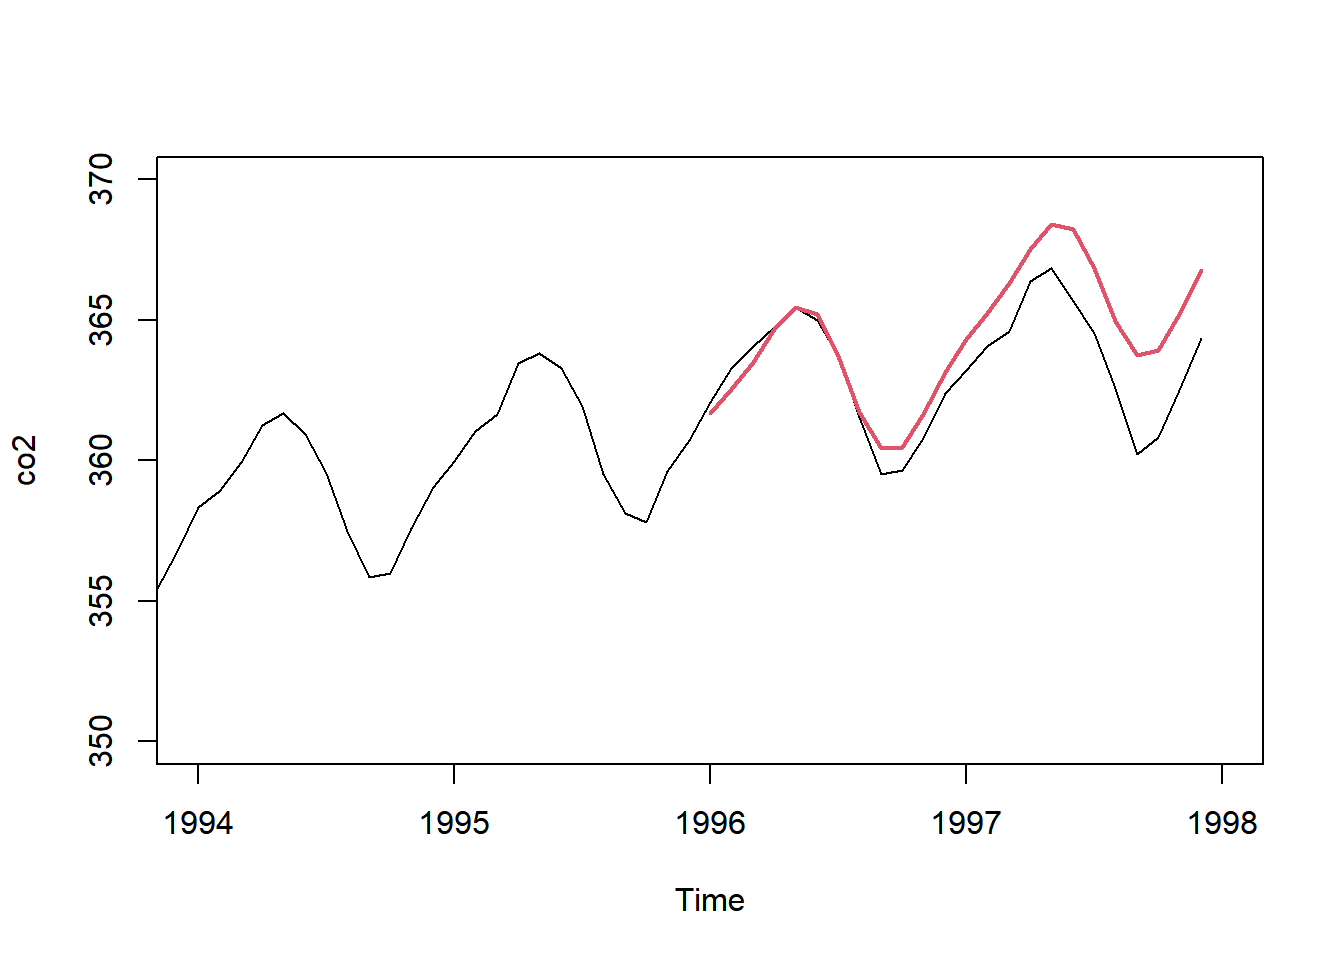
\includegraphics{sazonalidade_files/figure-pdf/unnamed-chunk-10-1.pdf}

}

\end{figure}

\hypertarget{modelo-de-forma-livre---ou-fatores-sazonais}{%
\section{Modelo de Forma livre - ou fatores
sazonais}\label{modelo-de-forma-livre---ou-fatores-sazonais}}

Considere uma série temporal com sazonalidade dada por uma função
periódica \(s(.)\) de período \(p\). Sejam \[\beta_j=s(t+jp).\] Os
parâmetros \(\beta_1,\ldots,\beta_p\) são denominados fatores sazonais.
Note que é necessário colocar a restrição
\[\beta_p = -\beta_1-\cdots -\beta_{p-1},\] pois
\[\sum_{j=1}^p\beta_j=0\] (ou seja, existem na prática \(p-1\) fatores
sazonais para serem estimados).

\begin{example}[]\protect\hypertarget{exm-fatorSazonalIlustracao}{}\label{exm-fatorSazonalIlustracao}

Seja \(x_t\) uma série sazonal de período \(p=4\) (por, exemplo, em
dados trimestrais). Então \[\begin{align*}
        E(x_t)&=s(t)=\beta_1, t=1,5,9 ,\ldots,\\
        E(x_t)&=s(t)=\beta_2, t=2,6,10,\ldots,\\
        E(x_t)&=s(t)=\beta_3, t=3,7,11,\ldots,\\
        E(x_t)&=s(t)=-\beta_1-\beta_2-\beta_3, t=4,8,12,\ldots,\\
        \end{align*}\]

\end{example}

Seja \(\boldsymbol{E}_{j,m-1}\) o vetor coluna de comprimento \(m-1\)
que possui a \(j\)-ésima entrada igual a 1 e as demais iguais a zero.
Por exemplo \[\boldsymbol{E}_{2,3}=\left(\begin{array}{c}0 \\ 1 \\ 0
\end{array}\right).\] Para um período \(p\) e para \(j=1,\ldots,p-1\)
faça \[\begin{align}
        \boldsymbol{f}_{j+kp} = \boldsymbol{E}_{j,p-1}
        \end{align}\] com \(k=0,1,2,\ldots\). Para \(s=1,2,\ldots\)
\[\begin{equation}
        \boldsymbol{f}_{sp} = -\textbf{1}_{p-1}
        \end{equation}\]

Então, \[x_t=\boldsymbol{f}_t' \boldsymbol{\beta}+\varepsilon_t,\] onde
\(\boldsymbol{\beta}'=(\beta_1,\ldots,\beta_{p-1})\) representa os
efeitos sazonais. Disto, teremos
\[\boldsymbol{x}=\boldsymbol{F}_n'\boldsymbol{\beta}+\boldsymbol{\varepsilon}\]
onde a matriz \(\boldsymbol{F}_n\) é formada pelas colunas
\(\boldsymbol{f}_1,\ldots,\boldsymbol{f}_p\).

Portanto, a estimação de \(\beta\) é feita através da teoria de modelos
lineares.

\begin{example}[]\protect\hypertarget{exm-nottemFatores}{}\label{exm-nottemFatores}

Considere novamente a série \texttt{nottem}, representada na figura
abaixo.

\begin{Shaded}
\begin{Highlighting}[]
\FunctionTok{ts.plot}\NormalTok{(nottem)}
\FunctionTok{abline}\NormalTok{(}\AttributeTok{h =} \FunctionTok{mean}\NormalTok{(nottem))}
\end{Highlighting}
\end{Shaded}

\begin{figure}[H]

{\centering 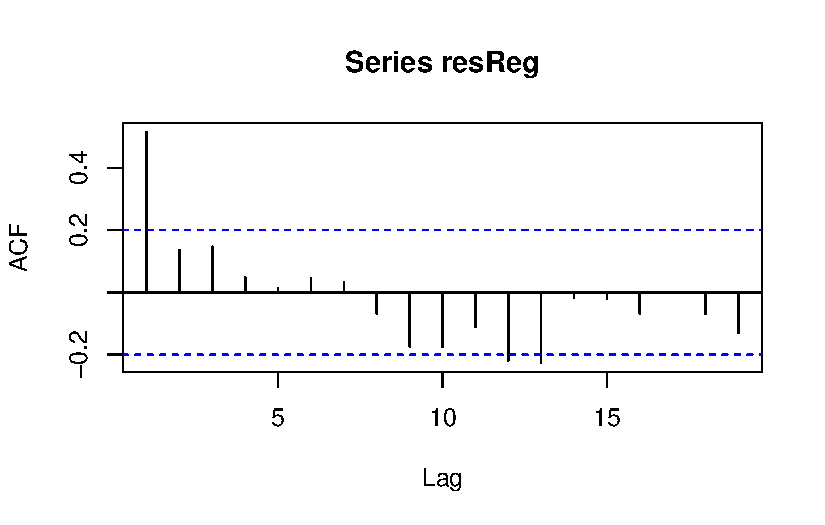
\includegraphics{sazonalidade_files/figure-pdf/unnamed-chunk-11-1.pdf}

}

\end{figure}

Observe que a série pode ser vista como uma função periódica com um
nível constante (conhecido em regressão como intecepto):

\[x_t = \mu+s(t)+\varepsilon_t\]

Considerando que os erros são ergódicos, podemos estimar a média \(\mu\)
pela média amostral. Deste modo, a série sem tendência é:
\[\tilde{x}_t=x_t-\bar{x}=s(t)+\varepsilon_t\] Vamos ajustar um modelo
linear para \(\tilde{x}\). Para construir a matriz de regressão
\(\boldsymbol{F}'_n\) vamos utiliza a função \texttt{cycle} que
identifica o índice do padrão sazonal associado a cada observação.

\begin{Shaded}
\begin{Highlighting}[]
\NormalTok{xtil }\OtherTok{\textless{}{-}}\NormalTok{ nottem }\SpecialCharTok{{-}} \FunctionTok{mean}\NormalTok{(nottem) }
\NormalTok{mes }\OtherTok{\textless{}{-}} \FunctionTok{cycle}\NormalTok{(nottem)}
\NormalTok{mes }\OtherTok{\textless{}{-}} \FunctionTok{as.factor}\NormalTok{(mes)}
\NormalTok{mod }\OtherTok{\textless{}{-}} \FunctionTok{lm}\NormalTok{( xtil }\SpecialCharTok{\textasciitilde{}}\NormalTok{ mes }\SpecialCharTok{{-}} \DecValTok{1}\NormalTok{)}
\NormalTok{mod}
\end{Highlighting}
\end{Shaded}

\begin{verbatim}

Call:
lm(formula = xtil ~ mes - 1)

Coefficients:
   mes1     mes2     mes3     mes4     mes5     mes6     mes7     mes8  
-9.3446  -9.8496  -6.8446  -2.7496   3.5204   9.0004  12.8604  11.4804  
   mes9    mes10    mes11    mes12  
 7.4404   0.4554  -6.4596  -9.5096  
\end{verbatim}

Nos resultados acima podemos notar que os meses de Novembro até Abril
possuem temperaturas menores que a média. O gráfico dos efeitos sazonais
é dado a seguir, mostrando que a passagem dos meses possui um padrão de
onda, como um cosseno.

\begin{Shaded}
\begin{Highlighting}[]
\FunctionTok{plot.new}\NormalTok{()}
\FunctionTok{plot.window}\NormalTok{(}\AttributeTok{xlim =} \FunctionTok{c}\NormalTok{(}\DecValTok{0}\NormalTok{,}\DecValTok{13}\NormalTok{), }\AttributeTok{ylim=} \FunctionTok{c}\NormalTok{(}\SpecialCharTok{{-}}\DecValTok{11}\NormalTok{,}\DecValTok{11}\NormalTok{))}
\FunctionTok{points}\NormalTok{(}\FunctionTok{coefficients}\NormalTok{(mod), }\AttributeTok{pch =} \DecValTok{16}\NormalTok{)}
\FunctionTok{axis}\NormalTok{(}\DecValTok{1}\NormalTok{, }\AttributeTok{at =} \DecValTok{1}\SpecialCharTok{:}\DecValTok{12}\NormalTok{, }\AttributeTok{labels =} \FunctionTok{c}\NormalTok{(}\StringTok{\textquotesingle{}J\textquotesingle{}}\NormalTok{,}\StringTok{\textquotesingle{}F\textquotesingle{}}\NormalTok{,}\StringTok{\textquotesingle{}M\textquotesingle{}}\NormalTok{,}\StringTok{\textquotesingle{}A\textquotesingle{}}\NormalTok{,}\StringTok{\textquotesingle{}M\textquotesingle{}}\NormalTok{,}\StringTok{\textquotesingle{}J\textquotesingle{}}\NormalTok{,}\StringTok{\textquotesingle{}J\textquotesingle{}}\NormalTok{,}\StringTok{\textquotesingle{}A\textquotesingle{}}\NormalTok{,}\StringTok{\textquotesingle{}S\textquotesingle{}}\NormalTok{,}\StringTok{\textquotesingle{}O\textquotesingle{}}\NormalTok{,}\StringTok{\textquotesingle{}N\textquotesingle{}}\NormalTok{,}\StringTok{\textquotesingle{}D\textquotesingle{}}\NormalTok{))}
\FunctionTok{axis}\NormalTok{(}\DecValTok{2}\NormalTok{)}
\FunctionTok{title}\NormalTok{(}\AttributeTok{ylab =} \StringTok{\textquotesingle{}Valor do fator sazonal\textquotesingle{}}\NormalTok{,}\AttributeTok{xlab=}\StringTok{\textquotesingle{}Fator sazonal\textquotesingle{}}\NormalTok{)}
\end{Highlighting}
\end{Shaded}

\begin{figure}[H]

{\centering 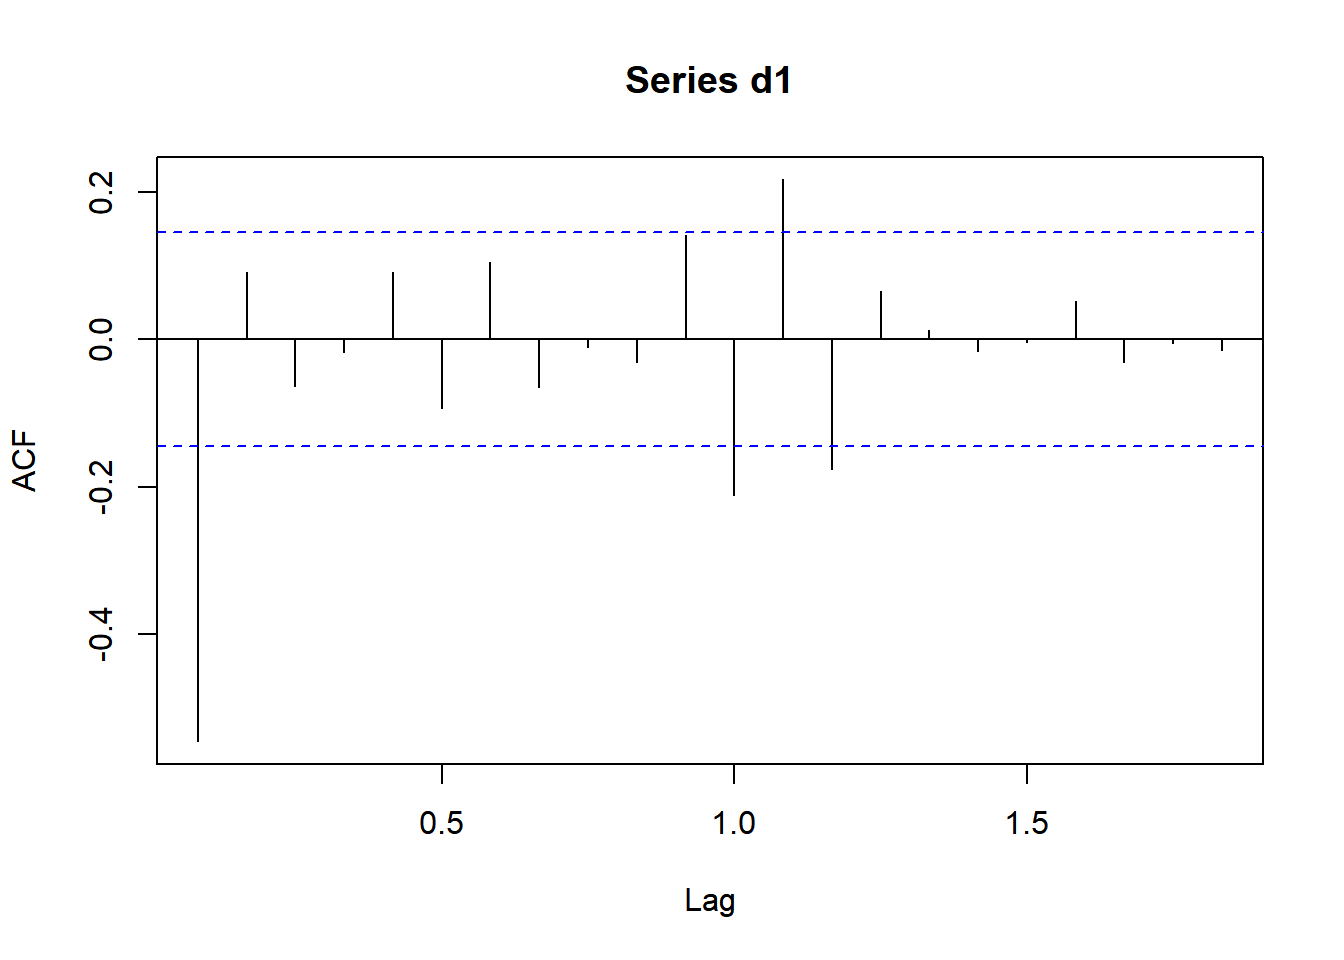
\includegraphics{sazonalidade_files/figure-pdf/unnamed-chunk-13-1.pdf}

}

\end{figure}

Abaixo analisamos os resíduos do modelo. Os resíduos parecem flutuar e
torno de zero com variância constante. O correlograma apresenta algumas
leves autocorrelações nas defasagens 1 e 2. O teste de Shapiro-Wilks não
rejeita a normalidade, mas o teste de Box-Pierce rejeita a hipótese de
ruído branco. Voltaremos a este problema posteriormente.

\begin{Shaded}
\begin{Highlighting}[]
\NormalTok{res }\OtherTok{\textless{}{-}} \FunctionTok{residuals}\NormalTok{(mod)}
\FunctionTok{ts.plot}\NormalTok{(res)}
\FunctionTok{acf}\NormalTok{(res)}
\end{Highlighting}
\end{Shaded}

\begin{figure}

\begin{minipage}[t]{0.50\linewidth}

{\centering 

\raisebox{-\height}{

\includegraphics{sazonalidade_files/figure-pdf/unnamed-chunk-14-1.pdf}

}

\caption{Gráfico dos ressíduos}

}

\end{minipage}%
%
\begin{minipage}[t]{0.50\linewidth}

{\centering 

\raisebox{-\height}{

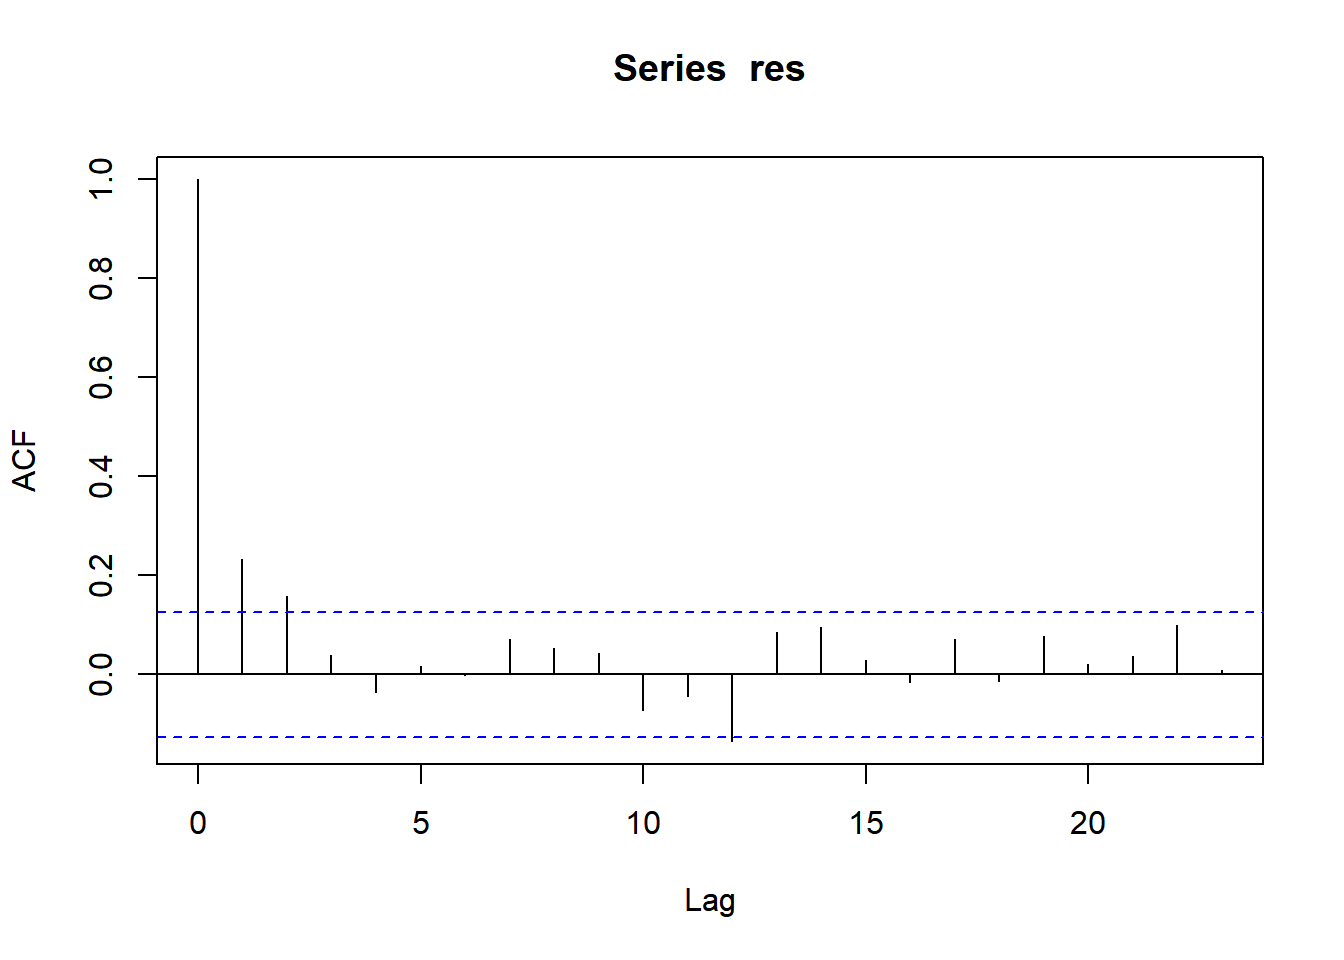
\includegraphics{sazonalidade_files/figure-pdf/unnamed-chunk-14-2.pdf}

}

\caption{Correlograma dos resíduos}

}

\end{minipage}%

\end{figure}

\begin{Shaded}
\begin{Highlighting}[]
\FunctionTok{shapiro.test}\NormalTok{(res)}
\end{Highlighting}
\end{Shaded}

\begin{verbatim}

    Shapiro-Wilk normality test

data:  res
W = 0.99125, p-value = 0.1612
\end{verbatim}

\begin{Shaded}
\begin{Highlighting}[]
\FunctionTok{Box.test}\NormalTok{(res)}
\end{Highlighting}
\end{Shaded}

\begin{verbatim}

    Box-Pierce test

data:  res
X-squared = 13.109, df = 1, p-value = 0.0002939
\end{verbatim}

\(\blacksquare\)

\end{example}

\hypertarget{regressuxe3o-harmuxf4nica-simples}{%
\section{Regressão harmônica
simples}\label{regressuxe3o-harmuxf4nica-simples}}

\hypertarget{a-funuxe7uxe3o-harmuxf4nica}{%
\subsection{A função harmônica}\label{a-funuxe7uxe3o-harmuxf4nica}}

A função \[\begin{equation}
    s(t) = A \cos\left( 2\pi \omega t_i +\phi \right),
\end{equation}\] é denominada harmônico, onde \(A\) e
\(\phi\in(0,2\pi)\) são denominados amplitude e fase. Essa função é
periódica, com período igual a \(p = 1/\omega\) onde \(\omega\) é
denominado frequência (angular).

\begin{Shaded}
\begin{Highlighting}[]
\FunctionTok{curve}\NormalTok{( }\FunctionTok{cos}\NormalTok{( }\DecValTok{2}\SpecialCharTok{*}\NormalTok{pi}\SpecialCharTok{/}\DecValTok{12} \SpecialCharTok{*}\NormalTok{x), }\DecValTok{0}\NormalTok{,}\DecValTok{24}\NormalTok{, }\AttributeTok{lwd =} \DecValTok{2}\NormalTok{, }\AttributeTok{ylab =} \StringTok{\textquotesingle{}\textquotesingle{}}\NormalTok{)}
\FunctionTok{curve}\NormalTok{( .}\DecValTok{5}\SpecialCharTok{*}\FunctionTok{cos}\NormalTok{( }\DecValTok{2}\SpecialCharTok{*}\NormalTok{pi}\SpecialCharTok{/}\DecValTok{12} \SpecialCharTok{*}\NormalTok{x), }\AttributeTok{add =}\NormalTok{ T, }\AttributeTok{lty =} \DecValTok{2}\NormalTok{,}\AttributeTok{lwd =} \DecValTok{2}\NormalTok{)}
\FunctionTok{curve}\NormalTok{( }\FunctionTok{cos}\NormalTok{( }\DecValTok{2}\SpecialCharTok{*}\NormalTok{pi}\SpecialCharTok{/}\DecValTok{12} \SpecialCharTok{*}\NormalTok{x}\SpecialCharTok{+}\DecValTok{2}\NormalTok{), }\DecValTok{0}\NormalTok{,}\DecValTok{24}\NormalTok{, }\AttributeTok{lwd =} \DecValTok{2}\NormalTok{, }\AttributeTok{ylab =} \StringTok{\textquotesingle{}\textquotesingle{}}\NormalTok{)}
\FunctionTok{curve}\NormalTok{( }\FunctionTok{cos}\NormalTok{( }\DecValTok{2}\SpecialCharTok{*}\NormalTok{pi}\SpecialCharTok{/}\DecValTok{12} \SpecialCharTok{*}\NormalTok{x }\SpecialCharTok{+} \DecValTok{4}\NormalTok{), }\AttributeTok{add =}\NormalTok{ T, }\AttributeTok{lty =} \DecValTok{2}\NormalTok{,}\AttributeTok{lwd =} \DecValTok{2}\NormalTok{)}
\FunctionTok{curve}\NormalTok{( }\FunctionTok{cos}\NormalTok{( }\DecValTok{2}\SpecialCharTok{*}\NormalTok{pi}\SpecialCharTok{/}\DecValTok{12} \SpecialCharTok{*}\NormalTok{x), }\DecValTok{0}\NormalTok{,}\DecValTok{24}\NormalTok{, }\AttributeTok{lwd =} \DecValTok{2}\NormalTok{, }\AttributeTok{ylab =} \StringTok{\textquotesingle{}\textquotesingle{}}\NormalTok{)}
\FunctionTok{curve}\NormalTok{( }\FunctionTok{cos}\NormalTok{( }\DecValTok{2}\SpecialCharTok{*}\NormalTok{pi}\SpecialCharTok{/}\DecValTok{6} \SpecialCharTok{*}\NormalTok{x), }\AttributeTok{add =}\NormalTok{ T, }\AttributeTok{lty =} \DecValTok{2}\NormalTok{,}\AttributeTok{lwd =} \DecValTok{2}\NormalTok{)}
\end{Highlighting}
\end{Shaded}

\begin{figure}

\begin{minipage}[t]{0.50\linewidth}

{\centering 

\raisebox{-\height}{

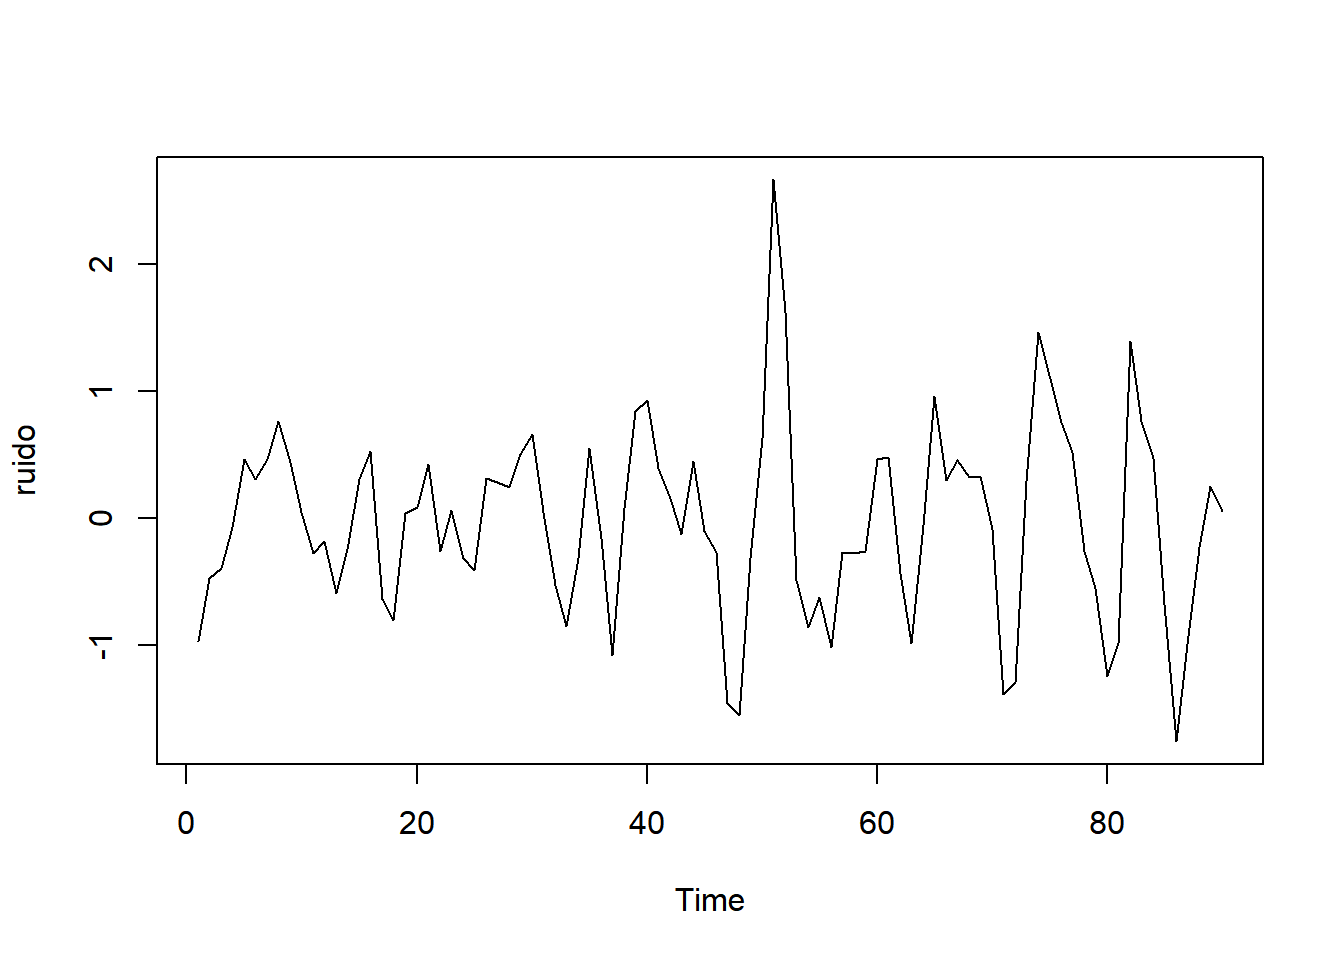
\includegraphics{sazonalidade_files/figure-pdf/unnamed-chunk-16-1.pdf}

}

\caption{A amplitude representa o valor máximo e mínimo do harmônico. No
gráfico estão representados harmônicos de período 12 com diferentes
amplitudes. Linha cheia: A=1. Linha tracejada: A=0,5}

}

\end{minipage}%
%
\begin{minipage}[t]{0.50\linewidth}

{\centering 

\raisebox{-\height}{

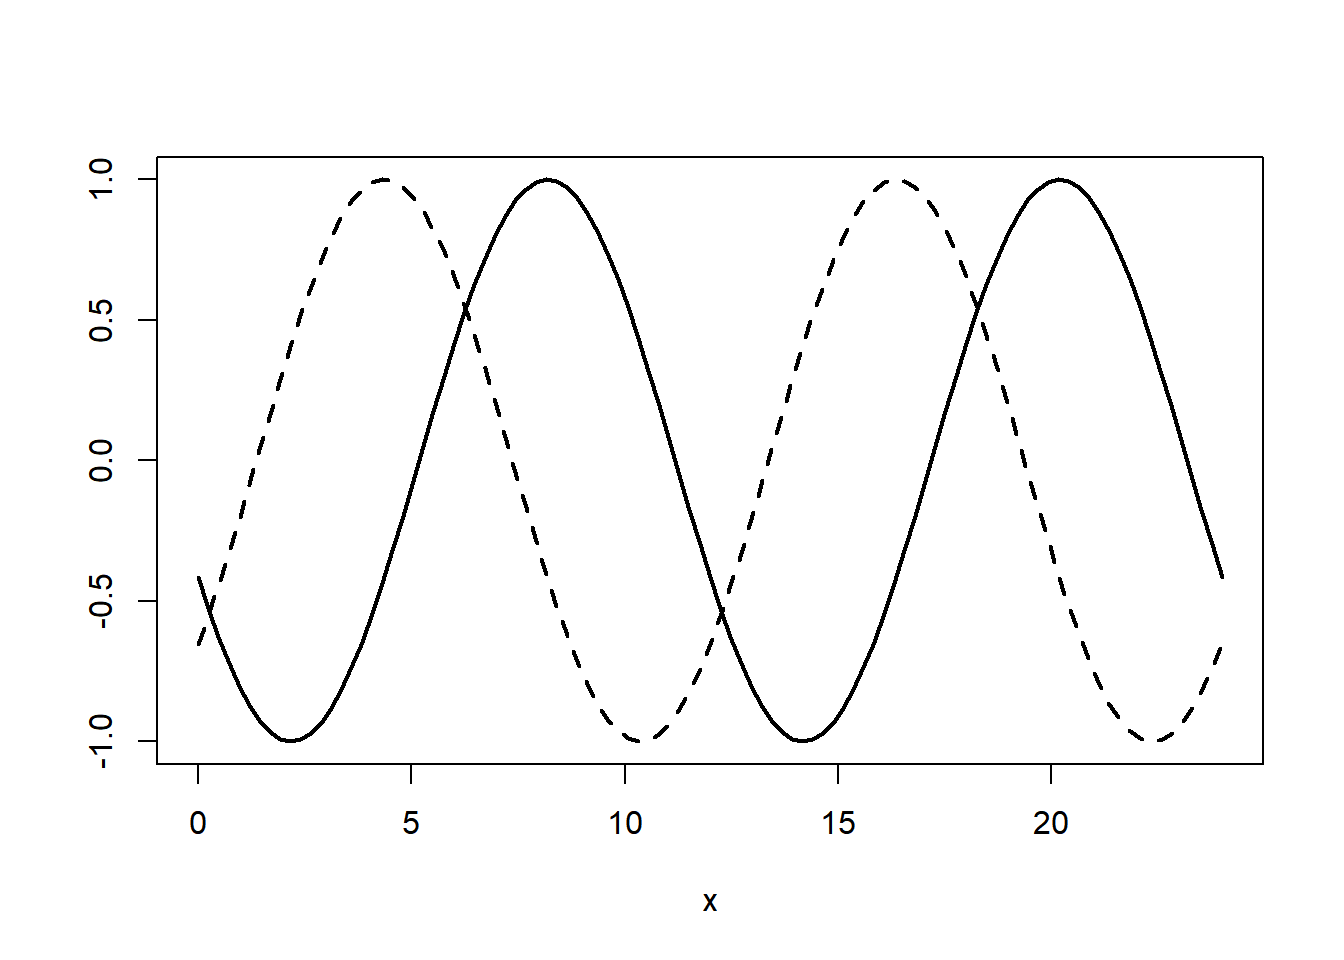
\includegraphics{sazonalidade_files/figure-pdf/unnamed-chunk-16-2.pdf}

}

\caption{A fase tem papel de locação, deslocando da onda mas mantendo
sua forma. No gráfico estão representados harmônicos de período 12 com
diferentes fases. Linha cheia: \(\phi=2\). Linha tracejada: \(\phi=4\)}

}

\end{minipage}%
\newline
\begin{minipage}[t]{0.50\linewidth}

{\centering 

\raisebox{-\height}{

\includegraphics{sazonalidade_files/figure-pdf/unnamed-chunk-16-3.pdf}

}

\caption{A frequência representa o número de voltas por unidade de
tempo. No gráfico estão representados harmônicos com frequências
diferentes. Linha cheia: \(\omega=1/12\) (padrão anual). Linha
tracejada: \(\omega=1/6\) (padrão semestral)}

}

\end{minipage}%

\end{figure}

\textbf{Cuidado.} Período é o tempo necessário para que o padrão sazonal
se repita, dando uma volta completa. Já a frequência é o número de vezes
que o padrão se repete por unidade de tempo. Por exemplo, para \(p=12\)
(meses), \(\omega=1/12\) implica que cada unidade do tempo (mês)
representa um doze ávos de uma volta.

Entretanto, quando criamos um objeto do tipo \texttt{ts} alimentamos o
argumento \texttt{frequency} com o valor do período. A aparente confusão
ocorre porque o argumento \texttt{frequency} se refere ao número de
observações (ou seja, frequência) por unidade de tempo.

Também é possível escrever um objeto \texttt{ts} atribuíndo o valor
\(\omega\) através do argumento \texttt{deltat}. Por exemplo, para um
período de 12 meses, usamos \texttt{deltat=1/12}.

Pela definição, como \(\omega=1/p\), teremos que \(\omega\in(0,1)\).
Assuma que \(a=\omega+1/2\), onde \(\omega\in(0,1/2)\). Então, podemos
notar que
\[\begin{align}A\cos(2\pi\omega t + \phi ) &= A\cos\left( 2\pi\left(a-\frac{1}{2}\right) t + \phi \right)\\
&=A\cos(2\pi at+\phi)\cos\left(\pi t\right)\\
&=A^\star\cos(2\pi a t + \phi).\end{align}\] onde
\(A^\star=A\cos(\pi t)\). Na prática, é impossível distinguir entre
\((A,\omega)\) e \((A^\star, a)\). Para permitir a existência da
identificabilidade, vamos assumir que \(A>0\) e \(\omega\in(0,1/2)\).
Isto implica que o menor período detectátvel é \(p = 2\).

\hypertarget{o-modelo-de-regressuxe3o-harmuxf4nica-simples}{%
\subsection{O modelo de regressão harmônica
simples}\label{o-modelo-de-regressuxe3o-harmuxf4nica-simples}}

O modelo de regressão harmônica simples é dado por
\[y_t = A \cos\left( 2\pi\omega t_i +\phi \right) + \varepsilon_t,\]
onde \(\varepsilon_t\) é um ruído branco. Como \(\omega\) é considerado
conhecido, este modelo pode ser linearizado:
\[A\cos\left(2\pi\omega t_i + \phi \right)=A\left[ \cos(2\pi\omega t_i)\cos(\phi) - \sin(2\pi\omega t_i)\sin(\phi)\right]\]
e, fazendo \(\beta_1=A\cos(\phi)}\) e \(\beta_2 =-A\sin(\phi)\), teremos
que
\[y_t=\beta_1\cos(2\pi\omega t_i)+\beta_2\sin(2\pi\omega)+\varepsilon_t\]
Note que sempre é possível recuperar os parâmetros originais:
\[\begin{align*}
    \left\{
    \begin{array}{l}
    \beta_1 = A\cos(\phi) \\
    \beta_2 = -A\sin(\phi) \\
    \end{array}\right.  \Rightarrow     
    \left\{
    \begin{array}{l}
    \beta_1^2 = A^2\cos(\phi)^2 \\
    \beta_2^2 = A^2\sin(\phi)^2 \\
    \end{array}\right.  \Rightarrow                 
    \left\{
    \begin{array}{l}
    A = \sqrt{\beta_1^2 + \beta_2^2}\\
    \phi = \cos^{-1}\left(\frac{\beta_1}{A}\right) \\
    \end{array}\right.
    \end{align*}\]

Fazendo \[\begin{align}
        \boldsymbol{\beta}' &= (\beta_1, \beta_2) \\
        \boldsymbol{f}_t' &= (\cos(\omega t_i), \sin(\omega t_i))
        \end{align}\] teremos
\[\boldsymbol{f}_t'\boldsymbol{\beta}=A\cos(\omega t_i + \phi).\]
Portanto, podemos escrever: \[\begin{equation}
        y_t = \boldsymbol{f}_t'\boldsymbol{\beta}+\varepsilon_t
        \end{equation}\] Considerando
\(\varepsilon_t\sim\hbox{Normal}(0,\nu)\) teremos
\[\boldsymbol{y}|\boldsymbol{\beta},\nu\sim\hbox{Normal}( \boldsymbol{F}_n'\boldsymbol{\beta},\nu\textbf{I}_T).\]

\begin{example}[]\protect\hypertarget{exm-nottemHarmonico1}{}\label{exm-nottemHarmonico1}

Considere novamente a série \texttt{nottem}. A função \texttt{harmonic}
do pacote \texttt{TSA} constrói a matriz necessária para compor o modelo
de regressão harmônica simples.

\begin{Shaded}
\begin{Highlighting}[]
\FunctionTok{require}\NormalTok{(TSA)}
\end{Highlighting}
\end{Shaded}

\begin{verbatim}
Carregando pacotes exigidos: TSA
\end{verbatim}

\begin{verbatim}
Warning: package 'TSA' was built under R version 4.3.2
\end{verbatim}

\begin{verbatim}

Attaching package: 'TSA'
\end{verbatim}

\begin{verbatim}
The following objects are masked from 'package:stats':

    acf, arima
\end{verbatim}

\begin{verbatim}
The following object is masked from 'package:utils':

    tar
\end{verbatim}

\begin{Shaded}
\begin{Highlighting}[]
\NormalTok{har }\OtherTok{\textless{}{-}} \FunctionTok{harmonic}\NormalTok{(nottem)}
\NormalTok{mod }\OtherTok{\textless{}{-}} \FunctionTok{lm}\NormalTok{( nottem }\SpecialCharTok{\textasciitilde{}}\NormalTok{ har)}
\NormalTok{mod}
\end{Highlighting}
\end{Shaded}

\begin{verbatim}

Call:
lm(formula = nottem ~ har)

Coefficients:
   (Intercept)  harcos(2*pi*t)  harsin(2*pi*t)  
        49.040         -11.473          -1.391  
\end{verbatim}

Note que não removemos a média da série, logo a mesma está sendo
estimada pelo intercepto \(\mu\). O gráfico do harmônico gerado é
mostrado abaixo.

\begin{Shaded}
\begin{Highlighting}[]
\NormalTok{param }\OtherTok{\textless{}{-}} \FunctionTok{coefficients}\NormalTok{(mod)}
\FunctionTok{curve}\NormalTok{( param[}\DecValTok{1}\NormalTok{]}\SpecialCharTok{+}\NormalTok{ param[}\DecValTok{2}\NormalTok{]}\SpecialCharTok{*}\FunctionTok{cos}\NormalTok{(}\DecValTok{2}\SpecialCharTok{*}\NormalTok{pi}\SpecialCharTok{*}\NormalTok{x}\SpecialCharTok{/}\DecValTok{12}\NormalTok{) }\SpecialCharTok{+}\NormalTok{ param[}\DecValTok{3}\NormalTok{]}\SpecialCharTok{*}\FunctionTok{sin}\NormalTok{(}\DecValTok{2}\SpecialCharTok{*}\NormalTok{pi}\SpecialCharTok{*}\NormalTok{x}\SpecialCharTok{/}\DecValTok{12}\NormalTok{),}\DecValTok{1}\NormalTok{,}\DecValTok{12}\NormalTok{, }\AttributeTok{ylab =} \StringTok{\textquotesingle{}Harmônico estimado\textquotesingle{}}\NormalTok{, }\AttributeTok{lwd =} \DecValTok{2}\NormalTok{, }\AttributeTok{xlab =} \StringTok{\textquotesingle{}Mês\textquotesingle{}}\NormalTok{)}
\end{Highlighting}
\end{Shaded}

\begin{figure}[H]

{\centering \includegraphics{sazonalidade_files/figure-pdf/unnamed-chunk-18-1.pdf}

}

\end{figure}

Em relação aos resíduos do modelo, temos

\begin{Shaded}
\begin{Highlighting}[]
\NormalTok{res }\OtherTok{\textless{}{-}} \FunctionTok{residuals}\NormalTok{(mod)}
\FunctionTok{ts.plot}\NormalTok{(res)}
\NormalTok{stats}\SpecialCharTok{::}\FunctionTok{acf}\NormalTok{(res)}
\end{Highlighting}
\end{Shaded}

\begin{figure}

\begin{minipage}[t]{0.50\linewidth}

{\centering 

\raisebox{-\height}{

\includegraphics{sazonalidade_files/figure-pdf/unnamed-chunk-19-1.pdf}

}

\caption{Resíduos da regressão harmônica simples}

}

\end{minipage}%
%
\begin{minipage}[t]{0.50\linewidth}

{\centering 

\raisebox{-\height}{

\includegraphics{sazonalidade_files/figure-pdf/unnamed-chunk-19-2.pdf}

}

\caption{Correlograma dos resíduos}

}

\end{minipage}%

\end{figure}

No gráfico dos resíduos podemos ver uma série oscilando em torno de zero
com o que parecer ser uma variância constante. Já no correlograma
podemos notar autocorrelações significativas na defasagem um em algumas
outras, o que elimina a hipótese de ruído branco (o teste de Box-Pierce
tem p-valor \textless{} 10\^{}\{-5\}, confirmando a nossa suspeita).
\(\blacksquare\)

\end{example}

\hypertarget{periodograma}{%
\section{Periodograma}\label{periodograma}}

Considere o modelo de regressão harmônica simples com frequência
desconhecida. Então, considerando os parâmetros
\(\boldsymbol{\theta}=\{\beta_1,\beta_2,\nu,\omega\}\) e um ruído branco
gaussiano, sabemos que a função de verossimilhança pode ser resscrita
como

\[L(\boldsymbol{\theta})\varpropto  \left(\frac{1}{\nu}\right)^{\frac{n}{2}}\exp\left\{-\frac{1}{2\nu}\left[(\boldsymbol{\beta}-\hat{\boldsymbol{\beta}}(\omega))'\boldsymbol{F}\boldsymbol{F}'(\boldsymbol{\beta}-\hat{\boldsymbol{\beta}}(\omega)) + R(\omega)\right]\right\}\]
obs: como \(\boldsymbol{F}\) depende de \(\omega\), tanto
\(\hat{\boldsymbol{\beta}}\) quanto \(R\) dependem de \(\omega\) e, por
isso, estão escritos como função da frequência.

Como
\[\begin{align*}\boldsymbol{F}_n\boldsymbol{F}_n'&=\left(\begin{array}{cc}
\sum_{t=1}^{n}\cos(2\pi\omega t) ^2 & \sum_{t=1}^{n}\cos(2\pi\omega t)\sin(2\pi\omega t) \\
\sum_{t=1}^{n}\cos(2\pi\omega t)\sin(2\pi\omega t) & \sum_{t=1}^{n}\sin(2\pi\omega t)^2
    \end{array}\right) \\&=\left(\begin{array}{cc}n/2 & 0 \\ 0 & n/2\end{array}\right)=\frac{n}{2}\textbf{I}_2
    \end{align*}\] e \[\begin{align*}
    R(\omega) &= \left(\boldsymbol{y}- \boldsymbol{F}_n'\hat{\boldsymbol{\beta}}(\omega)\right)'\left(\boldsymbol{y}- \boldsymbol{F}_n'\hat{\boldsymbol{\beta}(\omega)}\right)=\boldsymbol{y}'\boldsymbol{y}-\hat{\boldsymbol{\beta}}(\omega)'(\boldsymbol{F}_n\boldsymbol{F}_n')\hat{\boldsymbol{\beta}}(\omega)\\
    &=\boldsymbol{y}'\boldsymbol{y}-\frac{n}{2}\hat{\boldsymbol{\beta}}(\omega)'\hat{\boldsymbol{\beta}}(\omega)
    \end{align*}\]

Considere a função de verossimilhança perfilada de \(\omega\):
\[\begin{align*}
    L(\omega|\hat{\boldsymbol{\beta}}(\omega))&\propto \exp\left\{\frac{1}{2\nu}R(\omega)\right\}\propto\exp\left\{\frac{n}{4\nu}\hat{\boldsymbol{\beta}}(\omega)'\hat{\boldsymbol{\beta}}(\omega)\right\}  \end{align*}\]
Faça
\(I(\omega)=\frac{n}{2}\hat{\boldsymbol{\beta}}(\omega)'\hat{\boldsymbol{\beta}}(\omega)\).
Então, \[\begin{align*}
    L(\omega|\hat{\boldsymbol{\beta}}(\omega))&\propto \exp\left\{\frac{1}{2\nu}I(\omega)\right\}\end{align*}\]
É fácil notar que, quanto maior for o valor de \(I(\omega)\), maior será
a função de verossimilhança perfilada.

\begin{definition}[]\protect\hypertarget{def-periodograma}{}\label{def-periodograma}

O gráfico \((\omega, I(\omega))\) é denominado periodograma e serve para
nos auxiliar a encontrar as frequências mais importantes da série.
\(I(\omega)\) também é conhecido como espectro (ou densidade espectral).

\end{definition}

Como
\[\hat{\boldsymbol{\beta}}'\hat{\boldsymbol{\beta}}=\hat{\beta}_1^2 + \hat{\beta}_2^2,\]
logo,
\[I(\omega)=\frac{n}{2}\left[\hat{\beta}_1^2 + \hat{\beta}_2^2\right]=\frac{n}{2}\hat{A^2}\]
No periodograma, restringimos a busca nos valores \(\omega_k = k / n\),
com \(1\leq k <n/2\). Se tivermos um pico na frequência \(\omega_k\),
então podemos estimar o período como sendo:
\[p=\frac{1}{\omega_k}=\frac{n}{k}.\]

\leavevmode\vadjust pre{\hypertarget{exem-nottemPeriodograma}{}}%
Utilizamos a função \texttt{periogogram} do pacote \texttt{TSA} para
fazer o periodograma. Abaixo, apresentamos o periodograma da série
\texttt{nottem}.

\begin{Shaded}
\begin{Highlighting}[]
\NormalTok{p }\OtherTok{\textless{}{-}}\FunctionTok{periodogram}\NormalTok{(nottem)}
\end{Highlighting}
\end{Shaded}

\begin{figure}[H]

{\centering \includegraphics{sazonalidade_files/figure-pdf/unnamed-chunk-20-1.pdf}

}

\end{figure}

Note que o periodograma possui um pico dominante. Abaixo, mostramos que
este pico é o período 12.

\begin{Shaded}
\begin{Highlighting}[]
\CommentTok{\# encontrando em qual coordenada ocorre o maior valor do periodograma}
\NormalTok{k }\OtherTok{\textless{}{-}} \FunctionTok{which}\NormalTok{(p}\SpecialCharTok{$}\NormalTok{spec }\SpecialCharTok{==} \FunctionTok{max}\NormalTok{(p}\SpecialCharTok{$}\NormalTok{spec))}

\CommentTok{\# identificando a frequência correspondente}
\NormalTok{omega }\OtherTok{\textless{}{-}}\NormalTok{ p}\SpecialCharTok{$}\NormalTok{freq[k]}

\CommentTok{\# identificando o período da série}
\DecValTok{1}\SpecialCharTok{/}\NormalTok{omega}
\end{Highlighting}
\end{Shaded}

\begin{verbatim}
[1] 12
\end{verbatim}

No Example~\ref{exm-nottemHarmonico1} aplicamos uma regressão harmônica
simples e descobrimos que o ruído resultante não era branco e gaussiano.
Abaixo, mostramos o periodograma dos resíduos obtidos nesse exemplo.

\begin{Shaded}
\begin{Highlighting}[]
\NormalTok{p2 }\OtherTok{\textless{}{-}} \FunctionTok{periodogram}\NormalTok{(res)}
\end{Highlighting}
\end{Shaded}

\begin{figure}[H]

{\centering \includegraphics{sazonalidade_files/figure-pdf/unnamed-chunk-22-1.pdf}

}

\end{figure}

Observe que uma nova frequência dominante surge. Vamos identificá-la.

\begin{Shaded}
\begin{Highlighting}[]
\CommentTok{\# encontrando em qual coordenada ocorre o maior valor do periodograma}
\NormalTok{k }\OtherTok{\textless{}{-}} \FunctionTok{which}\NormalTok{(p2}\SpecialCharTok{$}\NormalTok{spec }\SpecialCharTok{==} \FunctionTok{max}\NormalTok{(p2}\SpecialCharTok{$}\NormalTok{spec))}

\CommentTok{\# identificando a frequência correspondente}
\NormalTok{omega }\OtherTok{\textless{}{-}}\NormalTok{ p2}\SpecialCharTok{$}\NormalTok{freq[k]}

\CommentTok{\# identificando o período da série}
\DecValTok{1}\SpecialCharTok{/}\NormalTok{omega}
\end{Highlighting}
\end{Shaded}

\begin{verbatim}
[1] 6
\end{verbatim}

Portanto, ainda existe um padrão sazonal, de período6, para ser
explicado nessa série.

\hypertarget{regressuxe3o-harmuxf4nica}{%
\section{Regressão Harmônica}\label{regressuxe3o-harmuxf4nica}}

Na série \texttt{nottem}, vimos que o periodograma apontou que o período
deveria ser \(12\). Este primeiro período encontrado será denominado
`fundamental'. Após ajustarmos uma regressão harmônica simples, com
\(p=12\), os resíduos mostraram outra componente sazonal com período
\(p'=6\).

Na verdade, é comum termos períodos que são frações do período
fundamental. Após identificar a frequência (ou período) fundamental,
teremos as seguintes frequências para explorar:
\[\omega_k= \frac{k}{p},\] com \(1\leq k < \lfloor p/2 \rfloor\), onde
\(\lfloor a \rfloor\) é a parte inteira de \(a\).

O harmônico gerado por \(\omega_k\), dado por \[\begin{equation}
        A_k\cos( 2\pi\omega_k t+\phi_k)
\end{equation}\] é denominado harmônico de ordem \(k\).

\begin{itemize}
\item
  O harmônico de ordem 1 completa um ciclo em \(p\) unidades de tempo.
\item
  O harmônico de ordem 2 completa um ciclo em \(p/2\) unidades de tempo.
\item
  O harmônico de ordem \(k\) completa um ciclo em \(p/k\) unidades de
  tempo.

  Podemos lidar com os diversos harmônicos de modo bastante direto:
  \[\begin{equation}
    y_t = \sum_{k=1}^{m }A_k\cos(\omega_k t + \phi_k) + \varepsilon_t
    \end{equation}\] ou ainda, utilizando os resultados já discutidos,
  \[\begin{align}
        y_t &= \sum_{k=1}^{m }A_k\left[\cos(\omega_k t)\cos(\phi_k) -\sin(\omega_k t)\sin(\phi_k)\right] + \varepsilon_t\\
        &= \sum_{k=1}^{m }\left[\beta_{k,1}\cos(\omega_k t)+\beta_{k,2}\sin(\omega_k t)\right] + \varepsilon_t,
        \end{align}\] onde \[\begin{align}
        m = \left\{\begin{array}{ll}
  \lfloor p/2 \rfloor, & \hbox{se $p$ é ímpar} \\
  p/2-1, & \hbox{se $p$ é par}
        \end{array}\right.
        \end{align}\] Fazendo \[\begin{equation}
    \boldsymbol{f}_t'=\left(\cos(w_1 t), \sin(w_1 t),\ldots,\cos(w_{m} t), \sin(w_{m} t) \right)
    \end{equation}\] e \[\begin{equation}
    \boldsymbol{\beta}'=\left(\beta_{1,1},\beta_{1,2},\ldots,\beta_{m,1},\beta_{m,2}\right)
    \end{equation}\] teremos
  \[y_t= \boldsymbol{f}_t'\boldsymbol{\beta} + \varepsilon_t,\] e o
  tradicional modelo linear:
  \[\boldsymbol{y}= \boldsymbol{F}_t'\boldsymbol{\beta} + \boldsymbol{\varepsilon}.\]
  :::\{\#exm-nottemRegressoaHarmonica\} Já vimos que a função
  \texttt{harm(x)} gera a matriz necesária para ajusta a regressão
  harmônica simples para a série temporal \(x\). Ela possui um
  argumento, denotado por \texttt{m} e cujo \emph{default} é um, que
  gera uma regressão harmônica com \texttt{m} harmônicos.
\end{itemize}

Abaixo, mostramos os resultados para a regressão harmônica simples e com
os dois primeiros harmônicos para a série \texttt{nottem}. Note que o
AIC deste último sugere que os dois primeiros harmônicos deve ser
utilizados

\begin{Shaded}
\begin{Highlighting}[]
\NormalTok{simples  }\OtherTok{\textless{}{-}} \FunctionTok{lm}\NormalTok{( nottem }\SpecialCharTok{\textasciitilde{}}\FunctionTok{harmonic}\NormalTok{(nottem) )}
\NormalTok{doisHarm }\OtherTok{\textless{}{-}} \FunctionTok{lm}\NormalTok{( nottem }\SpecialCharTok{\textasciitilde{}}\FunctionTok{harmonic}\NormalTok{(nottem, }\DecValTok{2}\NormalTok{))}

\FunctionTok{AIC}\NormalTok{(simples)}
\end{Highlighting}
\end{Shaded}

\begin{verbatim}
[1] 1134.345
\end{verbatim}

\begin{Shaded}
\begin{Highlighting}[]
\FunctionTok{AIC}\NormalTok{(doisHarm)}
\end{Highlighting}
\end{Shaded}

\begin{verbatim}
[1] 1091.866
\end{verbatim}

Os resíduos do modelo com dois harmônicos são explorados abaixo. A série
dos resíduos parece flutuar em torno de zero com variância constante,
enquanto que o correlograma exibe uma pequena autocorrelação na
defasagem um. O teste de Shapiro-Wilks aceita a normalidade, mas o teste
de Ljung-Box rejeita a hipótese de ruído branco.

\begin{Shaded}
\begin{Highlighting}[]
\NormalTok{res2 }\OtherTok{\textless{}{-}} \FunctionTok{residuals}\NormalTok{(doisHarm)}
\FunctionTok{ts.plot}\NormalTok{(res2)}
\end{Highlighting}
\end{Shaded}

\begin{figure}[H]

{\centering \includegraphics{sazonalidade_files/figure-pdf/unnamed-chunk-25-1.pdf}

}

\end{figure}

\begin{Shaded}
\begin{Highlighting}[]
\FunctionTok{acf}\NormalTok{(res2)}
\end{Highlighting}
\end{Shaded}

\begin{figure}[H]

{\centering \includegraphics{sazonalidade_files/figure-pdf/unnamed-chunk-25-2.pdf}

}

\end{figure}

\begin{Shaded}
\begin{Highlighting}[]
\FunctionTok{shapiro.test}\NormalTok{(res2)}
\end{Highlighting}
\end{Shaded}

\begin{verbatim}

    Shapiro-Wilk normality test

data:  res2
W = 0.98919, p-value = 0.06944
\end{verbatim}

\begin{Shaded}
\begin{Highlighting}[]
\FunctionTok{Box.test}\NormalTok{(res2, }\AttributeTok{type =} \StringTok{\textquotesingle{}Ljung{-}Box\textquotesingle{}}\NormalTok{)}
\end{Highlighting}
\end{Shaded}

\begin{verbatim}

    Box-Ljung test

data:  res2
X-squared = 10.905, df = 1, p-value = 0.0009591
\end{verbatim}

\bookmarksetup{startatroot}

\hypertarget{previsuxe3o-para-modelos-lineares}{%
\chapter{Previsão para modelos
lineares}\label{previsuxe3o-para-modelos-lineares}}

\hypertarget{o-valor-ajustado-como-previsuxe3o}{%
\section{O valor ajustado como
previsão}\label{o-valor-ajustado-como-previsuxe3o}}

Seja \(\mathcal{D}_t=\{y_1,\ldots,y_t\}\) a série temporal observada.
Portanto, para qualquer \(h>0\), o valor \(y_{t+h}\) é desconhecido.
Inferências pontuais sobre esse valor são denominadas previsões, sendo
denotadas por \(\hat{y}_t(h)\), onde o valor de \(h\) é denominado
horizonte (de previsão).

Considere que a série temporal \(y_t\) pode ser escrita como um modelo
linear. Então, pelo princípio da substituição, o valor ajustado
\(\hat{y}_{t+h}=\boldsymbol{f}_{t+h}'\hat{\boldsymbol{\beta}}\) é um
estimador para \(y_{t+h}\) e, portanto, \(\hat{y}_t(h)=\hat{y}_{t+h}\)
uma previsão para o valor da série no horizonte \(h\).

Como
\(\hat{\boldsymbol{\beta}}\sim N(\boldsymbol{\beta},(\boldsymbol{F}_n\boldsymbol{F}_n')^{-1}\nu)\),
teremos que
\[\hat{y}_{t+h}\sim N(\boldsymbol{f}_{t+h}'\boldsymbol{\beta},\nu\boldsymbol{f}_{t+h}'(\boldsymbol{F}_n\boldsymbol{F}_n')^{-1}\boldsymbol{f}_{t+h})\]
Como
\[\frac{\hat{y}_{t+h}-\boldsymbol{f}_{t+h}'\boldsymbol{\beta}}{\sqrt{\nu\boldsymbol{f}_{t+h}'(\boldsymbol{F}_n\boldsymbol{F}_n')^{-1}\boldsymbol{f}_{t+h}}}\sim N(0,1)\]
Um intervalo aproximado, de previsão \(\gamma100\%\), pode ser dado por
\[\left(\boldsymbol{f}_{t+h}'\hat{\boldsymbol{\beta}}+z_{\frac{1-\gamma}{2}}\sqrt{\hat{\nu}\boldsymbol{f}_{t+h}'(\boldsymbol{F}_n\boldsymbol{F}_n')^{-1}\boldsymbol{f}_{t+h}},\boldsymbol{f}_{t+h}'\hat{\boldsymbol{\beta}}+z_{\frac{1+\gamma}{2}}\sqrt{\hat{\nu}\boldsymbol{f}_{t+h}'(\boldsymbol{F}_n\boldsymbol{F}_n')^{-1}\boldsymbol{f}_{t+h}}\right)\]
Em geral, utiliza-se \(\gamma\) igual a 0,8 ou 0,9.

\hypertarget{aplicauxe7uxe3o-na-suxe9rie-co2}{%
\section{\texorpdfstring{Aplicação na série
\texttt{co2}}{Aplicação na série co2}}\label{aplicauxe7uxe3o-na-suxe9rie-co2}}

A série \texttt{co2} apresenta a média de concentração de carbono, em
partes por milhão, em Mauna Loa.

\begin{Shaded}
\begin{Highlighting}[]
\FunctionTok{ts.plot}\NormalTok{(co2)}
\end{Highlighting}
\end{Shaded}

\begin{figure}[H]

{\centering \includegraphics{tendencia_sazonalidade_files/figure-pdf/unnamed-chunk-1-1.pdf}

}

\end{figure}

É possível observar uma tendência crescente e um padrão sazonal. A série
vai até 1997. Vamos remover os anos de 1996 e 1997 para utilizá-los na
previsão.

\begin{Shaded}
\begin{Highlighting}[]
\NormalTok{co2\_1995 }\OtherTok{\textless{}{-}} \FunctionTok{window}\NormalTok{( co2, }\AttributeTok{end =} \FunctionTok{c}\NormalTok{(}\DecValTok{1995}\NormalTok{,}\DecValTok{12}\NormalTok{))}
\end{Highlighting}
\end{Shaded}

Vamos primeiramente eliminar a tendência, utilizando o loees, para
estudar o padrão sazonal. Abaixo, mostramos a tendência estimada.

\begin{Shaded}
\begin{Highlighting}[]
\FunctionTok{require}\NormalTok{(TSA) }
\end{Highlighting}
\end{Shaded}

\begin{verbatim}
Carregando pacotes exigidos: TSA
\end{verbatim}

\begin{verbatim}
Warning: package 'TSA' was built under R version 4.3.2
\end{verbatim}

\begin{verbatim}

Attaching package: 'TSA'
\end{verbatim}

\begin{verbatim}
The following objects are masked from 'package:stats':

    acf, arima
\end{verbatim}

\begin{verbatim}
The following object is masked from 'package:utils':

    tar
\end{verbatim}

\begin{Shaded}
\begin{Highlighting}[]
\FunctionTok{require}\NormalTok{(forecast)}
\end{Highlighting}
\end{Shaded}

\begin{verbatim}
Carregando pacotes exigidos: forecast
\end{verbatim}

\begin{verbatim}
Warning: package 'forecast' was built under R version 4.3.1
\end{verbatim}

\begin{verbatim}
Registered S3 method overwritten by 'quantmod':
  method            from
  as.zoo.data.frame zoo 
\end{verbatim}

\begin{verbatim}
Registered S3 methods overwritten by 'forecast':
  method       from
  fitted.Arima TSA 
  plot.Arima   TSA 
\end{verbatim}

\begin{Shaded}
\begin{Highlighting}[]
\NormalTok{tempo }\OtherTok{\textless{}{-}} \DecValTok{1}\SpecialCharTok{:}\FunctionTok{length}\NormalTok{(co2\_1995)}
\NormalTok{lw }\OtherTok{\textless{}{-}} \FunctionTok{loess}\NormalTok{( co2\_1995 }\SpecialCharTok{\textasciitilde{}}\NormalTok{ tempo)}
\NormalTok{tendLoees }\OtherTok{\textless{}{-}}\NormalTok{ lw}\SpecialCharTok{$}\NormalTok{fitted}
\FunctionTok{ts.plot}\NormalTok{(tendLoees)}
\end{Highlighting}
\end{Shaded}

\begin{figure}[H]

{\centering \includegraphics{tendencia_sazonalidade_files/figure-pdf/unnamed-chunk-3-1.pdf}

}

\end{figure}

\begin{Shaded}
\begin{Highlighting}[]
\NormalTok{semTend }\OtherTok{\textless{}{-}}\NormalTok{ co2\_1995 }\SpecialCharTok{{-}}\NormalTok{ tendLoees}

\FunctionTok{ts.plot}\NormalTok{(semTend)}
\FunctionTok{lines}\NormalTok{( }\FunctionTok{ma}\NormalTok{(semTend, }\DecValTok{12}\NormalTok{))}
\FunctionTok{monthplot}\NormalTok{(semTend)}
\end{Highlighting}
\end{Shaded}

\begin{figure}

\begin{minipage}[t]{0.50\linewidth}

{\centering 

\raisebox{-\height}{

\includegraphics{tendencia_sazonalidade_files/figure-pdf/unnamed-chunk-4-1.pdf}

}

\caption{Gráfico da série sem tendência}

}

\end{minipage}%
%
\begin{minipage}[t]{0.50\linewidth}

{\centering 

\raisebox{-\height}{

\includegraphics{tendencia_sazonalidade_files/figure-pdf/unnamed-chunk-4-2.pdf}

}

\caption{Gráfico de subséries}

}

\end{minipage}%

\end{figure}

O sinal sazonal tem um efeito de \(\pm 4\) somados à tendência. O
primeiro gráfico acima mostra a série subtraída da estimativa via loees,
junto com uma média móvel de ordem 12, que oscila em torno de zero, o
que são indícios de que a tendência foi removida. O gráfico de subséries
apresenta comportamento estacionário para alguns meses. Outro parecem
ter uma tendência, como abril, por exemplo. Contudo, o valor desse
efeito é baixo se comparado com a tendência geral, o que nos permite
assumir uma funçao periódica para a sazonalidade.

Abaixo apresentamos o periodograma. A frequência fundamental representa
um período de 12 meses e a segunda frequência relevante mostra a
necessidade do harmônico de ordem 2.

\begin{Shaded}
\begin{Highlighting}[]
\NormalTok{per }\OtherTok{\textless{}{-}} \FunctionTok{periodogram}\NormalTok{(semTend)}
\end{Highlighting}
\end{Shaded}

\begin{figure}[H]

{\centering \includegraphics{tendencia_sazonalidade_files/figure-pdf/unnamed-chunk-5-1.pdf}

}

\end{figure}

\begin{Shaded}
\begin{Highlighting}[]
\FunctionTok{tail}\NormalTok{( }\DecValTok{1}\SpecialCharTok{/}\NormalTok{per}\SpecialCharTok{$}\NormalTok{freq[ }\FunctionTok{order}\NormalTok{(per}\SpecialCharTok{$}\NormalTok{spec)] , }\DecValTok{3}\NormalTok{)}
\end{Highlighting}
\end{Shaded}

\begin{verbatim}
[1]  6.00000 12.16216 11.84211
\end{verbatim}

Agora, vamos considerar apenas a tendência estimada, procurando por um
polinômio de ordem adequada.

\begin{Shaded}
\begin{Highlighting}[]
\NormalTok{aic }\OtherTok{\textless{}{-}} \ConstantTok{NULL}
\ControlFlowTok{for}\NormalTok{(i }\ControlFlowTok{in} \DecValTok{1}\SpecialCharTok{:}\DecValTok{15}\NormalTok{)\{}
\NormalTok{mod }\OtherTok{\textless{}{-}} \FunctionTok{lm}\NormalTok{( tendLoees }\SpecialCharTok{\textasciitilde{}} \FunctionTok{poly}\NormalTok{( tempo, i ,}\AttributeTok{raw =}\NormalTok{ T))}
\NormalTok{aic[i] }\OtherTok{\textless{}{-}} \FunctionTok{AIC}\NormalTok{(mod)  }
\NormalTok{\}}
\FunctionTok{ts.plot}\NormalTok{(aic, }\AttributeTok{type =} \StringTok{\textquotesingle{}o\textquotesingle{}}\NormalTok{)}
\end{Highlighting}
\end{Shaded}

\begin{figure}[H]

{\centering \includegraphics{tendencia_sazonalidade_files/figure-pdf/unnamed-chunk-6-1.pdf}

}

\end{figure}

Vamos construir o modelo final. Para poder utilizar esse modelo para
fazer previsões, precisamos construir a matriz de regressão, utilizando
o comando \texttt{model,frame}, antes de construir o objeto \texttt{lm}.
Essa matriz foi denominada por \texttt{X} abaixo.

\begin{Shaded}
\begin{Highlighting}[]
\NormalTok{ordemP }\OtherTok{\textless{}{-}} \DecValTok{7}
\NormalTok{X }\OtherTok{\textless{}{-}} \FunctionTok{model.matrix}\NormalTok{(}\SpecialCharTok{\textasciitilde{}}\FunctionTok{poly}\NormalTok{(tempo, ordemP, }\AttributeTok{raw =}\NormalTok{ T)}\SpecialCharTok{+} \FunctionTok{harmonic}\NormalTok{(co2\_1995, }\DecValTok{2}\NormalTok{))}
\NormalTok{modFinal }\OtherTok{\textless{}{-}} \FunctionTok{lm}\NormalTok{( co2\_1995 }\SpecialCharTok{\textasciitilde{}}\NormalTok{  X)}
\FunctionTok{ts.plot}\NormalTok{(co2\_1995)}
\FunctionTok{lines}\NormalTok{(}\FunctionTok{ts}\NormalTok{(modFinal}\SpecialCharTok{$}\NormalTok{fitted.values, }\AttributeTok{start =} \FunctionTok{start}\NormalTok{(co2), }\AttributeTok{frequency =} \FunctionTok{frequency}\NormalTok{(co2)), }\AttributeTok{lwd =} \DecValTok{2}\NormalTok{, }\AttributeTok{col =}\DecValTok{2}\NormalTok{)}
\end{Highlighting}
\end{Shaded}

\begin{figure}[H]

{\centering \includegraphics{tendencia_sazonalidade_files/figure-pdf/unnamed-chunk-7-1.pdf}

}

\end{figure}

Abaixo, criamos a matriz de regressão com com os tempos correspondentes
aos anos de 1996 e 1997. Note que vamos utilizar o nome \texttt{X}
novamente.

\begin{Shaded}
\begin{Highlighting}[]
\CommentTok{\# criando a matriz para previsão}
\NormalTok{n }\OtherTok{\textless{}{-}} \FunctionTok{length}\NormalTok{(tempo)}
\NormalTok{tempoPrev }\OtherTok{\textless{}{-}}\NormalTok{ (tempo[n]}\SpecialCharTok{+}\DecValTok{1}\NormalTok{)}\SpecialCharTok{:}\NormalTok{(tempo[n]}\SpecialCharTok{+}\DecValTok{24}\NormalTok{)}
\NormalTok{tempoPrev }\OtherTok{\textless{}{-}} \FunctionTok{ts}\NormalTok{(tempoPrev, }\AttributeTok{frequency =} \DecValTok{12}\NormalTok{)}
\NormalTok{X }\OtherTok{\textless{}{-}} \FunctionTok{model.matrix}\NormalTok{( }\SpecialCharTok{\textasciitilde{}} \FunctionTok{poly}\NormalTok{( tempoPrev,ordemP, }\AttributeTok{raw =}\NormalTok{ T) }\SpecialCharTok{+} \FunctionTok{harmonic}\NormalTok{(tempoPrev,}\DecValTok{2}\NormalTok{))}
\end{Highlighting}
\end{Shaded}

Agora, vamos utilizar a função \texttt{predict} e conjunto coma matriz
criada anteriormente, para obter os valores previstos. Também vamos
obter o intervalo de previsão de 95\%.

\begin{Shaded}
\begin{Highlighting}[]
\NormalTok{pred }\OtherTok{\textless{}{-}} \FunctionTok{predict}\NormalTok{(modFinal, }\FunctionTok{data.frame}\NormalTok{(X), }\AttributeTok{interval =} \StringTok{\textquotesingle{}prediction\textquotesingle{}}\NormalTok{, }\AttributeTok{level =}\NormalTok{ .}\DecValTok{95}\NormalTok{)}
\NormalTok{pred }\OtherTok{\textless{}{-}} \FunctionTok{ts}\NormalTok{(pred, }\AttributeTok{start =} \FunctionTok{c}\NormalTok{(}\DecValTok{1996}\NormalTok{,}\DecValTok{1}\NormalTok{), }\AttributeTok{frequency =} \DecValTok{12}\NormalTok{)}
\FunctionTok{head}\NormalTok{(pred)}
\end{Highlighting}
\end{Shaded}

\begin{verbatim}
              fit      lwr      upr
Jan 1996 361.6882 360.7432 362.6331
Feb 1996 362.5388 361.5834 363.4943
Mar 1996 363.5099 362.5435 364.4763
Apr 1996 364.6676 363.6897 365.6456
May 1996 365.4696 364.4787 366.4605
Jun 1996 365.1953 364.1894 366.2011
\end{verbatim}

Abaixo, mostramos os valores previstos e os observados.

\begin{Shaded}
\begin{Highlighting}[]
\FunctionTok{ts.plot}\NormalTok{(co2, }\AttributeTok{xlim =} \FunctionTok{c}\NormalTok{(}\DecValTok{1994}\NormalTok{,}\DecValTok{1998}\NormalTok{), }\AttributeTok{ylim =} \FunctionTok{c}\NormalTok{(}\DecValTok{350}\NormalTok{,}\DecValTok{370}\NormalTok{))}
\FunctionTok{lines}\NormalTok{(pred[,}\DecValTok{1}\NormalTok{], }\AttributeTok{lwd =}\DecValTok{2}\NormalTok{, }\AttributeTok{col =}\DecValTok{2}\NormalTok{)}
\end{Highlighting}
\end{Shaded}

\begin{figure}[H]

{\centering \includegraphics{tendencia_sazonalidade_files/figure-pdf/unnamed-chunk-10-1.pdf}

}

\end{figure}

Abaixo, o mesmo gráfico mas com intervalo de previsão de 90\%.

\begin{Shaded}
\begin{Highlighting}[]
\FunctionTok{require}\NormalTok{(scales)}
\end{Highlighting}
\end{Shaded}

\begin{verbatim}
Carregando pacotes exigidos: scales
\end{verbatim}

\begin{verbatim}
Warning: package 'scales' was built under R version 4.3.3
\end{verbatim}

\begin{Shaded}
\begin{Highlighting}[]
\FunctionTok{ts.plot}\NormalTok{(co2, }\AttributeTok{xlim =} \FunctionTok{c}\NormalTok{(}\DecValTok{1994}\NormalTok{,}\DecValTok{1998}\NormalTok{), }\AttributeTok{ylim =} \FunctionTok{c}\NormalTok{(}\DecValTok{350}\NormalTok{,}\DecValTok{370}\NormalTok{), }\AttributeTok{type =} \StringTok{\textquotesingle{}p\textquotesingle{}}\NormalTok{)}
\FunctionTok{polygon}\NormalTok{( }\DecValTok{1996}\SpecialCharTok{+}\FunctionTok{c}\NormalTok{(}\DecValTok{0}\SpecialCharTok{:}\DecValTok{23}\NormalTok{,}\DecValTok{23}\SpecialCharTok{:}\DecValTok{0}\NormalTok{)}\SpecialCharTok{/}\DecValTok{12}\NormalTok{, }\FunctionTok{c}\NormalTok{(pred[,}\DecValTok{2}\NormalTok{],pred[}\DecValTok{24}\SpecialCharTok{:}\DecValTok{1}\NormalTok{,}\DecValTok{3}\NormalTok{]), }\AttributeTok{col =} \FunctionTok{alpha}\NormalTok{(}\StringTok{\textquotesingle{}lightpink\textquotesingle{}}\NormalTok{,.}\DecValTok{3}\NormalTok{), }\AttributeTok{border =} \StringTok{\textquotesingle{}lightpink\textquotesingle{}}\NormalTok{)}
\FunctionTok{lines}\NormalTok{(pred[,}\DecValTok{1}\NormalTok{], }\AttributeTok{lwd =}\DecValTok{2}\NormalTok{, }\AttributeTok{col =}\DecValTok{2}\NormalTok{)}
\end{Highlighting}
\end{Shaded}

\begin{figure}[H]

{\centering \includegraphics{tendencia_sazonalidade_files/figure-pdf/unnamed-chunk-11-1.pdf}

}

\end{figure}

Note que o modelo conseguiu prever o ano de 1996 de modo satisfatório e
os cinco primeiros meses de 1997. Este modelo parece ser adequado para
previsões com o horizonte de doze meses.

Vale ressaltar que este modelo não satisfaz a hipótese de ruído branco.
Os gráficos dos resíduos revelam ainda características típicas de séries
estacionárias.

\begin{Shaded}
\begin{Highlighting}[]
\NormalTok{res }\OtherTok{\textless{}{-}} \FunctionTok{rstudent}\NormalTok{(modFinal)}
\FunctionTok{ts.plot}\NormalTok{(res)}
\end{Highlighting}
\end{Shaded}

\begin{figure}[H]

{\centering \includegraphics{tendencia_sazonalidade_files/figure-pdf/unnamed-chunk-12-1.pdf}

}

\end{figure}

\begin{Shaded}
\begin{Highlighting}[]
\FunctionTok{acf}\NormalTok{(res)}
\end{Highlighting}
\end{Shaded}

\begin{figure}[H]

{\centering \includegraphics{tendencia_sazonalidade_files/figure-pdf/unnamed-chunk-12-2.pdf}

}

\end{figure}

\begin{Shaded}
\begin{Highlighting}[]
\FunctionTok{shapiro.test}\NormalTok{(res)}
\end{Highlighting}
\end{Shaded}

\begin{verbatim}

    Shapiro-Wilk normality test

data:  res
W = 0.99684, p-value = 0.5439
\end{verbatim}

\begin{Shaded}
\begin{Highlighting}[]
\FunctionTok{Box.test}\NormalTok{( res, }\AttributeTok{type =} \StringTok{\textquotesingle{}Ljung{-}Box\textquotesingle{}}\NormalTok{)}
\end{Highlighting}
\end{Shaded}

\begin{verbatim}

    Box-Ljung test

data:  res
X-squared = 233.31, df = 1, p-value < 2.2e-16
\end{verbatim}

\hypertarget{avaliando-a-qualidade-da-previsuxe3o}{%
\section{Avaliando a qualidade da
previsão}\label{avaliando-a-qualidade-da-previsuxe3o}}

Considere que o objetivo principal da análise é a previsão. Um modelo
pode falhar em alguma suposição, como normalidade dos erros, mas ainda
sim produzir boas previsões. Por isso, é importante conseguir medir o
quão bom é o modelo, o que implica estudar a diferença entre o previsto
e o realizado. Vamos definir o erro de previsão por

\[u_{t} =\hat{y}_{t-1}(1)-y_{t}\]

Fixamos um valor \(J\) para separar as últimas \(J\) observações
\[y_{t-J+1},\ldots,y_{t},\] e, partir destas observações, calculamos a
performance de previsão segundo alguma métrica a ser minimizada. As
métricas mais comuns são:

\begin{itemize}
\tightlist
\item
  MAD (desvio médio absoluto):
  \[MAD = \frac{1}{J}\sum_{i=t-J+1}^t |u_i|\]
\item
  EQM (erro quadrático médio):
  \[EQM = \frac{1}{J}\sum_{i=t-J+1}^t (u_i)^2\]
\item
  MAPE (erro percentual médio)
  \[MAPE = \frac{1}{J}\sum_{i=t-J+1}^t \frac{|u_i|}{y_i}\times 100\%\]
\item
  SMAPE (erro simétrico percentual médio)
  \[SMAPE = \frac{1}{J}\sum_{i=t-J+1}^t 2\frac{|u_i|}{y_i+\hat{y}_{i-1}(1)}\times 100\%\]
\item
  MedAPE (erro percentual mediano)
  \[MedAPE = mediana\left(\frac{|u_i|}{y_i}\right) \times 100\%,\;\;i=t-J+1,\ldots,t.\]
\item
  MASE (erro escalonado médio)
  \[MASE = 100\%\times\frac{1}{J} \frac{\sum_{i = t-J+1}^t|u_i|}{\frac{1}{J-1}\sum_{i=t-J+2}^t |y_i - y_{i-1}|}.\]
\end{itemize}

O MASE tem uma interpretação muito interessante: se \(MASE>100\%\),
então o modelo é pior do que simplesmente fazer \[y_{t-1}(1)=y_{t-1},\]
ou seja, prever \(y_t\) como sendo igual a \(y_{t-1}\). Isto é
considerado um ``modelo ingênuo'' (\emph{naïve model}), sendo
considerado o modelo de previsão mais básico.

\bookmarksetup{startatroot}

\hypertarget{muxe9todos-de-suavizauxe7uxe3o-exponencial}{%
\chapter{Métodos de suavização
exponencial}\label{muxe9todos-de-suavizauxe7uxe3o-exponencial}}

\hypertarget{introduuxe7uxe3o-1}{%
\section{Introdução}\label{introduuxe7uxe3o-1}}

Considere uma série temporal com a decomposição
\[y_t=\hbox{sinal}_t+\hbox{ruído}_t\] Seja \(\mathcal{D}_t\) a série
observada. Para qualquer \(0<k\leq t\) o valor suavizado
\(\tilde{sinal}_k\) correspode a uma estimativa do sinal considerando a
amostra \(\mathcal{D}_t\).

Os métodos de suavização (ou alisamento) que serão estudados aqui são
formulados considerando a seguinte lógica:

\begin{enumerate}
\def\labelenumi{\arabic{enumi}.}
\tightlist
\item
  Obtenha uma previsão para o sinal no tempo \(t-1\)
\item
  Obtenha uma estimativa para o sinal no tempo \(t\)
\item
  Calcule o valor suavizado através de uma combinação linear convexa dos
  resultados obtidos em 1. e 2.
\end{enumerate}

Considere que função de previsão para \(y_t\) é
\[\hat{y}_{t-1}(1)=F(\theta_{t-1})\] onde \(\theta_t\) é o valor
suavizado dos parâmetros envolvidos no tempo \(t\). Assuma que o erro de
previsão é aditivo, ou seja,
\[e_t=y_t-\hat{y}_{t-1}(1)=y_t-F(\theta_{t-1}).\] Como a suavização de
\(\theta_t\) é obtida utilizando \(\hat{y}_{t-1}\) e \(\theta_{t-1}\),
os modelos clássicos de suavização exponencial podem ser escritos da
forma de equações de espaço estado com inovações, ou seja,
\[\begin{align}y_t&=F(\theta_{t-1})+\Phi(\theta_{t-1}) e_t\\
\theta_t&= G(\theta_{t-1})+\psi(\theta_{t-1})e_t
\end{align}\] onde \(\theta_t\) é denominado \emph{estado}, \(\psi(.)\)
e \(\Phi(.)\) são funções escalares, \(F(.)\) e \(G(.)\) são funções
vetoriais.

Ao assumir que \(e_t\) é um ruido branco gaussiano, a função de
verossimilhança para \(\theta_0\) e os demais parâmetros fixos é
\[L=\prod_{i=1}^n\frac{1}{\sqrt{2\pi\nu}}\exp\left\{-\frac{1}{2\nu}\left(\frac{y_i-F(\theta_{t-1})}{\Psi(\theta_{t-1})}\right)^2\right\}\]
e suas estimativas, de máxima verossimilhança, são obtidas por
maximização numérica de \(\log L\).

Considerando a amostra \(\mathcal{D}_t\), note que o valor \(\theta_t\)
já foi obtido. Podemos escrever
\[y_{t+h}=F(\theta_{t+h-1})+\Psi(\theta_{t+h-1})e_{t+h}\] e, utilizando
diversas vezes a relação recursiva entre os estados, podemos escrever
\(y_{t+h}\) como função de \(\theta_t\) e dos erros
\(e_{t+h},\ldots, e_{t+1}\). Com isso, podemo encontrar a distribuição
de \(y_{t+h}\).

Um caso particular importante é dado quando \(F(.)\), \(G(.)\), são
lineares,\(\Psi(.)=1\) e \(\psi(.)\) não depende de \(\theta_t\). Nesse
caso, o modelo de espaço estado é dado por:

\[\begin{align}y_t&=F'\theta_{t-1}+e_t\\
\theta_t&= G\theta_{t-1}+\psi e_t
\end{align}\]

Nesse caso\[\begin{align}
y_{t+h}&=F'\theta_{t+h-1}+e_{t+h}=F'G\theta_{t+h-2}+F'\psi e_{t+h-1} + e_{t+h}\\
&=\cdots\\
&=F'G^{h-1}\theta_t+\sum_{j=1}^{h-1}F'G^{j-1}\psi e_{t+h-j}+e_{t+h}
\end{align}\]

Como \(y_{t+h}\) pode ser escrito como combinação linear de ruídos
gaussianos, teremos que a distribuição para a previsão de horizonte
\(h\) tem distribuição normal com média e variância dadas por
\[\begin{align}
E(y_{t+h}|\mathcal{D}_t)&=F'G^{h-1}\theta_t\\
Var(y_{t+h}|\mathcal{D}_t)&=\nu\left[1+\sum_{j=1}^{h-1}F'G^{j-1}\psi\psi'G'^{j-1}F\right]
\end{align}\]

\hypertarget{suavizauxe7uxe3o-exponencial-simples}{%
\section{Suavização exponencial
simples}\label{suavizauxe7uxe3o-exponencial-simples}}

\hypertarget{definiuxe7uxe3o-do-muxe9todo}{%
\subsection{Definição do método}\label{definiuxe7uxe3o-do-muxe9todo}}

Considere uma série temporal \[y_t = \mu_t+\varepsilon_t\] onde o nível
\(\mu_t\) é o sinal e \(\varepsilon_t\) um ruído branco. Como
\[E(y_t|\mathcal{D}_{t-1})=\mu_t,\] pelo método dos momentos, \(y_t\) é
um estimador para \(\mu_t\) (e, \textbf{depois observado}, \(y_t\) se
torna estimativa para o sinal no tempo \(t\)).

Vamos adicionar a restrição de que \(\mu_t\approx \mu_{t+1}\), ou seja,
a série flutua em torno de pequenas oscilações no nível. Com isso, dada
a amostra \(\mathcal{D}_t\), teremos

\[\hat{y}_{t-1}(1)=E(y_{t}|\mathcal{D}_{t-1})=\mu_{t}\approx \mu_{t-1}\]
A vantagem da aproximação é que podemos estimar \(\mu_{t-1}\), uma vez
que temos a amostra \(\mathcal{D}_{t-1}\). Deste modo, \textbf{antes de
observar} \(y_t\),\\
\[\hat{y}_{t-1}(1)=\tilde{\mu}_{t-1}\] é um estimador para \(\mu_t\),
com \(t>1\).

Deste modo, temos duas fontes de informação sobre o nível: a observação
\(y_t\) e o valor suavizado \(\tilde{\mu}_{t-1}\), que representa a
previsão \(\hat{y}_{t-1}(1)\). O método de suavização exponencial
simples consiste em ponderar essas fontes, criando a seguinte estimativa
ponderada para o sinal:

\[\tilde{\mu}_t=\alpha y_t + (1-\alpha)\hat{y}_{t-1}(1),\] onde
\(\alpha\in(0,1)\). Também pode-se escrever o método da seguinte forma:

\[\tilde{\mu}_t=\alpha y_t + (1-\alpha)\tilde{\mu}_{t-1}.\] Tal forma
nos permite entender o nome exponencial, uma vez que

\[\begin{align}\tilde{\mu}_t&=\alpha y_t + (1-\alpha)\tilde{\mu}_{t-1}\\&=\alpha y_t + \alpha(1-\alpha)y_{t-1}+(1-\alpha)^2 \tilde{\mu}_{t-2}\\&=\sum_{j=1}^{t-1}\alpha(1-\alpha)^jy_{t-j}+(1-\alpha)^t\tilde{\mu}_0\end{align}\]

Esse modelo pode ser escrito na seguinte forma de espaço estado:
\[\begin{align}
y_t&=\tilde{\mu}_{t-1}+e_t\\
\tilde{\mu}_{t}&=\tilde{\mu}_{t-1}+\alpha e_t
\end{align}\] logo, identificando \(F=1, G=1,\psi=\alpha\), teremos que
\[y_{t+h}|\mathcal{D}_t\sim\hbox{Normal}\left(\tilde{\mu}_t,\nu[1+\alpha^2(h-1)]\right)\]

\hypertarget{aplicauxe7uxe3o-nuxedvel-do-nilo}{%
\subsection{Aplicação: nível do
Nilo}\label{aplicauxe7uxe3o-nuxedvel-do-nilo}}

Considere novamente a série \texttt{Nile}, cujos valores representam o
fluxo anual do rio Nilo entre 1871 e 1970. Note que a série aparenta
oscilar em torno de um nível constante após 1898.

\begin{Shaded}
\begin{Highlighting}[]
\FunctionTok{ts.plot}\NormalTok{(Nile, }\AttributeTok{ylab =} \FunctionTok{expression}\NormalTok{(Fluxo}\SpecialCharTok{\textasciitilde{}}\NormalTok{em}\SpecialCharTok{\textasciitilde{}}\DecValTok{10}\SpecialCharTok{\^{}}\DecValTok{8}\SpecialCharTok{\textasciitilde{}}\NormalTok{m}\SpecialCharTok{\^{}}\DecValTok{3}\NormalTok{) , }\AttributeTok{lwd =} \DecValTok{2}\NormalTok{)}
\end{Highlighting}
\end{Shaded}

\begin{figure}[H]

{\centering \includegraphics{suave_exponencial_files/figure-pdf/unnamed-chunk-1-1.pdf}

}

\end{figure}

Vamos utilizar a função \texttt{ets(y,\ model)}, do pacote
\texttt{forecast}, onde \texttt{y} é a série temporal e
\texttt{model=\textquotesingle{}ANN\textquotesingle{}} representa o
modelo de suavização exponencial.

\begin{Shaded}
\begin{Highlighting}[]
\FunctionTok{require}\NormalTok{(forecast)}
\end{Highlighting}
\end{Shaded}

\begin{verbatim}
Carregando pacotes exigidos: forecast
\end{verbatim}

\begin{verbatim}
Warning: package 'forecast' was built under R version 4.3.1
\end{verbatim}

\begin{verbatim}
Registered S3 method overwritten by 'quantmod':
  method            from
  as.zoo.data.frame zoo 
\end{verbatim}

\begin{Shaded}
\begin{Highlighting}[]
\NormalTok{mod }\OtherTok{\textless{}{-}} \FunctionTok{ets}\NormalTok{(Nile, }\StringTok{\textquotesingle{}ANN\textquotesingle{}}\NormalTok{)}
\NormalTok{mod}
\end{Highlighting}
\end{Shaded}

\begin{verbatim}
ETS(A,N,N) 

Call:
 ets(y = Nile, model = "ANN") 

  Smoothing parameters:
    alpha = 0.2455 

  Initial states:
    l = 1110.6869 

  sigma:  144.2318

     AIC     AICc      BIC 
1458.781 1459.031 1466.597 
\end{verbatim}

Acima podemos ver as estimativas dos parâmetros:
\(\hat{\alpha}=0.2455\), \(\tilde{\mu}_0=1110.6869\) e
\(\nu=144.2318^2\).

Como de costume, devemos verificar se existem evidências para assumir
que o modelo é adequado analisando os resíduos, que podem ser acessados
no item \texttt{\$residuals}.

\begin{Shaded}
\begin{Highlighting}[]
\NormalTok{res }\OtherTok{\textless{}{-}}\NormalTok{ mod}\SpecialCharTok{$}\NormalTok{residuals}
\FunctionTok{ts.plot}\NormalTok{(res)}
\end{Highlighting}
\end{Shaded}

\begin{figure}[H]

{\centering \includegraphics{suave_exponencial_files/figure-pdf/unnamed-chunk-3-1.pdf}

}

\end{figure}

\begin{Shaded}
\begin{Highlighting}[]
\FunctionTok{acf}\NormalTok{(res)}
\end{Highlighting}
\end{Shaded}

\begin{figure}[H]

{\centering \includegraphics{suave_exponencial_files/figure-pdf/unnamed-chunk-3-2.pdf}

}

\end{figure}

\begin{Shaded}
\begin{Highlighting}[]
\FunctionTok{shapiro.test}\NormalTok{(res)}
\end{Highlighting}
\end{Shaded}

\begin{verbatim}

    Shapiro-Wilk normality test

data:  res
W = 0.99304, p-value = 0.8902
\end{verbatim}

\begin{Shaded}
\begin{Highlighting}[]
\FunctionTok{Box.test}\NormalTok{(res)}
\end{Highlighting}
\end{Shaded}

\begin{verbatim}

    Box-Pierce test

data:  res
X-squared = 1.7244, df = 1, p-value = 0.1891
\end{verbatim}

Os resíduos oscilam em torno de zero e o correlograma não mostra
evidências contra a hipótese de ruído branco. O teste Shapiro-Wilks não
rejeita a normalidade e o de Box-Pierce não rejeita a hipótese de ruído
branco. Portanto, vamos considerar que o modelo é adequado.

Os valores suavizados \(\tilde{\mu}_0,\ldots,\tilde{\mu}_t\) podem ser
acessados na lista \texttt{\$states}, conforme vemos abaixo.

\begin{Shaded}
\begin{Highlighting}[]
\FunctionTok{ts.plot}\NormalTok{(Nile, }\AttributeTok{ylab =} \FunctionTok{expression}\NormalTok{(Fluxo}\SpecialCharTok{\textasciitilde{}}\NormalTok{em}\SpecialCharTok{\textasciitilde{}}\DecValTok{10}\SpecialCharTok{\^{}}\DecValTok{8}\SpecialCharTok{\textasciitilde{}}\NormalTok{m}\SpecialCharTok{\^{}}\DecValTok{3}\NormalTok{) , }\AttributeTok{lwd =} \DecValTok{2}\NormalTok{)}

\FunctionTok{lines}\NormalTok{(mod}\SpecialCharTok{$}\NormalTok{states, }\AttributeTok{col =}\StringTok{\textquotesingle{}tomato\textquotesingle{}}\NormalTok{, }\AttributeTok{lwd =} \DecValTok{3}\NormalTok{)}
\end{Highlighting}
\end{Shaded}

\begin{figure}[H]

{\centering \includegraphics{suave_exponencial_files/figure-pdf/unnamed-chunk-4-1.pdf}

}

\end{figure}

Por último, podemos realizar previsões com a função \texttt{forecast}
conforme ilustramos abaixo para os 5 anos à frente (observe que a
previsão é constante, mas, como esperado, sua variância aumenta
linearmente ao longo do tempo).

\begin{Shaded}
\begin{Highlighting}[]
\FunctionTok{plot}\NormalTok{( }\FunctionTok{forecast}\NormalTok{(mod, }\DecValTok{5}\NormalTok{))}
\end{Highlighting}
\end{Shaded}

\begin{figure}[H]

{\centering \includegraphics{suave_exponencial_files/figure-pdf/unnamed-chunk-5-1.pdf}

}

\end{figure}

\hypertarget{suavizauxe7uxe3o-exponencial-de-holt}{%
\section{Suavização Exponencial de
Holt}\label{suavizauxe7uxe3o-exponencial-de-holt}}

Considere agora um modelo da forma \[y_t = T(t) + \varepsilon_t,\] onde
\(T(t)\) é uma componente de tendência. Nesse caso,
\[\mu_t=E(y_t|\mathcal{D}_t)=T(t)\] Como vimos anteriormente, a
suaziação no tempo \(t\) pode ser feita ponderando a observação \(y_t\)
com sua respectiva previsão para no tempo \(t-1\):

\[\tilde{\mu}_t=\alpha y_t + (1-\alpha)\hat{y}_{t-1}(1).\] Como \(T(t)\)
é localmente linear, então é natural assumir um modelo de previsão da
seguinte forma: \[y_t(h)= \tilde{\mu}_t+ h\tilde{b}_t,\] onde
\(\tilde{b}_t\) é a inclinação da tendência no tempo \(t\). Então,

\[\begin{align*}
    \tilde{\mu}_t &= \alpha y_t + (1-\alpha)\hat{y}_{t-1}(1) \\ 
    &=\alpha y_t + (1-\alpha)\left( \tilde{\mu}_{t-1} + \tilde{b}_{t-1}\right).
    \end{align*}\]

A equação acima mostra a evolução de \(\tilde{\mu}_t\), mas não há
atualização para \(\tilde{b}_t\). Com este objetivo, vamos ponderar duas
fontes de informação sobre a inclinação. A primeira está no fato de que,
como a tendência é localmente linear, é esperado que
\[\tilde{b}_t\approx \tilde{b}_{t-1}.\] A segunda pode ser obtida
através dos níveis \(\tilde{\mu}_t\) e \(\tilde{\mu}_{t-1}\). Uma vez
que a relação entre esses dois é aproximadamente linear, sua
diferençanos dá noção sobre a inclinação (crescimento/decrescimento)
como mostra a figura abaixo.

\includegraphics{suave_exponencial_files/figure-pdf/unnamed-chunk-6-1.pdf}

O valor da inclinação da reta formada por \(a_t\) e
\(\tilde{\mu}_{t-1}\) é dado por
\[\frac{\tilde{\mu}_t - \tilde{\mu}_{t-1}}{t - (t-1)} = \tilde{\mu}_t - \tilde{\mu}_{t-1}.\]
Combinando este com a última inclinação suavizada, teremos
\[\tilde{b}_t = \beta (\tilde{\mu}_t - \tilde{\mu}_{t-1}) + (1-\beta)\tilde{\mu}_{t-1},\]\\
onde \(\beta\in(0,1)\) é a constante de suavização da tendência.

Combinando as últimas equações teremos o modelo de suavização
exponencial de Holt:

\[\begin{align*}
    \tilde{\mu}_t &= \alpha y_t + (1-\alpha)\left( \tilde{\mu}_{t-1} + \tilde{b}_{t-1}\right) \\
    \tilde{b}_t &= \beta (\tilde{\mu}_t - \tilde{\mu}_{t-1}) + (1-\beta)\tilde{b}_{t-1}.
    \end{align*}\]

O conjunto de equações acima pode ser reescrito como pode ser reescrita
como \[\begin{align*}
    \tilde{\mu}_t &= \tilde{\mu}_{t-1} + \tilde{b}_{t-1}+\alpha\left( y_t-\tilde{\mu}_{t-1} - \tilde{b}_{t-1}\right)= \tilde{\mu}_{t-1} + \tilde{b}_{t-1}+\alpha e_t\\
    \tilde{b}_t &= \tilde{b}_{t-1}+\beta (\tilde{\mu}_t - \tilde{\mu}_{t-1}-\tilde{b}_{t-1}).
    \end{align*}\]\\
A partir da primeira equação acima, deduzimos que
\(\tilde{\mu}_t-\tilde{\mu}_{t-1}-\tilde{b}_{t-1}=\alpha e_t\).
Substituindo essa informação na segunda equação teremos \[\begin{align*}
    \tilde{\mu}_t &= \tilde{\mu}_{t-1} + \tilde{b}_{t-1}+\alpha e_t\\
    \tilde{b}_t &= \tilde{b}_{t-1}+\alpha\beta e_t.
    \end{align*}\]\\
ou, em forma matricial,
\[\left(\begin{array}{c}\tilde{\mu}_t\\ \tilde{b}_t\end{array}\right)=\left(\begin{array}{cc}1 & 1 \\ 0 & 1\end{array}\right)\left(\begin{array}{c}\tilde{\mu}_{t-1}\\ \tilde{b}_{t-1}\end{array}\right)+\left(\begin{array}{c}\alpha\\ \alpha\beta\end{array}\right)e_t,\]

Note ainda que é possível escrever a equação do modelo em forma
matricial:
\[y_{t+h}=\tilde{\mu}_{t+h-1}+\tilde{b}_{t+h-1}+e_{t+h-1}=(\begin{array}{cc}1&1\end{array})\left(\begin{array}{c}\tilde{\mu}_{t+h-1}\\ \tilde{b}_{t+h-1}\end{array}\right)+e_{t+h}\]
Pode-se então mostrar que este modelo possui a seguinte especificação
como modelo de espaço estado:

\[\begin{align}
F'&=(1\;\; 1)\\
G&=\left(\begin{array}{cc} 1 & 1 \\ 0 & 1\\ \end{array}\right)\\
\theta_t'&=(\tilde{\mu}_t\;\;\tilde{b}_t)\\
\psi'&=(\alpha\;\;\alpha\beta)
\end{align}\]

Desse modo, os parâmetros \(\alpha,\beta,\tilde{\mu}_0\) e
\(\tilde{b}_0\) podem ser obtidos via método de estimação da máxima
verossimilhança. Logo, a distribuição da previsão com horizonte \(h\) é
dada por

\[y_{t+h}|\mathcal{D}_t\sim\hbox{Normal}\left(\tilde{\mu}_t+h\tilde{b}_t, \nu\sigma^2_h\right),\]
onde
\[\sigma^2_h = 1+(h-1)\left(\alpha^2 + \alpha\beta h + \frac{\beta^2}{6}h(2h-1)\right).\]

\hypertarget{aplicauxe7uxe3o-ocorruxeancias-aeronuxe1uticas}{%
\subsection{Aplicação: ocorrências
aeronáuticas}\label{aplicauxe7uxe3o-ocorruxeancias-aeronuxe1uticas}}

Voltemos ao conjunto de dados com o número mensal de ocorrências
aeronáuticas, mantido pela Força Aérea Brasileira.

\begin{Shaded}
\begin{Highlighting}[]
\NormalTok{url }\OtherTok{\textless{}{-}} \StringTok{\textquotesingle{}https://www.dropbox.com/scl/fi/kq4jwbovu94u857238sus/N{-}mensal{-}de{-}acidentes{-}com{-}aeronaves{-}2013jan.csv?rlkey=n5pa45e7ht33houmiawdkjb09\&dl=1\textquotesingle{}}


\NormalTok{x }\OtherTok{\textless{}{-}} \FunctionTok{read.csv}\NormalTok{(url, }\AttributeTok{h =}\NormalTok{ T)}
\NormalTok{ocorrenciasFAB }\OtherTok{\textless{}{-}} \FunctionTok{ts}\NormalTok{( x, }\AttributeTok{start =} \FunctionTok{c}\NormalTok{(}\DecValTok{2013}\NormalTok{,}\DecValTok{1}\NormalTok{), }\AttributeTok{frequency=}\DecValTok{12}\NormalTok{)}
\FunctionTok{ts.plot}\NormalTok{(ocorrenciasFAB, }\AttributeTok{lwd =} \DecValTok{2}\NormalTok{, }\AttributeTok{xlab =} \StringTok{\textquotesingle{}Ano\textquotesingle{}}\NormalTok{, }\AttributeTok{ylab =} \StringTok{\textquotesingle{}No. ocorrências aeronáuticas\textquotesingle{}}\NormalTok{)}
\end{Highlighting}
\end{Shaded}

\begin{figure}[H]

{\centering \includegraphics{suave_exponencial_files/figure-pdf/unnamed-chunk-7-1.pdf}

}

\end{figure}

Vamos utilizar a função \texttt{ets(y,\ model)}, do pacote
\texttt{forecast}, onde \texttt{y} é a série temporal e
\texttt{model=\textquotesingle{}AAN\textquotesingle{}} representa o
modelo de suavização exponencial de Holt. Vamos adicionar o argumento
\texttt{damped=FALSE} - estudaremos esse argumento na seção sobre
amortecimento.

\begin{Shaded}
\begin{Highlighting}[]
\FunctionTok{require}\NormalTok{(forecast)}
\NormalTok{mod }\OtherTok{\textless{}{-}} \FunctionTok{ets}\NormalTok{(ocorrenciasFAB, }\StringTok{\textquotesingle{}AAN\textquotesingle{}}\NormalTok{, }\AttributeTok{damped =} \ConstantTok{FALSE}\NormalTok{)}
\NormalTok{mod}
\end{Highlighting}
\end{Shaded}

\begin{verbatim}
ETS(A,A,N) 

Call:
 ets(y = ocorrenciasFAB, model = "AAN", damped = FALSE) 

  Smoothing parameters:
    alpha = 0.0651 
    beta  = 0.0117 

  Initial states:
    l = 61.6314 
    b = -0.9175 

  sigma:  7.7512

     AIC     AICc      BIC 
1131.363 1131.863 1145.545 
\end{verbatim}

Acima podemos ver as estimativas dos parâmetros:
\(\hat{\alpha}=0.0651\), \(\hat{\beta}=0,0117\),
\(\tilde{\mu}_0=61,6314\), \(\tilde{b}_0=-0,9175\) e \(\nu=7,7512^2\).

Como de costume, devemos verificar se existem evidências para assumir
que o modelo é adequado analisando os resíduos, que podem ser acessados
no item \texttt{\$residuals}.

\begin{Shaded}
\begin{Highlighting}[]
\NormalTok{res }\OtherTok{\textless{}{-}}\NormalTok{ mod}\SpecialCharTok{$}\NormalTok{residuals}
\FunctionTok{ts.plot}\NormalTok{(res)}
\end{Highlighting}
\end{Shaded}

\begin{figure}[H]

{\centering \includegraphics{suave_exponencial_files/figure-pdf/unnamed-chunk-9-1.pdf}

}

\end{figure}

\begin{Shaded}
\begin{Highlighting}[]
\FunctionTok{acf}\NormalTok{(res)}
\end{Highlighting}
\end{Shaded}

\begin{figure}[H]

{\centering \includegraphics{suave_exponencial_files/figure-pdf/unnamed-chunk-9-2.pdf}

}

\end{figure}

\begin{Shaded}
\begin{Highlighting}[]
\FunctionTok{shapiro.test}\NormalTok{(res)}
\end{Highlighting}
\end{Shaded}

\begin{verbatim}

    Shapiro-Wilk normality test

data:  res
W = 0.99237, p-value = 0.7257
\end{verbatim}

\begin{Shaded}
\begin{Highlighting}[]
\FunctionTok{Box.test}\NormalTok{(res)}
\end{Highlighting}
\end{Shaded}

\begin{verbatim}

    Box-Pierce test

data:  res
X-squared = 3.2409, df = 1, p-value = 0.07182
\end{verbatim}

Os resíduos oscilam em torno de zero e o correlograma não mostra
evidências contra a hipótese de ruído branco. O teste Shapiro-Wilks não
rejeita a normalidade e o de Box-Pierce não rejeita a hipótese de ruído
branco. Portanto, vamos considerar que o modelo é adequado.

Os valores suavizados \(\tilde{\mu}_0,\ldots,\tilde{\mu}_t\) podem ser
acessados na lista \texttt{\$states}, na primeira coluna, conforme vemos
abaixo.

\begin{Shaded}
\begin{Highlighting}[]
\FunctionTok{ts.plot}\NormalTok{(ocorrenciasFAB, }\AttributeTok{ylab =} \StringTok{\textquotesingle{}No. ocorrências aeronáuticas mensal\textquotesingle{}}\NormalTok{ , }\AttributeTok{lwd =} \DecValTok{2}\NormalTok{)}

\FunctionTok{lines}\NormalTok{(mod}\SpecialCharTok{$}\NormalTok{states[,}\DecValTok{1}\NormalTok{], }\AttributeTok{col =}\StringTok{\textquotesingle{}tomato\textquotesingle{}}\NormalTok{, }\AttributeTok{lwd =} \DecValTok{3}\NormalTok{)}
\end{Highlighting}
\end{Shaded}

\begin{figure}[H]

{\centering \includegraphics{suave_exponencial_files/figure-pdf/unnamed-chunk-10-1.pdf}

}

\end{figure}

A segunda coluna de \texttt{\$states} mostra os valores suavizados para
a inclinação. É interessante observar o gráfico desses valores contra a
linha horizontal em zero, para entender os regimes de crescimento e
decrescimento da série. Abaixo mostramos o curioso padrão dessa série: a
inclinação começou desacelerando desde de o começo do registro até março
de 2017. Desde então, a inclinação se oscila em torno de um nível
constante.

\begin{Shaded}
\begin{Highlighting}[]
\FunctionTok{ts.plot}\NormalTok{(mod}\SpecialCharTok{$}\NormalTok{states[,}\DecValTok{2}\NormalTok{], }\AttributeTok{col =}\StringTok{\textquotesingle{}tomato\textquotesingle{}}\NormalTok{, }\AttributeTok{lwd =} \DecValTok{3}\NormalTok{, }\AttributeTok{ylab =} \StringTok{\textquotesingle{}Inclinação suavizada\textquotesingle{}}\NormalTok{)}
\FunctionTok{abline}\NormalTok{(}\AttributeTok{h=}\DecValTok{0}\NormalTok{, }\AttributeTok{lty =} \DecValTok{2}\NormalTok{)}
\FunctionTok{abline}\NormalTok{(}\AttributeTok{v =} \DecValTok{2017}\SpecialCharTok{+}\DecValTok{3}\SpecialCharTok{/}\DecValTok{12}\NormalTok{, }\AttributeTok{lty =} \DecValTok{2}\NormalTok{)}
\end{Highlighting}
\end{Shaded}

\begin{figure}[H]

{\centering \includegraphics{suave_exponencial_files/figure-pdf/unnamed-chunk-11-1.pdf}

}

\end{figure}

Por último, podemos realizar previsões com a função \texttt{forecast}
conforme ilustramos abaixo para os 6 meses à frente, completando o ano
de 2023.

\begin{Shaded}
\begin{Highlighting}[]
\NormalTok{prev }\OtherTok{\textless{}{-}} \FunctionTok{forecast}\NormalTok{(mod, }\DecValTok{6}\NormalTok{)}
\FunctionTok{plot}\NormalTok{( prev)}
\end{Highlighting}
\end{Shaded}

\begin{figure}[H]

{\centering \includegraphics{suave_exponencial_files/figure-pdf/unnamed-chunk-12-1.pdf}

}

\end{figure}

\hypertarget{suavizauxe7uxe3o-exponencial-de-holt-winters}{%
\section{Suavização Exponencial de
Holt-Winters}\label{suavizauxe7uxe3o-exponencial-de-holt-winters}}

\hypertarget{definiuxe7uxe3o-1}{%
\subsection{Definição}\label{definiuxe7uxe3o-1}}

Considere o modelo \[y_t = T(t) + s(t)+\varepsilon_t,\] onde \(T(t)\) e
\(s(t)\) são componentes de tendência e sazonalidade, com período \(p\),
respectivamente. Identificando \(T(t)\) como \(\mu_t\), teremos que
\(E(y_t|\mathcal{D}_{t-1})=\mu_t+s_t\), logo \(y_t-\tilde{s}_t\) é uma
fonte de informação para \(\mu_t\).

Considere ainda que \(T(t)\) é localmente liner. Então, as previsões em
curto prazo podem ser feitas através de

\[\hat{y}_t(h) = \tilde{\mu}_t + h \tilde{b}_t + \tilde{s}_{t+h}.\]
Então Outra fonte de informação sobre \(\mu_t\) é a previsão
\(\hat{y}_{t-1}(1)\) livre de sazonalidade, dada por
\[\hat{y}_{t-1}(1)-\tilde{s}_{t}=\tilde{\mu}_{t-1} + \tilde{b}_{t-1}.\]
Deste modo, o sinal \(\mu_t\) pode ser suavizado de modo análogo ao que
foi feito no modelo de suavização exponencial simples, ponderando as
duas fontes de informação: \[\begin{align*}
     \tilde{\mu}_t &= \alpha ( y_t - \tilde{s}_t) + (1-\alpha) (\hat{y}_{t-1}(1) -\tilde{s}_{t})\\
     &= \alpha (y_t - \tilde{s}_t) + (1-\alpha) (\tilde{\mu}_{t-1}+ \tilde{b}_{t-1}).
    \end{align*}\]

Uma vez que temos o valor suavizado do nível, podemos suavizar a
inclinação exatamente como foi feito no modelo de Holt:
\[\tilde{b}_t = \beta (\tilde{\mu}_t - \tilde{\mu}_{t-1}) + (1-\beta) \tilde{b}_{t-1}.\]

Vamos agora reunir duas fontes de informação sobre a componente sazonal.
Primero, podemos descontar o sinal de tendência da série, obtendo assim
informações sobre a sazonalidade: \[y_t - \mu_t\approx s_t.\]

Vamos considerar que a componente sazonal é razoavelmente estável, ou
seja \(s_{t-p}\approx s_t\) (é a mesma consideração feita no modelo de
suavização exponencial). Portanto, podemos suavizar \(s_t\) através da
seguinte média ponderada \[\begin{align*}
    \tilde{s}_t = \gamma (y_t - \tilde{\mu}_t) + (1-\gamma) \tilde{s}_{t-p},
    \end{align*}\] onde \(\beta\in(0,1)\) é o suavizador sazonal.

O modelo de Holt-Winters é dado por \[\begin{align*}
    \tilde{\mu}_t &=\alpha (y_t - \tilde{s}_t) + (1-\alpha) (\tilde{\mu}_{t-1}+ \tilde{b}_{t-1}) \\
        \tilde{b}_t &= \beta (\tilde{\mu}_t - \tilde{\mu}_{t-1}) + (1-\beta) \tilde{b}_{t-1}
,\\
    \tilde{s}_t &= \gamma (y_t - \tilde{\mu}_t) + (1-\gamma) \tilde{s}_{t-p}.
    \end{align*}\]

Agora, considere a condição inicial \[\sum_{j=1}^p \tilde{s}_{j-p}=0.\]
A suavização de Holt-Winter não mantém a propriedade de soma zero da
componente sazonal, uma vez que

\[\sum_{j=1}^p \tilde{s}_{j}=\sum_{j=1}^p\gamma(y_j-\tilde{\mu}_j)+(1-\gamma)\sum_{j=1}^t\tilde{s}_{j-p}=\sum_{j=1}^p\gamma(y_j-\tilde{\mu}_j)\neq 0\]
A solução, conhecida como normalização de Roberts-McKenzie, consiste em
subtrair, da componente sazonal, o termo
\[a_t=\frac{\beta}{p}(y_t-\tilde{\mu}_t-\tilde{s}_t),\] ou seja,
\[\begin{align}\tilde{s}_t &= \gamma (y_t - \tilde{\mu}_t) + (1-\gamma) \tilde{s}_{t-p}-a_t.
\end{align}\] Desse modo,
\[\begin{align}\sum_{j=1}^p \tilde{s}_{j}&=\sum_{j=1}^p\gamma(y_j-\tilde{\mu}_j)+(1-\gamma)\sum_{j=1}^t\tilde{s}_{j-p}-\sum_{j=1}^p a_j\\&=\sum_{j=1}^p\tilde{s}_{j-p}\end{align}\]

Portanto, para garantir que \[\sum_{j=1}^p s_{t+j}=0,\] basta que a soma
dos parâmetros iniciais, \(\tilde{s}_{1-p},\ldots,\tilde{s}_0\), seja
nula. Portanto, o modelo de Holt-Winter com a normalização de
Roberts-McKenzie é \[\begin{align*}
    \tilde{\mu}_t &=\alpha (y_t - \tilde{s}_t) + (1-\alpha) (\tilde{\mu}_{t-1}+ \tilde{b}_{t-1}) \\
        \tilde{b}_t &= \beta (\tilde{\mu}_t - \tilde{\mu}_{t-1}) + (1-\beta) \tilde{b}_{t-1}
,\\
    \tilde{s}_t &= \gamma (y_t - \tilde{\mu}_t) + (1-\gamma) \tilde{s}_{t-p}-\frac{\gamma}{p}(y_t-\tilde{\mu}_{t-1}-\tilde{s}_{t}).
    \end{align*}\]

Como esperado, esse modelo pode ser reescrito na forma dse espaço
estado, considerando o erro de previsão
\(e_t=y_t-\tilde{\mu}_{t-1}-\tilde{b}_{t-1}-\tilde{s}_{t-p}\). As duas
primeiras equações de estado são as mesmas do modelo de Holt:
\[\left(\begin{array}{c} \tilde{\mu}_t \\ \tilde{b}_t\end{array}\right)=\left(\begin{array}{cc}1 & 1 \\ 0 & 1\end{array}\right)\left(\begin{array}{c} \tilde{\mu}_{t-1} \\ \tilde{b}_{t-1}\end{array}\right)+\left(\begin{array}{c} \alpha \\ \alpha\beta\end{array}\right)e_t=G_{\hbox{Holt}}\left(\begin{array}{c} \tilde{\mu}_{t-1} \\ \tilde{b}_{t-1}\end{array}\right)+\psi_{\hbox{Holt}}e_t\]
Já a terceira equação do modelo, com a normalização de Roberts-McKenzie,
pode ser escrita como
\[\tilde{s}_t=\tilde{s}_{t-p}+\gamma\left(1-\frac{1}{p}\right)e_t.\]
Note que essa mesma equação pode ser escrita como
\[\left(\begin{array}{c}\tilde{s}_t\\ \tilde{s}_{t-1} \\ \vdots \\ s_{t-p+1}\end{array}\right)=\underbrace{\left(\begin{array}{c} 0_{p-1'} & 1 \\ \textbf{I}_{p-1} & 0_{p-1} \end{array}\right)}_{P}\left(\begin{array}{c}\tilde{s}_{t-1}\\ \tilde{s}_{t-2} \\ \vdots \\ s_{t-p}\end{array}\right)+\left(\begin{array}{c}1\\ 0 \\ \vdots \\ 0\end{array}\right)\gamma\left(1-\frac{1}{p}\right) e_t\]
A matriz \(P\) dada acima é uma matriz do tipo permutação. Essa em
particular coloca o elemento da última coordenada na primeira e faz com
que todos os outros elementos seja alocados uma coordenada à frente.
Fazendo
\(\theta_0'=(\tilde{\mu}_0,\tilde{b}_0,\tilde{s}_{1-p},\ldots,\tilde{s}_0)\)
teremos que o modelo de Holt-Winter com correção de Roberts-McKenzie na
forma de espaço estado é dado por

\[\begin{align}
y_t&=\left(\begin{array}{cc|cccc}1&1&1&0&\cdots&0\end{array}\right)\theta_{t-1}+e_t\\
\theta_t&=\left(\begin{array}{cc}G_{\hbox{Holt}} & 0_{2\times p}\\
0_{p\times 2} & P\end{array}\right)\theta_{t-1}+\left(\begin{array}{c}\alpha \\ \alpha\beta \\ \hline \gamma^*1_p \end{array}\right)e_t\end{align}\]
onde \(\gamma^*=\gamma(1-p^{-1})\).

\hypertarget{aplicauxe7uxe3o-para-a-suxe9rie-co2}{%
\subsection{\texorpdfstring{Aplicação para a série
\texttt{co2}}{Aplicação para a série co2}}\label{aplicauxe7uxe3o-para-a-suxe9rie-co2}}

Considere novamente a série \texttt{co2}.

\begin{Shaded}
\begin{Highlighting}[]
\NormalTok{mod }\OtherTok{\textless{}{-}} \FunctionTok{ets}\NormalTok{(co2, }\AttributeTok{model =} \StringTok{\textquotesingle{}AAA\textquotesingle{}}\NormalTok{)}
\end{Highlighting}
\end{Shaded}

Abaixo, segue os gráfico da decomposição através do modelo de
Holt-Winter com a normalização.

\begin{Shaded}
\begin{Highlighting}[]
\NormalTok{x }\OtherTok{\textless{}{-}} \FunctionTok{data.frame}\NormalTok{(co2, mod}\SpecialCharTok{$}\NormalTok{states[,}\DecValTok{1}\NormalTok{][}\SpecialCharTok{{-}}\DecValTok{1}\NormalTok{], mod}\SpecialCharTok{$}\NormalTok{states[,}\DecValTok{2}\NormalTok{][}\SpecialCharTok{{-}}\DecValTok{1}\NormalTok{], mod}\SpecialCharTok{$}\NormalTok{states[,}\DecValTok{3}\NormalTok{][}\SpecialCharTok{{-}}\DecValTok{1}\NormalTok{])}
\FunctionTok{names}\NormalTok{(x) }\OtherTok{\textless{}{-}} \FunctionTok{c}\NormalTok{(}\StringTok{\textquotesingle{}Série original\textquotesingle{}}\NormalTok{,}\StringTok{\textquotesingle{}Nível\textquotesingle{}}\NormalTok{, }\StringTok{\textquotesingle{}Inclinação\textquotesingle{}}\NormalTok{,}\StringTok{\textquotesingle{}Sazonalidade\textquotesingle{}}\NormalTok{)}
\FunctionTok{plot.ts}\NormalTok{(x)}
\end{Highlighting}
\end{Shaded}

\begin{figure}[H]

{\centering \includegraphics{suave_exponencial_files/figure-pdf/unnamed-chunk-14-1.pdf}

}

\end{figure}

A análise dos resíduos, mostrada abaixo, mostram que o modelo está bam
ajustado ao conjunto de dados.

\begin{Shaded}
\begin{Highlighting}[]
\NormalTok{res }\OtherTok{\textless{}{-}}\NormalTok{ mod}\SpecialCharTok{$}\NormalTok{residuals}
\FunctionTok{ts.plot}\NormalTok{(res)}
\end{Highlighting}
\end{Shaded}

\begin{figure}[H]

{\centering \includegraphics{suave_exponencial_files/figure-pdf/unnamed-chunk-15-1.pdf}

}

\end{figure}

\begin{Shaded}
\begin{Highlighting}[]
\FunctionTok{acf}\NormalTok{(res)}
\end{Highlighting}
\end{Shaded}

\begin{figure}[H]

{\centering \includegraphics{suave_exponencial_files/figure-pdf/unnamed-chunk-15-2.pdf}

}

\end{figure}

\begin{Shaded}
\begin{Highlighting}[]
\FunctionTok{shapiro.test}\NormalTok{(res)}
\end{Highlighting}
\end{Shaded}

\begin{verbatim}

    Shapiro-Wilk normality test

data:  res
W = 0.99742, p-value = 0.6848
\end{verbatim}

\begin{Shaded}
\begin{Highlighting}[]
\FunctionTok{Box.test}\NormalTok{(res)}
\end{Highlighting}
\end{Shaded}

\begin{verbatim}

    Box-Pierce test

data:  res
X-squared = 2.8016, df = 1, p-value = 0.09417
\end{verbatim}

\hypertarget{modelo-de-holt-amortecido}{%
\section{Modelo de Holt amortecido}\label{modelo-de-holt-amortecido}}

Considere que a previsão um passo à frente é dada por,
\[y_{t}(1)=\tilde{\mu}_{t-1}+\phi\tilde{b}_{t-1}=(1\;\;\phi)\left(\begin{array}{c}\tilde{\mu}_{t-1}\\ \tilde{b}_{t-1}\end{array}\right)\]
onde \(\phi\in(0,1)\) tem o objetivo de amortecer a tendência dada pelo
método de Holt, criando um previsão não linear. Com isso, teremos
\[\begin{align}
\tilde{\mu}_t &= \alpha y_t + (1-\alpha)(\tilde{\mu}_{t-1} + \phi\tilde{b}_{t-1})\\
\tilde{b}_t &= \beta(\tilde{\mu}_{t} - \tilde{\mu}_{t-1})+(1-\beta) \phi\tilde{b}_{t-1}
\end{align}\] que por sua vez pode ser reescrita como \[\begin{align}
\left(\begin{array}{c}\tilde{\mu}_t\\ \tilde{b}_t\end{array}\right) &= \left(\begin{array}{cc}1&\phi\\ 0 &\phi\end{array}\right)\left(\begin{array}{c}\tilde{\mu}_{t-1}\\ \tilde{b}_{t-1}\end{array}\right)+\left(\begin{array}{c}\alpha_t\\ \alpha\beta\end{array}\right)e_t\end{align}\]
e, identificando a matriz acima com o termo \(\phi\) como \(G\), teremos
que
\[\hat{y}_{t}(h)=F'G^{h-1}\theta_{t}=\tilde{\mu}_t+(\phi+\cdots+\phi^h)\tilde{b}_t\]
Abaixo, segue um esboço dessa função para alguns valores de \(\phi.\)

\includegraphics{suave_exponencial_files/figure-pdf/unnamed-chunk-16-1.pdf}

\hypertarget{modelos-com-componentes-multiplicativas}{%
\section{Modelos com componentes
multiplicativas}\label{modelos-com-componentes-multiplicativas}}

\hypertarget{tenduxeancia-multiplicativa}{%
\subsection{Tendência
multiplicativa}\label{tenduxeancia-multiplicativa}}

Suponha que \[\hat{y}_t(h)=\tilde{\mu}_t\tilde{b}_t^h\] o que implica
que o logaritmo de \(y_t\) possui tendência localmente linear. Podemos
adaptar o método de Holt, suavizando, como de costume, \(\tilde{\mu}_t\)
por
\[\begin{align}\tilde{\mu}_t&=\alpha y_t+(1-\alpha)\hat{y}_{t-1}(1)\\
&=\alpha\tilde{\mu}_{t}+(1-\alpha)\tilde{\mu}_{t-1}\tilde{b}_{t-1}\end{align}\]

Além disso, como o logaritmo da tendência é localmente linear, teremos
que \[\log \tilde{\mu}_t-\log\tilde{\mu}_{t-1}\approx \log\tilde{b}_t\]
ou ainda \[\tilde{b}_t\approx \frac{\tilde{\mu}_t}{\tilde{\mu}_{t-1}},\]
logo, considerando que \(\tilde{b}_t\approx \tilde{b}_{t-1}\), podemos
suavizar \(b_t\) do seguinte modo:
\[\tilde{b}_t=\beta\frac{\tilde{\mu}_t}{\tilde{\mu}_{t-1}}+(1-\beta)\tilde{b}_{t-1}.\]
Deste modo, o modelo com tendência multiplicativa é dado por
\[\begin{align}
\tilde{\mu}_t&=\alpha y_t+(1-\alpha)\tilde{\mu}_{t-1}\tilde{b}_{t-1}\\
\tilde{b}_t&=\beta\frac{\tilde{\mu}_t}{\tilde{\mu}_{t-1}}+(1-\beta)\tilde{b}_{t-1}
\end{align}\] e, na forma de modelo de espaço estado,

\[\begin{align}
y_t&=\tilde{\mu}_{t-1}\tilde{b}_{t-1}+e_t\\
\tilde{\mu}_t&=\tilde{\mu}_{t-1}\tilde{b}_{t-1}+\alpha e_t\\
\tilde{b}_t&=\tilde{b}_{t-1}+\alpha\beta\frac{e_t}{\tilde{\mu}_{t-1}}
\end{align}\]

As estimativas de máxima verossimilhança para
\(\tilde{\mu}_0,\alpha,\nu\) são obtidas via maximização da função de
verossimilhança, conforme visto na introdução. Já a distribuição da
função de previsão

Note que também existe uma versão deste modelo com o amortecedor.
Supondo que
\[\log \hat{y}_t(h)=\log(\tilde{\mu}_{t-1})+(\phi+\cdots+\phi^h)\log\tilde{b}_{t-1}\]
teremos que a função de previsão com o amortecedor é dada por
\[\hat{y}_t(h)=\tilde{\mu}_{t-1}\tilde{b}_{t-1}^{(\phi+\cdots+\phi^h)}\]
que por sua vez possui a seguinte forma em espaço estado:

\[\begin{align}
y_t&=\tilde{\mu}_{t-1}\tilde{b}_{t-1}^\phi+e_t\\
\tilde{\mu}_t&=\tilde{\mu}_{t-1}\tilde{b}_{t-1}^\phi+\alpha e_t\\
\tilde{b}_t&=\tilde{b}_{t-1}^\phi+\alpha\beta\frac{e_t}{\tilde{\mu}_{t-1}}
\end{align}\]

\hypertarget{tenduxeancia-aditiva-e-sazonalidade-multiplicativa}{%
\subsection{Tendência aditiva e sazonalidade
multiplicativa}\label{tenduxeancia-aditiva-e-sazonalidade-multiplicativa}}

teste

\bookmarksetup{startatroot}

\hypertarget{modelos-arma}{%
\chapter{Modelos ARMA}\label{modelos-arma}}

\hypertarget{o-polinuxf4mio-de-defasagens}{%
\section{O polinômio de defasagens}\label{o-polinuxf4mio-de-defasagens}}

\begin{definition}[]\protect\hypertarget{def-}{}\label{def-}

Considere uma sequência \(\{a_t\}\). O operador defasagem é definido
como \(Ba_t = a_{t-1}\). Em inglês este operador é conhecido como
\emph{backshift}.

\end{definition}

\begin{example}[]\protect\hypertarget{exm-example}{}\label{exm-example}

Considere a série \(11,6,3,7,15,8\).

\[\begin{align*}
     Ba_2 &= a_{1}=11\\
     B a_6& =a_5 =15
    \end{align*}\] \(\blacksquare\)

\end{example}

Seguem algumas propriedades fundamentais do operador defasagem

\begin{itemize}
\tightlist
\item
  \(Bc=c\)
\item
  \(B^k a_t=a_{t-k}\).
\item
  \(B(c+ba_{t-1})=c+bBa_t\) (operador linear)
\item
  \((B^m - B^n)a_t = a_{t-m}-a_{t-n}.\)
\item
  \(B^{-1}a_t = a_{t+1}\)
\end{itemize}

Note que o operador \(B^{-1}\) leva \(a_t\) para um passo a frente (como
em uma previsão). É comum encontrar a definição \(F=B^{-1}\), onde a
letra \(F\) é escolhida por causa do termo \textit{forecast} (previsão).

\begin{example}[]\protect\hypertarget{exm-}{}\label{exm-}

Seja \(B\) o operado defasagem. Então, definimos um polinômio de
defasagens como \[\psi(B)=a_0+a_1B+\cdots+a_n B^n.\]

\end{example}

Note que \(\psi(B)\) é um modo sucinto para escrever
\[a(B)x_t=a_0x_t+a_1x_{t-1}+\cdots+a_n x_{t-n}.\]

O polinômio de defasagens pode ser operado como um polinômio regular.
Por exemplo, se \(a(B)=1-aB\) e \(b(B)=1-bB\), fazer \[\begin{align}
a(B)b(B)x_t&=a(B)[(1-bB)x_t]=a(B)(x_t-bx_{t-1})\\
&=a(B)x_t-ba(B)x_{t-1}=(1-aB)x_t-b(1-aB)x_{t-1}\\
&=x_t-(a+b)x_{t-1}+abx_{t-2}\end{align}\] é equivalente a encontrar
\[c(B)=(1-aB)(1-bB)=1-(a+b)B + abB^2\] e calcular
\[c(B)x_t=x_t-(a+b)x_{t-1}+abx_{t-2}.\]

Dizemos que o polinômio de defasagens \(\psi(B)\) possui inversa se
existe uma função \(\psi^{-1}(B)\) tal que
\(\psi(B)\psi^{-1}(B)x_t=x_t\).

\begin{example}[]\protect\hypertarget{exm-}{}\label{exm-}

Para entender corretamente os modelos que serão propostos, é fundamental
entender o que é a inversa do polinômio de defasagens. O caso mais
importante, que será a chave para os demais, é o baseado no seguinte
polinômio: \[\psi(B)=1-\phi B.\]

Suponha que \[y_t=(1-\phi B)x_t=x_t-\phi x_{t-1 }\] Estamos procurando
que qual situação existe \(\psi^{-1}(B)\) tal que
\[x_t=\psi^{-1}(B)y_t.\] Como
\[y_{t-1}=(1-\phi B)x_{t-1}=x_{t-1}-\phi x_{t-2},\] teremos que
\[y_t=x_t-\phi[y_{t-1}-\phi x_{t-2}]=x_t-\phi y_{t-1}-\phi^2x_{t-2}.\]
Note que podemos continuar iterando as equações acima, obtendo
\[y_t=x_t-\sum_{j=1}^{t-1} \phi^jy_{t-j}-\phi^{t}x_0.\] Assuma que
\(|\phi|<1\) e que \(t\) é grande, o que implica que \(\phi^t x_0\) é
despresível. Então
\[y_t=x_t-\sum_{j=1}^{t-1}\phi^j y_{t-j}=x_t-\sum_{j=1}^{t-1}\phi^j B^j y_t\]
ou ainda \[\left(1-\sum_{j=1}^{t-1}\phi^j B^j\right)y_t=x_t\] Agora,
multiplique os dois lados da equação acima por \(1-\phi B\). Então
\[(1-\phi B)\left(1-\sum_{j=1}^{t-1}\phi^j B^j\right)y_t=(1-\phi B)x_t=y_t \]
Deste modo,
\[\psi^{-1}(B)=\lim_{t\rightarrow \infty }\left(1-\sum_{j=1}^{t}\phi^j B^j\right)=1-\sum_{j=1}^{\infty}\phi^j B^j\]

\(\blacksquare\)

\end{example}

No exemplo anterior, o fato de \(|\phi|<1\) garante que a inveresa do
polinômio de defasagens existem uma vez que
\(\lim_{t\rightarrow\infty}\sum_{j=1}^t \phi^jB^j\) é convergente.

O resultado geral é baseado no seguinte teorema.

\begin{proposition}[]\protect\hypertarget{prp-pgMatrix}{}\label{prp-pgMatrix}

Seja \(T\) uma matriz quadrada qualquer e seja \[S_n=\sum_{j=1}^n T^j.\]
A série \(S_n\) converge quando \(n\rightarrow\infty\) se e somente se
todos os autovalores de \(T\) são menores que um em módulo. Nesse caso,
\(T^j\rightarrow \textbf{0}\) quando \(j\rightarrow\infty\) e
\[S_n\rightarrow (1-T)^{-1}.\]

\end{proposition}

A proposição acima é a chave para demonstrar o seguite teorema

\begin{theorem}[]\protect\hypertarget{thm-}{}\label{thm-}

Seja
\[y_t=x_t-\sum_{j=1}^p\phi_jx_{t-j}=\left(1-\sum_{j=1}^p\phi_jB^j\right)x_t=\phi(B).\]
Então, existe \(\phi^{-1}(B)\) se e somente se o módulo das raízes de
\(\phi(B)\) são maiores que um.

\end{theorem}

\begin{proof}

Faremos a demonstração para o caso \(p=2\), mas os mesmos passos podem
ser seguidos para demonstrar o caso geral.

Seja \[y_t=x_t-\phi_1x_{t-1}-\phi_2 x_{t-2}=(1-\phi_1B-\phi_2 B^2)x_t.\]
Comecemos notando que

\[\left(\begin{array}{c} x_t \\ x_{t-1}\end{array}\right)=\left(\begin{array}{c} y_t \\ 0\end{array}\right)+\left(\begin{array}{cc} \phi_1 & \phi_2 \\ 1 & 0\end{array}\right)\left(\begin{array}{c} x_{t-1} \\ x_{t-2}\end{array}\right)\]
Fazendo \(z_t=(x_t\;\;x_{t-1})\), teremos
\[z_t=\left(\begin{array}{c} y_t \\ 0\end{array}\right)+\underbrace{\left(\begin{array}{cc} \phi_1 & \phi_2 \\ 1 & 0\end{array}\right)}_{A}z_{t-1}.\]
Utilizando essa relação recursiva, teremos
\[z_t=A^t z_{0}+\sum_{j=0}^{t-1}A^j\left(\begin{array}{c} y_{t-j} \\ 0\end{array}\right)\]
e, notando que \(x_t=(1\;\;0)z_t\), teremos
\[x_t=(1\;\;0)A^t z_{0}+(1\;\;0)\sum_{j=0}^{t-1}A^j\left(\begin{array}{c} y_{t-j} \\ 0\end{array}\right)\]
Suponha que os autovalores de \(A\) são, em módulo, maiores que um.
Então, pela Proposition~\ref{prp-pgMatrix}, para \(t\) suficientemente
grande,
\[\begin{align}x_t&=(1\;\;0)\sum_{j=1}^\infty A^j \left(\begin{array}{c} y_{t-j} \\ 0\end{array}\right)=(1\;\;0)\sum_{j=1}^\infty A^j B^j\left(\begin{array}{c} y_{t} \\ 0\end{array}\right)\\&=\sum_{j=1}^\infty (1\;\;0)A^j B^j\left(\begin{array}{c} 1 \\ 0\end{array}\right)y_{t}=\phi^{-1}(B)y_t\end{align}\]
Agora, observe que os autovalores de \(A\) são obtidos através da
solução de\\
\[\begin{align}0=&\left|\left(\begin{array}{cc}\phi_1 & \phi_2 \\ 1 & 0\end{array}\right)-\lambda \textbf{I}\right|-\lambda(\phi_1-\lambda)-\phi_2\\&=\lambda^2-\lambda \phi_1-\phi_2\\
&=1-\frac{1}{\lambda}\phi_1-\phi_2\frac{1}{\lambda^2}\end{align}\]
Fazendo \(\lambda = 1/B\), teremos que a equação acima se torna
\[0=1-\frac{1}{\lambda}\phi_1-\phi_2\frac{1}{\lambda^2}\equiv 1-\phi_1 B-\phi_2B^2=\phi(B)\]
logo, se o módulo das raízes de \(\phi(B)\) são maiores que um, então o
módulo dos autovalores de \(A\) são menores que um e, portanto, existe
\(\phi^{-1}(B)\).

\end{proof}

\hypertarget{o-modelo-autorregressivo}{%
\section{O modelo autorregressivo}\label{o-modelo-autorregressivo}}

O modelo autorregressivo de ordem \(p\), ou \(AR(p)\), é dado por
\[\begin{equation}
        y_t = \sum_{i=1}^{p}\phi_iy_{t-i} +\varepsilon_t
\end{equation}\] onde \(\{\varepsilon_t\}\) é um ruído branco,
tipicamente Normal\((0,\nu)\). Nesse modelo, a contribuição da
observação \(y_{t-j}\) em \(y_t\) é dada por \(\phi_j\), que é
invariante no tempo.

Utilizando o polinômio de defasagens, pode-se escrever o modelo
AR(\(p\)) como \[\begin{equation}
        \phi(B)y_t = \varepsilon_t,
\end{equation}\] onde \(\phi(B)=1-B\phi_1-\cdots \phi_p B^p\). Se o
módulo das raízes desse polinômio são maiores que um, então existe
\(\phi^{-1}(B)\), ou seja
\[y_t=\phi^{-1}(B)\varepsilon_t=\left(\sum_{j=1}^\infty \psi_jB^j\right)\varepsilon_t\]
e o processo será estacionário, com média e variância iguais à
\[\begin{align}E(y_t)&=\left(\sum_{j=1}^\infty \psi_jB^j\right)E(\varepsilon_t)=0\\
Var(y_t)&=Var\left(\sum_{j=1}^\infty \psi_jB^j\varepsilon_t\right)=\nu\sum_{j=1}^\infty \psi_j^2\\
\end{align}\] e a função de auto covariância é dada por
\begin{equation}\protect\hypertarget{eq-covariancia}{}{\begin{align}
\gamma(h)&=Cov(y_t,y_{t-h})\\&=Cov\left( \left(\sum_{j=1}^\infty \psi_jB^j\right)\varepsilon_t,\left(\sum_{k=1}^\infty \psi_kB^k\right)\varepsilon_{t-h}\right)\\
&=\sum_{j=1}^\infty \sum_{k=1}^\infty \psi_j\psi_k Cov\left(   \varepsilon_{t-j},\varepsilon_{t-k-h}\right)\\
&=\nu\sum_{j=1}^\infty \psi_j\psi_{j+h}\end{align}}\label{eq-covariancia}\end{equation}

\begin{example}[]\protect\hypertarget{exm-}{}\label{exm-}

Considere o processo \(AR(1)\) abaixo: \[\begin{align*}
    x_t(1-B\phi)&= \varepsilon_{t-1}.
\end{align*}\]

Seja \(\dot{B}\) a raiz do polinômio \(1-B\phi\). Temos que
\[\begin{align*}
    \phi(\dot{B})=0\Rightarrow 1-\phi \dot{B} =0 \Rightarrow \dot{B} =\frac{1}{\phi}
\end{align*}\]

Logo, o processo AR(1) é estacionário se
\[|\dot{B}|>1\Rightarrow \left|\frac{1}{\phi}\right|>1\Rightarrow |\phi|< 1\]
Nesse caso, já vimos que \(\phi^{-1}(B)=1-\sum_{j=1}^\infty\phi^j B^j\).
Então, pela equação (Equation~\ref{eq-covariancia}), identificando
\(\psi_j=\phi^j\),teremos que

\[\gamma(h)=\nu\sum_{j=1}^\infty \phi^j\phi^{j+h}=\nu\phi^h\frac{\phi^2}{1-\phi^2} \]
Assim, a função de autocorrelação é dada por
\[\rho(h)=\frac{\gamma(h)}{\gamma(0)}=\phi^h.\]

Note que:

\begin{itemize}
\item
  Se \(\phi\in(0,1)\), então \(\rho(h)\) decai exponencialmente para
  zero
\item
  Se \(\in(-1,0)\), então \(\rho(h)\) decai exponencialmente para zero,
  mas alternando o sinal.
\end{itemize}

\includegraphics{processo_linear_geral_files/figure-pdf/unnamed-chunk-1-1.pdf}

\(\blacksquare\)

\end{example}

\begin{example}[]\protect\hypertarget{exm-}{}\label{exm-}

Considere que \(x_t\) é um AR(\(2\)), ou seja,
\[x_t=\phi_1 x_{t-1}+\phi_2 x_{t-2}+\varepsilon_t=\phi(B)\varepsilon_t,\]
onde \(\phi(B)=1-\phi_1B-\phi_2 B^2\). As raízes desse polinômio são
\[\dot{B}=\frac{1}{2\phi_2}\left[\phi_1\pm\sqrt{\phi_1^2+4\phi_2}\right]\]
e, considerando que \(|\dot{B}|>1\), o processo será estacionário se
\((\phi_1,\phi_2)\) pertence ao triângulo delimitado pelos vértices
(-2,-1), (0,1), (2,-1). É interessante notarmos que, se \(\phi_2<0\), é
possível que as raízes de \(\phi(B)\) sejam um par de números complexos
conjugados.

\(\blacksquare\)

\end{example}

\hypertarget{funuxe7uxe3o-de-autocorrelauxe7uxe3o-para-o-arp}{%
\subsection{\texorpdfstring{Função de autocorrelação para o
\(AR(p)\)}{Função de autocorrelação para o AR(p)}}\label{funuxe7uxe3o-de-autocorrelauxe7uxe3o-para-o-arp}}

Consideremos o processo
\[x_t = \sum_{j=1}^p\phi_j x_{t-j}+\varepsilon_t.\] e suponha que ele é
estacionário. Multiplicando ambos os lados por \(x_{t-h}\) e aplicando a
esperança, teremos \[\begin{align}
E(x_{t-h}x_t)&=\sum_{j=1}^p \phi_j E(x_{t-h}x_{
t-j})
\end{align}\] e, como \(\gamma(h)=E(x_t x_{t-h})\), teremos
\begin{equation}\protect\hypertarget{eq-ACF-ARP}{}{\begin{align}
\gamma(h)&=\sum_{j=1}^p \phi_j \gamma(h-j)
\end{align}}\label{eq-ACF-ARP}\end{equation} Dividindo ambos os lados
por \(\gamma(0)\), teremos \[\begin{align}
\rho(h)&=\sum_{j=1}^p \phi_j \rho(h-j)
\end{align}\] Essa relação pode ser utilizada para encontrar a função de
autocorrelação do processo sem a necessidade de encontrar a inversa de
\(\phi(B)\).

\begin{example}[]\protect\hypertarget{exm-}{}\label{exm-}

Considere o processo \(AR(2)\) abaixo:
\[x_{t}=\phi_1y_{t-1}+\phi_2y_{t-2}+\varepsilon_t.\] Multiplicando a
equação acima por \(x_{t-1}\) em ambos os lados teremos
\[x_{t}x_{t-1}=\phi_1x_{t-1}^2+\phi_2x_{t-2}x_{t-1}+\varepsilon_t x_{t-1}.\]
Calculando o valor esperado, temos \[\begin{align*}
    \gamma(1)&=\phi_1E(x_{t-1}^2)+\phi_2E(x_{t-2}x_{t-1})+E(\varepsilon_t x_{t-1})\\
    &=\phi_1\gamma(0) + \phi_2\gamma(1).
    \end{align*}\] Dividindo ambos os lados por \(\gamma(0)\) teremos
\[\rho(1)=\phi_1+\phi_2\rho(1),\] logo,
\[\rho(1)=\frac{\phi_1}{1-\phi_2}
\]

De modo análogo, teremos
\[x_{t-2} x_{t}=x_{t-2}\left(\phi_1x_{t-1}+\phi_2x_{t-2}+\varepsilon_{t}\right).\]
Aplicando a esperança, teremos \[\begin{align*}
    \gamma(2)&=\phi_1 \gamma(1)+\phi_2\gamma(0).
    \end{align*}\] e dividindo os dois lados por \(\gamma(0)\) teremos\\
\[\rho(2)=\phi_1\rho(1)+\phi_2=\frac{\phi_1^2}{1-\phi_2}+\phi_2\] Com os
valores de \(\rho(1)\) e \(\rho(2)\), podemos encontrar \(\rho(3)\):

\[\rho(3)=\phi_1\rho(2)+\phi_2\rho(1)\] e assim sucessivamente.

\(\blacksquare\)

\end{example}

Em geral, a função de autocorrelação do processo AR(\(p\)) pode ser
escrita como

\[\rho(h)=\sum_{j=1}^p c_j\left(\frac{1}{\dot{B}_j}\right)^h\] onde
\(\dot{B}\), novamente, é a raiz de
\(\phi(B)=1-\sum_{j=1}^p \phi_j B^j\).

O comportamento da função de autocorrelação depende das raízes de
\(\phi(B)\).

\begin{itemize}
\item
  As raízes reais se comportam de acordo com o que já foi visto no
  \(AR(1)\), decaindo exponencialmente.
\item
  As raízes complexas tem um comportamento de onda abafada
  exponencialmente.
\end{itemize}

\begin{example}[]\protect\hypertarget{exm-}{}\label{exm-}

Vamos mostrar esse resultado para o caso \(p=2\) (o caso geral é
análogo). Teremos que

\[\begin{align}
\left(\begin{array}{c}\rho(h)\\ \rho(h-1)\end{array}\right)=\underbrace{\left(\begin{array}{cc}\phi_1 & \phi_2 \\ 1 & 0 \end{array}\right)}_{T}\left(\begin{array}{c}\rho(h-1)\\ \rho(h-2)\end{array}\right)=\cdots T^h\left(\begin{array}{c}\rho(0)\\ \rho(-1)\end{array}\right)\end{align}\]

Já discutimos, na primeira seção, que os autovalores de \(T\) são
equivalentes aos recíprocos das raizes de \(\phi(B)\). Agora, considere
a decomposição de \(T\) na forma canônica \[T=Q\Lambda Q^{-1},\] onde
\(Q\) é a matriz cujas colunas são formadas pelos autovetores de \(T\) e
\(\Lambda\) é uma matriz diagonal formada pelos autovalores. Note que

\[A^2=Q\Lambda Q^{-1}Q\Lambda Q^{-1}=Q\Lambda^2 Q^{-1}\] e, de modo
análogo, \[A^h=Q\Lambda Q^{-1}Q\Lambda Q^{-1}=Q\Lambda^h Q^{-1}\] Como
\(\Lambda^h\) é a matriz diagonal com os autovalores elevados à potência
\(h\), os elementos de \(A^h\) devem ser necessariamente do tipo
\(\sum_{j=1}^2 c_j \lambda_j^h\).

O polinômio característico da matriz \(T\) é
\[\lambda^2-\phi_1\lambda-\phi_2\] e, denominando suas raizes por
\(\lambda_1\) e \(\lambda_2\), teremos
\[\rho(h)=c_1\lambda_1^h+c_2\lambda_2^h.\] - Se \(\lambda_1\) é real
então \(\lambda_2\) também é real e o decaimento de \(\rho(h)\) será
exponencial, podendo alternar o sinal se algum dos autovalores for
negativo.

\begin{itemize}
\tightlist
\item
  Se \(\lambda_1\) é complexo, então \(\lambda_2\) será seu conjugado.
  Em coordenadas polares, teremos \(\lambda_1=re^{i\omega}\) e
  \(\lambda_2=re^{-i\omega}\). Deste modo,
  \[\begin{align}\rho(h)&=r^h [c_1e^{ih\omega}+c_2e^{-ih\omega}]\\&=r^h[(c_1+c_2)\cos(h\omega)+i(c_1-c_2)\sin(h\omega)]\end{align}\]
  logo, \(\rho(h)\) terá um comportamento de onda com a amplitude
  decrescendo exponencialmente. A próxima figura mostra esse efeito.
\end{itemize}

\includegraphics{processo_linear_geral_files/figure-pdf/unnamed-chunk-2-1.pdf}

\(\blacksquare\)

\end{example}

\hypertarget{a-funuxe7uxe3o-de-autocorrelauxe7uxe3o-parcial-pacf}{%
\subsection{A função de autocorrelação parcial
(PACF)}\label{a-funuxe7uxe3o-de-autocorrelauxe7uxe3o-parcial-pacf}}

Inicialmente, considere a regressão
\[\hat{x}_t=\sum_{j=1}^p \beta_j x_{j-j}.\]

onde \(\beta\) é o valor de minimiza
\begin{equation}\protect\hypertarget{eq-blue-PACF}{}{E(x_t-\hat{x}_t)^2=E\left(x_t-\sum_{j=1}^p \beta_jx_{t-j}\right)^2.}\label{eq-blue-PACF}\end{equation}
Para calcular \(\phi_{hh}\) devemos minimizar
\[\begin{align}E(x_{t+h}-\hat{x}_{t+h})^2&=\gamma(0)+\sum_{j=1}^p\sum_{k=1}^p\beta_j\beta_k \gamma(j-k)-2\sum_{j=1}^p\beta_j\gamma(j)\end{align}\]
e, encontrando o ponto crítico após derivar em \(\beta\), concluímos que
o valor de \(\beta\) que minimiza (Equation~\ref{eq-blue-PACF})
satisfaz. \[\gamma(j)=\sum_{k=1}^p \beta_k\gamma(j-k).\] Contudo,
comparando a equação acima com a identidade dada na
Equation~\ref{eq-ACF-ARP}, temos que \(\beta_k=\phi_k,\) ou seja,

\[\hat{x}_t=\sum_{j=1}^p\phi_jx_{t-j}.\] É interessante notarmos que
chegaremos ao mesmo resultado de definirmos
\[\hat{x}_t=\sum_{j=1}^p \phi_j x_{t+j}.\] Vamos alternar entre essas
duas formas de acordo com a conveniência.

\begin{definition}[]\protect\hypertarget{def-}{}\label{def-}

A função de autocorrelação parcial, denotada por \(\phi_{hh}\) é
\[\phi_{11}=\hbox{corr}(x_{t+1},x_t),\] e, para \(h\geq 2\),
\[\phi_{hh}=\hbox{corr}(x_{t+h}-\hat{x}_{t+h},x_t-\hat{x}_t
).\] Além disso, se \(x_t\) é um processo gaussiano, então
\[\phi_{hh}=\hbox{corr}(x_{t+h},x_t|x_{t+1},\ldots,x_{t+h-1}).\]
\(\blacksquare\)

\end{definition}

Intuitivamente, a função de autocorrelação parcial calcula a correlação
entre \(x_t\) e \(x_{t+h}\) eliminando a dependência linear entre os
valores intermediários \(x_s\), \(t<s<t+h\).

\begin{example}[]\protect\hypertarget{exm-}{}\label{exm-}

Considere o processo AR(1) estacionário. Como \(\gamma(h)=\phi^2\), é
imediato, pela definição, que \(\phi_{11}=\gamma(1)/\gamma(0)=\phi\).

Para \(h\geq 2\), vamos definir \(\hat{x}_{t+h}=\phi x_{t+h-1}\) e
\(\hat{x}_t=\phi x_{t+1}\). Então,
\[\begin{align}\phi_{hh}&=Cov( x_{t+h}-\hat{x}_{t+h},x_t-\hat{x}_t)\\&=Cov( x_{t+h}-\phi x_{t+h-1},x_t-\phi x_{t+1})\\&=
\gamma(h)-\phi\gamma(h-1)-\phi\gamma(h-1)+\phi^2\gamma(h-2)\\
\end{align}\] Pela Equation~\ref{eq-ACF-ARP},
\[\begin{align}\gamma(h)&=\phi \gamma(h-1)\\ \gamma(h-1)&=\phi\gamma(h-2) \end{align}\]
logo, \(\phi_{hh}=0\) para todo \(h\geq 2\)

\(\blacksquare\)

\end{example}

\begin{example}[]\protect\hypertarget{exm-}{}\label{exm-}

Considere o processo AR(2) estacionário. Para \(h=2\), defina
\[\begin{align}\hat{x}_{t+2}&=\phi_1 x_{t+1}+\phi_2 x_{t}\\ \hat{x}_t&=\phi_1 x_{t+1}+\phi_2 x_{t+2}\end{align}\]
Então
\[\begin{align}\phi_{22}&=Cov(x_{t+2}-\hat{x}_{t+2}, x_t-\hat{x}_t)\\&=Cov(x_{t+2}-\phi_1 x_{t+1}-\phi_2 x_{t},x_t-\phi_1 x_{t+1}-\phi_2 x_{t+2})\\
&=Cov(\varepsilon_{t+2},x_t-\phi_1 x_{t+1} - \phi_2 x_{t+2})\\&=-\phi_2Cov(\varepsilon_{t+2},x_{t+2})\end{align}\]

Por último, para qualquer \(h>2\),
\[\begin{align}\phi_{hh}&=Cov(x_{t+h}-\hat{x}_{t+h}, x_t-\hat{x}_t)\\&=Cov(x_{t+h}-\phi_1 x_{t+h-1}-\phi_2 x_{t+h-2},x_t-\phi_1 x_{t+1}-\phi_2 x_{t+2})\\
&=Cov(\varepsilon_{t+2},x_t-\phi_1 x_{t+1} - \phi_2 x_{t+h})\\&=0\end{align}\]

\(\blacksquare\)

\end{example}

Seja \(x_t\) um processo AR(\(p\)) estacionário. Faça,
\[\begin{align}\hat{x}_{t+h}&=\sum_{j=1}^p \phi_j x_{t+h-j}\\ \hat{x}_t&=\sum_{j=1}^p \phi_j x_{t+j}\end{align}\]

Então,

\[\begin{align}\phi_{hh}&=Cov(x_{t+h}-\hat{x}_{t+h},x_t-\hat{x}_{t})\\
&=Cov\left(x_{t+h}-\sum_{j=1}^p\phi_j x_{t+h-j},x_{t}-\sum_{j=1}^p\phi_j x_{t-j} \right)\\
&=Cov\left(\varepsilon_{t+h},x_{t}-\sum_{j=1}^p\phi_j x_{t-j} \right)\\ &=\sum_{j=1}^p \phi_j Cov\left(\varepsilon_{t+h}, x_{t-j} \right)\\ \end{align}\]
logo, \(\phi_{hh}\) é nulo sempre que \(h>j\).

\begin{definition}[]\protect\hypertarget{def-}{}\label{def-}

\textbf{Gráfico da autocorrelação parcial}

O gráfico da função de autocorrelação parcial é construído a partir dos
pares \((h,\phi_{hh})\), para \(h=1,2,\ldots\). \(\blakcsquare\)

\end{definition}

No exemplo abaixo, uma amostra de tamanho 100 foi gerada de um processo
AR(2) estacionário e o gráfico da função de autocorrelação parcial
gerado. Note que há apenas duas autocorrelações significativas,
levantando evidências de que a ordem do modelo autoregressivo é 2.

\begin{Shaded}
\begin{Highlighting}[]
\FunctionTok{set.seed}\NormalTok{(}\DecValTok{1}\NormalTok{)}
\NormalTok{x }\OtherTok{=} \FunctionTok{c}\NormalTok{(}\DecValTok{0}\NormalTok{,}\DecValTok{0}\NormalTok{)}
\ControlFlowTok{for}\NormalTok{(i }\ControlFlowTok{in} \DecValTok{3}\SpecialCharTok{:}\DecValTok{100}\NormalTok{) x[i] }\OtherTok{=}\NormalTok{ x[i}\DecValTok{{-}1}\NormalTok{] }\SpecialCharTok{{-}}\NormalTok{.}\DecValTok{8}\SpecialCharTok{*}\NormalTok{x[i}\DecValTok{{-}2}\NormalTok{]}\SpecialCharTok{+}\FunctionTok{rnorm}\NormalTok{(}\DecValTok{1}\NormalTok{,}\DecValTok{0}\NormalTok{,.}\DecValTok{1}\NormalTok{)}
 
\FunctionTok{pacf}\NormalTok{(x, }\AttributeTok{xlab =} \StringTok{\textquotesingle{}Defasagem\textquotesingle{}}\NormalTok{, }\AttributeTok{ylab =} \StringTok{\textquotesingle{}Autocorrelação parcial\textquotesingle{}}\NormalTok{, }\AttributeTok{main =} \StringTok{\textquotesingle{}\textquotesingle{}}\NormalTok{, }\AttributeTok{lwd =} \DecValTok{2}\NormalTok{)}
\end{Highlighting}
\end{Shaded}

\begin{figure}[H]

{\centering \includegraphics{processo_linear_geral_files/figure-pdf/unnamed-chunk-3-1.pdf}

}

\end{figure}

\hypertarget{muxe9todo-de-estimauxe7uxe3o-de-yule-walker}{%
\subsection{Método de estimação de
Yule-Walker}\label{muxe9todo-de-estimauxe7uxe3o-de-yule-walker}}

O método de estimação de Yule-Walker para estimar os parâmetros do
modelo AR(\(p\)) consiste na aplicação do método dos momentos. Sua
principal vantagem é a ausência de suposição sobre a distribuição dos
erros do modelo, exigindo apenas a condição de estacionaridade.

Para o processo \(AR(p)\) estacionário, sabemos que
\[\gamma(h) = \sum_{j=1}^p \phi_j \gamma( h-j).\] Considere a equações
do modelo AR(\(p\)):
\[x_t = \sum_{j=1}^p \phi_j x_{t-j}+\varepsilon_t.\] Podemos multiplicar
ambos os lados por \(x_t\) (ou seja \(x_{t-h}\), com \(h=0\)). Após
aplicar a esperança teremos
\[E(x_t^2) = \sum_{j=1}^p \phi_j E(x_{t-j}x_{t})+E(\varepsilon_tx_{t}).\]
Aqui há um detalhe importante:\\
\[E(\varepsilon_tx_{t})=E\left(\varepsilon_t\left[\sum_{j=1}^p \phi_j x_{t-j}+\varepsilon_t\right]\right)=E(\varepsilon_t^2)=\nu\]
Portanto, \[\begin{align}   
    \gamma(h)=\left\{\begin{array}{ll}
    \sum_{j=1}^p \phi_j \gamma( h-j),&\;\;\hbox{se }h>0\\
    \sum_{j=1}^p \phi_j \gamma( j)+\nu,&\;\;\hbox{se }h=0 \\
    \end{array}\right.
    \end{align}\]

O método de estimação de Yule-Walker consiste em substituir
\(\gamma(1),\ldots,\gamma(p)\) pelas autocovariâncias amostrais:
\[\begin{align*}
\hat{\gamma}(1) &= \phi_1\hat{\gamma}(0) + \phi_1\hat{\gamma}(-1) + \cdots + \phi_p\hat{\gamma}(1-p) \\ 
\hat{\gamma}(2) &= \phi_1\hat{\gamma}(1) + \phi_1\hat{\gamma}(0)  + \cdots + \phi_p\hat{\gamma}(2-p) \\ 
\vdots &= \vdots \\
\hat{\gamma}(p) &= \phi_1\hat{\gamma}(p-1) + \phi_1\hat{\gamma}(p-2)  + \cdots + \phi_p\hat{\gamma}(0)
\end{align*}\] Nota: lembre-se que \(\gamma(-i)=\gamma(i)\). Podemos
escrever o sistema na forma matricial: \[\begin{align*}
    \underbrace{\left(
    \begin{array}{cccc}
\hat{\gamma}(0) & \hat{\gamma}(-1) & \cdots & \hat{\gamma}(1-p) \\ 
\hat{\gamma}(1) & \hat{\gamma}(0)  & \cdots & \hat{\gamma}(2-p) \\ 
         \vdots & \vdots               & \ddots                & \vdots\\
\hat{\gamma}(p-1) & \hat{\gamma}(p-2) &  \cdots & \hat{\gamma}(0)   
    \end{array}\right)}_{\hat{\boldsymbol{\Gamma}}}
    \underbrace{\left( \begin{array}{c} \hat{\phi}_1 \\ \hat{\phi}_2 \\ \vdots \\ \hat{\phi}_p   \end{array}\right)}_{\hat{\boldsymbol{\phi}}}=
    \underbrace{\left( \begin{array}{c} \hat{\gamma}(1) \\ \hat{\gamma}(2) \\ \vdots \\ \hat{\gamma}(p)   \end{array}\right)}_{\hat{\boldsymbol{\gamma}}}.
    \end{align*}\] e os estimadores de Yule-Walker para os parâmetros
autoregressivos são dados por
\[\hat{\boldsymbol{\phi}}=\hat{\boldsymbol{\Gamma}}^{-1}\hat{\boldsymbol{\gamma}}.\]

Voltando para a Equação (\ref{eq:autocovarianca-AR}), temos que
\[\gamma(0)=\sum_{j=1}^{p}\phi_j \gamma(j)+\nu\] Portanto, um estimador
para \(\nu\) é dado por \[\hat{\nu}=  
  \hat{\gamma(0)}=\sum_{j=1}^{p}\hat{\phi_j}\hat{\gamma(j)}\]

\hypertarget{estimador-de-muxe1xima-verossimilhanuxe7a}{%
\subsection{Estimador de máxima
verossimilhança}\label{estimador-de-muxe1xima-verossimilhanuxe7a}}

Observe que \[x_t|\mathcal{D}_{t-1}\sim x_t|x_{t-1},\ldots,x_{t-p}\] ou
seja, \(\{x_t\}\) é uma cadeia de Markov de ordem \(p\). Deste modo,
para \(n>p\), \[\begin{align*}
f(x_{1},\ldots,x_n)&=f\left(x_n|\mathcal{D}_{n-1}\right)f\left(\mathcal{D}_{n-1}\right)=f\left(x_T|x_{n-1},\ldots,x_{n-p}\right)f\left(\mathcal{D}_{n-1}\right)\\
        &=\prod_{t=p+1}^{n}f\left(x_t|x_{t-1},\ldots,x_{t-p}\right) f(x_{1},\ldots,x_p).
        \end{align*}\] Agora, suponha que
\(\varepsilon_t\sim\hbox{Normal}(0,\nu)\). Então, \[\begin{align*}
L(\phi_1,\ldots,\phi_p,\nu)&=\left(\frac{1}{2\pi\nu}\right)^{\frac{n}{2}}\exp\left\{-\frac{1}{2\nu}\sum_{t=p+1}^n(x_t-\sum_{j=1}^p \phi_jx_{t-j})^2\right\}\\&\times f(x_{1},\ldots,x_p|\phi_1,\ldots,\phi_p,\nu).
        \end{align*}\]

O método da maxima verossimilhança condicional consiste em ignorar o
termo \(f(x_{1},\ldots,x_p|\phi_1,\ldots,\phi_p,\nu)\). Com isso, o
restante da função de verossimilhança pode ser escrito como um modelo
linear, uma vez que

\[x_t=\sum_{j=1}^p \phi_jx_{t-j}+\varepsilon_t=\underbrace{(x_{t-1}\;\;\cdots \;\;x_{t-p})}_{F_t'}\underbrace{\left(\begin{array}{c}\phi_1 \\ \vdots \\ \phi_p\end{array}\right)}_{\beta}\]
e \(\hat{\beta}\) e \(\hat{\nu}\) podem ser obtidos pelos estimadores já
discutidos na seção sobre modelos lineares.

Já para o método da máxima verossimilhança, precisamos especificar a
distribuição do termo adicional
\(f(x_1,\ldots,x_p|\phi_1,\ldots,\phi_p)\). Desde que o processo seja
estacionário, é possível mostrar que
\[x_1,\ldots,x_p\sim\hbox{Normal}(\textbf{0}_p,\Sigma(\phi_1,\ldots,\phi_p))\]
onde \(\Sigma(\phi_1,\ldots,\phi_p))\) é a matriz formada pelas
autocovariâncias.

A maximização da função de verossimilhança é feita numericamente e
pode-se utilizar as estimativas obtidas no método da máxima
verossimilhança condicional como ponto de partida para o algoritmo de
maximização.

\hypertarget{previsuxe3o-1}{%
\subsection{Previsão}\label{previsuxe3o-1}}

Considere a amostra \(\mathcal{D}_t\) do modelo AR(1). Então,

\[\begin{align}x_{t+h}&=\phi x_{t+h-1}+\varepsilon_{t+h}\\ &=\phi^2x_{t+h-2}+\phi\varepsilon_{t+h-1}+\varepsilon_{t+h}= \cdots\\&=\phi^h x_t+\sum_{j=0}^{h-1}\phi^j\varepsilon_{t+h-j}\end{align}\]
logo \[E(x_{t+h}|\mathcal{D}_t)=\phi^h x_t\] e
\[Var(x_{t+h}|\mathcal{D}_t)=\nu\sum_{j=0}^{h-1}\phi^{2j}=\nu\frac{1-\phi^{2h}}{1-\phi^2}\]
Note que, se o processo é estacionário, então \(|\phi|<1\) e a previsão
converge para zero exponencialmente. Na prática, tanto a previsão quanto
a variância são calculadas substituíndo \(\phi\) por sua estimativa.

Para o processo AR\((p)\), seja \(z_t=(x_t,\ldots,x_{t-p+1})\). Então,
\[z_t=Tz_{t-1}+\boldsymbol{\varepsilon}_t\] onde
\[T=\left(\begin{array}{ccc|c}\phi_1&\cdots&\phi_{p-1} & \phi_p \\ \hline & \textbf{I}_{p-1} & & \textbf{0}_{p-1}\end{array}\right)\]
e
\[\boldsymbol{\varepsilon}_t=\left(\begin{array}{c}\varepsilon_t \\ \hline \textbf{0}_{p-1}\end{array}\right)\]
Logo, dado \(\mathcal{D}_t\),
\[z_{t+h}=T^h z_t+\sum_{j=0}^{h-1}T^j\boldsymbol{\varepsilon}_{t+h-j}\]
Note que \(x_{t+h}=(1|\textbf{0}'_{p-1})z_{t+h}\), logo
\[E(x_{t+h}|\mathcal{D}_t)=(1|\textbf{0}'_{p-1})T^h z_t\] e
\[Var(x_{t+h}|\mathcal{D}_t)=\nu\sum_{j=0}^{h-1}\left(\begin{array}{c|c}1&\textbf{0}'_{p-1}\end{array}\right)T^j \mathcal{E} T'^j\left(\begin{array}{c}1 \\ \hline \textbf{0}_{p-1}\end{array}\right) \]
onde \(\mathcal{E}\) é uma matriz com o valor 1 no elemento \(a_{11}\) e
zero nos demais.

\hypertarget{processo-autorregressivo-com-deriva}{%
\subsection{Processo autorregressivo com
deriva}\label{processo-autorregressivo-com-deriva}}

Até o momento, assumimos que o processo AR\((p)\) é estacionário com
\(E(x_t)=0\). Quando \(\mu=E(x_t)\neq 0\), temos um parâmetro adicional,
denominado deriva e escrito como

\[x_t-\mu=\sum_{j=1}^p \phi_j(x_{t-j}-\mu)+\varepsilon_t\]

Observe que a deriva não altera a estrutura de autocorrelação do
processo, uma vez que podemos definir \(y_t=x_t-\mu\), onde \(y_t\) é um
AR(\(p\)) com \(E(y_t)=0\), o que implica em
\[\gamma(h)=Cov(x_t, x_{t-1})=Cov(x_t-\mu,x_{t-h}-\mu)=Cov(y_t,y_{t-h}).\]

Contudo, a função de previsão do processo deve ser ajusta. Defina
\(z_t=(x_t-\mu,\ldots,x_{t-p+1}-\mu)\). Já vimos que

\[z_{t+h}=T^h z_t+\sum_{j=0}^{h-1}T^j\boldsymbol{\varepsilon}_{t+h-j}\]
onde \(T\) e \(\boldsymbol{\varepsilon}_t\) foram definidos na seção
anterior. Note que \(x_{t+h}-\mu=(1|\textbf{0}'_{p-1})z_{t+h}\), logo
\[E(x_{t+h}|\mathcal{D}_t)=\mu+(1|\textbf{0}'_{p-1})T^h z_t\]

Em termos de estimação, a função de verossimilhança deve ser alterada
para

\[\begin{align*}
L(\mu,\phi_1,\ldots,\phi_p,\nu)&=\left(\frac{1}{2\pi\nu}\right)^{\frac{n}{2}}\exp\left\{-\frac{1}{2\nu}\sum_{t=p+1}^n(x_t-\mu-\sum_{j=1}^p \phi_j(x_{t-j}-\mu)^2\right\} \\&\times f(x_{1},\ldots,x_p|\mu,\phi_1,\ldots,\phi_p,\nu).
        \end{align*}\]\\
onde
\[x_{1},\ldots,x_p\sim\hbox{Normal}(\mu\textbf{1}_p,\Sigma(\phi_1,\ldots,\phi_h))\]

\hypertarget{exemplo-nuxfamero-anual-de-terremotos}{%
\subsection{Exemplo: número anual de
terremotos}\label{exemplo-nuxfamero-anual-de-terremotos}}

A série abaixo apresenta o número anual de terremotos de magnitude maior
ou igual à 7 na escala Richter.

\begin{Shaded}
\begin{Highlighting}[]
\FunctionTok{require}\NormalTok{(gsheet)}
\end{Highlighting}
\end{Shaded}

\begin{verbatim}
Carregando pacotes exigidos: gsheet
\end{verbatim}

\begin{verbatim}
Warning: package 'gsheet' was built under R version 4.3.2
\end{verbatim}

\begin{Shaded}
\begin{Highlighting}[]
\NormalTok{url }\OtherTok{\textless{}{-}} \StringTok{\textquotesingle{}https://docs.google.com/spreadsheets/d/1PPf1nOjwh1fnr1VtFW2DKN6PY9s9TXEQTn6ZX3igCBQ/edit?usp=sharing\textquotesingle{}}

\NormalTok{dados }\OtherTok{\textless{}{-}} \FunctionTok{gsheet2tbl}\NormalTok{(url)}
\NormalTok{terr }\OtherTok{\textless{}{-}} \FunctionTok{unlist}\NormalTok{(dados[,}\DecValTok{2}\NormalTok{]) }
\NormalTok{terr }\OtherTok{\textless{}{-}} \FunctionTok{ts}\NormalTok{( terr, }\AttributeTok{start =} \DecValTok{1900}\NormalTok{)}

\FunctionTok{ts.plot}\NormalTok{(terr, }\AttributeTok{ylab =} \StringTok{\textquotesingle{}No terremotos\textquotesingle{}}\NormalTok{, }\AttributeTok{xlab =} \StringTok{\textquotesingle{}Ano\textquotesingle{}}\NormalTok{, }\AttributeTok{lwd=} \DecValTok{2}\NormalTok{)}
\end{Highlighting}
\end{Shaded}

\begin{figure}[H]

{\centering \includegraphics{processo_linear_geral_files/figure-pdf/unnamed-chunk-4-1.pdf}

}

\end{figure}

Note que o processo parece ser estacionário. Vamos explorar as funções
de autocorrelação nas duas figuras abaixo. O correlograma mostra um
comportamento tendendo para zero após 5 defasagens enquanto que o
gráfico da função de autocorrelação parcial apresenta um único valor
significativo. Temos evidências o modelo AR(1) pode ser adequado.

\begin{Shaded}
\begin{Highlighting}[]
\FunctionTok{acf}\NormalTok{(terr)}
\end{Highlighting}
\end{Shaded}

\begin{figure}[H]

{\centering \includegraphics{processo_linear_geral_files/figure-pdf/unnamed-chunk-5-1.pdf}

}

\end{figure}

\begin{Shaded}
\begin{Highlighting}[]
\FunctionTok{pacf}\NormalTok{(terr)}
\end{Highlighting}
\end{Shaded}

\begin{figure}[H]

{\centering \includegraphics{processo_linear_geral_files/figure-pdf/unnamed-chunk-5-2.pdf}

}

\end{figure}

A função \texttt{arima(x,\ order\ =\ c(p,0,0))} estima os parâmetros do
modelo \(AR(p)\) já considerando a deriva (caso contrário, utilize o
argumento \texttt{include.mean=FALSE}). Abaixo apresentamos o modelo
ajustado.

\begin{Shaded}
\begin{Highlighting}[]
\NormalTok{mod }\OtherTok{\textless{}{-}} \FunctionTok{arima}\NormalTok{( terr, }\FunctionTok{c}\NormalTok{(}\DecValTok{1}\NormalTok{,}\DecValTok{0}\NormalTok{,}\DecValTok{0}\NormalTok{))}
\NormalTok{mod}
\end{Highlighting}
\end{Shaded}

\begin{verbatim}

Call:
arima(x = terr, order = c(1, 0, 0))

Coefficients:
         ar1  intercept
      0.5433    19.8907
s.e.  0.0840     1.3180

sigma^2 estimated as 36.7:  log likelihood = -318.98,  aic = 643.97
\end{verbatim}

Podemos verificar se o ajuste é adequado analisando os resíduos. Note
que agora possuímos uma ferramente nova, o gráfico da função de
autocorrelação parcial. Abaixo, os gráficos das funções de
autocorrelação não apresentam valores significativos. O teste de
Box-Pierce não rejeita a hipótese de um processo estacionário e o teste
de Shapiro-Wilks não rejeita a hipótese de ruído branco gaussiano.
Portano, temos evidências de que o modelo AR(1) com erros gaussianos é
adequado para essa série.

\begin{Shaded}
\begin{Highlighting}[]
\FunctionTok{acf}\NormalTok{(mod}\SpecialCharTok{$}\NormalTok{residuals)}
\end{Highlighting}
\end{Shaded}

\begin{figure}[H]

{\centering \includegraphics{processo_linear_geral_files/figure-pdf/unnamed-chunk-7-1.pdf}

}

\end{figure}

\begin{Shaded}
\begin{Highlighting}[]
\FunctionTok{pacf}\NormalTok{(mod}\SpecialCharTok{$}\NormalTok{residuals)}
\end{Highlighting}
\end{Shaded}

\begin{figure}[H]

{\centering \includegraphics{processo_linear_geral_files/figure-pdf/unnamed-chunk-7-2.pdf}

}

\end{figure}

\begin{Shaded}
\begin{Highlighting}[]
\FunctionTok{Box.test}\NormalTok{(mod}\SpecialCharTok{$}\NormalTok{residuals)}
\end{Highlighting}
\end{Shaded}

\begin{verbatim}

    Box-Pierce test

data:  mod$residuals
X-squared = 0.92715, df = 1, p-value = 0.3356
\end{verbatim}

\begin{Shaded}
\begin{Highlighting}[]
\FunctionTok{shapiro.test}\NormalTok{(mod}\SpecialCharTok{$}\NormalTok{residuals)}
\end{Highlighting}
\end{Shaded}

\begin{verbatim}

    Shapiro-Wilk normality test

data:  mod$residuals
W = 0.97813, p-value = 0.09826
\end{verbatim}

As estimativas encontradas foram \(\hat{\phi}=0,5\), \(\hat{\nu}=36,7\)
e \(\hat{\mu}=19\). Podemos utilizar a função \texttt{forecast} do
pacote de mesmo nome para fazer previsões. Note que a medida que o
horizonte de previsão cresce, o modelo converge para a deriva.

\begin{Shaded}
\begin{Highlighting}[]
\FunctionTok{require}\NormalTok{(forecast)}
\end{Highlighting}
\end{Shaded}

\begin{verbatim}
Carregando pacotes exigidos: forecast
\end{verbatim}

\begin{verbatim}
Warning: package 'forecast' was built under R version 4.3.1
\end{verbatim}

\begin{verbatim}
Registered S3 method overwritten by 'quantmod':
  method            from
  as.zoo.data.frame zoo 
\end{verbatim}

\begin{Shaded}
\begin{Highlighting}[]
\NormalTok{prev }\OtherTok{\textless{}{-}} \FunctionTok{forecast}\NormalTok{(mod, }\DecValTok{10}\NormalTok{)}
\FunctionTok{plot}\NormalTok{(prev)}
\end{Highlighting}
\end{Shaded}

\begin{figure}[H]

{\centering \includegraphics{processo_linear_geral_files/figure-pdf/unnamed-chunk-8-1.pdf}

}

\end{figure}

\hypertarget{muxe9dias-muxf3veis-1}{%
\section{Médias móveis}\label{muxe9dias-muxf3veis-1}}

O processo
\[  x_t= \varepsilon_t +\sum_{j=1}^{q}\theta_j\varepsilon_{t-j},\] onde
\(\{\varepsilon_t\}\) é um ruído branco, é denominado média móvel de
ordem \(q\) (onde MA é a sigle de \textit{moving average}). Note que
esse modelo não está relacionado com o método de suavização de mesmo
nome. Também podemos definir o modelo utilizando um polinômio de
defasagens: \[\begin{align}x_t
    =\left(1+\sum_{j=1}^{q}\theta_jB^j\right)\varepsilon_t=\theta(B)\varepsilon_t\end{align}\]

O processo MA\((q)\) é estacionário. De fato
\[E(x_t)=E\left(\varepsilon_t +\sum_{j=1}^{q}\theta_j\varepsilon_{t-j}\right)=0,\]
\[Var(x_t)=\nu\left(1+\sum_{j=1}^{q}\theta_j^2\right).\] Agora, defina
\(\psi_0=1\), \(\psi_j=\theta_j\), para \(j=1,\ldots,q\) e \(\psi_j=0\)
para \(j>q\). Então, \[\begin{align}
Cov(x_t,x_{t-h})&=\sum_{j=0}^q\sum_{k=0}^q \psi_j\psi_k Cov\left(\varepsilon_{t-j},\varepsilon_{t-k-h}\right)\\&=\nu\sum_{k=0}^{q-h} \psi_{k+h}\psi_k\\
&=\nu\left[\theta_h+\sum_{j=1}^{q-h}\theta_j\theta_{j+h}\right]\end{align}\]

A função de autocorrelação desse processo é dada por

\[\rho(h)=\left\{\begin{array}{ll}\frac{\theta_h+\sum_{j=1}^{q-h}\theta_j\theta_{j+h}}{1+\sum_{j=1}^q\theta^2_j },&\;\;0<h\leq q\\0,&\hbox{ caso contrário}\end{array}\right.\]

Portanto, o correlograma pode ser utilizado para determinar o valor que
\(q\), uma vez que são esperadas \(q\) autocorrelações não nulas.

\hypertarget{inversibilidade-do-processo-de-muxe9dia-muxf3vel}{%
\subsection{Inversibilidade do processo de média
móvel}\label{inversibilidade-do-processo-de-muxe9dia-muxf3vel}}

Nem sempre o processo \(MA(q)\) é inversível. De fato, note que
\[x_t=\varepsilon_t +\theta\varepsilon_{t-1}=(1+\theta B)\varepsilon_t\Rightarrow x_t(1+\theta B)^{-1}=\varepsilon_t.\]
Sabemos que \[\theta^{-1}(B)=\sum_{j=0}^{\infty}\theta^j B^j,\] quando
\(|\theta|<1\). Portanto, para este processo ser inversível é necessário
que \(|\theta|<1\). Observe que

\[\theta^{-1}(B)x_t=\varepsilon_t\Rightarrow x_t=\sum_{j=1}^\infty \theta^j x_{t-j}+\varepsilon_t,\]
logo, a inversa do processo MA\((1)\) é equivalente ao modelo
AR(\(\infty\)).

\begin{proposition}[]\protect\hypertarget{prp-}{}\label{prp-}

O processo MA\((q)\) é inversível se e somente se o módulo das raízes do
polinômio \(\theta(B)\) forem maiores que um. \(\blacksquare\)

\end{proposition}

\hypertarget{autocorrelauxe7uxe3o-parcial-do-maq}{%
\subsection{\texorpdfstring{Autocorrelação parcial do
MA(\(q\))}{Autocorrelação parcial do MA(q)}}\label{autocorrelauxe7uxe3o-parcial-do-maq}}

Considere que o processo MA\((q)\) inversível. Então, sabemos que
\[x_t=\sum_{j=0}^\infty\psi_j x_{t-j}+\varepsilon_t \] existe e é
estacionário. Defina \[\begin{align}
\hat{x}_{t+h}&=\sum_{j=1}^p\phi_j x_{t+h-j}\\
\hat{x}_{t}&=\sum_{j=1}^p\phi_j x_{t+j}\\
\end{align}\]

Então,
\[\begin{align}\phi_{hh}&=Cov(x_{t+h}-\hat{x}_{t+h},x_t-\hat{x}_t)\\
&=Cov\left(x_{t+h}-\sum_{j=1}^\infty\phi_j x_{t+h-j},x_t- \sum_{j=1}^\infty\phi_j x_{t+j}\right)\\&=Cov\left(\varepsilon_{t+h},x_t- \sum_{j=1}^\infty\phi_j x_{t+j}\right)\\&=-\sum_{j=h}^\infty\psi_jCov(\varepsilon_{t+h},x_{t+j})\\&=-\sum_{j=h}^\infty\psi_jCov(\varepsilon_{t+h},x_{t+j})\end{align}\]
e, como o processo é inversível, \(\phi_{hh}\) deve decair
exponencialmente para zero.

\leavevmode\vadjust pre{\hypertarget{exm}{}}%
Considere o processo MA(1) inversível. É possível mostrar que
\[Cov(\varepsilon_t,x_{t+j})=\nu\theta^j\] Sabemos que
\[x_t=\sum_{j=1}^\infty \psi_jx_{t-j}+\varepsilon_t,\] onde
\(\psi_j=\theta^j\). Então,
\[\begin{align}\phi_{hh}&=-\sum_{j=h}^\infty\theta^j Cov(\varepsilon_{t+h},x_{t+j})=-\sum_{j=h}^\infty\theta^{2j} \nu\end{align}\]

\hypertarget{estimauxe7uxe3o-dos-paruxe2metros-do-maq}{%
\subsection{\texorpdfstring{Estimação dos parâmetros do
MA(\(q\))}{Estimação dos parâmetros do MA(q)}}\label{estimauxe7uxe3o-dos-paruxe2metros-do-maq}}

Sabemos que
\[f(x_1,\ldots,x_n)=f(x_1)\prod_{t=2}^{n}f(x_t|x_1,\ldots,x_{t-1}).\]

\begin{verbatim}
Considere inicialmente o modelo $MA(1)$ e considere que $\varepsilon_0$ é conhecido. Então,
$$x_1= \varepsilon_1+\theta\varepsilon_0\sim\hbox{Normal}(\theta \varepsilon_0,\nu ).$$
\end{verbatim}

Além disso, após observar \(x_1\), podemos escrever
\[\hat{\varepsilon}_1=x_1-\theta\varepsilon_0.\] Como \[\begin{align*}
x_2|\mathcal{D}_1\sim
    (\varepsilon_2+\theta\varepsilon_1|\varepsilon_0,x_1)\sim\varepsilon_1+\theta\hat{\varepsilon}_1\sim\hbox{Normal}(\theta\hat{\varepsilon}_1,\nu).
    \end{align*}\]

De um modo geral, fazendo
\[\hat{\varepsilon}_t = x_t-\theta\hat{\varepsilon}_{t-1}\] teremos
\[\begin{align*}
    (x_t|\mathcal{D}_{t-1})&\sim  \hbox{Normal}(\theta \hat{\varepsilon}_{t-1},\nu)
    \end{align*}\] e podemos escrever a verossimilhança,

\[L(\theta,\nu,\varepsilon_0)=\left(\frac{1}{2\pi\nu}\right)^{\frac{n}{2}}\exp\left\{-\frac{1}{2\nu}\left[(x_1-\theta\varepsilon_0)^2+\sum_{t=2}^n(x_t-\theta\hat{\varepsilon}_{t-1})^2\right]\right\}\]

Para um modelo \(MA(q)\), supomos que
\(\varepsilon_{-q+1},\ldots,\varepsilon_{0}\) são conhecidos. Fazendo
\[\begin{equation}
    \hat{\varepsilon}_{t}=x_t - \sum_{j=1}^{q}\theta_j\hat{\varepsilon}_{t-j},
    \end{equation}\] e

\[\begin{align}
    \lambda_t'=-(\hat{\varepsilon}_{t-1},\ldots,\hat{\varepsilon}_{t-q})
    \end{align}\] teremos que
\[x_{t}|\mathcal{D}_{t-1}\sim\hbox{Normal}\left(\lambda_t'\boldsymbol{\theta},\nu\right)\]
onde \(\boldsymbol{\theta}'=(\theta_1,\ldots,\theta_q)\). Logo,
\[\begin{equation}
    L(\boldsymbol{\theta},\nu,\varepsilon_{-q+1},\ldots,\varepsilon_0)\propto \left(\frac{1}{\nu}\right)^{\frac{n}{2}}\exp\left\{-\frac{1}{2\nu}\sum_{t=1}^n\left(y_t -\lambda_t'\boldsymbol{\theta}\right) ^ 2\right\}
    \end{equation}\]

Em relação aos valores \(\varepsilon_{-q+1},\ldots,\varepsilon_0\),
temos duas estratégias de otimização: - Fazer
\(\varepsilon_{-q+1}=\cdots=\varepsilon}_0=0\): isto é equivalente a
dizer que todos estes valores são iguais à sua média. - Estimar
\(\varepsilon_{-q+1},\ldots,\varepsilon_0\): isto altera o número de
parâmetros para \(2q+1\). Neste caso, a estratégia anterior pode ser
utilizada como valores iniciais para o otimizador.

\hypertarget{modelo-autorregressivo-com-muxe9dias-muxf3veis}{%
\section{Modelo autorregressivo com médias
móveis}\label{modelo-autorregressivo-com-muxe9dias-muxf3veis}}

O modelo autorregressivo com médias móveis (ARMA) é dado por
\[\begin{equation}
    x_t= \sum_{j=1}^p \phi_j x_{t-1} + \varepsilon_t + \sum_{k=1}^{q}\theta_k\varepsilon_{t-k},
    \end{equation}\] onde \((p,q)\) são as ordens da parte
autorregressiva e das médias móveis, respectivamente. Definimos
\(ARMA(0,q)=MA(q)\) e, de modo análogo, definimos \(ARMA(p,0)=AR(p).\)

Utilizando o operador defasagem teremos \[\begin{align}
        x_t&= \sum_{j=1}^p \phi_j x_{t-1} + \varepsilon_t + \sum_{k=1}^{q}\theta_k\varepsilon_{t-k} \\
        &= 
        \sum_{j=1}^p \phi_j B^jx_{t} + \varepsilon_t + \sum_{k=1}^{q}\theta_kB^k\varepsilon_{t}
        \end{align}\] o que implica em \[\begin{align*}
        \underbrace{\left(1-\sum_{j=1}^p \phi_j B^j\right)}_{\phi(B)}x_t = \underbrace{\left(1-\sum_{j=1}^p \theta_j B^j\right)}_{\theta(B)}\varepsilon_{t}
        \end{align*}\]

O modelo ARMA será estacionário se o módulo das raízes de \(\phi(B)\)
forem maiores que um e será inversível se o mesmo ocorrer com o módulo
das raízes de \(\theta(B)\).

\hypertarget{funuxe7uxe3o-de-autocorrelauxe7uxe3o}{%
\subsection{Função de
autocorrelação}\label{funuxe7uxe3o-de-autocorrelauxe7uxe3o}}

A função de auto covariância cruzada é dada por \[\begin{equation}
      \gamma_{x\varepsilon}(h)=E(\varepsilon_t x_{t-h}).
    \end{equation}\] Note que \(x_{t-h}\) depende apenas dos ruídos que
ocorreram até o tempo \(t-h\). Portanto \[\begin{align}
     \gamma_{x\varepsilon}(h)=0,&\;\; h>0 \\
     \gamma_{x\varepsilon}(h)\neq 0,&\;\; h\leq 0 \\
    \end{align}\]

Considere o processo ARMA(1,1), dado por
\[x_t = \varepsilon_{t} + \phi x_{t-1} + \theta\varepsilon_{t-1}.\]

Teremos que \[\begin{align*}
\gamma_{x\varepsilon}(0)&=E(x_t\varepsilon_t) = E( \left[\varepsilon_t + \phi x_{t-1} + \theta\varepsilon_{t-1} \right]\varepsilon_t)\\
&=\underbrace{E(\varepsilon_t^2)}_{\nu}+ \phi\underbrace{ E(x_{t-1}\varepsilon_t)}_{\gamma_{x\varepsilon}(1)=0} +\theta \underbrace{E(\varepsilon_{t}\varepsilon_{t-1})}_{=0} \\
&=\nu
\end{align*}\]

Agora, multiplicando a equação do modelo ARMA(1,1) em ambos os lados por
\(x_{t-h}\), e aplicando a esperança teremos

\[\begin{equation}
    \underbrace{E(x_{t-h}x_t)}_{\gamma(h)} = \underbrace{E(x_{t-h}\varepsilon_{t})}_{\gamma_{x\varepsilon}(h)} + \phi \underbrace{E(x_{t-1}x_{t-h})}_{\gamma(h-1)} + \theta \underbrace{E(x_{t-h}\varepsilon_{t-1})}_{\gamma_{x\varepsilon}(h-1)}.
    \end{equation}\]

Fazendo \(h=0\) na equação acima, teremos
\[\gamma(0)=\phi\gamma(1) + \theta\gamma_{x\varepsilon}(-1)\] e, como
\[\gamma_{x\varepsilon}(-1)=E(x_{t+1}\varepsilon_t)=\]

Fazendo \(h=1\) teremos \[\gamma(1)=\phi\gamma(0)+\theta\nu\]

Para qualquer \(h\geq 2\),

\[\gamma(h)=\phi\gamma(h-1),\] ou ainda
\[\gamma(h)=\phi^{h-1}\gamma(1)=\phi^h\gamma(0)+\theta\nu.\] Assim,
\[\rho(h)=\left\{\begin{array}{ll}\end{array}\right.\]

\begin{verbatim}
Note que a primeira auto covariância depende do parâmetro de média móvel.

Note  ainda que após a primeira defasagem, a função de auto covariância se comporta como um modelo AR(1) tradicional: com um decaimento exponencial (podendo ser alternado ou não).
\end{verbatim}

\textbackslash end\{frame\}

\begin{frame}
    Para o caso geral:
    \begin{itemize}
        \item As $q$ primeiras autocorrelações dependerão dos parâmetros $\phi_1,\ldots,\phi_p$ e $\theta_1,\ldots,\theta_q$.
        \item Se $q<p$, toda a função de autocorrelação consistirá de uma mistura de exponenciais ou senos amortecidos, dependendo das raízes do polinômio $\phi(B)$.
        \item Se $q\geq p$, então as $q-p+1$ primeiras autocorrelações não seguirão o padrão descrito acima.
    \end{itemize}
\end{frame}

\begin{frame}{Função de autocorrelação parcial}
    Se comporta como um processo MA($q$).
\end{frame}

\begin{frame}{Verossimilhança}
    \begin{itemize}
        \item Dados, $y_{0},\ldots,y_{-p+1}$ e $\hat{\varepsilon}_0,\ldots,\hat{\varepsilon}_{-q+1}$, temos que
            $$y_t=(y_{t-1},\ldots,y_{t-p})'\bm{\phi} -(\hat{\varepsilon}_{t-1},\ldots,\hat{\varepsilon}_{t-q} )'\bm{\theta}+\varepsilon_t$$
        \item A construção da verossimilhança pode ser feita de modo análogo ao modelo $MA(q)$.
        \item Considere o modelo $ARMA(1,1)$ e que estão fixados $y_0$ e $\varepsilon_0=\hat{\varepsilon}_0$.
        \item $t=1$, teremos 
        \begin{align*}
        y_1|y_0,\hat{\varepsilon}_0 &\sim \phi y_0 + \varepsilon_1-\theta\varepsilon_0|y_0,\hat{\varepsilon}_0 \\
        &\sim \phi y_0 + \varepsilon_1-\theta\hat{\varepsilon}_0|y_0,\hat{\varepsilon}_0\\
        &\sim \hbox{Normal}\left(\phi y_0 -\theta\hat{\varepsilon}_0, \nu\right)
        \end{align*}
        Note ainda que, dados $y_0$ e $\hat{\varepsilon}_0$,
        $$y_1=\phi y_0+\varepsilon_1-\theta \hat{\varepsilon}_{0}\Rightarrow \hat{\varepsilon}_1=y_1 - \phi y_0 + \theta\hat{\varepsilon}_0$$       
    \end{itemize}   
\end{frame}

\begin{frame}
    \begin{itemize}
        \item Para $t=2$,
        \begin{align*}
        y_2|y_1,y_0,\hat{\varepsilon}_0 &\sim \phi y_1 + \varepsilon_2-\theta\varepsilon_1|y_1,y_0,\hat{\varepsilon}_0 \\
        &\sim \phi y_1 + \varepsilon_2-\theta\hat{\varepsilon}_1|y_0,y_1,\hat{\varepsilon}_0\\
        &\sim \hbox{Normal}\left(\phi y_1 -\theta\hat{\varepsilon}_1, \nu\right)
        \end{align*}
        Novamente, dados $y_1,y_2,y_0$ e $\hat{\varepsilon}_0$, teremos
        $$\hat{\varepsilon}_2=y_2 - \phi y_1 + \theta\hat{\varepsilon}_1.$$     
        \item De modo geral, para qualquer $t\geq 1$,
        $$\hat{\varepsilon}_t= y_t - \phi y_{t-1} + \theta \hat{\varepsilon}_{t-1}$$
        e
        $$(y_t|y_{0:t-1},\hat{\varepsilon}_0)\sim\hbox{Normal}( \phi y_{t-1} - \theta \hat{\varepsilon}_{t-1}).$$
        
    \end{itemize}   
\end{frame}

\begin{frame}{Verossimilhança para o modelo $ARMA(p,q)$}
    Fixe $y_{0:-p+1}$ e $\hat{\varepsilon}_{0:-q+1}$. Para $t\geq 1$, faça,
    \begin{align}
    \bm{f}_t'&= \left(y_{t-1},\ldots,y_{t-p} , -\hat{\varepsilon}_{t-1},\ldots,-\hat{\varepsilon}_{t-q} \right)'\\
    \bm{\beta}'&=\left(\bm{\phi}',\bm{\theta}'\right)
    \end{align}
    onde
    $$\hat{\varepsilon}_t = y_t - \bm{f}_t'\bm{\beta}  $$
    teremos o modelo (não linear)
    $$L(\bm{\beta},\nu)\propto \left(\frac{1}{\nu}\right)^{\frac{T}{2}}\exp\left\{-\frac{1}{2\nu}\left(\bm{y}-\bm{F}'\bm{\beta}\right)'\left(\bm{y}-\bm{F}'\bm{\beta}\right)\right\}$$
\end{frame}

\hypertarget{modelos-integrados}{%
\section{Modelos integrados}\label{modelos-integrados}}

\hypertarget{o-operador-diferenuxe7a}{%
\subsection{O operador difereNça}\label{o-operador-diferenuxe7a}}

Vimos no começo do curso que o passeio aleatório, dado por
\[x_t=x_{t-1}+\varepsilon_t\] onde \(\varepsilon_t\) é um ruído branco,
poderia gerar tendências aleatórias. Note que o passeio aleatório nada
mais é que o processo AR(1) não estacionário. Podemos escrever esse
modelo como
\[x_t-x_{t-1}=\varepsilon_t\Rightarrow(1-B)x_t=\varepsilon_t\Rightarrow\Delta x_t=\varepsilon_t\]
Acima,\(\Delta=1-B\) é denominado operador diferença. Observe que a
série \[y_t=\Delta x_t=\varepsilon_t\] é um ruído branco. Desse modo, o
operador elimina a tendência aleatória gerada pelo passeio.

Agora, considere que \[x_t=T(t)+\varepsilon_t,\] onde \(T(t)\) é uma
tendência localmente linear com inclinção constante, ou seja, para
qualquer \(s\) na vizinhança de \(t\), \[T(s)=\mu_t+b s.\] Então
\[\Delta x_t= \mu_t+bt-(\mu_t+b(t-1))+\varepsilon_t=b+\varepsilon_t\] e
\(y_t=\Delta x_t=b+\varepsilon_t\) será um ruído branco com deriva.

Por último, para qualquer \(s\) na vizinhança de \(t\), suponha que
\[T(s)=\mu_t+b_t s.\] Nesse caso, \[\Delta x_t= b_t+\varepsilon_t\]
logo, o processo \(y_t=\Detal x_t\) não é um ruído branco. Contudo, como
é usual que \(b_t\approx b_{t+1}\), teremos

\[\Delta y_t= \Delta x_t - \Delta x_{t-1}=b_t-b_{t-1}+\varepsilon_t-\varepsilon_{t-1}\approx \varepsilon_t-\varepsilon_{t-1}\]

logo, aplicar o operador diferença pela segunda vez gera um ruído
branco. Note que

\[\Delta y_t=\Delta (x_t-x_{t-1})=\Delta(1-B)x_t=\Delta^2 x_t.\] Então,
aplicar o operador diferença algumas vezes pode eliminar a tendência da
série, gerando um ruído branco.

\leavevmode\vadjust pre{\hypertarget{exm}{}}%
Considere o modelo \[y_t=\Delta x_t=\varepsilon_t,\] onde
\(\varepsilon_t\) é um ruído branco. Então, para
\(\mathcal{D}_t=\{x_1,\ldots,x_t\}\),
\[E(y_{t+h}|\mathcal{D}_t)=0\Rightarrow E(x_{t+h}|\mathcal{D}_t)=E(x_{t+h-1}|\mathcal{D}_t)\]
e, como \(E(x_t|\mathcal{D}_t)=x_t\), teremos
\[E(x_{t+h}|\mathcal{D}_t)=x_t.\] Portanto, esse modelo tem como
previsão para qualquer horizonte o último valor observado, o que é
equivalente ao modelo de suavização exponencial com \(\alpha=1\).

Considere agora o modelo \[y_t=\Delta^2 x_t=\varepsilon_t,\] onde
\(\varepsilon_t\) é um ruído branco. Observe que
\[E(y_{t+1}|\mathcal{D}_t)=0\Rightarrow E(x_{t+1}|\mathcal{D}_t)=x_t + (x_t-x_{t-1}).\]
É simples mostrar por indução que
\[E(x_{t+h}|\mathcal{D}_t)=x_t+ h(x_t-x_{t-1}),\] que é equivalente ao
método de Holt com nível \(m_t=x_t\) e inclinação \(b_t=(x_t-x_{t-1})\).

\(\blacksquare\).

\hypertarget{modelo-autorregressivo-integrado}{%
\subsection{Modelo autorregressivo
integrado}\label{modelo-autorregressivo-integrado}}

Considere agora uma série temporal \(x_t\) na qual foram necessárias
\(d\) diferenças para eliminar a tendência. Contudo, a série
\(y_t=\Delta^d x_t\) resultante é um ruído branco, mas sim um processo
AR(\(p\)). Teremos

\[y_t=\sum_{j=1}^p \phi_j y_{t-j}+\varepsilon_t \Rightarrow \left(1-\sum_{j=1}^p \phi_jB^j\right)y_t=\varepsilon_t\]
ou, de modo equivalente,
\[\left(1-\sum_{j=1}^p \phi_jB^j\right)\Delta^d x_t=\varepsilon_t.\] O
modelo acima é denominado autorregressivo integrado, e sua notação é
ARI\((p,d)\), onde \(p\) é a ordem do modelo autorregressivo resultante
das \(d\) diferenças da série original.

As estimativas são obtidas criando a série \(y_t=\Delta^d x_t\) e
estimando os parâmetros do modelo AR(\(p\)) resultante.

A previsão do processo ARI(\(p,d\)) pode facilmente ser realizada a
partir do modelo AR(\(p\)). Por exemplo, para \(y_t=\Delta x_t\),

\[\begin{align}E(y_{t+1}|\mathcal{D}_t)&=\sum_{j=1}^p \phi_j y_{t-j}\\\end{align}\]
o que implica em
\[\begin{align} E(x_{t+1}|\mathcal{D}_t)=x_t+\sum_{j=1}^p\phi_j(x_{t-j}-x_{t-j-1})\end{align}\]

\begin{example}[]\protect\hypertarget{exm-}{}\label{exm-}

\textbf{Previsão para o modelo ARI(1,1)}

Seja \(x_t\) uma série temporal segundo o processo ARI(1,1). Então,
\(\Delta y_t\) é um processo AR(1) e
\(E(y_{t+h}|\mathcal{D}_t)=\phi^h y_t\). Disto, notemos que

\[E(x_{t+1}-x_t|\mathcal{D}_t)=\phi (x_{t}-x_{t-1})\Rightarrow E(x_{t+1}|\mathcal{D}_t)=x_t+\phi(x_t-x_{t-1}),\]
e
\[\begin{align}&E(x_{t+2}-x_{t+1}|\mathcal{D}_t)=\phi^2 (x_t-x_{t-1})\\&\Rightarrow E(x_{t+2}|\mathcal{D}_t)=\phi^2 (x_{t}-x_{t-1})+E(x_{t+1}|\mathcal{D}_t)\\ &\Rightarrow E(x_{t+2}|\mathcal{D}_t)=\phi^2 (x_{t}-x_{t-1})+\phi (x_{t}-x_{t-1})+x_t.\end{align}\]
Por indução, é imediato que
\[E(x_{t+h}|\mathcal{D}_t)=x_t+\sum_{j=1}^h \phi^{j}(x_t-x_{t-1}).\]
Identificando \(x_t\) como a estimativa para nível da série no tempo
\(t\) e \((x_t-x_{t-1})\) como a inclinação da tendência, temos que a
função de previsão é um modleo com tendência amortecida.

\(\blacksquare\)

\end{example}

\hypertarget{modelo-autorregressivo-sazonal}{%
\subsection{Modelo autorregressivo
sazonal}\label{modelo-autorregressivo-sazonal}}

Seja \[x_t = g(t)+\varepsilon_t,\] onde \(g(.)\) é uma função períodica
com período \(p\) e \(\varepsilon_t\) um rúido branco. Note que
\[x_t-x_{t-p}=g(t)-g(t-p)+\varepsilon_t-\varepsilon_{t-p}=\varepsilon_t-\varepsilon_{t-p},\]
logo, a diferença acima gerou uma série estacionária. Observe que
\[x_t-x_{t-p}=(1-B^p)x_t.\] O operador \(1-B^p\) é conhecido como
diferença sazonal.

Sem perda de generalidade, assuma que \(D=3\). Então, a relação entre
\(x_t\) e \(x_{t-3}\) pode ser obtida usando a seguinte transformação:

\[\left(\begin{array}{c}x_t\\ x_{t-1}\\ x_{t-2}\end{array}\right)=\left(\begin{array}{cc}0 & 0 & 1\\ 1 & 0 & 0\\ 0& 1 & 0\end{array}\right)\left(\begin{array}{c}x_{t-1}\\ x_{t-2}\\ x_{t-3}\end{array}\right)=\left(\begin{array}{cc}0 & 0 & 1\\ 1 & 0 & 0\\ 0& 1 & 0\end{array}\right)^2\left(\begin{array}{c}x_{t-4}\\ x_{t-5}\\ x_{t-6}\end{array}\right)\]
A matriz acima é denominada permutação, e já foi utilizada
anteriormente. Para o caso geral,

\[\left(\begin{array}{c}x_t\\ x_{t-1}\\ x_{t-2}\end{array}\right)=\left(\begin{array}{cc}0 & 0 & 1\\ 1 & 0 & 0\\ 0& 1 & 0\end{array}\right)^h\left(\begin{array}{c}x_{t-(3h-2)}\\ x_{t-(3h-1)}\\ x_{t-3h}\end{array}\right)\]
ou ainda, \[x_t=\sum_{j=1}^3 c_j\lambda_j^h x_{t-(3h-j+1)},\] onde
\(\lambda_j\) são os autovalores da matriz acima. Acontece que
\[\left|\left(\begin{array}{cc}0 & 0 & 1\\ 1 & 0 & 0\\ 0& 1 & 0\end{array}\right)-\lambda \textbf{I}_3\right|=0\Rightarrow \lambda^3=1\]
Teremos que \(\lambda=1\) é a solução real, enquanto que
\[\lambda= \exp\left\{\frac{\pi }{3}i\right\}=\cos\left(\frac{2\pi }{3}\right)+i\sin\left(\frac{2\pi}{3}\right).\]
e
\[\lambda= \exp\left\{\frac{2\pi }{3}i\right\}=\cos\left(\frac{4\pi }{3}\right)+i\sin\left(\frac{4\pi k}{3}\right).\]
são as soluções complexas.

Na prática, para qualquer período \(p\), o autovalores existirão \(p-1\)
autovalores da matriz de permutação satisfazendo
\[\lambda= \cos(2\pi k/p)+i\sin(2\pi k/p),\] com \(k=1,\ldots,D-1\).

Dizemos que \(x_t\) é um processo autorregressivo sazonal se
\(y_t=(1-B^p)^Dx_t\) é um processo autorregressivo.

Assim como no caso do modelo integrado, os parâmetros são estimados a
partir do modelo AR(\(P\)) considerando a amostra
\(y_t=(1-B^{p})^Dx_t\).

A previsão é

\begin{example}[]\protect\hypertarget{exm-}{}\label{exm-}

Seja \(x_t\) um processo autorregressivo sazonal, de período 12. Então,

\[(1-B^{12})x_t=\Phi(1-B^{12})x_{t-1}+\varepsilon_t,\] ou ainda,
\[x_t=x_{t-12}+\Phi x_{t-1}-\Phi x_{t-13}+\varepsilon_t\]

\end{example}

\hypertarget{o-modelo-arma}{%
\section{O modelo ARMA}\label{o-modelo-arma}}

O modelo auto regressivo de média móvel é dado por
\[  x_t= \sum_{j=1}^p \phi_j x_{t-1}  + \sum_{k=1}^{q}\theta_k\varepsilon_{t-k}+ \varepsilon_t,
\] onde \((p,q)\) são as ordens da parte autorregressiva e da média
móvel, respectivamente. Definimos o modelo de média móveis como
\(ARMA(0,q)\) e o autorregressivo como \(AR(p).\)

Utilizando o operador defasagem teremos \[\begin{align}
        x_t-\sum_{j=1}^p \phi_j x_{t-1}&= \varepsilon_t + \sum_{k=1}^{q}\theta_k\varepsilon_{t-k} \\
        &\Rightarrow 
        \underbrace{\left(1-\sum_{j=1}^p \phi_j B^j\right)}_{\phi(B)}x_{t} =  \underbrace{\left(1+\sum_{k=1}^{q}\theta_kB^k\right)}_{\theta(B)}\varepsilon_{t}.
        \end{align}\]

O modelo ARMA será estacionário se o módulo das raízes de \(\phi(B)\)
forem maiores que um e será inversível se as raízes de \(\theta(B)\)
também o forem.

\hypertarget{a-funuxe7uxe3o-de-autocorrelauxe7uxe3o}{%
\subsection{A função de
autocorrelação}\label{a-funuxe7uxe3o-de-autocorrelauxe7uxe3o}}

A função de autocovariância cruzada é dada por \[\begin{equation}
      \gamma_{x\varepsilon}(h)=E(\varepsilon_t x_{t-h}).
    \end{equation}\] Note que \(x_{t-h}\) depende apenas dos ruídos que
ocorreram até o tempo \(t-h\). Portanto \[\begin{align}
     \gamma_{x\varepsilon}(h)=0,&\;\; h>0 \\
     \gamma_{x\varepsilon}(h)\neq 0,&\;\; h\leq 0 \\
    \end{align}\]

\begin{example}[]\protect\hypertarget{exm-}{}\label{exm-}

Considere o processo ARMA(1,1), dado por
\[x_t = \varepsilon_{t} + \phi x_{t-1} + \theta\varepsilon_{t-1}.\]
Teremos que \[\begin{align*}
\gamma_{x\varepsilon}(0)&=E(x_t\varepsilon_t) = E( \left[\varepsilon_t + \phi x_{t-1} - \theta\varepsilon_{t-1} \right]\varepsilon_t)\\
&=\underbrace{E(\varepsilon_t^2)}_{\nu}+ \phi\underbrace{ E(x_{t-1}\varepsilon_t)}_{\gamma_{x\varepsilon}(1)=0} -\theta \underbrace{E(\varepsilon_{t}\varepsilon_{t-1})}_{=0} \\
&=\nu
\end{align*}\]

\(\blacksquare\)

\end{example}

Considere o processo ARMA\((1,1)\), dado por
\[x_t = \varepsilon_{t} + \phi x_{t-1} + \theta\varepsilon_{t-1}.\]
Multiplicando ambos os lados por \(x_{t-h}\), e aplicando a esperança
teremos \[
    \underbrace{E(x_{t-h}x_t)}_{\gamma(h)} = \underbrace{E(x_{t-h}\varepsilon_{t})}_{\gamma_{x\varepsilon}(h)} + \phi \underbrace{E(x_{t-1}x_{t-h})}_{\gamma(h-1)} + \theta \underbrace{E(x_{t-h}\varepsilon_{t-1})}_{\gamma_{x\varepsilon}(h-1)}
    \]

Fazendo \(h=0\) na equação acima teremos
\[\gamma(0)=\phi\gamma(1) + \theta\gamma_{x\varepsilon}(-1).\]

Fazendo \(h=1\) teremos \[\gamma(1)=\phi\gamma(0)+\theta\nu.\]

Para qualquer \(h\geq 2\),

\[\gamma(h)=\phi\gamma(h-1),\] ou ainda
\[\gamma(h)=\phi^{h-1}\gamma(1),\] e
\[\rho(h)=\phi^h+\nu\theta\phi^{h-1}\frac{\nu}{\gamma(0)}.\]

Note que a função de autocovariância se comporta como um modelo AR(1)
tradicional, com um decaimento exponencial (podendo ser alternado ou
não).

Para o caso geral: - As \(q\) primeiras autocorrelações dependerão dos
parâmetros \(\phi_1,\ldots,\phi_p\) e \(\theta_1,\ldots,\theta_q\). - Se
\(q<p\), toda a função de autocorrelação consistirá de uma mistura de
exponenciais ou cossenos amortecidos, dependendo das raízes do polinômio
\(\phi(B)\). - Se \(q\geq p\), então as \(q-p+1\) primeiras
autocorrelações não seguirão o padrão descrito acima.

Para construir a função de verossimilhança, observe que
\[y_t=\phi(B)x_t=\theta(B)\varepsilon_t,\] ou seja, \(y_1,\ldots,y_n\) é
um modelo de média móvel e sua função de verossimilhança pode ser
construída desse a partir desse modelo.

\hypertarget{modelos-arma-integrados-e-sazonais}{%
\subsection{Modelos ARMA integrados e
sazonais}\label{modelos-arma-integrados-e-sazonais}}

Dizemos que \(x_t\) é um processo autorregressivo integrado de médias
móveis se

\[\phi(B)\Delta^d x_t =\theta(B)\varepsilon_t,\] e denotamos esse modelo
por ARIMA\((p,d,q)\). A previsão desse modelo é dada por
\[\hat{y}_t(h)=E(y_{t+h}|y_t,\ldots y_{t-(p+d)}).\]

Seja \(x_t\) uma série temporal sazonal com período \(s\). Considere que
o processo \({x_t,x_{t-s},x_{t-2s}}\) é um ARIMA\((P,D,Q)\):
\[\Phi(B)(1-B^P)^Dx_t = \Theta(B)\eta_t,\] e que o processo
\(\eta_t\sim \hbox{ARIMA}(p,d,q)\). Então,
\[\theta(B)(1-B)^d\eta_t = \theta(B)\varepsilon_t\Rightarrow \eta_t = \left[\theta(B)(1-B)^d\right]^{-1}\theta(b)\varepsilon_t.\]
Portanto, teremos o modelo
\[\theta(B)\Phi(B)(1-B^P)^D(1-B)^dx_t = \Theta(B)\theta(B)\eta_t,\]

\begin{verbatim}
O modelo SARIMA é representado por ARIMA$(p,d,q)(P,D,Q)_s$ onde $(p,d,q)$ é a especificação do modelo ARIMA que corresponde a parte não sazonal a série e $(P,D,Q)_s$ é o modelo ARIMA que correponde a parte sazonal da série (com período $s$).
\end{verbatim}

\bookmarksetup{startatroot}

\hypertarget{intervenuxe7uxe3o-e-outliers}{%
\chapter{Intervenção e outliers}\label{intervenuxe7uxe3o-e-outliers}}

\hypertarget{anuxe1lise-de-intervenuxe7uxe3o}{%
\section{Análise de intervenção}\label{anuxe1lise-de-intervenuxe7uxe3o}}

Considere o problema no qual a série temporal \(x_t\) recebe apenas uma
intervenção, no tempo \(T\). O modelo geral é dado por

\[x_t=m_t+N_t,\] onde o processo \(N_t\) representa a série temporal sem
a intervenção e \(m_t\) representa o efeito da intervenção. Ante do
tempo \(T\), \(m_t\) é assumida ser nula. A série \(\{x_t,t<T\}\) é
referida como dados pré-intervenção e a série \(\{x_t,t\geq T\}\) é
referida como pós-intervenção.

A função degrau é definda como
\[S_t^{(T)}=\left\{\begin{array}{ll}1,&\hbox{ se }t\geq T\\ 0,&\hbox{ caso contrário}\end{array}\right.\]
ou seja, \(S_t(T)=0\) durante a pré-intervenção e \(S_t^(T)=1\) durante
a pós-intervenção. A função pulso, definida por
\[P^{(T)}_t=S_t^{(T)}-S_{t-1}^{(T)}\] é a variável indicadora do tempo
da intervenção. Como \[P_t^{(T)}=(1-B)S_t^{(T)}\] podemos escrever o
pulso em função de \(S_t^{(T)}\).

Quando a intervenção possui um resultado imediato e permanente na função
média, a mudança pode ser modelada por \[m_t=\omega S_t^{(T)},\] onde
\(\omega\) é o parâmetro que modela da mudança permantente na média. Em
termos de função pulso, teremos \[m_t=m_{t-1}+\omega P_t^{(T)}.\] A
figura abaixo ilustra esse efeito

\begin{Shaded}
\begin{Highlighting}[]
\FunctionTok{plot.new}\NormalTok{()}
\FunctionTok{plot.window}\NormalTok{(}\AttributeTok{xlim=}\FunctionTok{c}\NormalTok{(}\DecValTok{0}\NormalTok{,}\DecValTok{11}\NormalTok{), }\AttributeTok{ylim=}\FunctionTok{c}\NormalTok{(}\DecValTok{0}\NormalTok{,}\FloatTok{1.5}\NormalTok{))}
\FunctionTok{axis}\NormalTok{(}\DecValTok{1}\NormalTok{, }\AttributeTok{at =} \FunctionTok{c}\NormalTok{(}\DecValTok{0}\NormalTok{,}\DecValTok{5}\NormalTok{,}\DecValTok{10}\NormalTok{),}\FunctionTok{c}\NormalTok{(}\StringTok{\textquotesingle{}\textquotesingle{}}\NormalTok{,}\StringTok{\textquotesingle{}T\textquotesingle{}}\NormalTok{,}\StringTok{\textquotesingle{}\textquotesingle{}}\NormalTok{))}
\FunctionTok{axis}\NormalTok{(}\DecValTok{2}\NormalTok{, }\AttributeTok{at =} \FunctionTok{c}\NormalTok{(}\DecValTok{0}\NormalTok{,}\DecValTok{1}\NormalTok{,}\FloatTok{1.5}\NormalTok{), }\FunctionTok{c}\NormalTok{(}\DecValTok{0}\NormalTok{,}\FunctionTok{expression}\NormalTok{(omega),}\StringTok{\textquotesingle{}\textquotesingle{}}\NormalTok{))}
\FunctionTok{lines}\NormalTok{(}\DecValTok{0}\SpecialCharTok{:}\DecValTok{4}\NormalTok{,}\FunctionTok{rep}\NormalTok{(}\DecValTok{0}\NormalTok{,}\DecValTok{5}\NormalTok{), }\AttributeTok{type=} \StringTok{\textquotesingle{}o\textquotesingle{}}\NormalTok{, }\AttributeTok{pch=}\DecValTok{16}\NormalTok{)}
\FunctionTok{lines}\NormalTok{(}\DecValTok{5}\SpecialCharTok{:}\DecValTok{10}\NormalTok{,}\FunctionTok{rep}\NormalTok{(}\DecValTok{1}\NormalTok{,}\DecValTok{6}\NormalTok{), }\AttributeTok{type=} \StringTok{\textquotesingle{}o\textquotesingle{}}\NormalTok{, }\AttributeTok{pch=}\DecValTok{16}\NormalTok{)}
\end{Highlighting}
\end{Shaded}

\begin{figure}

\begin{minipage}[t]{\linewidth}

{\centering 

\raisebox{-\height}{

\includegraphics{intervencao_files/figure-pdf/unnamed-chunk-1-1.pdf}

}

}

\end{minipage}%

\end{figure}

Também é possível que a mudança na função média só ocorra após um atraso
de \(d\) unidades de tempo em relação à intervenção. Se \(d\) é
conhecido, teremos \[m_t=\omega S_{t-d}^{(T)}.\] A figura abaixo
apresenta essa estrutura considerando um atraso de dois dias.

\begin{Shaded}
\begin{Highlighting}[]
\FunctionTok{plot.new}\NormalTok{()}
\FunctionTok{plot.window}\NormalTok{(}\AttributeTok{xlim=}\FunctionTok{c}\NormalTok{(}\DecValTok{0}\NormalTok{,}\DecValTok{11}\NormalTok{), }\AttributeTok{ylim=}\FunctionTok{c}\NormalTok{(}\DecValTok{0}\NormalTok{,}\FloatTok{1.5}\NormalTok{))}
\FunctionTok{axis}\NormalTok{(}\DecValTok{1}\NormalTok{, }\AttributeTok{at =} \FunctionTok{c}\NormalTok{(}\DecValTok{0}\NormalTok{,}\DecValTok{5}\NormalTok{,}\DecValTok{10}\NormalTok{),}\FunctionTok{c}\NormalTok{(}\StringTok{\textquotesingle{}\textquotesingle{}}\NormalTok{,}\StringTok{\textquotesingle{}T\textquotesingle{}}\NormalTok{,}\StringTok{\textquotesingle{}\textquotesingle{}}\NormalTok{))}
\FunctionTok{axis}\NormalTok{(}\DecValTok{2}\NormalTok{, }\AttributeTok{at =} \FunctionTok{c}\NormalTok{(}\DecValTok{0}\NormalTok{,}\DecValTok{1}\NormalTok{,}\FloatTok{1.5}\NormalTok{), }\FunctionTok{c}\NormalTok{(}\DecValTok{0}\NormalTok{,}\FunctionTok{expression}\NormalTok{(omega),}\StringTok{\textquotesingle{}\textquotesingle{}}\NormalTok{))}
\FunctionTok{lines}\NormalTok{(}\DecValTok{0}\SpecialCharTok{:}\DecValTok{6}\NormalTok{,}\FunctionTok{rep}\NormalTok{(}\DecValTok{0}\NormalTok{,}\DecValTok{7}\NormalTok{), }\AttributeTok{type=} \StringTok{\textquotesingle{}o\textquotesingle{}}\NormalTok{, }\AttributeTok{pch=}\DecValTok{16}\NormalTok{)}
\FunctionTok{lines}\NormalTok{(}\DecValTok{7}\SpecialCharTok{:}\DecValTok{10}\NormalTok{,}\FunctionTok{rep}\NormalTok{(}\DecValTok{1}\NormalTok{,}\DecValTok{4}\NormalTok{), }\AttributeTok{type=} \StringTok{\textquotesingle{}o\textquotesingle{}}\NormalTok{, }\AttributeTok{pch=}\DecValTok{16}\NormalTok{)}
\end{Highlighting}
\end{Shaded}

\begin{figure}

\begin{minipage}[t]{\linewidth}

{\centering 

\raisebox{-\height}{

\includegraphics{intervencao_files/figure-pdf/unnamed-chunk-2-1.pdf}

}

}

\end{minipage}%

\end{figure}

Em outro cenário, é possível que a intervenção possua um efeito imediato
que se apaga gradualmente. Podemos reproduzir esse efeito com utilizando
a estrutura

\[m_t=\delta m_{t-1}+\omega P_{t}^{(T)},\] com \(\delta \in (0,1)\) e
\(m_0=0\). Uma vez que \(m_t=\omega \delta^{T-t}\) para \(t\geq T\),
\(m_t\) decrescerá exponencialmente para zero, eliminando o efeito da
intervenção. A mesma estrutura anterior pode ser reescrita como

\[m_t=(1-\delta B)^{-1}\omega (1-B)S^{(T)}_t\] A figura abaixo ilustra
essa estrutura.

\begin{Shaded}
\begin{Highlighting}[]
\FunctionTok{plot.new}\NormalTok{()}
\FunctionTok{plot.window}\NormalTok{(}\AttributeTok{xlim=}\FunctionTok{c}\NormalTok{(}\DecValTok{0}\NormalTok{,}\DecValTok{11}\NormalTok{), }\AttributeTok{ylim=}\FunctionTok{c}\NormalTok{(}\DecValTok{0}\NormalTok{,}\FloatTok{1.5}\NormalTok{))}
\FunctionTok{axis}\NormalTok{(}\DecValTok{1}\NormalTok{, }\AttributeTok{at =} \FunctionTok{c}\NormalTok{(}\DecValTok{0}\NormalTok{,}\DecValTok{5}\NormalTok{,}\DecValTok{10}\NormalTok{),}\FunctionTok{c}\NormalTok{(}\StringTok{\textquotesingle{}\textquotesingle{}}\NormalTok{,}\StringTok{\textquotesingle{}T\textquotesingle{}}\NormalTok{,}\StringTok{\textquotesingle{}\textquotesingle{}}\NormalTok{))}
\FunctionTok{axis}\NormalTok{(}\DecValTok{2}\NormalTok{, }\AttributeTok{at =} \FunctionTok{c}\NormalTok{(}\DecValTok{0}\NormalTok{,}\DecValTok{1}\NormalTok{,}\FloatTok{1.5}\NormalTok{), }\FunctionTok{c}\NormalTok{(}\DecValTok{0}\NormalTok{,}\FunctionTok{expression}\NormalTok{(omega),}\StringTok{\textquotesingle{}\textquotesingle{}}\NormalTok{))}
\FunctionTok{lines}\NormalTok{(}\DecValTok{0}\SpecialCharTok{:}\DecValTok{4}\NormalTok{,}\FunctionTok{rep}\NormalTok{(}\DecValTok{0}\NormalTok{,}\DecValTok{5}\NormalTok{), }\AttributeTok{type=} \StringTok{\textquotesingle{}o\textquotesingle{}}\NormalTok{, }\AttributeTok{pch=}\DecValTok{16}\NormalTok{)}
\NormalTok{m }\OtherTok{=} \DecValTok{0}
\ControlFlowTok{for}\NormalTok{(i }\ControlFlowTok{in} \DecValTok{1}\SpecialCharTok{:}\DecValTok{6}\NormalTok{) m[i}\SpecialCharTok{+}\DecValTok{1}\NormalTok{] }\OtherTok{=}\NormalTok{ .}\DecValTok{5}\SpecialCharTok{*}\NormalTok{m[i]}\SpecialCharTok{+}\FunctionTok{ifelse}\NormalTok{(i}\SpecialCharTok{==}\DecValTok{1}\NormalTok{,}\DecValTok{1}\NormalTok{,}\DecValTok{0}\NormalTok{)}
\FunctionTok{lines}\NormalTok{(}\DecValTok{5}\SpecialCharTok{:}\DecValTok{10}\NormalTok{,m[}\SpecialCharTok{{-}}\DecValTok{1}\NormalTok{], }\AttributeTok{type=} \StringTok{\textquotesingle{}o\textquotesingle{}}\NormalTok{, }\AttributeTok{pch=}\DecValTok{16}\NormalTok{)}
\end{Highlighting}
\end{Shaded}

\begin{figure}

\begin{minipage}[t]{\linewidth}

{\centering 

\raisebox{-\height}{

\includegraphics{intervencao_files/figure-pdf/unnamed-chunk-3-1.pdf}

}

}

\end{minipage}%

\end{figure}

As estruturas acima podem ser combinadas para criar novas. Por exemplo,
suponha que no tempo \(T\) a função média se modifia e posteriormente
esse efeito diminui, se tornando uma nova constante. Podemos imaginar
que a função \(m_t\) deve ser composta de duas partes

\[m_t = m_{1,t}+m_{2,t},\] onde \[m_{1,t}=\omega_1 S_{t}^{(T)}\]
representa a nova mudança a ser observa em médio prazo e
\[m_{2,t}=\delta m_{2,t-1}+\omega_2 P_{t}^{(T)}\] representa a mudança
momentânea, que será eliminada no curto prazo. A figua abaixo ilustra
essa situação.

\begin{Shaded}
\begin{Highlighting}[]
\FunctionTok{plot.new}\NormalTok{()}
\FunctionTok{plot.window}\NormalTok{(}\AttributeTok{xlim=}\FunctionTok{c}\NormalTok{(}\DecValTok{0}\NormalTok{,}\DecValTok{14}\NormalTok{), }\AttributeTok{ylim=}\FunctionTok{c}\NormalTok{(}\DecValTok{0}\NormalTok{,}\FloatTok{1.5}\NormalTok{))}
\FunctionTok{axis}\NormalTok{(}\DecValTok{1}\NormalTok{, }\AttributeTok{at =} \FunctionTok{c}\NormalTok{(}\DecValTok{0}\NormalTok{,}\DecValTok{5}\NormalTok{,}\DecValTok{10}\NormalTok{),}\FunctionTok{c}\NormalTok{(}\StringTok{\textquotesingle{}\textquotesingle{}}\NormalTok{,}\StringTok{\textquotesingle{}T\textquotesingle{}}\NormalTok{,}\StringTok{\textquotesingle{}\textquotesingle{}}\NormalTok{))}
\FunctionTok{axis}\NormalTok{(}\DecValTok{2}\NormalTok{, }\AttributeTok{at =} \FunctionTok{c}\NormalTok{(}\DecValTok{0}\NormalTok{,}\FloatTok{1.5}\NormalTok{,.}\DecValTok{5}\NormalTok{), }\FunctionTok{c}\NormalTok{(}\DecValTok{0}\NormalTok{,}\FunctionTok{expression}\NormalTok{(omega[}\DecValTok{1}\NormalTok{]}\SpecialCharTok{+}\NormalTok{omega[}\DecValTok{2}\NormalTok{]),}\FunctionTok{expression}\NormalTok{(omega[}\DecValTok{1}\NormalTok{])))}
\FunctionTok{lines}\NormalTok{(}\DecValTok{0}\SpecialCharTok{:}\DecValTok{4}\NormalTok{,}\FunctionTok{rep}\NormalTok{(}\DecValTok{0}\NormalTok{,}\DecValTok{5}\NormalTok{), }\AttributeTok{type=} \StringTok{\textquotesingle{}o\textquotesingle{}}\NormalTok{, }\AttributeTok{pch=}\DecValTok{16}\NormalTok{)}
\NormalTok{m1 }\OtherTok{=} \DecValTok{0}
\ControlFlowTok{for}\NormalTok{(i }\ControlFlowTok{in} \DecValTok{1}\SpecialCharTok{:}\DecValTok{10}\NormalTok{) m1[i}\SpecialCharTok{+}\DecValTok{1}\NormalTok{] }\OtherTok{=}\NormalTok{ .}\DecValTok{5}\SpecialCharTok{*}\NormalTok{m1[i]}\SpecialCharTok{+}\FunctionTok{ifelse}\NormalTok{(i}\SpecialCharTok{==}\DecValTok{1}\NormalTok{,}\DecValTok{1}\NormalTok{,}\DecValTok{0}\NormalTok{)}
\FunctionTok{lines}\NormalTok{(}\DecValTok{5}\SpecialCharTok{:}\DecValTok{14}\NormalTok{,.}\DecValTok{5}\SpecialCharTok{+}\NormalTok{m1[}\SpecialCharTok{{-}}\DecValTok{1}\NormalTok{], }\AttributeTok{type=} \StringTok{\textquotesingle{}o\textquotesingle{}}\NormalTok{, }\AttributeTok{pch=}\DecValTok{16}\NormalTok{)}
\FunctionTok{abline}\NormalTok{(}\AttributeTok{h=}\NormalTok{.}\DecValTok{5}\NormalTok{, }\AttributeTok{lty =} \DecValTok{2}\NormalTok{)}
\FunctionTok{abline}\NormalTok{(}\AttributeTok{h=}\FloatTok{1.5}\NormalTok{, }\AttributeTok{lty =} \DecValTok{2}\NormalTok{)}
\end{Highlighting}
\end{Shaded}

\begin{figure}

\begin{minipage}[t]{\linewidth}

{\centering 

\raisebox{-\height}{

\includegraphics{intervencao_files/figure-pdf/unnamed-chunk-4-1.pdf}

}

}

\end{minipage}%

\end{figure}

Vamos discutir a estimação dos parâmetros da intervenção considerando um
modelo ARIMA (sazonal ou não). Note que \[x_t-m_t=N_t,\] onde \(N_t\) é
um modelo ARIMA. Sejam \((\theta,\phi)\) os parâmetros do modelo ARIMA e
\(\omega\) os parâmetros da intervenção. Então,

\[L(\theta,\phi,\omega|x_1,\ldots,x_n)=L_{\hbox{ARIMA}}(\theta,\phi|x_1-m_1,\ldots,x_n-m_n)\]
e podemos utilizar a mesma função de verossimilhança para implementar a
intervenção.

\hypertarget{exemplo-nuxedvel-do-nilo}{%
\subsection{Exemplo: Nível do Nilo}\label{exemplo-nuxedvel-do-nilo}}

Considere mais uma vez a série anual do fluxo do Rio Nilo, mostrada
abaixo. A linha pontilhada vertical, no ano de 1898, mostra uma mudança
de nível na série. As linhas pontilhadas horizontais mostram a média
amostral da série antes e depois de 1898. Note que houve uma redução no
volume de aproximadamente 247 \(\times 10^8 m^3\).

\begin{Shaded}
\begin{Highlighting}[]
\FunctionTok{ts.plot}\NormalTok{(Nile)}
\FunctionTok{abline}\NormalTok{( }\AttributeTok{v=} \DecValTok{1898}\NormalTok{, }\AttributeTok{lty =} \DecValTok{2}\NormalTok{)}
\NormalTok{mediaAntes  }\OtherTok{\textless{}{-}} \FunctionTok{mean}\NormalTok{(Nile[}\FunctionTok{time}\NormalTok{(Nile)}\SpecialCharTok{\textless{}}\DecValTok{1898}\NormalTok{])}
\NormalTok{mediaDepois }\OtherTok{\textless{}{-}} \FunctionTok{mean}\NormalTok{(Nile[}\FunctionTok{time}\NormalTok{(Nile)}\SpecialCharTok{\textgreater{}}\DecValTok{1898}\NormalTok{])}
                   
\FunctionTok{segments}\NormalTok{(}\DecValTok{1871}\NormalTok{,mediaAntes,}\DecValTok{1898}\NormalTok{, mediaAntes, }\AttributeTok{lty =} \DecValTok{2}\NormalTok{)}
\FunctionTok{segments}\NormalTok{(}\DecValTok{1899}\NormalTok{,mediaDepois,}\DecValTok{1970}\NormalTok{, mediaDepois, }\AttributeTok{lty =} \DecValTok{2}\NormalTok{)}
\end{Highlighting}
\end{Shaded}

\begin{figure}[H]

{\centering \includegraphics{intervencao_files/figure-pdf/unnamed-chunk-5-1.pdf}

}

\end{figure}

\begin{Shaded}
\begin{Highlighting}[]
\NormalTok{(mediaAntes}\SpecialCharTok{{-}}\NormalTok{mediaDepois)}
\end{Highlighting}
\end{Shaded}

\begin{verbatim}
[1] 247.6944
\end{verbatim}

Abaixo, mostramos que a série após 1890 é consistente com um modelo
AR(1) com deriva.

\begin{Shaded}
\begin{Highlighting}[]
\NormalTok{nile1890 }\OtherTok{\textless{}{-}} \FunctionTok{window}\NormalTok{(Nile, }\AttributeTok{start =} \DecValTok{1890}\NormalTok{)}
\FunctionTok{acf}\NormalTok{(nile1890)}
\end{Highlighting}
\end{Shaded}

\begin{figure}[H]

{\centering \includegraphics{intervencao_files/figure-pdf/unnamed-chunk-6-1.pdf}

}

\end{figure}

\begin{Shaded}
\begin{Highlighting}[]
\FunctionTok{pacf}\NormalTok{(nile1890)}
\end{Highlighting}
\end{Shaded}

\begin{figure}[H]

{\centering \includegraphics{intervencao_files/figure-pdf/unnamed-chunk-6-2.pdf}

}

\end{figure}

Vamos considerar o modelo de intervenção

\[m_t=\omega S_{t-1}^{(1898)}.\]

\begin{Shaded}
\begin{Highlighting}[]
\NormalTok{La }\OtherTok{\textless{}{-}} \ControlFlowTok{function}\NormalTok{(omega)\{}
\NormalTok{  St }\OtherTok{\textless{}{-}} \FunctionTok{array}\NormalTok{(}\DecValTok{1}\NormalTok{,}\FunctionTok{length}\NormalTok{(Nile))}
\NormalTok{  St[}\FunctionTok{time}\NormalTok{(Nile)}\SpecialCharTok{\textless{}}\DecValTok{1898}\NormalTok{]}\OtherTok{\textless{}{-}}\DecValTok{0}
\NormalTok{  mod }\OtherTok{\textless{}{-}} \FunctionTok{arima}\NormalTok{(Nile}\SpecialCharTok{{-}}\NormalTok{omega}\SpecialCharTok{*}\NormalTok{St, }\FunctionTok{c}\NormalTok{(}\DecValTok{1}\NormalTok{,}\DecValTok{0}\NormalTok{,}\DecValTok{0}\NormalTok{))}
\NormalTok{  mod}\SpecialCharTok{$}\NormalTok{loglik}
\NormalTok{\} }

\FunctionTok{optimize}\NormalTok{(La, }\FunctionTok{c}\NormalTok{(}\SpecialCharTok{{-}}\DecValTok{500}\NormalTok{,}\DecValTok{500}\NormalTok{), }\AttributeTok{maximum =} \ConstantTok{TRUE}\NormalTok{)}
\end{Highlighting}
\end{Shaded}

\begin{verbatim}
$maximum
[1] -241.857

$objective
[1] -626.84
\end{verbatim}

A estimativa de máxima verossimilhança para \(\omega\) é \(-241,857\).
Abaixo, analisamos os resíduos do modelo ajustado

\begin{Shaded}
\begin{Highlighting}[]
\NormalTok{  omega\_chapeu }\OtherTok{\textless{}{-}} \SpecialCharTok{{-}}\FloatTok{241.857}
\NormalTok{  St }\OtherTok{\textless{}{-}} \FunctionTok{array}\NormalTok{(}\DecValTok{1}\NormalTok{,}\FunctionTok{length}\NormalTok{(Nile))}
\NormalTok{  St[}\FunctionTok{time}\NormalTok{(Nile)}\SpecialCharTok{\textless{}}\DecValTok{1898}\NormalTok{]}\OtherTok{\textless{}{-}}\DecValTok{0}
\NormalTok{  mod }\OtherTok{\textless{}{-}} \FunctionTok{arima}\NormalTok{(Nile}\SpecialCharTok{{-}}\NormalTok{omega\_chapeu}\SpecialCharTok{*}\NormalTok{St, }\FunctionTok{c}\NormalTok{(}\DecValTok{1}\NormalTok{,}\DecValTok{0}\NormalTok{,}\DecValTok{0}\NormalTok{))}
  
  \FunctionTok{ts.plot}\NormalTok{(mod}\SpecialCharTok{$}\NormalTok{residuals)}
\end{Highlighting}
\end{Shaded}

\begin{figure}[H]

{\centering \includegraphics{intervencao_files/figure-pdf/unnamed-chunk-8-1.pdf}

}

\end{figure}

\begin{Shaded}
\begin{Highlighting}[]
  \FunctionTok{acf}\NormalTok{(mod}\SpecialCharTok{$}\NormalTok{residuals)}
\end{Highlighting}
\end{Shaded}

\begin{figure}[H]

{\centering \includegraphics{intervencao_files/figure-pdf/unnamed-chunk-8-2.pdf}

}

\end{figure}

\begin{Shaded}
\begin{Highlighting}[]
  \FunctionTok{pacf}\NormalTok{(mod}\SpecialCharTok{$}\NormalTok{residuals)}
\end{Highlighting}
\end{Shaded}

\begin{figure}[H]

{\centering \includegraphics{intervencao_files/figure-pdf/unnamed-chunk-8-3.pdf}

}

\end{figure}

\begin{Shaded}
\begin{Highlighting}[]
  \FunctionTok{Box.test}\NormalTok{(mod}\SpecialCharTok{$}\NormalTok{residuals)}
\end{Highlighting}
\end{Shaded}

\begin{verbatim}

    Box-Pierce test

data:  mod$residuals
X-squared = 0.00053994, df = 1, p-value = 0.9815
\end{verbatim}

\begin{Shaded}
\begin{Highlighting}[]
  \FunctionTok{shapiro.test}\NormalTok{(mod}\SpecialCharTok{$}\NormalTok{residuals)}
\end{Highlighting}
\end{Shaded}

\begin{verbatim}

    Shapiro-Wilk normality test

data:  mod$residuals
W = 0.98747, p-value = 0.4697
\end{verbatim}

\hypertarget{exemplo-uxf3bitos-maternos-durante-a-pandemia}{%
\subsection{Exemplo: óbitos maternos durante a
pandemia}\label{exemplo-uxf3bitos-maternos-durante-a-pandemia}}

Durante a pandemia de COVID-19, Manaus passou por duas grandes ondas de
mortes. A primeira, ocorreu no início da pandemia, em abril de 2020. A
segunda, e mais impactante, ocorreu em janeiro de 2021, pela falta de
tubos de oxigênio.

A série abaixo representa o número de óbitos maternos e de mulheres em
idade fértil, 10 a 49 anos - MIF - na cidade de Manaus, entre 2005 e
2022.

\begin{Shaded}
\begin{Highlighting}[]
\FunctionTok{require}\NormalTok{(gsheet)}
\end{Highlighting}
\end{Shaded}

\begin{verbatim}
Carregando pacotes exigidos: gsheet
\end{verbatim}

\begin{verbatim}
Warning: package 'gsheet' was built under R version 4.3.2
\end{verbatim}

\begin{Shaded}
\begin{Highlighting}[]
\NormalTok{url }\OtherTok{\textless{}{-}} \StringTok{\textquotesingle{}https://docs.google.com/spreadsheets/d/1Cd9sxyI7Hm058fCXP7Sw4WzKyuRrCbal7bWz16T8smM/edit?usp=sharing\textquotesingle{}}

\NormalTok{x }\OtherTok{\textless{}{-}} \FunctionTok{gsheet2tbl}\NormalTok{(url)}
\NormalTok{obt }\OtherTok{\textless{}{-}} \FunctionTok{ts}\NormalTok{(x}\SpecialCharTok{$}\NormalTok{N, }\AttributeTok{frequency =} \DecValTok{12}\NormalTok{, }\AttributeTok{start=}\FunctionTok{c}\NormalTok{(}\DecValTok{2005}\NormalTok{,}\DecValTok{1}\NormalTok{))}

\FunctionTok{ts.plot}\NormalTok{(obt, }\AttributeTok{ylab =} \StringTok{\textquotesingle{}Óbitos de MIF\textquotesingle{}}\NormalTok{)}
\end{Highlighting}
\end{Shaded}

\begin{figure}[H]

{\centering \includegraphics{intervencao_files/figure-pdf/unnamed-chunk-9-1.pdf}

}

\end{figure}

A pandemia é o nosso evento de intervenção e o período pré-pandêmico,
logo a série até março de 2020 constiuirá nossos dados pré-intervenção,
cuja série é mostrada abaixo

\begin{Shaded}
\begin{Highlighting}[]
\NormalTok{obt2020\_3 }\OtherTok{\textless{}{-}} \FunctionTok{window}\NormalTok{(obt, }\AttributeTok{end =} \FunctionTok{c}\NormalTok{(}\DecValTok{2020}\NormalTok{,}\DecValTok{3}\NormalTok{))}
\FunctionTok{ts.plot}\NormalTok{(obt2020\_3, }\AttributeTok{ylab=} \StringTok{\textquotesingle{}No. óbitos\textquotesingle{}}\NormalTok{, }\AttributeTok{title =} \StringTok{\textquotesingle{}Óbitos de MIF, pré{-}pandemia\textquotesingle{}}\NormalTok{)}
\end{Highlighting}
\end{Shaded}

\begin{verbatim}
Warning in xy.coords(x = matrix(rep.int(tx, k), ncol = k), y = x, log = log, :
NAs introduzidos por coerção
\end{verbatim}

\begin{verbatim}
Warning in xy.coords(x, y): NAs introduzidos por coerção
\end{verbatim}

\begin{figure}[H]

{\centering \includegraphics{intervencao_files/figure-pdf/unnamed-chunk-10-1.pdf}

}

\end{figure}

Podemos notar uma leve tendência na série. O correlograma e a
autocorrelação parcial amostral da primeira diferença da série mostram
uma estrutura compatível com um modelo ARIMA( 4,1,1).

\begin{Shaded}
\begin{Highlighting}[]
\NormalTok{tend }\OtherTok{\textless{}{-}} \FunctionTok{loess}\NormalTok{( obt2020\_3 }\SpecialCharTok{\textasciitilde{}} \FunctionTok{time}\NormalTok{(obt2020\_3))}
\NormalTok{tend }\OtherTok{\textless{}{-}} \FunctionTok{ts}\NormalTok{(tend}\SpecialCharTok{$}\NormalTok{fitted, }\AttributeTok{start =} \FunctionTok{start}\NormalTok{(obt2020\_3), }\AttributeTok{frequency =} \FunctionTok{frequency}\NormalTok{(obt2020\_3))}
\FunctionTok{ts.plot}\NormalTok{(obt2020\_3)}
\FunctionTok{lines}\NormalTok{(tend)}
\end{Highlighting}
\end{Shaded}

\begin{figure}[H]

{\centering \includegraphics{intervencao_files/figure-pdf/unnamed-chunk-11-1.pdf}

}

\end{figure}

Abaixo, estudamos o comportamento da série sem a tendência, em busca de
sazonalidade. Não há evidências de sazonalidade nessa etapa da análise.

\begin{Shaded}
\begin{Highlighting}[]
\FunctionTok{require}\NormalTok{(TSA)}
\end{Highlighting}
\end{Shaded}

\begin{verbatim}
Carregando pacotes exigidos: TSA
\end{verbatim}

\begin{verbatim}
Warning: package 'TSA' was built under R version 4.3.2
\end{verbatim}

\begin{verbatim}

Attaching package: 'TSA'
\end{verbatim}

\begin{verbatim}
The following objects are masked from 'package:stats':

    acf, arima
\end{verbatim}

\begin{verbatim}
The following object is masked from 'package:utils':

    tar
\end{verbatim}

\begin{Shaded}
\begin{Highlighting}[]
\NormalTok{semTend }\OtherTok{\textless{}{-}}\NormalTok{ obt2020\_3 }\SpecialCharTok{{-}}\NormalTok{ tend}
\FunctionTok{ts.plot}\NormalTok{(semTend)}
\end{Highlighting}
\end{Shaded}

\begin{figure}[H]

{\centering \includegraphics{intervencao_files/figure-pdf/unnamed-chunk-12-1.pdf}

}

\end{figure}

\begin{Shaded}
\begin{Highlighting}[]
\FunctionTok{periodogram}\NormalTok{(semTend)}
\end{Highlighting}
\end{Shaded}

\begin{figure}[H]

{\centering \includegraphics{intervencao_files/figure-pdf/unnamed-chunk-12-2.pdf}

}

\end{figure}

\begin{Shaded}
\begin{Highlighting}[]
\FunctionTok{monthplot}\NormalTok{(semTend)}
\end{Highlighting}
\end{Shaded}

\begin{figure}[H]

{\centering \includegraphics{intervencao_files/figure-pdf/unnamed-chunk-12-3.pdf}

}

\end{figure}

Vamos analisar a primeira diferença da série. Há sinais de que a parte
estacionária é composta por uma média móvel e ordem 1 e uma sazonal e
uma autoregressiva.

\begin{Shaded}
\begin{Highlighting}[]
\NormalTok{d1 }\OtherTok{\textless{}{-}} \FunctionTok{diff}\NormalTok{(obt2020\_3,}\DecValTok{1}\NormalTok{)}
\FunctionTok{acf}\NormalTok{(d1)}
\end{Highlighting}
\end{Shaded}

\begin{figure}[H]

{\centering \includegraphics{intervencao_files/figure-pdf/unnamed-chunk-13-1.pdf}

}

\end{figure}

\begin{Shaded}
\begin{Highlighting}[]
\FunctionTok{pacf}\NormalTok{(d1)}
\end{Highlighting}
\end{Shaded}

\begin{figure}[H]

{\centering \includegraphics{intervencao_files/figure-pdf/unnamed-chunk-13-2.pdf}

}

\end{figure}

Vamos tentar ajustar o modelo ARIMA(1,1,1)(0,0,1).

\begin{Shaded}
\begin{Highlighting}[]
\FunctionTok{require}\NormalTok{(forecast)}
\end{Highlighting}
\end{Shaded}

\begin{verbatim}
Carregando pacotes exigidos: forecast
\end{verbatim}

\begin{verbatim}
Warning: package 'forecast' was built under R version 4.3.1
\end{verbatim}

\begin{verbatim}
Registered S3 method overwritten by 'quantmod':
  method            from
  as.zoo.data.frame zoo 
\end{verbatim}

\begin{verbatim}
Registered S3 methods overwritten by 'forecast':
  method       from
  fitted.Arima TSA 
  plot.Arima   TSA 
\end{verbatim}

\begin{Shaded}
\begin{Highlighting}[]
\NormalTok{mod }\OtherTok{\textless{}{-}} \FunctionTok{Arima}\NormalTok{(obt2020\_3,}\FunctionTok{c}\NormalTok{(}\DecValTok{1}\NormalTok{,}\DecValTok{1}\NormalTok{,}\DecValTok{1}\NormalTok{),}\FunctionTok{c}\NormalTok{(}\DecValTok{0}\NormalTok{,}\DecValTok{0}\NormalTok{,}\DecValTok{1}\NormalTok{))}
\NormalTok{res }\OtherTok{\textless{}{-}}\NormalTok{ mod}\SpecialCharTok{$}\NormalTok{residuals}
\FunctionTok{ts.plot}\NormalTok{(res)}
\end{Highlighting}
\end{Shaded}

\begin{figure}[H]

{\centering \includegraphics{intervencao_files/figure-pdf/unnamed-chunk-14-1.pdf}

}

\end{figure}

\begin{Shaded}
\begin{Highlighting}[]
\FunctionTok{acf}\NormalTok{(res)}
\end{Highlighting}
\end{Shaded}

\begin{figure}[H]

{\centering \includegraphics{intervencao_files/figure-pdf/unnamed-chunk-14-2.pdf}

}

\end{figure}

\begin{Shaded}
\begin{Highlighting}[]
\FunctionTok{pacf}\NormalTok{(res)}
\end{Highlighting}
\end{Shaded}

\begin{figure}[H]

{\centering \includegraphics{intervencao_files/figure-pdf/unnamed-chunk-14-3.pdf}

}

\end{figure}

\begin{Shaded}
\begin{Highlighting}[]
\FunctionTok{Box.test}\NormalTok{(res)}
\end{Highlighting}
\end{Shaded}

\begin{verbatim}

    Box-Pierce test

data:  res
X-squared = 0.0070781, df = 1, p-value = 0.933
\end{verbatim}

\begin{Shaded}
\begin{Highlighting}[]
\FunctionTok{shapiro.test}\NormalTok{(res)}
\end{Highlighting}
\end{Shaded}

\begin{verbatim}

    Shapiro-Wilk normality test

data:  res
W = 0.99353, p-value = 0.6022
\end{verbatim}

Considere agora a previsão para o resto do ano de 2020, dada abaixo, com
o que foi observado.

\begin{Shaded}
\begin{Highlighting}[]
\NormalTok{o20 }\OtherTok{\textless{}{-}} \FunctionTok{window}\NormalTok{( obt, }\AttributeTok{start =} \FunctionTok{c}\NormalTok{(}\DecValTok{2020}\NormalTok{,}\DecValTok{4}\NormalTok{), }\AttributeTok{end=}\FunctionTok{c}\NormalTok{(}\DecValTok{2020}\NormalTok{,}\DecValTok{12}\NormalTok{))}
\FunctionTok{ts.plot}\NormalTok{( o20, }\AttributeTok{ylab =} \StringTok{\textquotesingle{}No. óbitos MIF\textquotesingle{}}\NormalTok{)}
\NormalTok{prev }\OtherTok{\textless{}{-}} \FunctionTok{forecast}\NormalTok{(mod,}\DecValTok{9}\NormalTok{)}
\FunctionTok{lines}\NormalTok{(prev}\SpecialCharTok{$}\NormalTok{mean, }\AttributeTok{lwd =} \DecValTok{2}\NormalTok{, }\AttributeTok{col =} \StringTok{\textquotesingle{}seagreen\textquotesingle{}}\NormalTok{, }\AttributeTok{type =} \StringTok{\textquotesingle{}o\textquotesingle{}}\NormalTok{)}
\FunctionTok{legend}\NormalTok{(}\StringTok{\textquotesingle{}topright\textquotesingle{}}\NormalTok{, }\FunctionTok{c}\NormalTok{(}\StringTok{\textquotesingle{}original\textquotesingle{}}\NormalTok{,}\StringTok{\textquotesingle{}previsão\textquotesingle{}}\NormalTok{),}\AttributeTok{fill =} \FunctionTok{c}\NormalTok{(}\DecValTok{1}\NormalTok{,}\StringTok{\textquotesingle{}seagreen\textquotesingle{}}\NormalTok{), }\AttributeTok{bty=} \StringTok{\textquotesingle{}n\textquotesingle{}}\NormalTok{)}
\end{Highlighting}
\end{Shaded}

\begin{figure}[H]

{\centering \includegraphics{intervencao_files/figure-pdf/unnamed-chunk-15-1.pdf}

}

\end{figure}

\begin{Shaded}
\begin{Highlighting}[]
\NormalTok{omega\_hat }\OtherTok{\textless{}{-}}\NormalTok{ o20[}\DecValTok{1}\NormalTok{]}\SpecialCharTok{{-}}\NormalTok{prev}\SpecialCharTok{$}\NormalTok{mean[}\DecValTok{1}\NormalTok{]}
\end{Highlighting}
\end{Shaded}

Note que o efeito da pandemia surge em abril, aumenta em março e
desaparece logo em seguida. Então, até dezembro de 2020, vamos assumir
que

\[x_t-x_{t-1}=\phi(x_{t-1}-x_{t-2}) + \theta\varepsilon_{t-1}+\Theta \varepsilon_{t-12}+\varepsilon_t+m_t,\]
onde \[m_t=m_{1,t}+m_{2,t}\] com
\[m_{1,t}=\delta_1 m_{1,t-1}+\omega P_t^{(2023/4)},\] e
\[m_{2,t}=\delta_2 m_{2,t-1}+\omega_2P_{t}^{(2023/5)}.\]

Abaixo, constrúimos a função de verossimilhança.

\begin{Shaded}
\begin{Highlighting}[]
\CommentTok{\# selecionando a série até o fim de 2020}
\NormalTok{obt2020 }\OtherTok{\textless{}{-}} \FunctionTok{window}\NormalTok{( obt, }\AttributeTok{end =} \FunctionTok{c}\NormalTok{(}\DecValTok{2020}\NormalTok{,}\DecValTok{12}\NormalTok{))}

\CommentTok{\# função pulso  }
\NormalTok{Pt1 }\OtherTok{\textless{}{-}} \FunctionTok{ifelse}\NormalTok{( }\FunctionTok{time}\NormalTok{(obt2020) }\SpecialCharTok{==} \FloatTok{2020.250}\NormalTok{, }\DecValTok{1}\NormalTok{, }\DecValTok{0}\NormalTok{)}
\NormalTok{Pt2 }\OtherTok{\textless{}{-}} \FunctionTok{ifelse}\NormalTok{( }\FunctionTok{time}\NormalTok{(obt2020) }\SpecialCharTok{==} \FunctionTok{time}\NormalTok{(obt2020)[}\DecValTok{185}\NormalTok{], }\DecValTok{1}\NormalTok{, }\DecValTok{0}\NormalTok{)}

\CommentTok{\# função para encontrar o EMV}
\NormalTok{fun }\OtherTok{\textless{}{-}} \ControlFlowTok{function}\NormalTok{(par)\{}

\CommentTok{\# parâmetros da intervenção}
\NormalTok{delta1 }\OtherTok{\textless{}{-}} \FunctionTok{exp}\NormalTok{(par[}\DecValTok{1}\NormalTok{]) }\SpecialCharTok{/}\NormalTok{ ( }\DecValTok{1} \SpecialCharTok{+} \FunctionTok{exp}\NormalTok{(par[}\DecValTok{1}\NormalTok{]) )}
\NormalTok{delta2 }\OtherTok{\textless{}{-}} \FunctionTok{exp}\NormalTok{(par[}\DecValTok{2}\NormalTok{]) }\SpecialCharTok{/}\NormalTok{ ( }\DecValTok{1} \SpecialCharTok{+} \FunctionTok{exp}\NormalTok{(par[}\DecValTok{2}\NormalTok{]) )}
\NormalTok{omega1 }\OtherTok{\textless{}{-}} \FunctionTok{exp}\NormalTok{(par[}\DecValTok{3}\NormalTok{])}
\NormalTok{omega2 }\OtherTok{\textless{}{-}} \FunctionTok{exp}\NormalTok{(par[}\DecValTok{4}\NormalTok{])}

\CommentTok{\# mt}
\NormalTok{mt }\OtherTok{=}\NormalTok{ mt1 }\OtherTok{=}\NormalTok{ mt2 }\OtherTok{=} \DecValTok{0}
\ControlFlowTok{for}\NormalTok{(i }\ControlFlowTok{in} \DecValTok{1}\SpecialCharTok{:}\FunctionTok{length}\NormalTok{(obt2020))\{}
\NormalTok{  mt1[i}\SpecialCharTok{+}\DecValTok{1}\NormalTok{] }\OtherTok{=}\NormalTok{ delta1}\SpecialCharTok{*}\NormalTok{mt1[i]}\SpecialCharTok{+}\NormalTok{omega1}\SpecialCharTok{*}\NormalTok{Pt1[i]}
\NormalTok{  mt2[i}\SpecialCharTok{+}\DecValTok{1}\NormalTok{] }\OtherTok{=}\NormalTok{ delta2}\SpecialCharTok{*}\NormalTok{mt2[i]}\SpecialCharTok{+}\NormalTok{omega2}\SpecialCharTok{*}\NormalTok{Pt2[i]}
\NormalTok{\}  }

\NormalTok{mt }\OtherTok{=}\NormalTok{ mt1 }\SpecialCharTok{+}\NormalTok{ mt2}
\NormalTok{mt }\OtherTok{\textless{}{-}}\NormalTok{ mt[}\SpecialCharTok{{-}}\DecValTok{1}\NormalTok{] }\CommentTok{\# removendo m0}
\NormalTok{mt }\OtherTok{\textless{}{-}} \FunctionTok{ts}\NormalTok{(mt, }\AttributeTok{start=}\FunctionTok{c}\NormalTok{(}\DecValTok{2005}\NormalTok{,}\DecValTok{1}\NormalTok{), }\AttributeTok{frequency =} \DecValTok{12}\NormalTok{)}
\CommentTok{\# estimação do ARIMA}
\NormalTok{mod }\OtherTok{\textless{}{-}} \FunctionTok{Arima}\NormalTok{(obt2020}\SpecialCharTok{{-}}\NormalTok{mt, }\FunctionTok{c}\NormalTok{(}\DecValTok{1}\NormalTok{,}\DecValTok{1}\NormalTok{,}\DecValTok{1}\NormalTok{),}\FunctionTok{c}\NormalTok{(}\DecValTok{0}\NormalTok{,}\DecValTok{0}\NormalTok{,}\DecValTok{1}\NormalTok{))}

\CommentTok{\# retorne a log verossimilhança do modelo}
\SpecialCharTok{{-}}\NormalTok{mod}\SpecialCharTok{$}\NormalTok{loglik}
\NormalTok{\}}
\end{Highlighting}
\end{Shaded}

Vamos obter as estimativas de máxima verossimilhança.

\begin{Shaded}
\begin{Highlighting}[]
\NormalTok{opt }\OtherTok{\textless{}{-}} \FunctionTok{optim}\NormalTok{( }\FunctionTok{c}\NormalTok{(}\DecValTok{0}\NormalTok{,}\DecValTok{0}\NormalTok{,}\DecValTok{0}\NormalTok{,}\DecValTok{0}\NormalTok{), fun)}
\NormalTok{opt}\SpecialCharTok{$}\NormalTok{convergence}
\end{Highlighting}
\end{Shaded}

\begin{verbatim}
[1] 0
\end{verbatim}

\begin{Shaded}
\begin{Highlighting}[]
\NormalTok{delta1 }\OtherTok{\textless{}{-}} \FunctionTok{exp}\NormalTok{(opt}\SpecialCharTok{$}\NormalTok{par[}\DecValTok{1}\NormalTok{])}\SpecialCharTok{/}\NormalTok{(}\DecValTok{1}\SpecialCharTok{+}\FunctionTok{exp}\NormalTok{(opt}\SpecialCharTok{$}\NormalTok{par[}\DecValTok{1}\NormalTok{]))}
\NormalTok{delta2 }\OtherTok{\textless{}{-}} \FunctionTok{exp}\NormalTok{(opt}\SpecialCharTok{$}\NormalTok{par[}\DecValTok{2}\NormalTok{])}\SpecialCharTok{/}\NormalTok{(}\DecValTok{1}\SpecialCharTok{+}\FunctionTok{exp}\NormalTok{(opt}\SpecialCharTok{$}\NormalTok{par[}\DecValTok{2}\NormalTok{]))}
\NormalTok{omega1 }\OtherTok{\textless{}{-}} \FunctionTok{exp}\NormalTok{(opt}\SpecialCharTok{$}\NormalTok{par[}\DecValTok{3}\NormalTok{])}
\NormalTok{omega2 }\OtherTok{\textless{}{-}} \FunctionTok{exp}\NormalTok{(opt}\SpecialCharTok{$}\NormalTok{par[}\DecValTok{4}\NormalTok{])}
\FunctionTok{c}\NormalTok{(delta1,delta2,omega1,omega2)}
\end{Highlighting}
\end{Shaded}

\begin{verbatim}
[1] 2.577569e-03 6.626144e-07 5.222526e+01 6.607272e+01
\end{verbatim}

Logo em abril, os casos aumentaram em \(\hat{\omega}_1=52\). Observe que
\(\delta_1<0,003\), logo o efeito para o mês seguinte dos casos de maio
é praticamente nulo. Portanto, \(\hat{\omega}_2=66\) representa,
basicamente, o efeito de maio. Como \(\delta_2\) é praticamente nulo,
eses efeito somem em junho.

\begin{Shaded}
\begin{Highlighting}[]
\CommentTok{\# obtendo mt}
\CommentTok{\# mt}
\NormalTok{mt }\OtherTok{=}\NormalTok{ mt1 }\OtherTok{=}\NormalTok{ mt2 }\OtherTok{=} \DecValTok{0}
\ControlFlowTok{for}\NormalTok{(i }\ControlFlowTok{in} \DecValTok{1}\SpecialCharTok{:}\FunctionTok{length}\NormalTok{(obt2020))\{}
\NormalTok{  mt1[i}\SpecialCharTok{+}\DecValTok{1}\NormalTok{] }\OtherTok{=}\NormalTok{ delta1}\SpecialCharTok{*}\NormalTok{mt1[i]}\SpecialCharTok{+}\NormalTok{omega1}\SpecialCharTok{*}\NormalTok{Pt1[i]}
\NormalTok{  mt2[i}\SpecialCharTok{+}\DecValTok{1}\NormalTok{] }\OtherTok{=}\NormalTok{ delta2}\SpecialCharTok{*}\NormalTok{mt2[i]}\SpecialCharTok{+}\NormalTok{omega2}\SpecialCharTok{*}\NormalTok{Pt2[i]}
\NormalTok{\}  }

\NormalTok{mt }\OtherTok{=}\NormalTok{ mt1 }\SpecialCharTok{+}\NormalTok{ mt2}
\NormalTok{mt }\OtherTok{\textless{}{-}}\NormalTok{ mt[}\SpecialCharTok{{-}}\DecValTok{1}\NormalTok{] }\CommentTok{\# removendo m0}
\NormalTok{mt }\OtherTok{\textless{}{-}} \FunctionTok{ts}\NormalTok{(mt, }\AttributeTok{start=}\FunctionTok{c}\NormalTok{(}\DecValTok{2005}\NormalTok{,}\DecValTok{1}\NormalTok{), }\AttributeTok{frequency =} \DecValTok{12}\NormalTok{)}
\CommentTok{\# obtendo os resíduos}
\NormalTok{modFim }\OtherTok{\textless{}{-}} \FunctionTok{Arima}\NormalTok{(obt2020}\SpecialCharTok{{-}}\NormalTok{mt,}\FunctionTok{c}\NormalTok{(}\DecValTok{1}\NormalTok{,}\DecValTok{1}\NormalTok{,}\DecValTok{1}\NormalTok{),}\FunctionTok{c}\NormalTok{(}\DecValTok{0}\NormalTok{,}\DecValTok{0}\NormalTok{,}\DecValTok{1}\NormalTok{))}
\NormalTok{resFim }\OtherTok{\textless{}{-}}\NormalTok{ modFim}\SpecialCharTok{$}\NormalTok{residuals}
\end{Highlighting}
\end{Shaded}

Abaixo segue a análise usual dos resíduos

\begin{Shaded}
\begin{Highlighting}[]
\FunctionTok{ts.plot}\NormalTok{(resFim)}
\end{Highlighting}
\end{Shaded}

\begin{figure}[H]

{\centering \includegraphics{intervencao_files/figure-pdf/unnamed-chunk-19-1.pdf}

}

\end{figure}

\begin{Shaded}
\begin{Highlighting}[]
\FunctionTok{acf}\NormalTok{(resFim)}
\end{Highlighting}
\end{Shaded}

\begin{figure}[H]

{\centering \includegraphics{intervencao_files/figure-pdf/unnamed-chunk-19-2.pdf}

}

\end{figure}

\begin{Shaded}
\begin{Highlighting}[]
\FunctionTok{pacf}\NormalTok{(resFim)}
\end{Highlighting}
\end{Shaded}

\begin{figure}[H]

{\centering \includegraphics{intervencao_files/figure-pdf/unnamed-chunk-19-3.pdf}

}

\end{figure}

\begin{Shaded}
\begin{Highlighting}[]
\FunctionTok{Box.test}\NormalTok{(resFim);}\FunctionTok{shapiro.test}\NormalTok{(resFim)}
\end{Highlighting}
\end{Shaded}

\begin{verbatim}

    Box-Pierce test

data:  resFim
X-squared = 0.012452, df = 1, p-value = 0.9111
\end{verbatim}

\begin{verbatim}

    Shapiro-Wilk normality test

data:  resFim
W = 0.9931, p-value = 0.5056
\end{verbatim}

Por último, podemos fazer um gráfico de \(m_t\) para verificar o efeito
do início da pandemia na série

\begin{Shaded}
\begin{Highlighting}[]
\FunctionTok{ts.plot}\NormalTok{(}\FunctionTok{window}\NormalTok{(mt, }\AttributeTok{start =} \FunctionTok{c}\NormalTok{(}\DecValTok{2020}\NormalTok{,}\DecValTok{1}\NormalTok{)), }\AttributeTok{type =} \StringTok{\textquotesingle{}h\textquotesingle{}}\NormalTok{)}
\end{Highlighting}
\end{Shaded}

\begin{figure}[H]

{\centering \includegraphics{intervencao_files/figure-pdf/unnamed-chunk-20-1.pdf}

}

\end{figure}

\hypertarget{outliers}{%
\section{Outliers}\label{outliers}}

Outliers são observações atípicas. Segundo sua natureza, eles podem ser
classificados como

\begin{itemize}
\item
  Outliers aditivos (AO): são resultantes de erros de medição/registro
\item
  Outliers na inovação (IO): são mudanças abrúptas de curta duração no
  processo subjacente.
\end{itemize}

Seja \(x_t\) uma série temporal. Então, se um outlier aditivo ocorre no
tempo \(T\), a série temporal pode ser descrita como \(x_t'\), onde

\[x_t'=\left\{\begin{array}{ll}x_t,&\;\;t\neq T\\ x_t+\omega_AP_t^{(T)},&\;\;t=T.\end{array}\right.\]
Note que um outlier aditivo pode ser tratado como uma intervenção, onde
\(m_t=\omega_A P_t^{(T)}\).

Seja \(\varepsilon_t\) erro associado à série \(x_t\). Um outlier na
inovação ocorre quando o erro (também conhecido como inovação) no tempo
\(T\) sofre uma perturbação.

\[\varepsilon_t'=\left\{\begin{array}{ll}\varepsilon_t,&\;\;t\neq T\\ \varepsilon_t+\omega_I P_t^{(T)},&\;\;t=T.\end{array}\right.\]
Considere o processo estacionário MA\((\infty)\)
\[x_t=\varepsilon_t+\sum_{j=1}^\infty \theta_j\varepsilon_{t-j}\] Então,
o processo com outlier na inovação no tempo \(T\) é escrito como
\[x_t'=\varepsilon_t'+\sum_{j=1}^\infty \theta_j\varepsilon_{t-j}'=\varepsilon_t+\sum_{j=1}^\infty \theta_j\varepsilon_{t-j}+\theta_{t-T}\omega_I=x_t+\theta_{t-T}\omega_I,\]
onde \(\theta_0=1\) e \(\theta_j=0\) se \(j<0\). Portanto, um outlier na
inovação perturba todas as observações no tempo \(t\geq T\), embora esse
efeito diminua na medida que \(t\) se afasta de \(T\).

Para detectar um IO, considere que um modelo foi ajustado, gerando a
série de resíduos
\[\hat{\varepsilon}_t'=x_t'-E(x_t'|\mathcal{D}_{t-1}),\] onde
\(\hat{\varepsilon}_t\approx N(0,\sigma^2)\). Então
\[\lambda_{1,t}=\frac{\hat{\varepsilon}_t'}{\sigma}\] se comporta como
uma distribuição normal padrão quando não há outliers. Na presença de
outliers, teremos

\[\lambda_{1,t}=\frac{\hat{\varepsilon}_t'}{\sigma}=\left\{\begin{array}{ll}\frac{\hat{\varepsilon}_t}{\sigma},&\;\; t\neq T\\ \frac{\hat{\varepsilon}_t+\omega_I}{\sigma},&\;\; t= T\end{array}\right.\]
Se \(T\) é conhecido, declaramos \(x_T\) como outlier se
\(|\lambda_{1,T}|>1,96\) e \(\hat{\omega}_I=\hat{\varepsilon}'_T\). Se
\(T\) é desconhecido, calcula-se
\[\lambda_1=\max_{1\leq t \leq n}|\lambda_{1,t}|,\] e define-se \(T\)
como sendo o valor \(t\) tal que \(\lambda_{1,t}=\lambda_1\). Como todos
os pontos estão sendo avaliados, precisamos realizar algum teste
múltiplo. O mais simples é a correção de Bonferroni, que nos leva a
declarar que \(x_T\) é um outlier se \(\lambda_1\) é maior que o quantil
\(1-\alpha/2n\) da normal padrão. Na prática, \(\sigma\) deve ser
estimado de modo robusto, uma vez que a variância tradicional é sensível
à outliers. Uma alternativa é estimar \(\sigma\) por
\[\hat{\sigma}=\sqrt{\frac{2}{\pi}}\sum_{t=1}^n\frac{|\hat{\varepsilon_t}|}{n}.\]

Para o caso AO, considere que \(x_t'\) é um processo AR(\(\infty\)).
Então \[\hat{\varepsilon}_t'=x_t'-\sum_{j=1}^\infty \phi_j x_{t-j}',\]
onde \(\phi_j=0\) para \(j<t\). Note que, para \(t<T\),
\[\hat{\varepsilon}_t'=x_t'-\sum_{j=1}^\infty \phi_j x_{t-j}'=x_t-\sum_{j=1}^\infty \phi_j x_{t-j},\]
Para \(t=T\), teremos
\[\hat{\varepsilon}_T'=x_T+\omega_A-\sum_{j=1}^\infty \phi_j x_{T-j}=\omega_A+\hat{\varepsilon}_T.\]
Para \(t=T+1\), teremos
\[\hat{\varepsilon}_{T+1}'=x_{T+1}-\phi_1\omega_A-\sum_{j=2}^\infty \phi_j x_{T+1-j}=-\phi_1\omega_A+\hat{\varepsilon}_{T+1},\]
e, de modo geral, para \(k>T\)
\[\hat{\varepsilon}_{k}'=-\phi_{T-k}\omega_A+\hat{\varepsilon}_k.\]
Definindo a soma de quadrados
\[\sum_{j=T}^n'\hat{\varepsilon}_j^2=\sum_{j=T}^{n}(\hat{\varepsilon}_{j}+\omega_A\pi_{T-j})^2\]
onde \(\pi_0=1\) e \(\pi_j=\phi_j\) se \(j>0\), podemos estimar
\(\omega\) por
\[\hat{\omega}_{T,A}=-\frac{\sum_{j=T}^n\pi_{T-j}\hat{\varepsilon}_{j}}{\sum_{j=T}^n\pi_{T-j}^2}\]

Como \(\hat{\varepsilon}_t\approx N(0,\sigma^2)\), teremos que
\[\lambda_{2,T}=\frac{\hat{\omega}_{T,A}}{\sigma\sqrt{\sum_{j=T}^n \pi_{T-j}^2}}\]
deve se comportar como uma distribuição normal padrão na ausência de
outliers. Novamente, se \(T\) for desconhecido, podemos escolher \(T\)
como o valor \(t\) que gera o valor
\[\lambda_2=\max_{1\leq t \leq n}|\lambda_{2,t}|\] e podemos testar sua
significância comparando seu valor com o quantil 1-\(\alpha/2n\) da
distribuição normal padrão.

Na prática, é provável que a natureza do outlier seja desconhecida.
Nesses casos, tanto o teste para o AO quanto para o IO devem detectar os
mesmos outliers. Uma regra que tende a funcionar é classificar o outlier
como IO se \(|\lambda_{1,T}|>|\lambda_{2,T}\) ou como AO em caso
contrário. Após identificar o outlier e estimar \(\omega\), o mesmo deve
ser incorporado na função de verossimilhança e as estimativas devem ser
realziadas novamente.

\hypertarget{mortes-por-doencas-pulmonares-no-reino-unidos}{%
\subsection{Mortes por doencas pulmonares no Reino
Unidos}\label{mortes-por-doencas-pulmonares-no-reino-unidos}}

Voltemos à série \texttt{ldeaths}. Sabemos que essa série possui
sazonalidade de período 12 e uma leve tendência de decrescimento. Após
fazer uma diferença para remover a tendência de uma diferença sazonal
para a sazonalidade, encontramos evidências para ajustar o modelo
ARIMA(2,1,2)(0,1,1)

\begin{Shaded}
\begin{Highlighting}[]
\FunctionTok{ts.plot}\NormalTok{(ldeaths)}
\end{Highlighting}
\end{Shaded}

\begin{figure}[H]

{\centering \includegraphics{intervencao_files/figure-pdf/unnamed-chunk-21-1.pdf}

}

\end{figure}

\begin{Shaded}
\begin{Highlighting}[]
\NormalTok{d1\_ldeaths }\OtherTok{\textless{}{-}} \FunctionTok{diff}\NormalTok{(ldeaths,}\DecValTok{1}\NormalTok{)}
\NormalTok{D12d1\_ldeaths }\OtherTok{\textless{}{-}} \FunctionTok{diff}\NormalTok{(d1\_ldeaths,}\DecValTok{12}\NormalTok{)}

\FunctionTok{acf}\NormalTok{(D12d1\_ldeaths)}
\end{Highlighting}
\end{Shaded}

\begin{figure}[H]

{\centering \includegraphics{intervencao_files/figure-pdf/unnamed-chunk-21-2.pdf}

}

\end{figure}

\begin{Shaded}
\begin{Highlighting}[]
\FunctionTok{pacf}\NormalTok{(D12d1\_ldeaths)}
\end{Highlighting}
\end{Shaded}

\begin{figure}[H]

{\centering \includegraphics{intervencao_files/figure-pdf/unnamed-chunk-21-3.pdf}

}

\end{figure}

Abaixo, apresentamos a série dos resíduos, que apresentam possíveis
outliers.

\begin{Shaded}
\begin{Highlighting}[]
\NormalTok{mod }\OtherTok{\textless{}{-}} \FunctionTok{arima}\NormalTok{(ldeaths,}\FunctionTok{c}\NormalTok{(}\DecValTok{2}\NormalTok{,}\DecValTok{1}\NormalTok{,}\DecValTok{2}\NormalTok{),}\FunctionTok{c}\NormalTok{(}\DecValTok{0}\NormalTok{,}\DecValTok{1}\NormalTok{,}\DecValTok{1}\NormalTok{))}
\NormalTok{mod}
\end{Highlighting}
\end{Shaded}

\begin{verbatim}

Call:
arima(x = ldeaths, order = c(2, 1, 2), seasonal = c(0, 1, 1))

Coefficients:
          ar1      ar2      ma1      ma2     sma1
      -0.0145  -0.2761  -0.7617  -0.2383  -0.9999
s.e.   0.3997   0.1639   0.4327   0.4206   0.2385

sigma^2 estimated as 47226:  log likelihood = -414.79,  aic = 839.57
\end{verbatim}

\begin{Shaded}
\begin{Highlighting}[]
\FunctionTok{ts.plot}\NormalTok{(mod}\SpecialCharTok{$}\NormalTok{residuals[}\SpecialCharTok{{-}}\NormalTok{(}\DecValTok{1}\SpecialCharTok{:}\DecValTok{12}\NormalTok{)])}
\end{Highlighting}
\end{Shaded}

\begin{figure}[H]

{\centering \includegraphics{intervencao_files/figure-pdf/unnamed-chunk-22-1.pdf}

}

\end{figure}

Utilizaremos as funções \texttt{detectIO} e \texttt{detectAO}, do pacote
\texttt{TSA}, para a detecção de outliers na série através dos resíduos
encontrados.

\begin{Shaded}
\begin{Highlighting}[]
\FunctionTok{detectAO}\NormalTok{(mod)}
\end{Highlighting}
\end{Shaded}

\begin{verbatim}
             [,1]
ind     72.000000
lambda2 -3.453803
\end{verbatim}

\begin{Shaded}
\begin{Highlighting}[]
\FunctionTok{detectIO}\NormalTok{(mod)}
\end{Highlighting}
\end{Shaded}

\begin{verbatim}
             [,1]     [,2]      [,3]
ind     26.000000 38.00000 72.000000
lambda1  6.685518 -4.41524 -3.453803
\end{verbatim}

As observações no tempo \(26\) e 38 foram consideradas outliers nas
inovações. Já a observação no tempo 72 recebeu as duas classificações e
vamos modelar como um AO apenas por fins didáticos.

Ao considerar que o outlier no tempo 72 é aditivo, estamos modificando
apenas o nível da série, assim como fizemos para a análise de
intervenção. Aqui vamos utilizar a função \texttt{arimax}, do pacote
\texttt{TSA} para o mesmo fim. Tal função possui o argumento
\texttt{xreg} que permite o uso de variáveis regressoras (no caso,
utilizaremos a função pulso como indicadora). Além disso, essa função
possui o argumento \texttt{io} que nos permite colocar os índices os
outliers nas inovações.

\begin{Shaded}
\begin{Highlighting}[]
\NormalTok{pulso }\OtherTok{\textless{}{-}} \FunctionTok{array}\NormalTok{(}\DecValTok{0}\NormalTok{,}\FunctionTok{length}\NormalTok{(ldeaths))}
\NormalTok{pulso[}\DecValTok{72}\NormalTok{] }\OtherTok{\textless{}{-}} \DecValTok{1}
\NormalTok{mod2 }\OtherTok{\textless{}{-}} \FunctionTok{arimax}\NormalTok{(ldeaths, }\FunctionTok{c}\NormalTok{(}\DecValTok{2}\NormalTok{,}\DecValTok{1}\NormalTok{,}\DecValTok{2}\NormalTok{), }\FunctionTok{c}\NormalTok{(}\DecValTok{0}\NormalTok{,}\DecValTok{1}\NormalTok{,}\DecValTok{1}\NormalTok{), }\AttributeTok{xreg =}\NormalTok{ pulso, }\AttributeTok{io =} \FunctionTok{c}\NormalTok{(}\DecValTok{26}\NormalTok{,}\DecValTok{38}\NormalTok{))}
\end{Highlighting}
\end{Shaded}

Vamos verificar se novos ouliers foram revelados.

\begin{Shaded}
\begin{Highlighting}[]
\FunctionTok{detectAO}\NormalTok{(mod2)}
\end{Highlighting}
\end{Shaded}

\begin{verbatim}
[1] "No AO detected"
\end{verbatim}

\begin{Shaded}
\begin{Highlighting}[]
\FunctionTok{detectIO}\NormalTok{(mod2)}
\end{Highlighting}
\end{Shaded}

\begin{verbatim}
             [,1]
ind     50.000000
lambda1  3.535189
\end{verbatim}

Note que mais um outlier foi detectado IO, agora no tempo 50. Abaixo,
constrúimos mais um modelo, agora com o outlier no tempo 50.

\begin{Shaded}
\begin{Highlighting}[]
\NormalTok{mod3 }\OtherTok{\textless{}{-}} \FunctionTok{arimax}\NormalTok{(ldeaths, }\FunctionTok{c}\NormalTok{(}\DecValTok{2}\NormalTok{,}\DecValTok{1}\NormalTok{,}\DecValTok{2}\NormalTok{), }\FunctionTok{c}\NormalTok{(}\DecValTok{0}\NormalTok{,}\DecValTok{1}\NormalTok{,}\DecValTok{1}\NormalTok{), }\AttributeTok{xreg =}\NormalTok{ pulso, }\AttributeTok{io =} \FunctionTok{c}\NormalTok{(}\DecValTok{26}\NormalTok{,}\DecValTok{38}\NormalTok{,}\DecValTok{50}\NormalTok{))}
\FunctionTok{detectAO}\NormalTok{(mod3)}
\end{Highlighting}
\end{Shaded}

\begin{verbatim}
[1] "No AO detected"
\end{verbatim}

\begin{Shaded}
\begin{Highlighting}[]
\FunctionTok{detectIO}\NormalTok{(mod3)}
\end{Highlighting}
\end{Shaded}

\begin{verbatim}
[1] "No IO detected"
\end{verbatim}

Depois de detectar todos os outliers, vamos comparar o AIC do modelo
original com o do modelo com tratamento de outliers.

\begin{Shaded}
\begin{Highlighting}[]
\NormalTok{mod}\SpecialCharTok{$}\NormalTok{aic}
\end{Highlighting}
\end{Shaded}

\begin{verbatim}
[1] 839.5738
\end{verbatim}

\begin{Shaded}
\begin{Highlighting}[]
\NormalTok{mod3}\SpecialCharTok{$}\NormalTok{aic}
\end{Highlighting}
\end{Shaded}

\begin{verbatim}
[1] 773.1072
\end{verbatim}

O modelo 3 se mostrou mais parcimonioso e vamos mantê-lo. As estimativas
dos parâmetros são:

\begin{Shaded}
\begin{Highlighting}[]
\NormalTok{mod3}
\end{Highlighting}
\end{Shaded}

\begin{verbatim}

Call:
arimax(x = ldeaths, order = c(2, 1, 2), seasonal = c(0, 1, 1), xreg = pulso, 
    io = c(26, 38, 50))

Coefficients:
\end{verbatim}

\begin{verbatim}
Warning in sqrt(diag(x$var.coef)): NaNs produzidos
\end{verbatim}

\begin{verbatim}
         ar1      ar2      ma1      ma2     sma1       xreg     IO.26
      0.0010  -0.2706  -0.5834  -0.3580  -0.9590  -596.0401  1383.398
s.e.  0.1331   0.0958      NaN   0.1557   0.0864   125.0698   148.260
          IO.38     IO.50
      -292.6500  499.8729
s.e.   148.1292   67.7714

sigma^2 estimated as 14410:  log likelihood = -377.55,  aic = 773.11
\end{verbatim}

\begin{Shaded}
\begin{Highlighting}[]
\NormalTok{resid }\OtherTok{\textless{}{-}}\NormalTok{ mod3}\SpecialCharTok{$}\NormalTok{residuals[}\SpecialCharTok{{-}}\NormalTok{(}\DecValTok{1}\SpecialCharTok{:}\DecValTok{12}\NormalTok{)]}
\FunctionTok{ts.plot}\NormalTok{(resid)}
\end{Highlighting}
\end{Shaded}

\begin{figure}[H]

{\centering \includegraphics{intervencao_files/figure-pdf/unnamed-chunk-29-1.pdf}

}

\end{figure}

\begin{Shaded}
\begin{Highlighting}[]
\FunctionTok{acf}\NormalTok{(resid)}
\end{Highlighting}
\end{Shaded}

\begin{figure}[H]

{\centering \includegraphics{intervencao_files/figure-pdf/unnamed-chunk-29-2.pdf}

}

\end{figure}

\begin{Shaded}
\begin{Highlighting}[]
\FunctionTok{pacf}\NormalTok{(resid)}
\end{Highlighting}
\end{Shaded}

\begin{figure}[H]

{\centering \includegraphics{intervencao_files/figure-pdf/unnamed-chunk-29-3.pdf}

}

\end{figure}

\begin{Shaded}
\begin{Highlighting}[]
\FunctionTok{Box.test}\NormalTok{(resid)}
\end{Highlighting}
\end{Shaded}

\begin{verbatim}

    Box-Pierce test

data:  resid
X-squared = 0.52117, df = 1, p-value = 0.4703
\end{verbatim}

\begin{Shaded}
\begin{Highlighting}[]
\FunctionTok{shapiro.test}\NormalTok{(resid)}
\end{Highlighting}
\end{Shaded}

\begin{verbatim}

    Shapiro-Wilk normality test

data:  resid
W = 0.98455, p-value = 0.6467
\end{verbatim}

\bookmarksetup{startatroot}

\hypertarget{modelos-de-regressuxe3o-para-suxe9ries-temporais}{%
\chapter{Modelos de regressão para séries
temporais}\label{modelos-de-regressuxe3o-para-suxe9ries-temporais}}

\hypertarget{as-funuxe7uxf5es-ts.union-e-ts.intersect}{%
\section{\texorpdfstring{As funções \texttt{ts.union} e
\texttt{ts.intersect}}{As funções ts.union e ts.intersect}}\label{as-funuxe7uxf5es-ts.union-e-ts.intersect}}

Considere novamente a série de mortes por doenças pulmonares no Reino
Unido. Além da série \texttt{ldeaths}, o pacote \texttt{datasets} possui
as séries \texttt{mdeahts} e \texttt{fdeaths}, que representam as mortes
para os sexos masculino e feminino, respectivamente. Assim, como a
primeira, essas duas séries são mensais, começando em janeiro de 1974 e
terminando em dezembro de 1979.

Desde de dois objetos \texttt{ts} tenham o mesmo argumento
\texttt{frequency}, é possível organizá-las lado a lado e um
\texttt{data.frame} respeitando o tempo do registro de cada observação.
Para tanto, utilizamos a função \texttt{ts.union}. Ilustramos isso com
aas duas novas séries apresentadas.

\begin{Shaded}
\begin{Highlighting}[]
\NormalTok{d1 }\OtherTok{\textless{}{-}} \FunctionTok{ts.union}\NormalTok{( ldeaths, mdeaths)}
\FunctionTok{head}\NormalTok{(d1)}
\end{Highlighting}
\end{Shaded}

\begin{verbatim}
     ldeaths mdeaths
[1,]    3035    2134
[2,]    2552    1863
[3,]    2704    1877
[4,]    2554    1877
[5,]    2014    1492
[6,]    1655    1249
\end{verbatim}

Observe que é possível realizar a organização mesmo que os tempos de
início ou fim sejam diferentes - nesse caso, \texttt{NA}s serão gerados
quando não houverem registros. Veja o exemplo abaixo, no qual o primeiro
mês da série \texttt{mdeaths} foi removido

\begin{Shaded}
\begin{Highlighting}[]
\NormalTok{mdeaths2 }\OtherTok{\textless{}{-}} \FunctionTok{window}\NormalTok{(mdeaths, }\AttributeTok{start =} \FunctionTok{c}\NormalTok{(}\DecValTok{1974}\NormalTok{,}\DecValTok{2}\NormalTok{))}
\NormalTok{d2 }\OtherTok{\textless{}{-}} \FunctionTok{ts.union}\NormalTok{( ldeaths, mdeaths2)}
\FunctionTok{head}\NormalTok{(d2)}
\end{Highlighting}
\end{Shaded}

\begin{verbatim}
     ldeaths mdeaths2
[1,]    3035       NA
[2,]    2552     1863
[3,]    2704     1877
[4,]    2554     1877
[5,]    2014     1492
[6,]    1655     1249
\end{verbatim}

De modo análogo, podemos construir \texttt{data.frame} que apresenta um
subconjunto das séries corresponde à interseção dos períodos
registrados, utilizando a função \texttt{ts.intersect}

\begin{Shaded}
\begin{Highlighting}[]
\NormalTok{mdeaths3 }\OtherTok{\textless{}{-}} \FunctionTok{window}\NormalTok{(mdeaths, }\AttributeTok{start =} \FunctionTok{c}\NormalTok{(}\DecValTok{1974}\NormalTok{,}\DecValTok{2}\NormalTok{), }\AttributeTok{end =} \FunctionTok{c}\NormalTok{(}\DecValTok{1974}\NormalTok{,}\DecValTok{5}\NormalTok{))}
\NormalTok{d3 }\OtherTok{\textless{}{-}} \FunctionTok{ts.intersect}\NormalTok{( ldeaths, mdeaths3)}
\NormalTok{d3}
\end{Highlighting}
\end{Shaded}

\begin{verbatim}
         ldeaths mdeaths3
Feb 1974    2552     1863
Mar 1974    2704     1877
Apr 1974    2554     1877
May 1974    2014     1492
\end{verbatim}

\hypertarget{a-funuxe7uxe3o-de-correlauxe7uxe3o-cruzada-e-a-correlauxe7uxe3o-espuxfaria}{%
\section{A função de correlação cruzada e a correlação
espúria}\label{a-funuxe7uxe3o-de-correlauxe7uxe3o-cruzada-e-a-correlauxe7uxe3o-espuxfaria}}

Sejam \(\{x_t\}\) \(\{y_t\}\) duas séries temporais. A função de
covariância cruzada é dada por

\[\gamma_{r,s}(X,Y)=Cov(X_r,Y_s).\] Se as séries forem estacionárias, a
covariância cruzada é função somente da diferença \(k=r-s\) e escrevemos
\[\gamma_{k}(X,Y)=Cov(X_{t+k},Y_t)=Cov(X_{t},Y_{t-k}).\]

Observe que a função de covariância cruzada é ímpar, uma vez que

\[\gamma_{k}(X,Y)\neq \gamma_{-k}(X,Y).\]

Além disso, a função de autocovariância, de \(X\) por exemplo, é dada
por \(\gamma_k(X,X)\).

A função de correlação cruzada é definida por
\[\rho_k(X,Y)=\frac{\gamma_{k}(X,Y)}{\sqrt{Var(x)Var(y)}}\]
:::\{\#exm-\} Considere que
\[y_t = \beta_0+\beta_1 x_{t-d}+\varepsilon_t,\] onde \(\varepsilon_t\)
é um ruído branco com variância \(\nu\) e \(x_t\) tem distribuição
normal com variância \(\sigma^2_X\) e são independentes entre si e do
ruído. Como,

\[\begin{align}
Var(y_t)=\beta_1^2Var(x_{t-d})+Var(\varepsilon_t)=\beta_1^2\sigma^2_X+\nu.
\end{align}\] e \[\begin{align}
Cov(x_t,y_{t-k})&=Cov(x_t,\beta_0+\beta_1x_{t-k-d}+\varepsilon_{t-k})\\&=\beta_1Cov(x_t,x_{t-k-d})=\left\{\begin{array}{ll}\beta_1\sigma_X^2,&\hbox{se }k=-d,\\0,&\hbox{caso contrário}\end{array}\right.
\end{align}\] logo,
\[\rho_k(X,Y)=\left\{\begin{array}{ll}\frac{\beta_1\sigma_X}{\sqrt{\beta_1^2\sigma_X^2+\nu}},&\hbox{ se }k=-d,\\0,&\hbox{caso contrário}\end{array}\right.\]
\(\blacksquare\) :::

Para duas séries \(x_t\) e \(y_t\) observadas, de tamanho \(n\), a
função de correlação cruzada amostral (CCF) é definida por
\[r_k(X,Y)=\frac{\sum_{t=k+1}^n (x_t-\bar{x}_n)(y_{t-k}-\bar{y}_n)}{\sqrt{\sum_{t=1}^n(x_t-\bar{x}_n)^2}\sqrt{\sum_{t=1}^n(y_t-\bar{y}_n)^2}}\]
e a regra

pode ser utilizada para detectar se Para o modelo
\[y_t=\beta_0+\beta_1 x_{t-d}+\varepsilon_t,\] \(x\) é independente de
\(y\) se e somente se \(\beta_1=0\). Nesse caso, \(r_k(X,Y)\) tem
distribuição aproximadamente normal com média zero e variância \(1/n\) e
a regra \[|r_k(X,Y)|>\frac{1,96}{\sqrt{n}}\] pode ser utilizada para
detectar se a defasagem \(k\) na regressora é significativa. Entretanto,
esse modelo é muito restritivo e um modelo mais geral seria

\[y_t= \beta_0+\beta_1 x_{t-d}+z_t,\] onde \(z_t\) é um processo ARIMA.
Nesse caso, mesmo se \(x_t\) e \(y_t\) forem processos estacionários, a
variância de \(r_k(X,Y)\) não é mais aproximadamente \(1/n\), sendo
geralmente inflada. Isso implica que, ao utilizar a regra de comparar o
módulo de \(r_k(X,Y)\) com \(1,96/\sqrt{n}\), é possível encontrar
correlações que não fazem sentido, ou seja, \textbf{espúrias}.

:::\{\#exm-\} Como exemplo de correlação espúria, considere a produção
mensal de leite e a produção de energia elétrica (em escala logaritmica)
nos EUA entre janeiro de 1994 e dezembro de 2006. Note como hà várias
correlações significativas, quando comparadas com o limiar
1,96/\(\sqrt{n}\). Entretanto, não parece fazer sentido a relação entre
produção de eletricidade e de leite.

\begin{Shaded}
\begin{Highlighting}[]
\FunctionTok{require}\NormalTok{(TSA)}
\end{Highlighting}
\end{Shaded}

\begin{verbatim}
Carregando pacotes exigidos: TSA
\end{verbatim}

\begin{verbatim}
Warning: package 'TSA' was built under R version 4.3.2
\end{verbatim}

\begin{verbatim}

Attaching package: 'TSA'
\end{verbatim}

\begin{verbatim}
The following objects are masked from 'package:stats':

    acf, arima
\end{verbatim}

\begin{verbatim}
The following object is masked from 'package:utils':

    tar
\end{verbatim}

\begin{Shaded}
\begin{Highlighting}[]
\FunctionTok{data}\NormalTok{(milk); }\FunctionTok{data}\NormalTok{(electricity)}
\NormalTok{leiteLogEle }\OtherTok{\textless{}{-}} \FunctionTok{ts.intersect}\NormalTok{(milk, }\FunctionTok{log}\NormalTok{(electricity))}
\FunctionTok{plot}\NormalTok{(leiteLogEle)}
\end{Highlighting}
\end{Shaded}

\begin{figure}[H]

{\centering \includegraphics{regressao_files/figure-pdf/unnamed-chunk-4-1.pdf}

}

\end{figure}

\begin{Shaded}
\begin{Highlighting}[]
\FunctionTok{ccf}\NormalTok{( leiteLogEle[,}\DecValTok{1}\NormalTok{] , leiteLogEle[,}\DecValTok{2}\NormalTok{] ) }
\end{Highlighting}
\end{Shaded}

\begin{figure}[H]

{\centering \includegraphics{regressao_files/figure-pdf/unnamed-chunk-4-2.pdf}

}

\end{figure}

\hypertarget{whitening}{%
\section{Whitening}\label{whitening}}

Considere o modelo

\[y_t= \sum_{j=-\infty}^\infty \beta_j x_{t-j}+z_t,\] onde \(z_t\) é um
processo ARIMA. Se ambos \(\{x_t\}\) e \(\{y_t\}\) são estacionários, a
variância de \(r_k(X,Y)\) é aproximadamente
\[\frac{1}{n}\left[1+2\sum_{k=1}^\infty \rho_k(x)\rho_k(y)\right]\] onde
\(\rho_k(x)\) e \(\rho_k(y)\) são as funções de autocorrelação de
\(\{x_t\}\) e \(\{y_t\}\), respectivamente. Note que, se pelo menos um
dos processos for um ruído branco, então a variância será
aproximadamente 1/\(n\).

Suponha então \(\{x_t\}\) é um processo ARIMA,
\[\phi(B)(1-B)^d x_t=\theta(B)\epsilon_t,\] onde \(\epsilon_t\) é ruído
branco. Suponha ainda que o processo é inversível, ou seja, existe
\(\pi(B)\) tal que \[\pi(B)x_t=\epsilon_t.\] Então, \(\pi(B)x_t\) é um
ruído branco. A aplicação do filtro \(\pi(B)\) em \(x_t\) para obter um
ruído branco é denominado \emph{whitening} ou \emph{prewhitening}.
Aplicando o filtro ao modelo no começo dessa seção, teremos

\[\pi(B)y_t= \sum_{j=-\infty}^\infty \pi(\beta)x_{t-j}+\pi(B)\varepsilon_t.\]

Como \(\pi(B)x_t\) é independente de \(\pi(B)\varepsilon_t\), a
correlação cruzara entre \(\pi(B)y_t\) e \(\pi(B)x_t\) é igual à
\[\rho_k(\pi(X),\pi(Y))=\beta_{-k}\sqrt{\frac{Var(\pi(B)x_t)}{Var(\pi(B)y_t)}},\]
ou seja, a correlação cruzada do processo \emph{whitened} é proporcional
à \(\beta_{-k}\) e, sob \(H_0\), pode-se verificar a significância da
defasagem comparando o módulo da correlação cruzada amostral com
1,96\(/\sqrt{n}\).

\begin{example}[]\protect\hypertarget{exm-}{}\label{exm-}

Considere novamente as séries de produção de leite e eletricidade vistas
na seção anterior. Ambas possuem tendência e sazonalidade, que podem ser
removidas com operadores diferença para obter um processo estacionário.

\begin{Shaded}
\begin{Highlighting}[]
\NormalTok{estacionario }\OtherTok{\textless{}{-}} \FunctionTok{ts.intersect}\NormalTok{(}\FunctionTok{diff}\NormalTok{(}\FunctionTok{diff}\NormalTok{(milk,}\DecValTok{12}\NormalTok{)),}
\FunctionTok{diff}\NormalTok{(}\FunctionTok{diff}\NormalTok{(}\FunctionTok{log}\NormalTok{(electricity),}\DecValTok{12}\NormalTok{)))}
\end{Highlighting}
\end{Shaded}

Abaixo, encontramos a correlação cruzada utilizando o processo
\emph{whitened}. Note que as correlações espúrias se foram e não há
correlação digna de nota.

\begin{Shaded}
\begin{Highlighting}[]
\FunctionTok{prewhiten}\NormalTok{( estacionario[,}\DecValTok{1}\NormalTok{],  estacionario[,}\DecValTok{2}\NormalTok{])}
\end{Highlighting}
\end{Shaded}

\begin{figure}[H]

{\centering \includegraphics{regressao_files/figure-pdf/unnamed-chunk-6-1.pdf}

}

\end{figure}

\end{example}

\hypertarget{regressuxe3o-para-suxe9ries-temporais}{%
\section{Regressão para séries
temporais}\label{regressuxe3o-para-suxe9ries-temporais}}

Sejam \(\{x_t\}\) e \(\{y_t\}\) séries temporais onde

\[y_t=\sum_{j=-\infty}^\infty \beta_j x_{t-j}+z_t,\] onde \(z_t\) é um
modelo ARIMA. Na prática, apenas um número finito dos \(\beta\)'s é
diferente de zero. Seja \(\dot{x}_t=\pi(B)x_t\), onde \(\dot{x}_t\) é um
processo AR(\(\infty\)). Seja \(\dot{y}_t=\pi(B)\). Então,

\[\dot{y}_t=\sum_{j=-\infty}^\infty \beta_j \dot{x}_{t-j}+\dot{z}_t,\]
onde \(\dot{z}_t=\pi(B)z_t\). Como \(\dot{x}_t\) é um ruído branco e
independente de \(\dot{z}_t\), a correlação cruzada entre \(\dot{x}_t\)
e \(\dot{y}_t\) na defasagem \(k\) é igual à
\(\beta_{-k}\sigma_{\dot{X}}/\sigma_{\dot{Y}}.\)

Abaixo, segue um roteiro para uma análise preliminar: 1. Se necessário,
remova o sinal de \(x_t\) de \(y_t\), aplicando os operadores diferença
necessários. 2. Encontre uma representação de um modelo AR para \(x_t\),
minimizando o AIC por exemplo, estime \(\pi(B)\) 3. Obtenha
\(\dot{x}_t=\pi(B)x_t\) e \(\dot{y}_t=\pi(B)y_t.\) 4. Estime a função de
correlação cruzada entre \(\dot{y}_t\) e \(\dot{x}_t\). Determine
\(\mathcal{K}\), um conjunto de defasagens significativas 5. Encontre os
estimadores de mínimos quadrados para \(\beta\), minimizando

\[\sum_{t=1}^n z_t^2=\sum_{t=1}^n\left(y_t-\sum_{j\in\mathcal{K}}\beta_j x_{t-j}\right)^2\]
6. Estime \(z_t\) pelos resíduos

\[\hat{z}_t=y_t-\sum_{j\in\mathcal{K}}\hat{\beta}_j x_{t-j}\] e
determine o modelo ARIMA estimado para \(z_t\) 7. Encontre os
estimadores de máxima verossimilhança para o modelo

\[y_t=\sum_{j\in\mathcal{K}} \beta_j x_{t-j}+z_t\] onde \(z_t\) é um
modelo ARIMA com a ordem encontrada no passo anterior.

\leavevmode\vadjust pre{\hypertarget{exm}{}}%
Vamos simular um processo do seguinte modelo:

\[y_t = 2x_{t-4}+z_t,\] onde \(x_t\) é um processo AR(1) com \(\phi=.8\)
e \(z_t\) um ARMA(1,1) com \(\phi=.2\) e \(\theta=.5\).

\begin{Shaded}
\begin{Highlighting}[]
\FunctionTok{set.seed}\NormalTok{(}\DecValTok{123}\NormalTok{)}
\NormalTok{z }\OtherTok{\textless{}{-}} \FunctionTok{arima.sim}\NormalTok{( }\FunctionTok{list}\NormalTok{( }\AttributeTok{ar =}\NormalTok{ .}\DecValTok{2}\NormalTok{, }\AttributeTok{ma =}\NormalTok{ .}\DecValTok{5}\NormalTok{), }\DecValTok{105}\NormalTok{)}

\NormalTok{x }\OtherTok{\textless{}{-}} \FunctionTok{arima.sim}\NormalTok{( }\FunctionTok{list}\NormalTok{(}\AttributeTok{ar =}\NormalTok{ .}\DecValTok{8}\NormalTok{, }\AttributeTok{ma =} \DecValTok{0}\NormalTok{), }\DecValTok{105}\NormalTok{)}

\NormalTok{x }\OtherTok{\textless{}{-}} \FunctionTok{ts}\NormalTok{(x, }\AttributeTok{start =} \DecValTok{1}\NormalTok{); z }\OtherTok{\textless{}{-}} \FunctionTok{ts}\NormalTok{(z, }\AttributeTok{start=}\DecValTok{1}\NormalTok{)}

\NormalTok{y }\OtherTok{\textless{}{-}} \ConstantTok{NULL}
\ControlFlowTok{for}\NormalTok{(t }\ControlFlowTok{in} \DecValTok{5}\SpecialCharTok{:}\DecValTok{105}\NormalTok{) y[t] }\OtherTok{\textless{}{-}} \DecValTok{2}\SpecialCharTok{*}\NormalTok{x[t}\DecValTok{{-}4}\NormalTok{] }\SpecialCharTok{+}\NormalTok{ z[t]}

\NormalTok{x }\OtherTok{\textless{}{-}} \FunctionTok{ts}\NormalTok{(x[}\DecValTok{5}\SpecialCharTok{:}\DecValTok{105}\NormalTok{])}
\NormalTok{y }\OtherTok{\textless{}{-}} \FunctionTok{ts}\NormalTok{(y[}\SpecialCharTok{{-}}\NormalTok{(}\DecValTok{1}\SpecialCharTok{:}\DecValTok{4}\NormalTok{)])}

\FunctionTok{plot.ts}\NormalTok{( }\FunctionTok{cbind}\NormalTok{(y,x))}
\end{Highlighting}
\end{Shaded}

\begin{figure}[H]

{\centering \includegraphics{regressao_files/figure-pdf/unnamed-chunk-7-1.pdf}

}

\end{figure}

Observe abaixo que a correlação cruzada apresenta a defasagem -4
significativa e conunto com várias outras, que são espúrias.

\begin{Shaded}
\begin{Highlighting}[]
\FunctionTok{ccf}\NormalTok{(x,y)}
\end{Highlighting}
\end{Shaded}

\begin{figure}[H]

{\centering \includegraphics{regressao_files/figure-pdf/unnamed-chunk-8-1.pdf}

}

\end{figure}

As séries \(x_t\) e \(y_t\) já parecem ser estacionárias. Abaixo,
aplicamos o \emph{whitening} e as correlações espúrias desapareceram.
Temos evidências de que apenas \(\beta_{4}\) é relevante.

\begin{Shaded}
\begin{Highlighting}[]
\FunctionTok{require}\NormalTok{(TSA)}
\FunctionTok{prewhiten}\NormalTok{(x,y)}
\end{Highlighting}
\end{Shaded}

\begin{figure}[H]

{\centering \includegraphics{regressao_files/figure-pdf/unnamed-chunk-9-1.pdf}

}

\end{figure}

Vamos ajustar o modelo de regressão \[y_t=\beta_{4}x_{t-j}\] e obter o
AIC e seus resíduos.

\begin{Shaded}
\begin{Highlighting}[]
\NormalTok{mod }\OtherTok{\textless{}{-}} \FunctionTok{lm}\NormalTok{( y[}\DecValTok{5}\SpecialCharTok{:}\DecValTok{100}\NormalTok{] }\SpecialCharTok{\textasciitilde{}}\NormalTok{ x[}\DecValTok{1}\SpecialCharTok{:}\DecValTok{96}\NormalTok{] }\SpecialCharTok{{-}}\DecValTok{1}\NormalTok{)}
\FunctionTok{AIC}\NormalTok{(mod)}
\end{Highlighting}
\end{Shaded}

\begin{verbatim}
[1] 296.0433
\end{verbatim}

\begin{Shaded}
\begin{Highlighting}[]
\NormalTok{resReg }\OtherTok{\textless{}{-}} \FunctionTok{residuals}\NormalTok{(mod)}
\end{Highlighting}
\end{Shaded}

Vamos analisar os resíduos obtibos para determinar o modelo de \(z_t\).
Abaixo, vemos indícios para o modelo ARMA(1,1).

\begin{Shaded}
\begin{Highlighting}[]
\FunctionTok{acf}\NormalTok{(resReg)}
\end{Highlighting}
\end{Shaded}

\begin{figure}[H]

{\centering \includegraphics{regressao_files/figure-pdf/unnamed-chunk-11-1.pdf}

}

\end{figure}

\begin{Shaded}
\begin{Highlighting}[]
\FunctionTok{pacf}\NormalTok{(resReg)}
\end{Highlighting}
\end{Shaded}

\begin{figure}[H]

{\centering \includegraphics{regressao_files/figure-pdf/unnamed-chunk-11-2.pdf}

}

\end{figure}

Vamos ajustar o modelo de regressão para séries temporais:

\begin{Shaded}
\begin{Highlighting}[]
\NormalTok{modFinal }\OtherTok{\textless{}{-}} \FunctionTok{arima}\NormalTok{(y[}\DecValTok{5}\SpecialCharTok{:}\DecValTok{100}\NormalTok{] , }\AttributeTok{order =} \FunctionTok{c}\NormalTok{(}\DecValTok{1}\NormalTok{,}\DecValTok{0}\NormalTok{,}\DecValTok{1}\NormalTok{), }\AttributeTok{xreg =}\NormalTok{ x[}\DecValTok{1}\SpecialCharTok{:}\DecValTok{96}\NormalTok{] , }\AttributeTok{include.mean =}  \ConstantTok{FALSE}\NormalTok{)}
\NormalTok{modFinal}\SpecialCharTok{$}\NormalTok{aic}
\end{Highlighting}
\end{Shaded}

\begin{verbatim}
[1] 256.901
\end{verbatim}

\(\blacksquare\)

\bookmarksetup{startatroot}

\hypertarget{references}{%
\chapter*{References}\label{references}}
\addcontentsline{toc}{chapter}{References}

\markboth{References}{References}

\hypertarget{refs}{}
\begin{CSLReferences}{0}{0}
\end{CSLReferences}



\end{document}
